\documentclass[leqno,b5paper]{book}
%\documentclass[leqno]{book} %the geometry package defines the paper size
%===================
%testing tikz inside book
\usepackage{circuitikz}
\usepackage{pgfplotstable}
\usepackage{pgfplots}

\usepackage{tikz-3dplot}
\pgfplotsset{compat=newest,}
\usepgfplotslibrary{units}
%\pgfplotsset{compat=1.9}
\usepgfplotslibrary{polar}
\usepackage{ifdraft}
\usepackage{multicol}                                        %for getting multicolumn itemize, enumerate etc
\usepackage{enumerate}                   %for getting better auto numbering in enumerate
%pathmorphing gives the ripples like look
\usetikzlibrary{3d,shadings,fadings,intersections,calc,decorations.markings,decorations.pathreplacing,external,shapes.misc,decorations.pathmorphing,patterns}

%\tikzexternalize[mode=list and make] %disable to generate figures
%\tikzexternaldisable  %enables figures after this command. put this is the tex file

%for vertical spacing in tables use\Tstrut and \Bstrut  
\newcommand\Tstrut{\rule{0pt}{2.6ex}}       % Top strut
\newcommand\Bstrut{\rule[-1.2ex]{0pt}{0pt}} % Bottom strut

\definecolor{lgray}{cmyk}{0,0,0,0.2}
\definecolor{dgray}{cmyk}{0,0,0,0.7}
%========================
%\usepackage[hidelinks]{hyperref}  %used in machines book but not here
\usepackage{./tex/khalidUrduBooksMaths}                     %my sty file
\usepackage{amsmath}
\usepackage{amsbsy} %for bold Poynting, lessgtr symbol
\usepackage{mathrsfs}   %for Poynting symbol
\usepackage{IEEEtrantools}
\usepackage{multirow}   %for multiple row cells in a table column
\usepackage[misc]{ifsym} 
 
\newcommand*{\kStrokeOne}{|}                                      %tally marks (statistics)
\newcommand*{\kStrokeTwo}{|\!|}
\newcommand*{\kStrokeThree}{|\!|\!|}
\newcommand*{\kStrokeFour}{|\!|\!|\!|}
\newcommand*{\kStrokeFive}{\cancel\kStrokeFour}

\sisetup{math-micro=\textup{µ},text-micro=µ,math-ohm  =\upOmega}   %with mathpazo this is needed else must not be here. now micro is smaller
\DeclareSIUnit \var {var}    %used in electric circuits volt-ampere-reactive

\input longdiv.tex
\usepackage{polynom}


%this file describes urdu commands for the commonly used english latex commands

%chapter, section etc
%  \newcommand*{newcommand}[arguments]{actual command}
\newcommand*{\باب}[1]{\chapter{#1}}                                      %defining commonly used commands
\newcommand*{\حصہ}[1]{\section{#1}}
\newcommand*{\جزوحصہ}[1]{\subsection{#1}}
\newcommand*{\جزوجزوحصہ}[1]{\subsubsection{#1}}

\newcommand*{\بابء}[1]{\chapter*{#1}}                                      %defining commonly used commands
\newcommand*{\حصہء}[1]{\section*{#1}}
\newcommand*{\جزوحصہء}[1]{\subsection*{#1}}
\newcommand*{\جزوجزوحصہء}[1]{\subsubsection*{#1}}


%english text in urdu mode
\newcommand*{\تحریر}[1]{\textenglish{#1}}	% english text in urduMode
%\newcommand*{\موٹا}[1]{\textbf{#1}}
%\newcommand*{\ترچھا}[1]{{\textit{#1}}}
\newcommand*{\موٹا}[1]{{\urduTechTermsfont{#1}}}
%\newcommand*{\ترچھا}[1]{{\urduTechTermsfont{#1}}}
\newcommand*{\ترچھا}[1]{{\small{#1}}}

%\newcommand*{\اصطلاح}[1]{{\color{red}{#1}}}   %colours spills to next word when there is index or footnote entry with the word
%\newcommand{\اصطلاح}[1]{{\urdufontBig{#1}}}
\newcommand{\اصطلاح}[1]{{\urduTechTermsfont{#1}}}


%end commands cannot be redefined and as such these two are not usable
\providecommand*{\ابتدا}[1]{\begin{#1}}
\providecommand*{\انتہا}[1]{\end{#1}}

%include and input directives for adding external files into the main document 
\newcommand*{\بشمول}[1]{\includeonly{#1}}
\newcommand*{\شامل}[1]{\include{#1}}
\newcommand*{\داخل}[1]{\input{#1}}

%to use extra latex packages
\newcommand*{\استعمال}[1]{\usepackage{#1}}

%footnotes and indexes
\newcommand*{\حاشیہب}[1]{{\raggedright{\footnote{\textenglish{#1}}}} }               %footnote to the left hand side
\newcommand*{\حاشیہد}[1]{{\raggedleft{\footnote{#1}}}}
\newcommand*{\حاشیہط}[1]{\marginpar{#1}}

\newcommand*{\فرہنگ}[1]{\index{#1}}

%references and labels
\newcommand*{\شناخت}[1]{\label{#1}}
\newcommand*{\حوالہ}[1]{\ref{#1}}
\newcommand*{\حوالہصفحہ}[1]{\pageref{#1}}

%counters
\newcommand*{\فاصلہ}{\vspace*{10mm}}
\newcommand*{\فاصلہء}{\quad}

%itemize, bullets and numbered items   
\newcommand*{\اشیاء}{itemize}                               %used in   \begin{itemize}
\newcommand*{\شے}[1]{\item {#1}}			%used in    \item, \description
%description
\newcommand*{\جزو}[1]{\item[#1]}                      %used in \begin{description}
%maths commands
\newcommand*{\عددی}[1]{\: \ensuremath{#1} \:} % in-line math & inside math mode
\newcommand*{\عددیء}[1]{\ensuremath{#1}}
\newcommand*{\سمتیہ}[1]{\ensuremath{{\bf{#1}}}}
\newcommand*{\سمتیازیرنوشت}[2]{\ensuremath{{\boldsymbol{#1}}_{\textup{#2}}}}

\newcommand*{\ضرب}{\time}					%multiplication symbol
\newcommand*{\نکطہد}{\cdot}
\newcommand*{\نقطے}{\ensuremath{\cdots}}

\newcommand*{\زیرنوشت}[3]{\: \ensuremath{{#1_{#2 \textrm {#3}}}} \:}   %english+urdu subscript \زیرنوشت{V}{CE}{غیرافزائندہ}
\newcommand*{\سیدھازیرنوشت}[2]{\: \ensuremath{{#1_{\textup{#2}}}} \:} %RC

\newcommand*{\قریب}[1]{\mbox{#1}}
\newcommand{\سن}[1]{؁\,\ensuremath{#1}}


\renewcommand{\indexname}{فرہنگ}        %does nothing here. must be placed within begin{urdufont} environment to be the last to take effect 
%===============================


%numbering scheme
\renewcommand*{\thefigure}{\arabic{figure}.\thechapter}
\renewcommand*{\thetable}{\arabic{table}.\thechapter}
\renewcommand*{\theequation}{\arabic{equation}.\thechapter}
\renewcommand*{\thesection}{\arabic{section}.\thechapter}
\renewcommand*{\thesubsection}{\arabic{subsection}.\arabic{section}.\thechapter}
\renewcommand*{\thesubsubsection}{\arabic{subsubsection}.\arabic{subsection}.\arabic{section}.\thechapter}
%=======================================
%the following pertains to theorem environment. added to maths sty
\renewcommand*{\thetheorem}{\arabic{theorem}.\thechapter}
\renewcommand*{\thecorollary}{\arabic{corollary}.\arabic{theorem}.\thechapter}
\renewcommand*{\thelemma}{\arabic{lemma}.\thechapter}
\renewcommand*{\thedefinition}{\arabic{definition}.\thechapter}


%================
%my environments
%================

%environment for examples مثال
%\newcounter{examplecounter}[section]
%\renewcommand{\theexamplecounter}{\arabic{examplecounter}}
\newcounter{examplecounter}[chapter]
\renewcommand{\theexamplecounter}{\arabic{examplecounter}.\thechapter}

\newenvironment*{مثال}
{\par\noindent\ignorespaces    مثال \refstepcounter{examplecounter} \theexamplecounter :\quad}%
{\hfill\qedsymbol  \vspace{\baselineskip}\par}
%{\noindent\ignorespaces \vspace{\baselineskip} \hrule \vspace{\baselineskip}  مثال \refstepcounter{examplecounter} \theexamplecounter :}%
%{\par\noindent \hrule  \vspace{\baselineskip}}

%------
%practice problems environment مشق

%\newcounter{practicecounter}[section]                              %practice here means مشق
%\renewcommand{\thepracticecounter}{\arabic{practicecounter}}
\newcounter{practicecounter}[chapter]                              %practice here means مشق
\renewcommand{\thepracticecounter}{\arabic{practicecounter}.\thechapter}

\newenvironment*{مشق}
{\par\noindent\ignorespaces \vspace{\baselineskip} \hrule \vspace{\baselineskip} مشق \refstepcounter{practicecounter} \thepracticecounter :\quad}%
{\par\noindent \hrule  \vspace{\baselineskip}}
%---------

%end of chapter questions environment سوال

\newcounter{questioncounter}[section]
\renewcommand{\thequestioncounter}{\arabic{questioncounter}}
%\newcounter{questioncounter}[chapter]
%\renewcommand{\thequestioncounter}{\arabic{questioncounter}.\thechapter}

\newenvironment*{سوال}				
{\noindent\ignorespaces  سوال \refstepcounter{questioncounter} \thequestioncounter :\quad}%
{\par\noindent }
%--------------------

%defining a LAW   قانون

%\newcounter{lawcounter}[section]
%\renewcommand{\thelawcounter}{\arabic{lawcounter}}
\newcounter{lawcounter}[chapter]
\renewcommand{\thelawcounter}{\arabic{lawcounter}.\thechapter}

\newenvironment*{قانون}				
{\par\medskip \refstepcounter{lawcounter} }%
{\par\medskip }
%--------------------
%--------------------

%defining a THEOREM   مسئلہ

%\newcounter{kthcounter}[section]
%\renewcommand{\thekthcounter}{\arabic{kthcounter}}
\newcounter{kthcounter}[chapter]
\renewcommand{\thekthcounter}{\arabic{kthcounter}.\thechapter}

\newenvironment*{مسئلہ}				
{\par\noindent\ignorespaces  مسئلہ \refstepcounter{kthcounter} \thekthcounter :\quad}%
{\par\noindent }
%--------------------
%--------------------

%defining a Proof   ثبوت

%\newcounter{kprcounter}[chapter]
%\renewcommand{\thekprcounter}{\arabic{kprcounter}.\thechapter}

\newenvironment*{ثبوت}				
{\noindent\ignorespaces  ثبوت :\quad}%
{\par\hfill\qedsymbol  \vspace{\baselineskip}\par }
%{\par\noindent\qedsymbol  \vspace{\baselineskip} }
%--------------------
%--------------------

%defining a Definition تعریف

%\newcounter{kdfcounter}[chapter]
%\renewcommand{\thedfrcounter}{\arabic{kdfcounter}.\thechapter}

\newenvironment*{تعریف}				
{\par\noindent\ignorespaces  تعریف :\quad}%
{\par\noindent }
%--------------------
%--------------------

%defining a Definition مفروضہ

%\newcounter{kAscounter}[chapter]
%\renewcommand{\theAsrcounter}{\arabic{kAscounter}.\thechapter}

\newenvironment*{مفروضہ}				
{\par\noindent\ignorespaces  مفروضہ \quad}%
{\par\noindent }
%--------------------
                  %turning latex into urdu
% Greek Letters for Urdu Latex usage

\newcommand*{\ایلفا}{\alpha}
\newcommand*{\بیٹا}{\beta}
\newcommand*{\گیما}{\gamma}
\newcommand*{\ڈیلٹا}{\delta}
\newcommand*{\ایپسلان}{\epsilon}
\newcommand*{\متغیرایپسلان}{\varepsilon}
\newcommand*{\زیٹا}{\zeta}
\newcommand*{\ایٹا}{\eta}
\newcommand*{\تھیٹا}{\theta}
\newcommand*{\متغیرتھیٹا}{\vartheta}
\newcommand*{\ایوٹا}{\iota}
\newcommand*{\کاپا}{\kappa}
\newcommand*{\لیمڈا}{\lambda}
\newcommand*{\میو}{\mu}
\newcommand*{\نیو}{\nu}
\newcommand*{\ژاے}{\xi}
\newcommand*{\پاے}{\pi}
\newcommand*{\متغیرپاے}{\varpi}
\newcommand*{\رھو}{\rho}
\newcommand*{\متغیررھو}{\varrho}
\newcommand*{\سگما}{\sigma}
\newcommand*{\متغیرسگما}{\varsigma}
\newcommand*{\ٹو}{\tau}
\newcommand*{\اپسیلان}{\upsilon}
\newcommand*{\فاے}{\phi}
\newcommand*{\متغیفاے}{\varphi}
\newcommand*{\چاے}{\chi}
\newcommand*{\ساے}{\psi}
\newcommand*{\اومیگا}{\omega}

\newcommand*{\بڑاگیما}{\Gamma}
\newcommand*{\بڑاڈیلٹا}{\Delta}
\newcommand*{\بڑاتھیٹا}{\Theta}
\newcommand*{\بڑالیمڈا}{\Lambda}
\newcommand*{\بڑاژاے}{\Xi}
\newcommand*{\بڑاپاے}{\Pi}
\newcommand*{\بڑاسگما}{\Sigma}
\newcommand*{\بڑاساے}{\Psi}
\newcommand*{\بڑااومیگا}{\Omega}



\newcommand*{\kvec}[1]{{\ensuremath{{\boldsymbol{#1}}}}}
\newcommand*{\kvecsub}[2]{{\ensuremath{{\boldsymbol{#1}}}_{\textup{#2}}}}

\newcommand*{\ax}{\ensuremath{{\boldsymbol{a}}_{\textup{x}}}}
\newcommand*{\ay}{\ensuremath{{\boldsymbol{a}}_{\textup{y}}}}
\newcommand*{\az}{\ensuremath{{\boldsymbol{a}}_{\textup{z}}}}
%
\newcommand*{\arho}{\ensuremath{{\boldsymbol{a}}_{\rho}}}
\newcommand*{\aphi}{\ensuremath{{\boldsymbol{a}}_{\phi}}}
%
\newcommand*{\ar}{\ensuremath{{\boldsymbol{a}}_{\textup{r}}}}
\newcommand*{\atheta}{\ensuremath{{\boldsymbol{a}}_{\theta}}}

\newcommand*{\aN}{\ensuremath{{\boldsymbol{a}}_N}}
\newcommand*{\aR}{\ensuremath{{\boldsymbol{a}}_{\textup{R}}}}
\newcommand*{\aL}{\ensuremath{{\boldsymbol{a}}_{\textup{L}}}}

\newcommand*{\au}{\ensuremath{{\boldsymbol{a}}_u}}
\newcommand*{\av}{\ensuremath{{\boldsymbol{a}}_v}}
\newcommand*{\aw}{\ensuremath{{\boldsymbol{a}}_w}}

\newcommand*{\ai}{\ensuremath{{\boldsymbol{i}}}}
\newcommand*{\aj}{\ensuremath{{\boldsymbol{j}}}}
\newcommand*{\ak}{\ensuremath{{\boldsymbol{k}}}}


\newcommand*{\Ex}{\ensuremath{{\boldsymbol{E}}_x}}
\newcommand*{\Ey}{\ensuremath{{\boldsymbol{E}}_y}}
\newcommand*{\Ez}{\ensuremath{{\boldsymbol{E}}_z}}
%
\newcommand*{\Erho}{\ensuremath{{\boldsymbol{E}}_{\rho}}}
\newcommand*{\Ephi}{\ensuremath{{\boldsymbol{E}}_{\phi}}}
%
\newcommand*{\Er}{\ensuremath{{\boldsymbol{E}}_r}}
\newcommand*{\Etheta}{\ensuremath{{\boldsymbol{E}}_{\theta}}}

\newcommand*{\TE}[1]{\ensuremath{\textup{TE}_{#1}}}
\newcommand*{\TM}[1]{\ensuremath{\textup{TM}_{#1}}}
\newcommand*{\TEM}{\ensuremath{\textup{TEM}}}
%===========================
\newcommand{\RightAngle}[4][5pt]{\draw[gray] ($#3!#1!#2$)--($ #3!2!($($#3!#1!#2$)!.5!($#3!#1!#4$)$) $) --($#3!#1!#4$) ;        }



\DeclareMathOperator{\sech}{sech}
\DeclareMathOperator{\csch}{csch}
\DeclareMathOperator{\cosec}{cosec}
\DeclareMathOperator{\arcsec}{arcsec}
\DeclareMathOperator{\arccot}{arcCot}
\DeclareMathOperator{\arccsc}{arcCsc}
\DeclareMathOperator{\arccosine}{arcCos}
\DeclareMathOperator{\arccosh}{arcCosh}
\DeclareMathOperator{\arcsinh}{arcsinh}
\DeclareMathOperator{\arctanh}{arctanh}
\DeclareMathOperator{\arcsech}{arcsech}
\DeclareMathOperator{\arccsch}{arcCsch}
\DeclareMathOperator{\arccoth}{arcCoth} 
\DeclareMathOperator{\erf}{erf} 
\DeclareMathOperator{\erfc}{erfc} 
%the following two Sine Integral symbols doesnot clash with SI units package
\DeclareMathOperator{\kSi}{Si} 
\DeclareMathOperator{\ksi}{si} 
\DeclareMathOperator{\kS}{S} 
%cosine integral, exponential integral, logrithmic integral
\DeclareMathOperator{\ci}{ci} 
\DeclareMathOperator{\kC}{C} 
\DeclareMathOperator{\Ei}{Ei} 
\DeclareMathOperator{\li}{li} 
%Fresnel Cosine and SineIntegrals and their Auxiliary integrals
\DeclareMathOperator{\FC}{C} 
\DeclareMathOperator{\FS}{S} 
\DeclareMathOperator{\FAC}{c}                  %complementary Fresnel integral
\DeclareMathOperator{\FAS}{s}                     %complementary Fresnel integral
\DeclareMathOperator{\gammaQ}{Q}                     %Incomplete gamma function
\DeclareMathOperator{\gammaP}{P}                     %Incomplete gamma function
%Hermite polynomials
\DeclareMathOperator{\He}{He} 
%Complex Natural Logarithm, Principal Value
\DeclareMathOperator{\Ln}{Ln} 
%Residue 
\DeclareMathOperator{\Res}{Res}
%Lagrange interpolation formula
\DeclareMathOperator{\Lagrange}{L}
%statistics UpperControlLimit and Lower Control Limit, Average Outgoing Quality
\DeclareMathOperator{\UCL}{UCL} 
\DeclareMathOperator{\LCL}{LCL} 
\DeclareMathOperator{\CL}{CL} 
\DeclareMathOperator{\OC}{OC} 
\DeclareMathOperator{\AOQ}{AOQ} 
%projection of a vector
\DeclareMathOperator{\proj}{proj} 
     %\sech, \csch, \arcsh, \arcs   hyperbolic and arc-secant etc

\pgfmathsetmacro{\x}{2}     %smallest resistor sizes
\pgfmathsetmacro{\y}{2}
\pgfmathsetmacro{\xx}{2.5}   %somewhat larger resistor leads. gives more space
\pgfmathsetmacro{\yy}{2.5}
\pgfmathsetmacro{\xxx}{3}   %still larger resistor leads. gives even more space
\pgfmathsetmacro{\yyy}{3}
\pgfmathsetmacro{\dx}{0.2}     %moving labels beyond resistor outline
\pgfmathsetmacro{\dy}{0.2}
\pgfmathsetmacro{\pin}{0.3}

\pgfmathsetmacro{\boxW}{0.5}   %width of box circuit
\pgfmathsetmacro{\boxH}{2.5}   %height of box circuit

%=============================
%complex numbers, squared voltages
\newcommand*{\bZ}{{\ensuremath{{\boldsymbol{Z}}}}}           %complex impedance
\newcommand*{\bY}{{\ensuremath{{\boldsymbol{Y}}}}}           %complex admittance
\newcommand*{\bZCC}{{\ensuremath{{\boldsymbol{Z}}^{*}}}}                                            %complex conjugate impedance
\newcommand*{\bYCC}{{\ensuremath{{\boldsymbol{Y}}^{*}}}}                                            %complex conjugate

\newcommand*{\bVrms}{{\ensuremath{\hat{V}_{\textup{rms}}}}}           %phasor voltage
\newcommand*{\bIrms}{{\ensuremath{\hat{I}_{\textup{rms}}}}}           %phasor current
\newcommand*{\Vrms}{{\ensuremath{V_{\textup{rms}}}}}       %rms voltage
\newcommand*{\Irms}{{\ensuremath{I_{\textup{rms}}}}}           %rms current
\newcommand*{\Arms}{{\ensuremath{A_{\textup{rms}}}}}           %rms amps
\newcommand*{\VrmsS}{{\ensuremath{V^2_{\textup{rms}}}}}       %rms squared
\newcommand*{\IrmsS}{{\ensuremath{I^2_{\textup{rms}}}}}           %rms squared
\newcommand*{\bVrmsCC}{{\ensuremath{\hat{V}^{*}_{\textup{rms}}}}}                  %conjugate phasor voltage
\newcommand*{\bIrmsCC}{{\ensuremath{\hat{I}^{*}_{\textup{rms}}}}}           %conjugate phasor current


\newcommand*{\kx}[1]{{\ensuremath{{\boldsymbol{#1}}}}}                  %complex quantity
\newcommand*{\bS}{{\ensuremath{{\boldsymbol{S}}}}}                         %complex power
\newcommand*{\bH}{{\ensuremath{{\boldsymbol{H}}}}}                       %network functions
\newcommand*{\bA}{{\ensuremath{{\boldsymbol{A}}}}}                        %voltage gain

\newcommand*{\pf}{{\ensuremath{{\textup{pf}}}}}
\newcommand*{\rms}{{\ensuremath{\textup{rms}}}}           %rms
\newcommand*{\BW}{{\ensuremath{{\textup{BW}}}}}   %bandwidth

\newcommand*{\Laplace}{\mathcal{L}}   %Laplace transform
\newcommand*{\Fourier}{\mathcal{F}}   %Fourier transform

\newcommand*{\kB}[1]{{\ensuremath{{\textup{#1}}}}}  %Laplace symbol general use. 
									%following were used too often so gave them specific symbols
\newcommand*{\bF}{{\ensuremath{{\textup{F}}}}}    %Fourier transform of 
\newcommand*{\bP}{{\ensuremath{{\textup{P}}}}}   %Laplace fraction
\newcommand*{\bQ}{{\ensuremath{{\textup{Q}}}}}  %Laplace fraction
\newcommand*{\bV}{{\ensuremath{{\textup{V}}}}}  %Laplace Voltage
\newcommand*{\bI}{{\ensuremath{{\textup{I}}}}}  %Laplace Current
%Matrices and Vectors
\newcommand*{\bM}[1]{{\ensuremath{{\boldsymbol{#1}}}}} 
 % resistor sizes and Laplace, Fourier, Complex, Phasor, etc  symbols
%draws left and right arrows where needed e.g.  
% \draw[->-=0.5] (0,0)--(3,0); draws arrow at the middle
\tikzset{->-/.style={decoration={markings, mark=at position #1 with {\arrow{latex}}},postaction={decorate}}}
\tikzset{-<-/.style={decoration={markings, mark=at position #1 with {\arrow{latex reversed}}},postaction={decorate}}}
\tikzset{osquare/.style={draw,solid,fill=white, rectangle, minimum size=4pt, inner sep=0pt, outer sep=0pt}}   %node[osquare,fill=black]{}

%this puts small orthogonal tick marks along a curve at selected points. a point at each side of the location has to be provided to %the \path[] section of the command as shown.
% 		\draw[smooth, domain=0:2]plot ({\x},{\x^2});
%		\foreach \t in {0.5,1,1.5}{\path[| mark=0.5] ({\t-0.1},{(\t-0.1)^2}) -- ({\t+0.1},{(\t+0.1)^2});}
\tikzset{| mark/.style={postaction=decorate,decoration={markings,
mark=at position #1 with {\draw[line cap=round,mark segment] (0,-2pt) -- (0,2pt);
}}},mark segment/.style={thick}}


%draws right angles \RightAngle{A}{B}{C}
\providecommand{\RightAngle}[4][5pt]{\draw[] ($#3!#1!#2$)--($ #3!2!($($#3!#1!#2$)!.5!($#3!#1!#4$)$) $) --($#3!#1!#4$) ;     }
%colours
\definecolor{lgray}{cmyk}{0,0,0,0.2}
\definecolor{dgray}{cmyk}{0,0,0,0.7}
%draws a cross just like ocirc, circ; usage \fill(0,2)circle(1.5py);\draw(0,2)node[kcross]{};
\tikzset{kcross/.style={cross out, draw, 
         minimum size=2*(2pt-\pgflinewidth), 
         inner sep=0pt, outer sep=0pt}}


%tikz, pgfplot TABLE
\pgfplotsset{select coords between index/.style 2 args={
    x filter/.code={
        \ifnum\coordindex<#1\def\pgfmathresult{}\fi
        \ifnum\coordindex>#2\def\pgfmathresult{}\fi
    }
}}
%
%boxed circuits
%=========================================
%\leftBox[K]{3,2}   draws a box with lower end at (3,2) and the terminals called Ka and Kb
\newcommand{\boxLeft}[2][p]{
\coordinate (a) at (#2);
\draw (a)++(-0.025,0.5) coordinate (b);
\draw (a)++(-0.04,1) coordinate (c);
\draw (a)++(-0.12,1.5) coordinate (d);
\draw (a)++(-0.2,2) coordinate (e);
\draw (a)++(-0.15,2.5) coordinate (f);
\draw (a)++(0.5,3) coordinate (g);

\draw (a)++(0.7,2.5)coordinate(h);
\draw (a)++(0.6,2)coordinate(i);
\draw (a)++(0.75,1.5)coordinate(j);
\draw (a)++(0.7,1)coordinate(k);
\draw (a)++(0.7,0.5)coordinate(l);
\draw (a)++(0.6,0)coordinate(m);
\draw plot [smooth cycle] coordinates {(a) (b) (c) (d) (e) (f) (g) (h) (i) (j) (k) (l) (m)};
\draw (h)coordinate(#1a);
\draw(l)coordinate(#1b);
}
%===================
%\rightBox[J]{3,2}   draws a box with lower end at (3,2) and the terminals called Ja and Jb
\newcommand{\boxRight}[2][p]{
\coordinate (aa) at (#2);
\draw (aa)++(0.025,0.5) coordinate(ba);
\draw (aa)++(0.04,1)coordinate(ca);
\draw (aa)++ (0.12,1.5)coordinate(da);
\draw (aa)++(0.13,2)coordinate(ea);
\draw (aa)++(0.1,2.5)coordinate(fa);
\draw (aa)++(-0.5,3)coordinate(ga);

\draw (aa)++(-0.8,2.5) coordinate(ha);
\draw (aa)++(-0.8,2) coordinate(ia);
\draw (aa)++ (-0.75,1.5) coordinate(ja);
\draw (aa)++(-0.7,1) coordinate(ka);
\draw (aa)++(-0.7,0.5) coordinate(la);
\draw (aa)++(-0.5,0) coordinate(ma);
\draw plot [smooth cycle] coordinates {(aa) (ba) (ca) (da) (ea) (fa) (ga) (ha) (ia) (ja) (ka) (la) (ma)};
\draw (ha)coordinate(#1a);
\draw(la)coordinate(#1b);
}
%===================
%writes text above matrix entries (outside the matrix bars)
\newcommand\bovermat[2]{%
  \makebox[0pt][r]{$\raisebox{16pt}[0pt][0pt]{\text{\RL{#1}}}$}#2}
\newcommand\covermat[2]{%
  \makebox[0pt][c]{$\raisebox{16pt}[0pt][0pt]{\text{\RL{#1}}}$}#2}
\newcommand\partialphantom{\vphantom{\frac{\partial e_{P,M}}{\partial w_{1,1}}}}

%=============================
%when a table is all math, instead of using $$ in each cell use the following.Text can be entered in a cell with \text{} 
%usage \begin{matrix}{C|L} ;not needed in array as array is $$ by default
\newcolumntype{L}{>{$}l<{$}}
\newcolumntype{C}{>{$}c<{$}}
\newcolumntype{R}{>{$}r<{$}}


%%still decided to format everything at the very end
%try to make a jump table so that a single command can be built

\newcommand*{\ksubRB}{\ensuremath{R_{\textup{B}}}}   %transistor
\newcommand*{\ksubRC}{\ensuremath{R_{\textup{C}}}}
\newcommand*{\ksubRE}{\ensuremath{R_{\textup{E}}}}

\newcommand*{\ksubRG}{\ensuremath{R_{\textup{G}}}}	%mosfet
\newcommand*{\ksubRD}{\ensuremath{R_{\textup{D}}}}
\newcommand*{\ksubRS}{\ensuremath{R_{\textup{S}}}}

\newcommand*{\ksubCB}{\ensuremath{C_{\textup{B}}}}	%transistor
\newcommand*{\ksubCC}{\ensuremath{C_{\textup{C}}}}
\newcommand*{\ksubCE}{\ensuremath{C_{\textup{E}}}}

\newcommand*{\ksubCG}{\ensuremath{C_{\textup{G}}}}	%mosfet
\newcommand*{\ksubCD}{\ensuremath{C_{\textup{D}}}}
\newcommand*{\ksubCS}{\ensuremath{C_{\textup{S}}}}

\newcommand*{\ksubRCB}{\ensuremath{R_{\textup{CB}}}}    %resistor used with base capacitor    (GET RID OF SUCH USAGE)
\newcommand*{\ksubRCC}{\ensuremath{R_{\textup{CC}}}}   %resistor used with collector capacitor
\newcommand*{\ksubRCE}{\ensuremath{R_{\textup{CE}}}}   %resistor used with emitter capacitor

\newcommand*{\ksubVBE}{\ensuremath{V_{\textup{BE}}}}  %npnTransistor
\newcommand*{\ksubVBC}{\ensuremath{V_{\textup{BC}}}}
\newcommand*{\ksubVCE}{\ensuremath{V_{\textup{CE}}}}

\newcommand*{\ksubVEB}{\ensuremath{V_{\textup{EB}}}}  %pnpTransistor
\newcommand*{\ksubVCB}{\ensuremath{V_{\textup{CB}}}}
\newcommand*{\ksubVEC}{\ensuremath{V_{\textup{EC}}}}

\newcommand*{\ksubVGS}{\ensuremath{V_{\textup{GS}}}}  %nMosfet
\newcommand*{\ksubVGD}{\ensuremath{V_{\textup{GD}}}}
\newcommand*{\ksubVDS}{\ensuremath{V_{\textup{DS}}}}

\newcommand*{\ksubVSG}{\ensuremath{V_{\textup{SG}}}} 	%pMosfet
\newcommand*{\ksubVDG}{\ensuremath{V_{\textup{DG}}}}
\newcommand*{\ksubVSD}{\ensuremath{V_{\textup{SD}}}}

\newcommand*{\ksubsubVRE}{\ensuremath{V_{R_{\textup{E}}}}}
\newcommand*{\ksubsubVRC}{\ensuremath{V_{R_{\textup{C}}}}}
\newcommand*{\ksubsubVRB}{\ensuremath{V_{R_{\textup{B}}}}}

\newcommand*{\ksub}[2]{\ensuremath{#1_{\textup{#2}}}}     %R_1    or V_1   or C_1     where numbers are used

%voltage sources
\newcommand*{\ksubVCC}{\ensuremath{V_{\textup{CC}}}} %transistor
\newcommand*{\ksubVBB}{\ensuremath{V_{\textup{BB}}}}
\newcommand*{\ksubVEE}{\ensuremath{V_{\textup{EE}}}}

\newcommand*{\ksubVDD}{\ensuremath{V_{\textup{DD}}}}	%mosfet
\newcommand*{\ksubVGG}{\ensuremath{V_{\textup{GG}}}}
\newcommand*{\ksubVSS}{\ensuremath{V_{\textup{SS}}}}

\newcommand*{\ksubVS}{\ensuremath{V_{\textup{S}}}}
\newcommand*{\ksubVs}{\ensuremath{V_{\textup{s}}}}

%gain
\newcommand*{\ksubAv}{\ensuremath{A_{\textup{v}}}}		%gains
\newcommand*{\ksubAi}{\ensuremath{A_{\textup{i}}}}
\newcommand*{\ksubGm}{\ensuremath{G_{\textup{m}}}}
\newcommand*{\ksubRm}{\ensuremath{R_{\textup{m}}}}
         %these are all tested. to use at the very end when book is finished

\graphicspath{{./fig/figFrontPage/}{./fig/figCalculusLimits/}{./fig/figCalculusB/}}%paths to figures


%\includeonly{./tex/mathPreface,./tex/prefaceFirstBook,./tex/calculusPreliminaries,./tex/calculusAppendixB}
\includeonly{./tex/mathPreface,./tex/prefaceFirstBook,./tex/calculusLimitsAndContinuity,./tex/calculusAppendixB}
%
%\includeonly{./tex/cktSymbols,./tex/cktPreface,./tex/prefaceFirstBook,./tex/mathNumericalMethodsForDifferentialEquations,./tex/mathAppendixAdditionalProofs,./tex/mathAppendixAuxiliaryMaterial,./tex/mathTables}%


\author{
خالد خان یوسفزئی\\
\\
{\small {جامعہ کامسیٹ، اسلام آباد}}\\
\texttt{khalidyousafzai@comsats.edu.pk}
}

%=========



\title{احصاء اور تحلیلی جیومیٹری}
\date{}                           %if absent gives date in arabic which is a rubbish

%\linenumbers
\makeindex

%==========
\begin{document}
\begin{urdufont}


\renewcommand*{\contentsname}{عنوان}    %this command has to be placed right here
\renewcommand*{\proofname}{ثبوت}   %if placed before start of begin{urdufont}, it gets swept by the settings of the font environment
\renewcommand*{\appendixname}{ضمیمہ}


\frontmatter                          %just added instead of \pagenumbering{roman}
%%\pagenumbering{roman}

\maketitle

\tableofcontents
\pagestyle{empty}
\newpage
\باب{دیباچہ} 
یہ کتاب اس امید سے لکھی گئی ہے کہ ایک دن اردو زبان میں انجینئری پڑھائی جائے گی۔اس کتاب کا مکمل ہونا اس سمت میں ایک اہم قدم ہے۔ طبیعیات کے طلبہ کے لئے بھی یہ کتاب مفید ثابت ہو گی۔

اس کتاب کو \تحریر{Ubuntu} استعمال کرتے ہوئے \تحریر{XeLatex} میں تشکیل دیا گیا ہے جبکہ سوالات کے جوابات \تحریر{wxMaxima}  اور کتاب کی آخر میں جدول \تحریر{Libre Office Calc} کی مدد سے حاصل کیے گئے ہیں۔ 

درج ذیل کتاب کو سامنے رکھتے اس کو لکھا گیا ہے

{
\begin{otherlanguage}{english}
Advanced Engineering Mathematics by Erwin Kreyszig
\end{otherlanguage}
}

جبکہ اردو اصطلاحات چننے میں درج ذیل لغت سے استفادہ  کیا گیا۔
{
\begin{otherlanguage}{english}
\begin{itemize}
\item
http:/\!\!/www.urduenglishdictionary.org
\item
http:/\!\!/www.nlpd.gov.pk/lughat/
\end{itemize}
\end{otherlanguage}
}
آپ سے گزارش ہے کہ اس کتاب کو زیادہ سے زیادہ طلبہ و طالبات تک پہنچائیں اور کتاب میں غلطیوں کی نشاندہی میرے  برقی پتہ پر کریں۔میری تمام کتابوں کی مکمل \تحریر{XeLatex} معلومات

{
\begin{otherlanguage}{english}
https:/\!\!/www.github.com/khalidyousafzai
\end{otherlanguage}
}

سے حاصل کی جا سکتی ہیں جنہیں آپ مکمل اختیار کے ساتھ استعمال کر سکتے ہیں۔میں امید کرتا ہوں کہ طلبہ و طالبات اس کتاب سے استفادہ ہوں گے۔
\vspace{5mm}

{\raggedleft{
خالد خان یوسفزئی

5 نومبر \سن{2018}}}



\newpage
\باب{میری پہلی کتاب کا دیباچہ}
گزشتہ چند برسوں سے حکومتِ پاکستان اعلیٰ تعلیم کی طرف توجہ دے رہی ہے جس سے ملک کی تاریخ میں پہلی مرتبہ اعلیٰ تعلیمی اداروں میں تحقیق کا رجحان پیدا ہوا ہے۔امید کی جاتی ہے کہ یہ سلسلہ جاری رہے گا۔

پاکستان میں اعلٰی تعلیم کا نظام انگریزی زبان میں رائج ہے۔دنیا میں تحقیقی کام کا بیشتر حصہ انگریزی زبان میں ہی چھپتا ہے۔انگریزی زبان میں ہر موضوع پر لاتعداد کتابیں پائی جاتی ہیں جن سے طلبہ و طالبات استفادہ  کرتے ہیں۔

ہمارے ملک میں طلبہ و طالبات کی ایک بہت بڑی تعداد بنیادی تعلیم اردو زبان میں حاصل کرتی ہے۔ان کے لئے انگریزی زبان میں موجود مواد سے استفادہ  کرنا تو ایک طرف، انگریزی زبان ازخود ایک رکاوٹ کے طور پر ان کے سامنے آتی ہے۔یہ طلبہ و طالبات ذہین ہونے کے باوجود آگے بڑھنے اور قوم و ملک کی بھر پور خدمت کرنے کے قابل نہیں رہتے۔ایسے طلبہ و طالبات کو اردو زبان میں نصاب کی اچھی کتابیں درکار ہیں۔ہم نے قومی سطح پر ایسا کرنے کی کوئی خاطر خواہ کوشش نہیں کی۔ 

میں برسوں تک اس صورت حال کی وجہ سے پریشانی کا شکار رہا۔کچھ کرنے کی نیت رکھنے کے باوجود کچھ نہ کر سکتا تھا۔میرے لئے اردو میں ایک صفحہ بھی لکھنا ناممکن تھا۔آخر کار ایک دن میں نے اپنی اس کمزوری کو کتاب نہ لکھنے کا جواز بنانے سے انکار کر دیا اور یوں یہ کتاب وجود میں آئی۔

یہ کتاب اردو زبان میں تعلیم حاصل کرنے والے طلبہ و طالبات کے لئے نہایت آسان اردو میں لکھی گئی ہے۔کوشش کی گئی ہے کہ اسکول کی سطح پر نصاب میں استعمال ہونے والے تکنیکی الفاظ ہی استعمال کئے جائیں۔جہاں ایسے الفاظ موجود نہ تھے وہاں روز مرہ میں استعمال ہونے والے الفاظ چنے گئے۔تکنیکی الفاظ کی چنائی کے وقت اس بات کا دہان رکھا گیا کہ ان کا استعمال دیگر مضامین میں بھی ممکن ہو۔

کتاب میں بین الاقوامی نظامِ اکائی استعمال کی گئ ہے۔اہم متغیرات کی علامتیں وہی رکھی گئی ہیں جو موجودہ نظامِ تعلیم کی نصابی کتابوں میں رائج ہیں۔یوں اردو میں لکھی اس کتاب اور انگریزی میں اسی مضمون پر لکھی کتاب پڑھنے والے طلبہ و طالبات کو ساتھ کام کرنے میں دشواری نہیں ہو گی۔ 

امید کی جاتی ہے کہ یہ کتاب ایک دن خالصتاً اردو زبان میں انجنیئرنگ کی نصابی کتاب کے طور پر استعمال کی جائے گی۔اردو زبان میں برقی انجنیئرنگ کی مکمل نصاب کی طرف یہ پہلا قدم ہے۔ 

اس کتاب کے پڑھنے والوں سے گزارش کی جاتی ہے کہ اسے زیادہ سے زیادہ طلبہ و طالبات تک پہنچانے میں مدد دیں اور انہیں جہاں اس کتاب میں غلطی نظر آئے وہ اس کی نشاندہی میری ای-میل پر کریں۔میں ان کا نہایت شکر گزار ہوں گا۔

اس کتاب میں تمام غلطیاں مجھ سے ہی سر زد ہوئی ہیں البتہ انہیں درست کرنے میں بہت لوگوں کا ہاتھ ہے۔میں ان سب کا شکریہ ادا کرتا ہوں۔ یہ سلسلہ ابھی جاری ہے اور مکمل ہونے پر ان حضرات کے تاثرات یہاں شامل کئے جائیں گے۔  

میں یہاں کامسیٹ یونیورسٹی اور ہائر ایجوکیشن کمیشن کا شکریہ ادا کرنا چاہتا ہوں جن کی وجہ سے ایسی سرگرمیاں ممکن ہوئیں۔	
\vspace{5mm}

{\raggedleft{
خالد خان یوسفزئی

28 اکتوبر \سن{2011}}}

%\newpage
%\include{./tex/cktSymbols}


\mainmatter                      %added this
\renewcommand*{\chaptername}{باب}
%%\pagenumbering{arabic}   %instead of this

\pagestyle{headings}


\باب{ابتدائی معلومات}
اس باب میں ان معلومات کو پیش کیا گیا ہے جنہیں جانتے ہوئے احصاء کو سمجھا جا سکتا ہے۔

\حصہ{حقیقی اعداد اور حقیقی خط}
اس حصہ میں حقیقی اعداد، عدم مساوات، وقفہ اور مطلق قیمتوں پر غور کیا جائے گا۔

\جزوحصہء{حقیقی اعداد اور حقیقی خط}
احصاء کا بیشتر حصہ حقیقی عددی نظام کے خواص پر مبنی ہے۔\اصطلاح{حقیقی اعداد}\فرہنگ{حقیقی!اعداد}\حاشیہب{real numbers}\فرہنگ{numbers!real} وہ اعداد ہیں جنہیں اعشاری صورت میں لکھنا ممکن ہو، مثلاً:
\begin{align*}
-\frac{3}{4}&=-0.75000\cdots\\
\frac{1}{3}&=0.33333\cdots\\
\sqrt{2}&=1.4142\cdots
\end{align*}
ہندسوں کا  ہمیشہ تک چلتے رہنے کو نقطوں \نقطے سے ظاہر کیا گیا ہے۔

حقیقی اعداد کو لکیر پر بطور نقطے ظاہر کیا جا سکتا ہے۔اس لکیر کو \اصطلاح{حقیقی خط}\فرہنگ{حقیقی!خط}\حاشیہب{real line}\فرہنگ{real!line} کہتے ہیں۔
\begin{center}
\begin{tikzpicture}[x=1.5cm,font=\footnotesize]
\centering
\draw(-2.5,0)--(4.2,0);
\foreach \x in {0,1,2,3,4}{\draw(\x,0)node[below]{$\x$}--++(0,0.1);}
\draw(-2,0)node[below,xshift={(-0.15cm)}]{$-1$}--++(0,0.1);
\draw(-1,0)node[below,xshift={(-0.15cm)}]{$-2$}--++(0,0.1);
\draw(-3/4,0)node[below]{$-\tfrac{3}{4}$}--++(0,0.1);
\draw(1/3,0)node[below]{$\tfrac{1}{3}$}--++(0,0.1);
\draw(1.4142,0)node[below]{$\sqrt{2}$}--++(0,0.1);
\draw(3.142,0)node[below]{$\pi$}--++(0,0.1);
\end{tikzpicture}
\end{center}
\عددی{\Re} کی علامت حقیقی عددی نظام یا، اس کے مترادف، حقیقی خط کو ظاہر کرتی ہے۔

\جزوحصہء{حقیقی اعداد کے خواص}  
حقیقی اعداد کے خواص تین گروہوں میں تقسیم کیے جا سکتے ہیں: الجبرائی خواص، خواص درجہ، اور کاملیت۔ الجبرائی خواص کہتی ہیں کہ حساب کے عمومی قواعد کے تحت حقیقی اعداد کو جمع، تفریق، ضرب اور (ماسوائے \عددی{0} سے) تقسیم   کرتے ہوئے مزید حقیقی اعداد پیدا کیے جا سکتے ہیں۔آپ کبھی بھی \عددی{0} سے تقسیم نہیں کر سکتے ہیں۔

\موٹا{قواعد برائے عدم مساوات}\\
اگر \عددی{a}، \عددی{b} اور \عددی{c} حقیقی اعداد ہوں، تب:
\begin{enumerate}[1.]
\item
$a+c<b+c\impliedby a<b$
\item
$a-c<b-c\impliedby a<b$
\item
$ac<bc\impliedby a<b \,\text{اور}\, c>0$
\item
$bc<ac\impliedby a<b\, \text{اور}\, c<0$\quad 
خصوصی صورت:
$-b<-a\impliedby a<b$
\item
$\frac{1}{a}>0\impliedby a>0$
\item
اگر \عددی{a} اور \عددی{b} دونوں مثبت یا دونوں منفی ہوں تب 
$\frac{1}{b}<\frac{1}{a}\impliedby a<b$
\end{enumerate}

درج بالا میں $a+c<b+c\impliedby a<b$ کہتا ہے کہ اگر \عددی{a} کی قیمت \عددی{b} کی قیمت سے کم ہو تب اس سے آپ اخذ کر سکتے ہیں کہ \عددی{a+c} کی قیمت \عددی{b+c} کی قیمت سے کم ہو گی۔دھیان رہے کہ عدم مساوات کو مثبت عدد سے ضرب دینے سے عدم مساوات اپنی صورت برقرار رکھتی ہے جبکہ اس کو منفی عدد سے ضرب دینے سے عدم مساوات کی علامت الٹ ہو جاتی ہے۔ 

حقیقی عددی نظام کی کاملیت زیادہ گہری خاصیت ہے جس کی درست تعریف مشکل ہے۔ہم کہہ سکتے ہیں کہ حقیقی اعداد کی تعداد اتنی ہے کہ یہ حقیقی خط کو مکمل کر پاتے ہیں، یعنی، حقیقی خط پر کوئی "سراخ" یا "درز" نہیں پایا جاتا ہے۔ احصاء کے کئی مسئلوں کا دارومدار حقیقی عددی نظام کے مکمل ہونے پر ہے۔کاملیت کا موضوع زیادہ اعلیٰ درجہ حساب کا حصہ ہے اور اس پر مزید بحث نہیں کی جائے گی۔  

\جزوحصہء{\عددی{\Re} کا ذیلی سلسلہ}
ہم حقیقی اعداد کے تین خصوصی ذیلی \اصطلاح{سلسلوں}\فرہنگ{سلسلہ}\حاشیہب{sets}\فرہنگ{sets} کی وضاحت کرنا چاہتے ہیں۔
\begin{enumerate}[1.]
\item
\اصطلاح{قدرتی اعداد}\فرہنگ{اعداد!حقیقی}\حاشیہب{natural numbers}\فرہنگ{numbers!natural}، یعنی \عددی{1}،\عددی{2}،\عددی{3}،\عددی{4}،\نقطے
\item
\اصطلاح{عدد صحیح}، یعنی \عددی{0}، \عددی{\mp1}، \عددی{\mp2}، \عددی{\mp3}،\نقطے
\item
\اصطلاح{ناطق اعداد}\فرہنگ{اعداد!ناطق}\حاشیہب{rational numbers}\فرہنگ{numbers!rational}، یعنی وہ اعداد جنہیں کسر \عددی{\tfrac{m}{n}} کی صورت میں لکھنا ممکن ہو جہاں \عددی{m} اور \عددی{n} عددی صحیح ہیں اور \عددی{n} غیر صفر \عددی{n\ne 0} ہے۔اس کی مثال درج ذیل ہیں۔
\begin{align*}
\frac{1}{3},\quad -\frac{4}{9},\quad \frac{200}{13}, \quad 57=\frac{57}{1}
\end{align*} 
\end{enumerate}
ناطق اعداد کو اعشاری روپ میں لکھتے ہوئے حقیقی اعداد کی دو صورتیں ممکن ہیں۔\\
(الف) \quad
مختتم (جو لامتناہی صفروں پر اختتام ہوتی ہے)، مثلاً
\begin{align*}
\frac{3}{4}=0.75000\cdots=0.75
\end{align*}
(ب)\quad
دہراتا (جو ایسے ہندسوں پر اختتام ہوتا ہے جو بار بار دہراتے رہتے ہیں)، مثلاً
\begin{align*}
\frac{23}{11}=2.090909\cdots=2.\overline{09}
\end{align*}

ناطق اعداد  کا سلسلہ حقیقی اعداد کی  الجبرائی خواص اور خواص درجہ رکھتے ہیں البتہ یہ کاملیت کی خاصیت نہیں رکھتے ہیں، مثلاً، ایسا کوئی ناطق عدد نہیں پایا جاتا ہے جس کا مربع \عددی{2} ہو۔یوں ناطق خط میں اس نقطے پر "سراخ" پایا جاتا ہے جہاں \عددی{\sqrt{2}} کو ہونا چاہیے تھا۔

وہ حقیقی اعداد جو ناطق نہ ہوں \اصطلاح{غیر ناطق اعداد}\فرہنگ{اعداد!غیر ناطق}\حاشیہب{irrational numbers}\فرہنگ{numbers!irrational} کہلاتے ہیں۔غیر ناطق اعداد کو اعشاری روپ میں لکھنے سے نا مختتم اور نا ہی دہراتی صورت ملتی ہے۔ناطق اعداد  کی مثالیں \عددی{\pi}، \عددی{\sqrt{2}} اور \عددی{\log_{10}{3}} ہیں۔

\جزوحصہء{وقفہ}
حقیقی خط کا ایسا ذیلی سلسلہ جس میں کم سے کم دو اعداد پائے جاتے ہوں اور جس میں ہر دو ارکان کے بیچ تمام  حقیقی اعداد بھی  شامل ہوں \اصطلاح{وقفہ}\فرہنگ{وقفہ}\حاشیہب{interval}\فرہنگ{interval} کہلاتا ہے۔ مثال کے طور تمام حقیقی اعداد \عددی{x} کا سلسلہ جہاں \عددی{x>4} ہو وقفہ ہے۔اسی طرح تمام \عددی{x} کا سلسلہ جہاں \عددی{-4\le x\le 8} ہو بھی وقفہ ہے۔ اس کے برعکس تمام غیر صفر حقیقی اعداد وقفہ نہیں ہیں چونکہ \عددی{0} اس کا حصہ نہیں ہے لہٰذا \عددی{-1} اور \عددی{1} کے بیچ تمام اعداد سلسلہ کا حصہ نہیں ہیں۔

جیومیٹریائی طور پر حقیقی خط پر قطع یا شعاع یا پورے حقیقی خط کو سلسلہ ظاہر کرتا ہے۔خطی قطع \اصطلاح{متناہی وقفہ}\فرہنگ{وقفہ!متناہی}\حاشیہب{finite interval}\فرہنگ{interval!finite} جبکہ شعاع یا پورا حقیقی خط \اصطلاح{لامتناہی وقفہ}\فرہنگ{وقفہ!لا متناہی}\حاشیہب{infinite interval}\فرہنگ{interval!infinite} کہلاتے ہیں۔

اگر متناہی وقفہ کے دونوں سر بھی وقفہ کا حصہ ہوں تب یہ \اصطلاح{بند}\فرہنگ{بند}\حاشیہب{closed}\فرہنگ{closed} کہلائے گا، اگر اس کا ایک سر وقفہ کا حصہ ہو تب یہ \اصطلاح{نصف کھلا}\فرہنگ{نصف کھلا}\حاشیہب{half-open}\فرہنگ{half-open} کہلاتا ہے اور اگر دونوں سر وقفہ کا حصہ  نہ ہوں تب یہ \اصطلاح{کھلا}\فرہنگ{کھلا}\حاشیہب{open}\فرہنگ{open} کہلاتا ہے۔وقفے کے سروں کو \اصطلاح{سرحدی نقطے}\فرہنگ{سرحدی!نقطے}\حاشیہب{boundary points}\فرہنگ{boundary!points} بھی کہتے ہیں۔یہ وقفہ کی \اصطلاح{سرحد}\فرہنگ{سرحد}\حاشیہب{boundary}\فرہنگ{boundary}  ہیں۔ وقفہ کے باقی نقطوں کو \اصطلاح{اندرونی نقطے}\فرہنگ{اندرونی نقطے}\حاشیہب{interior points}\فرہنگ{interior!points} کہتے ہیں۔تمام اندرونی نقطوں کو وقفہ کی \اصطلاح{اندرون}\فرہنگ{اندرون}\حاشیہب{interior}\فرہنگ{interior} کہتے ہیں۔

وقفوں کی قسموں کو جدول \حوالہ{جدول_وقفوں_کی_قسمیں} میں دکھایا گیا ہے۔
\begin{table}
\caption{وقفوں کی قسمیں}
\label{جدول_وقفوں_کی_قسمیں}
\centering
\begin{tabular}{cccc}
&علامت& سلسلہ&ترسیم\\
متناہی&$(a,b)$ &$\{x|a<x<b\}$&\begin{tikzpicture}[baseline] \centering  \draw[-latex](-0.5,0)--(3.5,0);\draw[thick](0,0)--(3,0); \draw(0,0)node[ocirc]{}node[below]{$a$} (3,0)node[ocirc]{}node[below]{$b$}; \end{tikzpicture}\\
&$[a,b]$&$\{x|a\le x\le b\}$&\begin{tikzpicture}[baseline] \centering  \draw[-latex](-0.5,0)--(3.5,0);\draw[thick](0,0)--(3,0);  \draw(0,0)node[circ]{}node[below]{$a$} (3,0)node[circ]{}node[below]{$b$}; \end{tikzpicture}\\
&$[a,b)$&$\{x|a\le x <b\}$&\begin{tikzpicture}[baseline] \centering  \draw[-latex](-0.5,0)--(3.5,0);\draw[thick](0,0)--(3,0);  \draw(0,0)node[circ]{}node[below]{$a$} (3,0)node[ocirc]{}node[below]{$b$}; \end{tikzpicture}\\
&$(a,b]$&$\{x|a<x\le b\}$&\begin{tikzpicture}[baseline] \centering  \draw[-latex](-0.5,0)--(3.5,0);\draw[thick](0,0)--(3,0);  \draw(0,0)node[ocirc]{}node[below]{$a$} (3,0)node[circ]{}node[below]{$b$}; \end{tikzpicture}\\
لا متناہی&$(a,\infty)$&$\{x|x>a\}$&\begin{tikzpicture}[baseline] \centering  \draw[-latex](-0.5,0)--(3.5,0);\draw[thick,-latex](0,0)--(3.5,0);  \draw(0,0)node[ocirc]{}node[below]{$a$}; \end{tikzpicture}\\
&$[a,\infty)$&$\{x|x\ge a\}$&\begin{tikzpicture}[baseline] \centering  \draw[-latex](-0.5,0)--(3.5,0);\draw[thick,-latex](0,0)--(3.5,0);  \draw(0,0)node[circ]{}node[below]{$a$}; \end{tikzpicture}\\
&$(-\infty,b)$&$\{x|x<b\}$&\begin{tikzpicture}[baseline] \centering  \draw[-latex](-0.5,0)--(3.5,0);\draw[thick](-0.5,0)--(3,0);  \draw(3,0)node[ocirc]{}node[below]{$b$}; \end{tikzpicture}\\
&$(-\infty,b]$&$\{x|x\le b\}$&\begin{tikzpicture}[baseline] \centering  \draw[-latex](-0.5,0)--(3.5,0);\draw[thick](-0.5,0)--(3,0);  \draw(3,0)node[circ]{}node[below]{$b$}; \end{tikzpicture}\\
&$(-\infty,\infty)$&$\Re$&\begin{tikzpicture} \centering  \draw[latex-latex,thick](-0.5,0)--(3.5,0); \end{tikzpicture}\\
\end{tabular}
\end{table}



\جزوحصہء{عدم مساوات کا حل}
\عددی{x} پر مبنی عدم مساوات کو حل کرتے ہوئے اعداد کا وقفہ یا وقفے تلاش کرنے کو عدم مساوات کا حل کہتے ہیں۔

%=====================
\ابتدا{مثال}\شناخت{مثال_ابتدا_عدم_مساوات_الف}
\begin{multicols}{3}
\begin{enumerate}[1)]
\item
 $2x-4<x+1$
\item
$-\tfrac{x}{3}<x-1$
\item
$\tfrac{2}{x-1}\ge 4$
\end{enumerate}
\end{multicols}
حل:
\begin{enumerate}[1)]
\item
\begin{align*}
2x-4&<x+1&&\\
2x&<x+5&&\text{\RL{دونوں ہاتھ $4$ جمع کریں}}\\
x&<5&& \text{دونوں ہاتھ سے $x$ منفی کریں}
\end{align*}
%
\begin{center}
\begin{tikzpicture}
\centering
\draw[-latex](-0.5,0)--(3.5,0)node[right]{$x$};
\draw[thick] (-0.5,0)--(3,0);
\draw(3,0)node[ocirc]{}node[below]{$5$}--++(0,0.1);
\end{tikzpicture}
\end{center}
حل سلسلہ وقفہ \عددی{(-\infty,5)} ہے۔\\
\item
\begin{align*}
-\frac{x}{3}&<x-1\\
-x&<3x-3&&\text{\RL{دونوں ہاتھ کو $3$ سے ضرب دیں}}\\
0&<4x-3&&\text{دونوں ہاتھ کے ساتھ $x$ جمع کریں}\\
3&<4x&&\text{\RL{دونوں ہاتھ کے ساتھ $3$ جمع کریں}}\\
\frac{3}{4}&<x&&\text{\RL{دونوں ہاتھ کو $3$ سے تقسیم کریں}}
\end{align*}
%
\begin{center}
\begin{tikzpicture}
\centering
\draw[-latex](-0.5,0)--(3.5,0)node[right]{$x$};
\draw[thick,-latex] (2,0)--(3.5,0);
\draw(2,0)node[ocirc]{}node[below]{$\tfrac{3}{4}$}--++(0,0.1);
\end{tikzpicture}
\end{center}
وقفہ \عددی{(\tfrac{3}{4},\infty)} حل سلسلہ ہے۔\\
\item
عدم مساوات \عددی{\tfrac{2}{x-1}\ge 4} صرف \عددی{x>1} کی صورت میں درست ہو گا چونکہ \عددی{x<1} کی صورت میں بایاں ہاتھ منفی ہو گا اور \عددی{x=1} پر بایاں ہاتھ غیر متعین ہے۔عدم مساوات کے دونوں ہاتھ کو \عددی{x-1} سے ضرب دیتے ہوئے عدم مساوات برقرار رہتا ہے۔
\begin{align*}
\frac{2}{x-1}&\ge 4\\
2&\ge 4x-4&&\text{\RL{دونوں ہاتھ کو $x-1$ سے ضرب دیں}}\\
6&\ge 4x&&\text{\RL{دونوں ہاتھ کے ساتھ $4$ جمع کریں}}\\
\frac{3}{2}&\ge x&&\text{\RL{دونوں ہاتھ کو $4$ سے تقسیم کریں}}
\end{align*}
%
\begin{center}
\begin{tikzpicture}
\draw[-latex](-0.5,0)--(3.5,0)node[right]{$x$};
\draw[thick] (2,0)--(2.5,0);
\draw(2.5,0)node[circ]{}node[below]{$\tfrac{3}{2}$}--++(0,0.1);
\draw(2,0)node[ocirc]{}node[below]{$1$}--++(0,0.1);
\end{tikzpicture}
\end{center}
حل سلسلہ نصف کھلا وقفہ \عددی{(1,\tfrac{3}{2}]} ہے۔
\end{enumerate}
\انتہا{مثال}
%=========================
\جزوحصہء{مطلق قیمت}
عدد \عددی{x} کی \اصطلاح{مطلق قیمت}\فرہنگ{مطلق قیمت}\حاشیہب{absolute value}\فرہنگ{absolute value} جس کو \عددی{\abs{x}} سے ظاہر کیا جاتا ہے کہ تعریف درج ذیل ہے۔
\begin{align*}
\abs{x}=
\begin{cases}
\phantom{-}x&x\ge 0\\
-x&x<0
\end{cases}
\end{align*}

%======================
\ابتدا{مثال}
$\abs{0.88}=0.88,\quad \abs{0}=0,\quad \abs{-13}=-(-13)=13,\quad \abs{-\abs{a}}=\abs{a}$
\انتہا{مثال}
%=========================

دھیان رہے کہ ہر حقیقی عدد کی مطلق قیمت غیر منفی \عددی{\abs{x}\ge } ہو گی اور صرف \عددی{x=0} کی صورت میں \عددی{\abs{x}=0} ہو گا۔چونکہ \عددی{a} کی غیر منفی  جذر کو \عددی{\sqrt{a}} سے ظاہر کیا جاتا ہے لہٰذا \عددی{\abs{x}} کی متبادل تعریف درج ذیل لی جا سکتی ہے۔
\begin{align*}
\abs{x}=\sqrt{x^2}
\end{align*} 
آپ \عددی{\sqrt{a^2}=\abs{a}} لکھ سکتے ہیں جبکہ \عددی{\sqrt{a^2}=a} صرف مثبت \عددی{a} کی صورت میں درست ہو گا۔ 

جیومیٹریائی طور پر حقیقی خط پر مبدا \عددی{0} سے \عددی{x} تک فاصلے کو \عددی{\abs{x}} ظاہر کرتی ہے۔زیادہ عمومی طور پر (شکل \حوالہ{شکل_ابتدائی_مطلق_جیومیٹریائی_مطلب}) 
\begin{align*}
\abs{x-y}=\text{\RL{$\,x\,$ اور $\,y\,$ کے بیچ فاصلہ}}
\end{align*}
ہو گا۔
\begin{figure}
\centering
\begin{tikzpicture}[x=0.75cm]
\draw[stealth-stealth] (-4,0.25)--(0,0.25)node[pos=0.5,fill=white]{$\abs{-4}=4$};
\draw[stealth-stealth] (0,0.25)--(5,0.25)node[pos=0.5,fill=white]{$\abs{5}=5$};
\draw[-latex](-4.5,0)--(5.5,0);
\draw(-4,0)node[below,xshift={-1mm}]{$-4$}--++(0,0.3);
\draw(0,0)node[below]{$0$}--++(0,0.3);
\draw(5,0)node[below]{$5$}--++(0,0.3);
\end{tikzpicture}
\begin{tikzpicture}[x=0.75cm]
\draw[stealth-stealth](1,0.25)--(7,0.25)node[pos=0.5,fill=white]{$\abs{2-7}=\abs{7-2}=5$};
\draw[-latex](0,0)--(10,0);
\draw(1,0)node[below]{$2$}--++(0,0.3);
\draw(7,0)node[below]{$7$}--++(0,0.3);
\end{tikzpicture}
\caption{مطلق قیمت حقیقی خط پر دو نقطوں کے بیچ فاصلہ دیتا ہے۔}
\label{شکل_ابتدائی_مطلق_جیومیٹریائی_مطلب}
\end{figure}
مطلق قیمت کے درج ذیل خواص پائے جاتے ہیں۔

مطلق قیمت کے خواص درج ذیل ہیں۔
\begin{enumerate}[1.]
\item{$\abs{-a}=\abs{a}$}\quad
کسی بھی عدد اور نفی عدد  کی مطلق قیمتیں ایک جیسی ہوں گی۔
\item{$\abs{ab}=\abs{a}\abs{b}$}\quad
حاصل ضرب کی مطلق قیمت، مطلق قیمتوں کا حاصل ضرب ہو گا۔
\item{$\abs{\frac{a}{b}}=\frac{\abs{a}}{\abs{b}}$}\quad
حاصل تقسیم کی مطلق قیمت، مطلق قیمتوں کا حاصل تقسیم ہو گا۔
\item{$\abs{a+b}\le \abs{a}+\abs{b}$}\quad
دو اعداد کے مجموعہ کی مطلق قیمت دونوں کے مطلق قیمتوں کے مجموعہ سے کم یا اس کے برابر ہو گی۔اس کو \اصطلاح{تکونی عدم مساوات}\فرہنگ{تکونی عدم مساوات} کہتے ہیں۔
\end{enumerate}


اگر \عددی{a} اور \عددی{b} کی علامتیں مختلف ہوں تب \عددی{\abs{a+b}} کی قیمت \عددی{\abs{a}+\abs{b}} کی قیمت سے کم ہو گی۔اس کے علاوہ ہر صورت \عددی{\abs{a+b}=\abs{a}+\abs{b}} ہو گا۔

\ابتدا{مثال}
\begin{align*}
\abs{-2+6}&=\abs{4}=4<\abs{-2}+\abs{6}=8\\
\abs{2+6}&=\abs{8}=\abs{2}+\abs{6}\\
\abs{-2-6}&=\abs{-8}=8=\abs{-2}+\abs{-6}
\end{align*}
\انتہا{مثال}
%============================
مطلق کی علامت قوسین کی طرح کردار ادا کرتی ہے۔مطلق کی علامت کے اندر جمع، منفی وغیرہ مکمل کرنے کے بعد مطلق قیمت حاصل کی جاتی ہے۔

\ابتدا{مثال} 
مساوات \عددی{\abs{2x-1}=11} کو حل کریں۔\\
حل:\quad
اس مساوات کے تحت \عددی{2x-1=\mp 11} ہو سکتا ہے لہٰذا اس کے دو ممکن جوابات ہیں جو مطلق کی علامت کے بغیر دو مساوات سے حاصل کی جاتی ہیں۔
\begin{gather*}
\begin{aligned}
2x-1&=11\\
2x&=12\\
x&=6
\end{aligned}\quad\quad
\begin{aligned}
2x-1&=-11\\
2x&=-10\\
x&=-5
\end{aligned}
\end{gather*}
یوں \عددی{\abs{2x-1}=11} کا درکار حل \عددی{x=6} اور \عددی{x=-5}  ہے۔
\انتہا{مثال}
%====================

\جزوحصہء{مطلق قیمت والے عدم مساوات}
عدم مساوات \عددی{\abs{a}<D} کہتی ہے کہ مبدا \عددی{0} سے \عددی{a} تک فاصلہ \عددی{D} سے کم ہے۔یوں \عددی{D} اور \عددی{-D} کے بیچ \عددی{a} پایا جائے گا۔

\موٹا{مطلق قیمتیں اور وقفے}\quad 
اگر \عددی{D} کوئی مثبت عدد ہو، تب
\begin{align}
\abs{a}&<D \iff -D<a<D\label{مساوات_ابتدائی_عدم_مساوات_الف}\\
\abs{a}&\le D \iff -D\le a\le D\label{مساوات_ابتدائی_عدم_مساوات_ب}
\end{align}


\ابتدا{مثال}
عدم مساوات \عددی{\abs{x-3}<7} کو حل کریں  اور  حل سلسلہ کو حقیقی خط پر ترسیم کریں۔\\
حل:\quad
\begin{align*}
\abs{x-3}&<7\\
-7<x-3&<7 && \text{\RL{مساوات \حوالہ{مساوات_ابتدائی_عدم_مساوات_الف}}}\\
-7+3<x&<7+3&&\text{\RL{دونوں حصوں کے ساتھ $3$ جمع کریں}}\\
-4<x<&10
\end{align*}
حل سلسلہ کھلا وقفہ \عددی{(-4,10)} ہے۔
\begin{center}
\begin{tikzpicture}
\draw[stealth-stealth](0,0.25)--(2,0.25)node[pos=0.5,fill=white]{$7$};
\draw[stealth-stealth](2,0.25)--(4,0.25)node[pos=0.5,fill=white]{$7$};
\draw[-latex](-0.5,0)--(5,0)node[right]{$x$};
\draw[thick](0,0)node[ocirc]{}node[below]{$-4$}--(4,0)node[ocirc]{}node[below]{$10$};
\draw(2,0)node[below]{$3$}--++(0,0.1);
\end{tikzpicture}
\end{center}
\انتہا{مثال}
%===================
\ابتدا{مثال}
عدم مساوات \عددی{\abs{3-\tfrac{2}{x}}<1} کو حل کریں۔\\
حل:\quad
\begin{align*}
\abs{3-\frac{2}{x}}<1 \iff -1&<3-\frac{2}{x}<1 &&\text{\RL{مساوات \حوالہ{مساوات_ابتدائی_عدم_مساوات_الف}}}\\
-4&<-\frac{2}{x}<-2 && \text{\RL{$3$ منفی کریں}}\\
2&>\frac{1}{x}>1 && \text{\RL{$-\tfrac{1}{2}$ سے ضرب دیں}}\\
\frac{1}{2}&<x<1&&\text{\RL{معکوس لیں}}
\end{align*}

اس مثال میں عدم مساوات پر مختلف حسابی اعمال کا اطلاق کیا گیا۔آپ نے دیکھا کہ منفی عدد سے ضرب دینے سے عدم مساوات الٹ ہو جاتی ہے۔اسی طرح اگر دونوں ہاتھ مثبت ہوں تب  معکوس لینے سے عدم مساوات الٹ ہوتی ہے۔ اصل عدم مساوات اس صورت مطمئن ہو گی جب \عددی{\tfrac{1}{2}<x<1} ہو۔حل سلسلہ کھلا وقفہ \عددی{(\tfrac{1}{2},1)} ہے۔
\انتہا{مثال}
%======================
\ابتدا{مثال}
درج ذیل عدم مساوات حل کریں۔حل سلسلہ کو ترسیم  کریں۔
\begin{align*}
(\text{الف})\quad \abs{2x-5}&\le1&& (\text{ب})\quad \abs{2x-5}\ge 1
\end{align*} 
حل:\quad (الف)
\begin{align*}
\abs{2x-5}&\le 1\\
-1\le 2x-5&\le1&&\text{\RL{مساوات \حوالہ{مساوات_ابتدائی_عدم_مساوات_ب}}}\\
4\le 2x&\le 6&&\text{\RL{جمع $5$}}\\
2\le x&\le 3&&\text{\RL{تقسیم $2$}}
\end{align*}
حل سلسلہ بند وقفہ \عددی{[2,3]} ہے۔
\begin{center}
\begin{tikzpicture}
\draw[-latex] (-0.5,0)--(4.5,0)node[right]{$x$};
\draw[thick] (1,0)node[circ]{}node[below]{$2$}--(3,0)node[circ]{}node[below]{$3$};
\end{tikzpicture}
\end{center}
(ب)\quad 
\begin{align*}
\begin{array}{c|c}
\multicolumn{2}{c}{\abs{2x-5}\ge 1}\\
\\
2x-5\ge 1&-(2x-5)\ge 1\\
2x\ge 6&2x-5\le -1\\
x\ge 3&2x\le 4\\
&x\le 2
\end{array}
\end{align*}
حل سلسلہ 
$(-\infty,2] \cup [3,\infty)$
 ہے۔
\begin{center}
\begin{tikzpicture}
\draw[-latex] (-0.5,0)--(4.5,0)node[right]{$x$};
\draw[thick] (1,0)node[circ]{}node[below]{$2$}--(-0.5,0);
\draw[thick](3,0)node[circ]{}node[below]{$3$}--(4.5,0);
\end{tikzpicture}
\end{center}
\انتہا{مثال}
%=======================
درج بالا مثال کے دوسرے حل سلسلہ میں وقفوں کی \اصطلاح{اشتراک}\فرہنگ{اشتراک}\حاشیہب{union}\فرہنگ{union} کی علامت \عددی{\cup} استعمال کی گئی ہے۔دو سلسلوں کی اشتراک میں ایک عدد اس صورت پایا جاتا ہے جب یہ عدد کسی ایک یا دونوں سلسلوں میں پایا جاتا ہو۔اسی طرح ہم \اصطلاح{تقاطع}\فرہنگ{تقاطع}\حاشیہب{intersection}\فرہنگ{intersection} کی علامت \عددی{\cap} بھی استعمال کرتے ہیں۔دو سلسلوں کی تقاطع میں ایک عدد اس صورت پایا جاتا ہے جب یہ عدد دونوں سلسلوں میں پایا جاتا ہو۔مثال کے طور پر 
$[1,3)\cap[2,4]=[2,3)$
ہو گا۔

%==================
\حصہء{سوالات}
%======================
\موٹا{اعشاری روپ}\\
\ابتدا{سوال}
عدد \عددی{\tfrac{1}{9}} کو دہراتے ہندسوں کی روپ میں لکھیں جہاں دہراتے ہندسوں کے اوپر لکیر کھینچی گئی ہو۔اسی طرح \عددی{\tfrac{2}{9}}، \عددی{\tfrac{3}{9}} اور \عددی{\tfrac{8}{9}} کو بھی اعشاری روپ میں لکھیں۔\\
جواب:\quad
$0.\overline{1}, 0.\overline{2},0.\overline{3},0.\overline{8}$
\انتہا{سوال}
%====================
\ابتدا{سوال}
\عددی{\tfrac{1}{11}} کو اعشاری روپ میں لکھیں۔دہراتے ہندسوں کے اوپر لکیر کھینچیں۔\عددی{\tfrac{2}{11}}، \عددی{\tfrac{3}{11}} اور \عددی{\tfrac{9}{11}} کو بھی اعشاری روپ میں لکھیں۔
\انتہا{سوال}
%=====================
\موٹا{عدم مساوات}\\
\ابتدا{سوال}
اگر \عددی{2<x<6} ہو تب درج ذیل میں کون سے حسابی فقرے \عددی{x} کے لئے لازماً درست ہیں اور کون سے ضروری نہیں کہ درست ہوں۔
\begin{multicols}{3}
\begin{enumerate}[a]
\item
$0<x<4 $
\item
$0<x-2<4$
\item
$1<\tfrac{x}{2}<3$
\item
$\tfrac{1}{6}<\tfrac{1}{x}<\tfrac{1}{2}$
\item
$1<\tfrac{6}{x}<3$
\item
$\abs{x-4}<2$
\item
$-6<-x<2$
\item
$ -6<-x<-2$
\end{enumerate}
\end{multicols}

\انتہا{سوال}
%===================
\ابتدا{سوال}
اگر \عددی{-1<y-5<1} ہو تب درج ذیل  میں سے کون سے حسابی فقرے \عددی{ y} کے لئے لازماً درست ہیں اور کون سے ضروری نہیں کہ درست ہوں۔
\begin{multicols}{3}
\begin{enumerate}[a]
\item
$4<y<6$
\item
$-6<y<-4$
\item
$y>4$
\item
$y<6$
\item
$0<y-4<2$
\item
$2<\frac{y}{2}<3$
\item
$\frac{1}{6}<\frac{1}{y}<\frac{1}{4}$
\item
$\abs{y-5}<1$
\end{enumerate}
\end{multicols} 
\انتہا{سوال}
%====================
عدم مساوات حل کرتے ہوئے حل سلسلہ کو ترسیم کریں۔
\begin{multicols}{2}
\begin{enumerate}[]
\item
\ابتدا{سوال}
$-2x>4$\\
جواب:\quad 
$x<-2$
\انتہا{سوال}
\item
\ابتدا{سوال}
$8-3x\ge 5$
\انتہا{سوال}
\item
\ابتدا{سوال}
$5x-3\le 7-3x$\\
جواب:\quad
$x\le \tfrac{5}{4}$
\انتہا{سوال}
\item
\ابتدا{سوال}
$3(2-x)>2(3+x)$
\انتہا{سوال}
\item
\ابتدا{سوال}
$2x-\frac{1}{2}\ge 7x+\frac{7}{6}$\\
جواب:\quad 
$x\le -\tfrac{1}{3}$
\انتہا{سوال}
\item
\ابتدا{سوال}
$\frac{6-x}{4}<\frac{3x-4}{2}$
\انتہا{سوال}
\item
\ابتدا{سوال}
$\frac{4}{5}(x-2)<\frac{1}{3}(x-6)$\\
جواب:\quad
$x<-\tfrac{6}{7}$
\انتہا{سوال}
\item
\ابتدا{سوال}
$-\frac{x+5}{2}\le \frac{12+3x}{4}$
\انتہا{سوال}
\end{enumerate}
\end{multicols}

\موٹا{مطلق قیمت}\\
سوال \حوالہ{سوال_ابتدا_مطلق_الف} تا سوال \حوالہ{سوال_ابتدا_مطلق_ب} میں دیے مساوات حل کریں۔
\begin{multicols}{2}
\begin{enumerate}[]
\item
\ابتدا{سوال}\شناخت{سوال_ابتدا_مطلق_الف}
$\abs{y}=3$\\
جواب:\quad
$\mp 3$
\انتہا{سوال}
\item
\ابتدا{سوال}
$\abs{y-3}=7$
\انتہا{سوال}
\item
\ابتدا{سوال}
$\abs{2t+5}=4$\\
جواب:\quad
$-\tfrac{1}{2},\quad -\tfrac{9}{2}$
\انتہا{سوال}
\item
\ابتدا{سوال}
$\abs{1-t}=1$
\انتہا{سوال}
\item
\ابتدا{سوال}
$\abs{8-3s}=\frac{9}{2}$\\
جواب:\quad
$\tfrac{7}{6},\quad \tfrac{25}{6} $
\انتہا{سوال}
\item
\ابتدا{سوال}\شناخت{سوال_ابتدا_مطلق_ب}
$\abs{\frac{s}{2}-1}=1$
\انتہا{سوال}
\end{enumerate}
\end{multicols}

سوال \حوالہ{سوال_ابتدا_عدم_مساوات_الف} تا سوال \حوالہ{سوال_ابتدا_عدم_مساوات_ب} میں دیے عدم مساوات حل کریں۔حل سلسلہ کو وقفوں یا وقفوں کے اشتراک کی صورت میں لکھیں۔حل سلسلہ کو  ترسیم کریں\\
%
\ابتدا{سوال}\شناخت{سوال_ابتدا_عدم_مساوات_الف}
$\abs{x}<2$\\
جواب:\quad
$-2<x<2$
\انتہا{سوال}
%=======================
\ابتدا{سوال}
$\abs{x}\le 2$
\انتہا{سوال}
%======================
\ابتدا{سوال}
$\abs{t-1}\le 3$\\
جواب:\quad
$-2\le t\le 4$
\انتہا{سوال}
%====================
\ابتدا{سوال}
$\abs{t+2}<1$
\انتہا{سوال}
%=====================
\ابتدا{سوال}
$\abs{3y-7}<4$\\
جواب:\quad
$1<y<\tfrac{11}{3}$
\انتہا{سوال}
%====================
\ابتدا{سوال}
$\abs{2y+5}<1$
\انتہا{سوال}
%================
\ابتدا{سوال}
$\abs{\frac{z}{5}-1}\le 1$\\
جواب:\quad
$0\le z\le 10$
\انتہا{سوال}
%=====================
\ابتدا{سوال}
$\abs{\frac{3}{2}z-1}\le 2$
\انتہا{سوال}
%====================
\ابتدا{سوال}
$\abs{3-\frac{1}{x}}<\frac{1}{2}$\\
جواب:\quad
$\tfrac{2}{7}<y<\tfrac{11}{3} \quad \text{یا} \quad \tfrac{10}{35}<x<\tfrac{14}{35}$
\انتہا{سوال}
%==================
\ابتدا{سوال}
$\abs{\frac{2}{x}-4}<3$
\انتہا{سوال}
%===================
\ابتدا{سوال}
$\abs{2s}\ge 4$\\
جواب:\quad
$(-\infty,-2]\cup [2,\infty)$
\انتہا{سوال}
%=================
\ابتدا{سوال}
$\abs{s+3}\ge \frac{1}{2}$
\انتہا{سوال}
%======================
\ابتدا{سوال}
$\abs{1-x}>1$\\
جواب:\quad
$(-\infty,0)\cup (2,\infty)$
\انتہا{سوال}
%==========================
\ابتدا{سوال}
$\abs{2-3x}>5$
\انتہا{سوال}
%==========================
\ابتدا{سوال}
$\abs{\frac{r+1}{2}}\ge 1$\\
جواب:\quad
$(-\infty,-3]\cup [1,\infty)$
\انتہا{سوال}
%===================
\ابتدا{سوال}\شناخت{سوال_ابتدا_عدم_مساوات_ب}
$\abs{\frac{3}{5}r-1}>\frac{2}{5}$
\انتہا{سوال}
%=======================
\موٹا{دو درجی عدم مساوات}\\
سوال \حوالہ{سوال_ابتدا_دو_درجی_عدم_مساوات_الف} تا سوال \حوالہ{سوال_ابتدا_دو_درجی_عدم_مساوات_ب} میں دیے دو درجی عدم مساوات حل کرتے ہوئے حل سلسلہ کو ترسیم کریں اور اس کو وقفوں کی اشتراک کی صورت میں لکھیں۔ جہاں ضرورت ہو وہاں \عددی{\sqrt{a^2}=\abs{a}} کا استعمال کریں۔

\ابتدا{سوال}\شناخت{سوال_ابتدا_دو_درجی_عدم_مساوات_الف}
$x^2<2$\\
جواب\quad
$(-\sqrt{2},\sqrt{2})$
\انتہا{سوال}
%======================
\ابتدا{سوال}
$4\le x^2$
\انتہا{سوال}
%===================
\ابتدا{سوال}
$4<x^2<9$\\
جواب\quad
$(-3,-2)\cup (2,3)$
\انتہا{سوال}
%====================
\ابتدا{سوال}
$\frac{1}{9}<x^2<\frac{1}{4}$
\انتہا{سوال}
%====================
\ابتدا{سوال}
$(x-1)^2<4$\\
جواب\quad
$(-1,3)$
\انتہا{سوال}
%====================
\ابتدا{سوال}
$(x+3)^2<2$
\انتہا{سوال}
%====================
\ابتدا{سوال}
$x^2-x<0$\\
جواب\quad
$(0,1)$
\انتہا{سوال}
%====================
\ابتدا{سوال}\شناخت{سوال_ابتدا_دو_درجی_عدم_مساوات_ب}
$x^2-x-2\ge 0$
\انتہا{سوال}
%====================
\موٹا{نظریہ اور مثالیں}\\

\ابتدا{سوال}
اس غلط فہمی میں مبتلا نہ ہوں کہ \عددی{\abs{-a}=a} ہے۔کس حقیقی عدد \عددی{a} کے لئے ایسا درست ہے اور کس کے لئے یہ درست نہیں ہے۔\\
جواب:\quad
تمام منفی حقیقی اعداد کے لئے یہ غلط ہے جبکہ \عددی{a\ge 0} کے لئے درست ہے۔
\انتہا{سوال}
%====================
\ابتدا{سوال}
مساوات \عددی{\abs{x-1}=1-x} کو حل کریں۔
\انتہا{سوال}
%=======================
\ابتدا{سوال}
\ترچھا{تکونی عدم مساوات کا ثبوت۔} \عددی{\abs{a+b}=(a+b)^2} سے شروع کرتے ہوئے تکونی عدم مساوات کو درج ذیل طریقہ سے ثابت کریں۔
\begin{align*}
\abs{a+b}^2&=(a+b)^2\\
&=a^2+2ab+b^2\\
&\le a^2+2\abs{a}\abs{b}+b^2\\
&\le \abs{a}^2+2\abs{a}\abs{b}+\abs{b}^2\\
&=(\abs{a}+\abs{b})^2\\
\abs{a+b}&\le \abs{a}+\abs{b}
\end{align*}
\انتہا{سوال}
%====================
\ابتدا{سوال}
ثابت کریں کہ کسی بھی اعداد \عددی{a} اور \عددی{b} کے لئے  \عددی{\abs{ab}=\abs{a}\abs{b}} ہو گا۔
\انتہا{سوال}
%===================
\ابتدا{سوال}
اگر \عددی{\abs{x}\le 3} اور \عددی{x>-\tfrac{1}{2}} ہوں تب \عددی{x} کے بارے میں کیا کہا جا سکتا ہے؟\\
جواب:\quad
$-\tfrac{1}{2}<x\le 3$
\انتہا{سوال}
%===================
\ابتدا{سوال}
عدم مساوات \عددی{\abs{x}+\abs{y}\le 1} کو ترسیم کریں۔
\انتہا{سوال}
%====================
\ابتدا{سوال}
(الف) \quad \عددی{f(x)=\tfrac{x}{2}} اور \عددی{g(x)=1+\tfrac{4}{x}} کو ایک جگہ ترسیم کرتے ہوئے \عددی{x} کی وہ قیمتیں تلاش کریں جن پر \عددی{\tfrac{x}{2}>1+\tfrac{4}{x}} ہو گا۔\\
(ب) \quad
ترسیم سے حاصل نتیجہ کو تحلیلی طور پر دوبارہ ثابت کریں۔ \\
جواب:\quad
$(-2,0)\cup (4,\infty)$
\انتہا{سوال}
%====================
\ابتدا{سوال}
(الف) \quad
تفاعل \عددی{f(x)=\tfrac{3}{x-1}} اور \عددی{g(x)=\tfrac{2}{x+1}} کو ایک جگہ ترسیم کرتے ہوئے \عددی{x} کی وہ قیمتیں تلاش کریں جن پر \عددی{\tfrac{3}{x-1}<\tfrac{2}{x+1}} ہو گا۔\\
(ب)\quad
ترسیم سے حاصل نتیجہ کو تحلیلی طور پر ثابت کریں۔
\انتہا{سوال}
%===================

\حصہ{محدد، خطوط اور بڑھوتری}
اس حصہ میں محدد اور خطوط پر نظرثانی کی جائے گی اور اضافے کی تصور پر بھی غور کیا جائے گا۔

\جزوحصہء{مستوی میں کارتیسی محدد} 
مستوی میں دو حقیقی قائمہ خطوط شکل \حوالہ{شکل_ابتدا_کارتیسی_محدد} میں دکھائی گئی ہیں جو ایک دوسرے کو \عددی{0} پر قطع کرتی ہیں۔ان خطوط کو مستوی میں \اصطلاح{محددی محور}\فرہنگ{محددی محور}\حاشیہب{coordinate axis}\فرہنگ{coordinate!axis} کہتے ہیں۔افقی \عددی{x} محور پر اعداد کو \عددی{x} سے ظاہر کیا جاتا ہے جو دائیں رخ بڑھتے ہیں۔انتصابی \عددی{y} محور پر اعداد کو \عددی{y} سے ظاہر کیا جاتا ہے اور یہ اعداد اوپر رخ بڑھتے ہیں۔وہ نقطہ جس پر \عددی{x} اور \عددی{y} دونوں \عددی{0} ہوں محددی نظام کا \اصطلاح{مبدا}\فرہنگ{مبدا}\حاشیہب{origin}\فرہنگ{origin}  کہلاتا ہے جس کو عموماً  حرف \عددی{M} سے ظاہر کیا جاتا ہے۔
\begin{figure}
\centering
\begin{subfigure}{0.5\textwidth}
\centering
\begin{tikzpicture}
\draw[-latex](-1.5,0)--(3.2,0)node[right]{$x$};
\draw[-latex](0,-2.2)--(0,3.5)node[above]{$y$};
\foreach \x in {1,2}{\draw(\x,0)node[below]{$\x$}--++(0,0.1);}
\draw(-1,0)node[below,xshift={(-1mm)}]{$-1$}--++(0,0.1);
\foreach \y in {-2,-1,1,2,3}{\draw(0,\y)node[left]{$\y$}--++(0.1,0);}
\draw(0,0)node[circ]{}node[below left]{$0$};
\draw(-0.1,-1.4)--++(-160:1)node[left]{\RL{منفی $\,y\,$ محور}};
\draw(-0.1,1.4)--++(145:1)node[left]{\RL{مثبت $\,y\,$ محور}};
\draw(0.1,0.1)--++(30:1)node[right]{مبدا};
\draw(-0.6,0.1)--++(135:1)node[above]{\RL{منفی $\,x\,$ محور}};
\draw(1.4,-0.1)--++(-45:1)node[below]{\RL{مثبت $\,x\,$ محور}};
\draw[dashed](0,2.6)node[left]{$b$}coordinate(kA)--++(2.5,0)coordinate(kB)node[circ]{}node[right]{$P(a,b)$}--++(0,-2.6)node[below]{$a$}coordinate(kC);
\RightAngle{(kB)}{(kA)}{(0,0)};
\RightAngle{(kB)}{(kC)}{(0,0)};
\end{tikzpicture}
\end{subfigure}%
\begin{subfigure}{0.5\textwidth}
\centering
\begin{tikzpicture}
\draw[-latex](-2.5,0)--(2.5,0)node[right]{$x$};
\draw[-latex](0,-2.2)--(0,3.5)node[above]{$y$};
\foreach \x in {1,2}{\draw(\x,0)node[below]{$\x$}--++(0,0.1)node[above,font=\footnotesize]{$(\x,0)$};}
\foreach \x in {-1,-2}\draw(\x,0)node[below,xshift={(-1mm)}]{$\x$}--++(0,0.1);
\draw(-2,0)++(0,0.1)node[above,font=\footnotesize]{$(-2,0)$};
\foreach \y in {-2,-1,1,2,3}{\draw(0,\y)node[left]{$\y$}--++(0.1,0)node[right,font=\footnotesize]{$(0,\y)$};}
\draw(0,0)node[circ]{}node[below left]{$0$};
\draw(-0.1,0.1)--++(135:0.5)node[left,font=\footnotesize]{(0,0)};
\draw(2,2)node[above]{\RL{ربع اول}}node[below,font=\footnotesize]{$(+,+)$};
\draw(-1.75,2)node[above]{\RL{ربع دوم}}node[below,font=\footnotesize]{$(-,+)$};
\draw(-1.75,-1.5)node[above]{\RL{ربع سوم}}node[below,font=\footnotesize]{$(-,-)$};
\draw(2,-1.5)node[above]{\RL{ربع چہارم}}node[below,font=\footnotesize]{$(+,-)$};
\end{tikzpicture}
\end{subfigure}%
\caption{کارتیسی محدد}
\label{شکل_ابتدا_کارتیسی_محدد}
\end{figure}

مستوی میں نقطہ \عددی{P} سے دونوں محور پر قائمہ خطوط کھینچے جا سکتے ہیں۔اگر \عددی{P} سے \عددی{x} محور پر قائمہ خط \عددی{x} محور کو \عددی{a} پر قطع کرتا ہو تب \عددی{P} کا \اصطلاح{\عددی{x} محدد}\فرہنگ{محدد!ایکس}\حاشیہب{x-coordinate}\فرہنگ{coordinate!x} \عددی{a} ہو گا۔اسی طرح اگر \عددی{P} سے \عددی{y} محور پر قائمہ خط \عددی{y} محور کو \عددی{b} پر قطع کرتا ہو تب \عددی{P} کا \اصطلاح{\عددی{y} محدد}\فرہنگ{محدد!وائے}\حاشیہب{y-coordinate}\فرہنگ{coordinate!y} \عددی{b} ہو گا۔  مرتب جوڑی \عددی{(a,b)} کو نقطے کی \اصطلاح{محددی جوڑی}\فرہنگ{محددی جوڑی}\حاشیہب{coordinate pair}\فرہنگ{coordinate!pair} کہتے ہیں۔\عددی{x} محور پر ہر محددی جوڑی کا \عددی{y} محدد \عددی{0} ہو گا جبکہ \عددی{y} محور پر ہر محددی جوڑی کا \عددی{x} محدد \عددی{0} ہو گا۔محددی نظام کا مبدا نقطہ \عددی{(0,0)} ہے۔ 

محور \عددی{x}  کو مبدا دو حصوں میں تقسیم کرتا ہے۔مبدا کے دائیں جانب \اصطلاح{مثبت \عددی{x} محور}\فرہنگ{محور!مثبت ایکس}\حاشیہب{positive x-axis}\فرہنگ{axis!positive-x} اور مبدا کے بائیں جانب \اصطلاح{منفی \عددی{x} محور}\فرہنگ{محور!منفی ایکس}\حاشیہب{negative x-axis}\فرہنگ{axis!negative-x} پایا جاتا ہے۔ اسی طرح مبدا \عددی{y} محور کو بھی \اصطلاح{مثبت \عددی{y} محور} اور \اصطلاح{منفی \عددی{y} محور} میں تقسیم کرتا ہے۔محدد مستوی کو چار \اصطلاح{ربعات}\فرہنگ{ربعات}\حاشیہب{quadrants}\فرہنگ{quadrants} میں تقسیم کرتے ہیں جنہیں (گھڑی کی الٹ رخ چلتے ہوئے) ربع اول، ربع دوم، ربع سوم اور ربع چہارم کہتے ہیں (شکل \حوالہ{شکل_ابتدا_کارتیسی_محدد})۔

\جزوحصہء{پیما}
ایسا ترسیم، مثلاً رفتار بالمقابل وقت، جس کے دو متغیرات کی اکائیاں مختلف ہوں میں دونوں محور پر اکائی متغیر کو ایک جیسا رکھنے کی کوئی ضرورت نہیں ہوتی ہے۔یوں رفتار بالمقابل وقت کی ترسیم میں محور وقت پر ایک سنٹی میٹر کا فاصلہ ایک سیکنڈ کو ظاہر کر سکتا ہے جبکہ رفتار کی محور پر ایک سنٹی میٹر کا فاصلہ \عددی{\SI{25}{\meter\per\second}} کی رفتار کو ظاہر کر سکتی ہے۔

اس کے برعکس ایسے متغیرات کی ترسیم جو غیر طبعی پیمائشوں کو ظاہر کرتی ہو یا ایسے ترسیم جن میں اشکال کا معائنہ کرنا مقصد ہو، ہم دونوں محور کی \اصطلاح{تناسب پہلو}\فرہنگ{تناسب پہلو}\حاشیہب{aspect ratio}\فرہنگ{aspect ratio} ایک جیسے رکھتے ہیں لہٰذا دونوں محور پر پیمائشی فیتہ ایک جیسا ہو گا۔

\جزوحصہء{بڑھوتری اور فاصلہ}
ایک نقطہ سے دوسرے نقطے تک حرکت کرنے سے محدد میں کل تبدیلی کو \اصطلاح{بڑھوتری}\فرہنگ{بڑھوتری}\حاشیہب{increments}\فرہنگ{increments} کہتے ہیں۔ اختتامی محدد سے ابتدائی محدد منفی کرنے سے بڑھوتری حاصل ہو گی۔

\ابتدا{مثال}
نقطہ \عددی{A(4,-3)} سے نقطہ \عددی{B(2,5)} منتقل ہونے سے  بڑھوتری \عددی{x} اور بڑھوتری \عددی{y} درج ذیل ہوں گی (شکل \حوالہ{شکل_ابتدائی_بڑھوتری})۔
\begin{align*}
\Delta x=2-4=2,\quad \Delta y=5-(-3)=8
\end{align*}
\انتہا{مثال}
%
\begin{figure}
\centering
\begin{tikzpicture}[y={0.5cm}]
\draw[-latex](0,0)node[left]{$0$}--(6.5,0)node[right]{$x$};
\draw[-latex](0,-3.2)--(0,6.5)node[above]{$y$};
\foreach \x in {1,2,3,4,5,6}{\draw(\x,0)node[below]{$\x$}--++(0,0.1);}
\foreach \y in {-3,-2,-1,1,2,3,4,5,6}{\draw(0,\y)node[left]{$\y$}--++(0.1,0);}
\draw[->-=0.5](4,-3)node[circ]{}node[right]{$A(4,-3)$} to [out=90,in=-70] (2,5)node[right]{$B(2,5)$}node[circ]{};
\draw[dashed](2,-3)node[circ]{}node[below]{$(2,-3)$}--(4,-3)node[above,pos=0.5]{$\Delta x=-2$};
\draw[dashed](2,-3)--(2,5)node[left,pos=0.5]{$\Delta y=8$};
\draw[->-=0.5](5,6)node[right]{$C(5,6)$}node[circ]{}--(5,1)node[circ]{}node[right]{$D(5,1)$}node[pos=0.5,right]{$\substack{\Delta x=0 \hfill\\  \Delta y=-5}$};
\end{tikzpicture}
\caption{محددی بڑھوتری مثبت، منفی اور صفر ہو سکتی ہیں}
\label{شکل_ابتدائی_بڑھوتری}
\end{figure}
%===================
\ابتدا{تعریف}
اگر متغیر \عددی{x} کی ابتدائی قیمت \عددی{x_1} اور اختتامی قیمت \عددی{x_2} ہو تب \عددی{x} کی بڑھوتری درج ذیل ہو گی۔
\begin{align*}
\Delta x=x_2-x_1
\end{align*}
\انتہا{تعریف}
%=========================
\ابتدا{مثال}
شکل \حوالہ{شکل_ابتدائی_بڑھوتری} میں ابتدائی نقطہ \عددی{C(5,6)} اور اختتامی نقطہ \عددی{D(5,1)} ہے۔بڑھوتری تلاش کریں۔\\
حل:\quad
$\Delta x=5-5=0,\quad \Delta y=1-6=-5$
\انتہا{مثال}
%========================

مستوی میں نقطوں کے بیچ فاصلہ مسئلہ فیثاغورث کی مدد سے حاصل کیا جاتا ہے۔

\موٹا{مستوی میں نقطوں کے بیچ فاصلے کا کلیہ}\quad
نقطہ \عددی{P(x_1,y_1)} اور نقطہ \عددی{Q(x_2,y_2)} کے بیچ فاصلہ درج ذیل ہو گا (شکل \حوالہ{شکل_ابتدائی_نقطوں_کے_بیچ_فاصلہ})۔
\begin{align*}
d=\sqrt{(\Delta x)^2+(\Delta y)^2}=\sqrt{(x_2-x_1)^2+(y_2-y_1)^2}
\end{align*}

%==========================
\begin{figure}
\centering
\begin{tikzpicture}
\draw[-latex](-0.5,0)--(7,0)node[right]{$x$};
\draw[-latex](0,-0.5)--(0,3)node[above]{$y$};
\draw(3,0.5)node[left]{$P(x_1,y_1)$}--(6,0.5)node[right]{$C(x_2,y_1)$}--(6,2)node[right]{$Q(x_2,y_2)$}--(3,0.5);
\RightAngle{(6,2)}{(6,0.5)}{(3,0.5)};
\draw[thick](3,0)node[below]{$x_1$}--(6,0)node[below]{$x_2$};
\draw(3,0)--++(0,0.1);
\draw(6,0)--++(0,0.1);
\draw[thick](0,0.5)--(0,2);
\draw(0,0.5)node[left]{$y_1$}--++(0.1,0);
\draw(0,2)node[left]{$y_2$}--++(0.1,0);
\draw(2.5,2.5)node[font=\footnotesize]{$\begin{aligned}d&=\sqrt{\abs{x_2-x_1}^2+\abs{y_2-y_1}^2}\\  &=\sqrt{(x_2-x_1)^2+(y_2-y_1)^2}\end{aligned}$};
\draw($(3,0.5)!0.5!(6,2)$)++(-0.1,0.1) to [out=135,in=-90]++(-1.5,0.5);
\end{tikzpicture}
\caption{دو نقطوں کے بیچ فاصلہ (مسئلہ فیثاغورث)}
\label{شکل_ابتدائی_نقطوں_کے_بیچ_فاصلہ}
\end{figure}

\ابتدا{مثال}
(الف)\quad
\عددی{P(-1,2)} اور \عددی{Q(3,4)} کے بیچ فاصلہ درج ذیل ہو گا۔
\begin{align*}
\sqrt{(3-(-1))^2+(4-2)^2}=\sqrt{(4)^2+(2)^2}\sqrt{20}=\sqrt{4\cdot 5}=2\sqrt{5}
\end{align*} 
(ب)\quad
مبدا سے \عددی{P(x,y)} تک فاصلہ درج ذیل ہو گا۔
\begin{align*}
\sqrt{(x-0)^2+(y-0)^2}=\sqrt{x^2+y^2}
\end{align*}
\انتہا{مثال}
%====================

\جزوحصہء{ترسیم}
متغیرات \عددی{x} اور \عددی{y} پر مبنی مساوات یا عدم مساوات کی ترسیم سے مراد ان تمام نقطوں \عددی{P(x,y)} کا سلسلہ ہے جو اس مساوات یا عدم مساوات کو مطمئن کرتے ہوں۔

\ابتدا{مثال}\شناخت{مثال_ابتدائی_مساوات_عدم_مساوات_ترسیم}دائرے جن کا مرکز مبدا پر ہو\\
(الف)\quad
\عددی{a>0} کی صورت میں مساوات \عددی{x^2+y^2=a^2} ان تمام نقطوں \عددی{P(x,y)} کو ظاہر کرتی ہے جن کا مبدا سے فاصل \عددی{\sqrt{x^2+y^2}=\sqrt{a^2}=a} ہو۔یہ نقطے مبدا کے گرد رداس \عددی{a} کے دائرے پر پائے جاتے ہیں۔یہ دائرہ مساوات \عددی{x^2+y^2=a^2} کی ترسیم ہے (شکل \حوالہ{شکل_مثال_ابتدائی_مساوات_عدم_مساوات_ترسیم})۔ \\
(ب)\quad
عدم مساوات \عددی{x^2+y^2\le a^2} کو مطمئن کرتے ہوئے نقطوں \عددی{(x,y)} کا مبدا سے فاصل \عددی{\le a} ہے۔یوں مبدا کو مرکز بناتے ہوئے رداس \عددی{a} کا دائرہ اور اس کی اندرون اس عدم مساوات کی ترسیم ہو گی (شکل \حوالہ{شکل_مثال_ابتدائی_مساوات_عدم_مساوات_ترسیم})۔
\begin{figure}
\centering
\begin{subfigure}{0.5\textwidth}
\centering
\begin{tikzpicture}
\draw[-latex](-1.25,0)--(1.75,0)node[right]{$x$};
\draw[-latex](0,-1.25)--(0,1.25)node[above]{$y$};
\draw (0,0) circle (1);
\draw(1,0)node[below right]{$a$};
\draw(0,0)node[below left]{$M$};
\draw(45:1)node[above right]{$x^2+y^2=a^2$};
\end{tikzpicture}
\caption{مساوات کی ترسیم}
\end{subfigure}%
\begin{subfigure}{0.5\textwidth}
\centering
\begin{tikzpicture}
\draw[fill=lgray] (0,0) circle (1);
\draw[-latex](-1.25,0)--(1.75,0)node[right]{$x$};
\draw[-latex](0,-1.25)--(0,1.25)node[above]{$y$};
\draw(1,0)node[below right]{$a$};
\draw(0,0)node[below left]{$M$};
\draw(45:1)node[above right]{$x^2+y^2\le a^2$};
\end{tikzpicture}
\caption{عدم مساوات کی ترسیم}
\end{subfigure}%
\caption{مساوات اور عدم مساوات کی ترسیم (مثال \حوالہ{مثال_ابتدائی_مساوات_عدم_مساوات_ترسیم})}
\label{شکل_مثال_ابتدائی_مساوات_عدم_مساوات_ترسیم}
\end{figure}
\انتہا{مثال}
%========================

اکائی رداس کا دائرہ جس کا مرکز مبدا ہو کو \اصطلاح{اکائی دائرہ}\فرہنگ{اکائی دائرہ}\حاشیہب{unit circle}\فرہنگ{unit circle} کہتے ہیں۔

\ابتدا{مثال}\شناخت{مثال_ابتدائی_قطع_مکافی}
مساوات \عددی{y=x^2} پر غور کریں۔\عددی{(0,0)}، \عددی{(1,1)}، \عددی{(-1,1)}، \عددی{(2,4)} اور \عددی{(-2,4)} ایسی چند نقطے ہیں جن کے محدد اس مساوات کو مطمئن کرتے ہیں۔یہ نقطے (اور ایسے تمام باقی نقطے جو اس مساوات کو مطمئن کرتے ہوں) مل کر ہموار منحنی دیتے ہیں جس کو \اصطلاح{قطع مکافی}\فرہنگ{قطع مکافی}\حاشیہب{parabola}\فرہنگ{parabola} کہتے ہیں (شکل \حوالہ{شکل_مثال_ابتدائی_قطع_مکافی})۔
\begin{figure}
\centering
\begin{tikzpicture}
\begin{axis}[small,axis lines*=middle,xlabel={$x$},ylabel={$y$},xlabel style={at={(current axis.right of origin)},anchor=north west}, ylabel style={rotate=-90},ylabel style={at={(current axis.above origin)},anchor=north east},ytick={1,4},yticklabels={$2$,$4$},xmax=2.9]
\addplot[domain=-2.2:2.2]{x^2}node[pos=0.75,right]{$y=x^2$};
\addplot[mark=none] plot coordinates {(0,0)}node[circ]{};
\addplot[mark=none] plot coordinates {(-2,4)}node[circ]{}node[right]{$(-2,4)$};
\addplot[mark=none] plot coordinates {(2,4)}node[circ]{}node[left]{$(2,4)$};
\addplot[mark=none] plot coordinates {(1,1)}node[circ]{}node[right]{$(1,1)$};
\addplot[mark=none] plot coordinates {(-1,1)}node[circ]{}node[left]{$(-1,1)$};
\end{axis}
\end{tikzpicture}
\caption{قطع مکافی (مثال \حوالہ{مثال_ابتدائی_قطع_مکافی})}
\label{شکل_مثال_ابتدائی_قطع_مکافی}
\end{figure}

\انتہا{مثال}
%============================
\جزوحصہء{سیدھے خطوط}
مستوی میں دو نقطوں \عددی{N_1(x_1,y_1)} اور \عددی{N_2(x_2,y_2)} سے یکتا سیدھا خط گزرتا ہے جس کو عموماً خط \عددی{N_1N_2} کہتے ہیں۔ 

مستوی میں کسی بھی غیر انتصابی خط پر ہر دو نقطوں \عددی{N_1(x_1,y_1)} اور \عددی{N_2(x_2,y_2)} کے لئے درج ذیل نسبت
\begin{align*}
m=\frac{\Delta y}{\Delta x}=\frac{y_2-y_1}{x_2-x_1}
\end{align*}
کی قیمت ایک جیسی ہو گی (شکل \حوالہ{شکل_ابتدائی_سیدھا_خط_ڈھلوان})۔
\begin{figure}
\centering
\begin{tikzpicture}
\pgfmathsetmacro{\ang}{30}
\pgfmathsetmacro{\xA}{0.5*cos(\ang)}
\pgfmathsetmacro{\xB}{1.5*cos(\ang)}
\pgfmathsetmacro{\xC}{3*cos(\ang)}
\pgfmathsetmacro{\xD}{4*cos(\ang)}
\pgfmathsetmacro{\yA}{0.5*sin(\ang)}
\pgfmathsetmacro{\yB}{1.5*sin(\ang)}
\pgfmathsetmacro{\yC}{3*sin(\ang)}
\pgfmathsetmacro{\yD}{4*sin(\ang)}
\draw[-latex](-0.5,0)--+(5,0)node[right]{$x$};
\draw[-latex](0,-0.25)--(0,2.5)node[above]{$y$};
\draw(-0.5,0.5)--++(\ang:5)node[above]{$L$};
\draw(-0.5,0.5)++(\ang:0.5)coordinate(kA)node[circ]{}++(\ang:1)coordinate(kB)node[circ]{}++(\ang:1.5)coordinate(kC)node[circ]{}++(\ang:1)coordinate(kD)node[circ]{};
\draw(kA)node[shift={(90+\ang:0.4)}]{$N_1'$};
\draw(kB)node[shift={(90+\ang:0.5)}]{$N_1(x_1,y_1)$};
\draw(kC)node[shift={(90+\ang:0.5)}]{$N_2(x_2,y_2)$};
\draw(kD)node[shift={(90+\ang:0.4)}]{$N_2'$};
\draw(kB)--++(\xC-\xB,0)node[pos=0.5,below]{$\Delta x$}coordinate(kE)node[shift={(0.15,-0.15)}]{$Q$};
\draw(kE)--++(0,\yC-\yB)node[pos=0.5,right]{$\Delta y$};
\draw(kA)--++(\xD-\xA,0)node[pos=0.5,below]{$\Delta x'$}coordinate(kF)node[shift={(0.15,-0.15)}]{$Q'$};
\draw(kF)--++(0,\yD-\yA)node[pos=0.5,right]{$\Delta y'$};
\end{tikzpicture}
\caption{$N_1QN_2$ اور $N_1'Q'N_2'$ متشابہ مثلثات ہیں لہٰذا $\tfrac{\Delta y}{\Delta x}=\tfrac{\Delta y'}{\Delta x'}$ ہو گا}
\label{شکل_ابتدائی_سیدھا_خط_ڈھلوان}
\end{figure}

\ابتدا{تعریف}
درج ذیل شرح
\begin{align*}
m=\frac{\Delta y}{\Delta x}=\frac{y_2-y_1}{x_2-x_1}
\end{align*}
غیر انتصابی خط \عددی{N_1N_2} کی \اصطلاح{ڈھلوان}\فرہنگ{ڈھلوان}\حاشیہب{slope}\فرہنگ{slope} کہلاتی ہے۔
\انتہا{تعریف}
%========================

ڈھلوان ہمیں خط کی چڑھائی یا اترائی دیتی ہے۔مثبت ڈھلوان کے خط پر دائیں رخ چلتے ہوئے چڑھائی نظر آئے گی جبکہ منفی ڈھلوان کے خط پر دائیں رخ چلتے ہوئے اترائی نظر آئے گی۔ڈھلوان کی مطلق قیمت جتنی زیادہ ہو چڑھائی یا اترائی اتنی زیادہ ہو گی۔انتصابی خط کی ڈھلوان کے لئے \عددی{\Delta x=0} ہو گا لہٰذا شرح \عددی{\tfrac{\Delta y}{\Delta x}} غیر معین ہو گا\حاشیہد{چونکہ \عددی{0} سے کسی بھی عدد کو تقسیم کرنا ممکن نہیں ہے۔}۔یوں انتصابی خط کی ڈھلوان غیر معین ہے۔ افقی خط کی ڈھلوان \عددی{0} ہے۔

\ابتدا{مثال}\شناخت{مثال_ابتدا_ڈھلوان}
شکل \حوالہ{شکل_مثال_ابتدا_ڈھلوان} میں \عددی{L_1} کی ڈھلوان 
\begin{align*}
m_1=\frac{1-(-1)}{4-0}=\frac{2}{4}=\frac{1}{2}
\end{align*}
ہے، یعنی، دائیں رخ دو قدم لینے سے ایک قدم چڑھائی چڑھنی پڑتی ہے۔اسی طرح \عددی{L_2} کی ڈھلوان
\begin{align*}
m_2=\frac{0-2}{3-0}=-\frac{2}{3}
\end{align*} 
ہے، یعنی، دائیں رخ تین قدم چلنے سے دو قدم اترائی اترنی ہو گی۔
\begin{figure}
\centering
\begin{tikzpicture}[]
\draw[-latex](-0.5,0)--(5.2,0)node[right]{$x$};
\draw[-latex](0,-1.25)--(0,2.25)node[above]{$y$};
\foreach \x in {1,2,3,4}{\draw(\x,0)node[below]{$\x$}--++(0,0.1);}
\foreach \y in {-1,1,2}{\draw(0,\y)node[left]{$\y$}--++(0.1,0);}
\draw(-0.5,-1.25)--(5,1.5)node[above]{$L_1$};
\draw(-0.5,2+1/3)--(4,-2/3)node[below]{$L_2$};
\draw(0,2)node[circ]{}node[right,xshift={1mm}]{$P_1(0,2)$};
\draw(3,0)node[circ]{}node[above right]{$P_2(3,0)$};
\draw(0,-1)node[circ]{}node[below right]{$P_3(0,-1)$};
\draw(4,1)node[circ]{}node[above left]{$P_4(4,1)$};
\end{tikzpicture}
\caption{چڑھائی اور اترائی (مثال \حوالہ{مثال_ابتدا_ڈھلوان})}
\label{شکل_مثال_ابتدا_ڈھلوان}
\end{figure}
ہے۔یوں دائیں رخ چلتے ہوئے 
\انتہا{مثال}
%==============================

خط کی چڑھائی یا اترائی کو \اصطلاح{زاویہ میلان}\فرہنگ{زاویہ میلان}\حاشیہب{angle of inclination}\فرہنگ{angle of inclination} سے بھی ناپا جاتا ہے۔\عددی{x} محور سے گزرتے خط کا زاویہ میلان مثبت \عددی{x} محور سے گھڑی کی الٹ رخ ناپا جاتا ہے (شکل \حوالہ{شکل_ابتدا_زاویہ_میلان})۔افقی خط کا زاویہ میلان \عددی{0^{\circ}} اور انتصابی خط کا زاویہ میلان \عددی{90^{\circ}} ہو گا۔اگر زاویہ میلان کو یونانی حرف تہجی \عددی{\phi} سے ظاہر کیا جائے تب \عددی{0\le \phi\le 180^{\circ}} ہو گا۔
\begin{figure}
\centering
\begin{subfigure}{0.5\textwidth}
\centering
\begin{tikzpicture}
\draw[-latex](-1.5,0)--(1.5,0)node[right]{$x$};
\draw(0,0)++(30:-1.5)--++(30:3);
\draw[-stealth]([shift={(0:0.5)}]0,0) arc (0:30:0.5);
\draw(15:0.8)node[]{$\phi$};
\end{tikzpicture}
\end{subfigure}%
\begin{subfigure}{0.5\textwidth}
\centering
\begin{tikzpicture}
\draw[-latex](-1.5,0)--(1.5,0)node[right]{$x$};
\draw(0,0)++(-45:-1.5)--++(-45:3);
\draw[-stealth]([shift={(0:0.5)}]0,0) arc (0:135:0.5);
\draw(62:0.8)node[]{$\phi$};
\end{tikzpicture}
\end{subfigure}%
\caption{زاویہ میلان $\,x\,$ محور سے گھڑی کی الٹ رخ ناپا جاتا ہے}
\label{شکل_ابتدا_زاویہ_میلان}
\end{figure}

خط کی ڈھلوان \عددی{m} اور زاویہ میلان \عددی{\phi} کا تعلق درج ذیل ہے (شکل \حوالہ{شکل_ابتدا_زاویہ_میلان_اور_ڈھلوان})۔
\begin{align*}
m=\tan \phi
\end{align*}
%
\begin{figure}
\centering
\begin{minipage}{0.45\textwidth}
\centering
\begin{tikzpicture}
\draw[-latex,name path=kX](-0.5,0)--(3.5,0)node[right]{$x$};
\draw[-latex](0,-0.5)--(0,2.25)node[above]{$y$};
\draw[name path=kC](-0.5,-0.5)--++(25:4)node[right]{$L$};
\draw[name intersections={of={kX and kC}}](intersection-1)node[below]{$N_1$};
\draw[thick,-latex](intersection-1)--++(2,0)node[pos=0.5,below]{$\Delta x$}coordinate(kA);
\draw[-stealth]([shift={(0:0.8)}]intersection-1) arc (0:25:0.8);
\draw(intersection-1)++(12:1)node[]{$\phi$};
\path[name path=kY](kA)--++(0,2);
\draw[-latex,thick,name intersections={of={kY and kC}}](kA)--(intersection-1)node[pos=0.5,right]{$\Delta y$};
\draw(1.5,1.5)node[]{$m=\frac{\Delta y}{\Delta x}=\tan \phi$};
\end{tikzpicture}
\caption{غیر انتصابی خط کی ڈھلوان اس کے زاویہ میلان کا ٹینجنٹ ہوتا ہے}
\label{شکل_ابتدا_زاویہ_میلان_اور_ڈھلوان}
\end{minipage}\hfill 
\begin{minipage}{0.45\textwidth}
\centering
\begin{tikzpicture}
\pgfmathsetmacro{\ang}{35}
\draw[-latex,name path=kX](-0.5,0)--(4.75,0)node[right]{$x$};
\draw[-latex](0,-0.25)--++(0,2.5)node[above]{$y$};
\draw(0.5,0)coordinate(kA)node[below]{$A$}++(\ang:-0.5)--++(\ang:4)coordinate[pos=0.8](kC)node[right]{$L_1$ \RL{(ڈھلوان $\,m_1$)}};
\draw[-stealth] ([shift={(0:0.5)}]kA) arc (0:\ang:0.5);
\draw(kA)++(\ang/2:0.8)node[]{$\phi_1$};
\draw[name path=kLB](kC)node[above,yshift={1mm}]{$C$}++(90+\ang:0.75)node[left]{\RL{(ڈھلوان $\,m_2$)}$L_2$}coordinate(kLBS)--++(\ang-90:3.5);
\draw[-stealth,name intersections={of={kX and kLB}}] ([shift={(0:0.5)}]intersection-1) arc (0:90+\ang:0.5);
\draw(intersection-1)coordinate(kB)node[below,xshift={-1mm}]{$B$}++(45+\ang/2:0.8)node[]{$\phi_2$};
\draw[dashed] (kC)--($(0,0)!(kC)!(4,0)$)coordinate(kD)node[below]{$D$}node[pos=0.5,left]{$h$};
\draw([shift={(-90:0.5)}]kC) arc (-90:\ang-90:0.5);
\draw(kC)++(-90+\ang/2:0.8)node[]{$\phi_1$};
\RightAngle{(kLBS)}{(kC)}{(kA)};
\RightAngle{(kC)}{(kD)}{(0,0)};
\draw($(kD)!0.5!(kB)$)node[below]{$a$};
\end{tikzpicture}
\caption{قائمہ خطوط کی ڈھلوان کا تعلق}
\label{شکل_ابتدا_قائمہ_خطوط_ڈھلوان}
\end{minipage}%
\end{figure}

\جزوحصہء{متوازی اور قائمہ خطوط}
متوازی خطوط کا زاویہ میلان ایک جیسا ہو گا لہٰذا  ان  کی ڈھلوان بھی ایک جیسی ہو گی۔اسی طرح ایک جیسی ڈھلوان والے خطوط کا زاویہ میلان ایک جیسا ہو گا لہٰذا یہ متوازی ہوں گے۔

اگر غیر انتصابی خطوط \عددی{L_1} اور \عددی{L_2} آپس میں قائمہ ہوں تب ان کی ڈھلوان \عددی{m_1} اور \عددی{m_2} مساوات \عددی{m_1m_2=-1} کو مطمئن کریں گی۔یوں ایک خط کی ڈھلوان کا منفی معکوس  دوسرے خط کی ڈھلوان کے برابر ہو گا، یعنی:
\begin{align*}
m_1=-\frac{1}{m_2},\quad m_2=-\frac{1}{m_1}
\end{align*}
شکل \حوالہ{شکل_ابتدا_قائمہ_خطوط_ڈھلوان} میں قائمہ خطوط دکھائے گئے ہیں جہاں  \عددی{m_1=\tan\phi_1=\tfrac{a}{h}}  اور \عددی{m_2=\tan\phi_2=-\tfrac{h}{a}} ہیں۔یوں \عددی{m_1m_2=(\tfrac{a}{h})(-\tfrac{h}{a})=-1} ہو گا۔

\جزوحصہء{خطوط کے مساوات}
سیدھے خطوط کی مساوات نسبتاً سادہ ہوتی ہیں۔\عددی{x} محور کے نقطہ \عددی{a} سے گزرتے انتصابی خط پر ہر نقطے کی \عددی{x} محدد \عددی{a} ہو گی۔یوں اس انتصابی خط کی مساوات \عددی{x=a} ہو گی۔اسی طرح \عددی{y} محور کے نقطہ \عددی{b} سے گزرتے افقی خط کی مساوات \عددی{y=b} ہو گی۔

\ابتدا{مثال}\شناخت{مثال_ابتدا_افقی_انتصابی_مساوات}
نقطہ \عددی{(4,2)} سے گزرتے افقی اور انتصابی خطوط کے مساوات بالترتیب \عددی{y=2} اور \عددی{x=4} ہوں گی (شکل \حوالہ{شکل_مثال_ابتدا_افقی_انتصابی_مساوات})۔
\begin{figure}
\centering
\begin{tikzpicture}
\draw[-latex](-0.5,0)--(5.5,0)node[right]{$x$};
\draw[-latex](0,-0.25)--(0,3)node[above]{$y$};
\foreach \x in {1,2,3,4,5}{\draw(\x,0)node[below]{$\x$}--++(0,0.1);}
\foreach \y in {1,2}{\draw(0,\y)node[left]{$\y$}--++(0.1,0);}
\draw(-0.5,2)--(5.5,2)node[right]{$y=2$};
\draw(4,-0.25)--(4,3)node[right]{$x=4$};
\draw(4,2)node[circ]{}node[below right]{$(4,2)$};
\draw(0,0)node[below left]{$0$};
\end{tikzpicture}
\caption{افقی اور انتصابی خطوط کی مساوات (مثال \حوالہ{مثال_ابتدا_افقی_انتصابی_مساوات})}
\label{شکل_مثال_ابتدا_افقی_انتصابی_مساوات}
\end{figure}
\انتہا{مثال}
%==========================

اگر ہمیں غیر انتصابی سیدھے خط \عددی{L} کی ڈھلوان معلوم ہو اور اس خط پر کوئی نقطہ \عددی{N_1(x_1,y_1)} معلوم ہو تب ہم اس کی مساوات لکھ سکتے ہیں۔اگر اس خط پر \عددی{N(x,y)} کوئی دوسرا نقطہ ہو تب
\begin{align*}
m=\frac{y-y_1}{x-x_1}
\end{align*}
ہو گا جس کو

\begin{align*}
y-y_1=m(x-x_1)\quad \implies \quad y=y_1+m(x-x_1)
\end{align*}
لکھا جا سکتا ہے جو اس خط کی مساوات ہے۔

\ابتدا{تعریف}
نقطہ \عددی{(x_1,y_1)} سے گزرتے ایسا خط جس کی ڈھلوان \عددی{m} ہو کی مساوات \عددی{y=y_1+m(x-x_1)} ہو گی جس کو  خط کی \اصطلاح{نقطہ-ڈھلوان مساوات}\فرہنگ{مساوات!نقطہ-ڈھلوان}\حاشیہب{point-slope equation}\فرہنگ{equation!point-slope} ہے۔
\انتہا{تعریف}
%=======================

\ابتدا{مثال}
نقطہ \عددی{(3,2)} سے گزرتا خط جس کی ڈھلوان \عددی{-\tfrac{2}{3}}  ہو کی مساوات تلاش کریں۔\\
حل:\quad
\begin{align*}
y=2-\frac{2}{3}(x-3)\quad \implies \quad y=-\frac{2}{3}x+4
\end{align*}
\انتہا{مثال}
%======================
\ابتدا{مثال}\شناخت{مثال_ابتدا_مساوات_خط_دو_نقطے}
نقطہ \عددی{(-2,-1)} اور \عددی{(3,4)} سے گزرتا خط کی مساوات تلاش کریں۔\\
حل:\quad
اس خط کی ڈھلوان
\begin{align*}
m=\frac{-1-4}{-2-3}=\frac{-5}{-5}=1
\end{align*}
ہے۔ہم دونوں نقطوں میں سے کوئی ایک لیتے ہوئے خط کی مساوات حاصل کر سکتے ہیں۔طریقہ کار درج ذیل ہے۔
\begin{gather*}
\begin{aligned}
&\text{\RL{نقطہ $(x_1,y_1)=(-2,-1)$ لیتے ہیں}}\\[0.5em]
&y=-1+1\cdot(x-x(-2))\\
&y=-1+x+2\\
&y=x+1
\end{aligned}\quad\quad
\begin{aligned}
&\text{\RL{نقطہ $(x_1,y_1)=(3,4)$ لیتے ہیں}}\\[0.5em]
&y=4+1\cdot(x-3)\\
&y=4+x-3\\
&y=x+1
\end{aligned}
\end{gather*}
آپ نے دیکھا کہ دونوں سے ایک جیسی مساوات حاصل ہوتی ہے (شکل \حوالہ{شکل_مثال_ابتدا_مساوات_خط_دو_نقطے})۔
\begin{figure}
\centering
\begin{minipage}{0.45\textwidth}
\centering
\begin{tikzpicture}[x={0.75cm},y={0.75cm}]
\draw[-latex](-3,0)--(4,0)node[right]{$x$};
\draw[-latex](0,-1.5)--(0,5)node[above]{$y$};
\foreach \x in {-2,-1,1,2,3}{\draw(\x,0)--++(0,0.1);}
\foreach \y in {-1,1,2,3,4}{\draw(0,\y)--++(0.1,0);}
\draw(-2,0)node[below,xshift={-1mm}]{$-2$};
\draw(3,0)node[below]{$3$};
\draw(0,-1)node[left]{$-1$};
\draw(0,4)node[left]{$4$};
\draw[shorten >=-0.5cm, shorten <=-0.5cm](-2,-1)node[circ]{}node[yshift={-5mm}]{$(-2,-1)$}--(3,4)node[circ]{}node[below right]{$(3,4)$}node[pos=0.7,below right]{$y=x+1$};
\end{tikzpicture}
\caption{دو نقطوں میں گزرتے خط کی مساوات (مثال \حوالہ{مثال_ابتدا_مساوات_خط_دو_نقطے})}
\label{شکل_مثال_ابتدا_مساوات_خط_دو_نقطے}
\end{minipage}\hfill
\begin{minipage}{0.45\textwidth}
\centering
\begin{tikzpicture}
\draw[-latex,name path=kX](-0.5,0)--(4,0)node[right]{$x$};
\draw[-latex,name path=kY](0,-0.25)--(0,4)node[above]{$y$};
\draw(0,0)node[below left]{$0$};
\draw[name path=kC](-0.5,3.5)--(3.5,-0.25);
\draw[name intersections={of={kC and kX}}] (intersection-1)node[below]{$a$}--++(0,0.1);
\draw[name intersections={of={kC and kY}}] (intersection-1)node[left]{$b$}--++(0.1,0);
\end{tikzpicture}
\caption{غیر انتصابی اور غیر افقی خط کے محوری قطعات}
\label{شکل_ابتدا_قطع_محور}
\end{minipage}%
\end{figure}
\انتہا{مثال}
%====================
غیر انتصابی خط \عددی{y}  محور کو جس نقطہ پر قطع کرتا ہو اس نقطہ کو خط کا \اصطلاح{\عددی{y} قطع}\فرہنگ{قطع!وائے}\حاشیہب{y-intercept}\فرہنگ{intercept!y} کہتے ہیں۔اسی طرح غیر افقی خط جس نقطہ پر \عددی{x} محور کو قطع کرتا ہو اس نقطہ کو خط کا \اصطلاح{\عددی{x} قطع}\فرہنگ{قطع!ایکس}\حاشیہب{x-intercept}\فرہنگ{intercept!x} کہتے ہیں (شکل \حوالہ{شکل_ابتدا_قطع_محور})۔

غیر انتصابی خط جو \عددی{y} محور کو \عددی{(0,b)} پر قطع کرتا ہو کی مساوات 
\begin{align*}
y=b+m(x-0)\quad \implies \quad y=mx+b
\end{align*}
ہو گی۔

\ابتدا{تعریف}
درج ذیل مساوات 
\begin{align*}
y=b+m(x-0)\quad \implies \quad y=mx+b
\end{align*}
کو خط  کی \اصطلاح{ڈھلوان-قطع مساوات}\فرہنگ{مساوات_ڈھلوان-قطع}\حاشیہب{slope-intercept equation}\فرہنگ{equation!slope-intercept} کہتے ہیں۔اس خط کی ڈھلوان \عددی{m} ہے اور یہ \عددی{y} محور کو \عددی{b} پر قطع کرتا ہے۔
\انتہا{تعریف}

%======================
\ابتدا{مثال}
خط \عددی{y=3x-7} کی ڈھلوان \عددی{m=3} ہے جبکہ یہ \عددی{y} محور کو \عددی{-7} پر قطع کرتا ہے۔
\انتہا{مثال}
%========================

درج ذیل مساوات کو \اصطلاح{عمومی خطی مساوات}\فرہنگ{مساوات!عمومی خطی}\حاشیہب{general linear equation}\فرہنگ{equation!general linear} کہتے ہیں۔
\begin{align*}
Ax+By=C\quad\quad\quad (\text{\RL{$A\,$ اور $\,B\,$ دونوں ایک ساتھ صفر نہیں ہیں}})
\end{align*}
ہر سیدھا خط (بشمول غیر معین ڈھلوان کا خط) کو عمومی خطی مساوات کی صورت میں لکھا جا سکتا ہے۔ 

\ابتدا{مثال}
خط \عددی{8x+5y=20} کی \عددی{y} قطع تلاش کریں۔\\
حل:\quad
ہم مساوات کو ڈھلوان-قطع روپ میں لکھ کر \عددی{y} قطع کو مساوات سے حاصل کرتے ہیں۔
\begin{align*}
8x+5y&=20\\
5y&=-8x+20\\
y&=-\frac{8}{5}x+4
\end{align*}
یوں خط کی ڈھلوان \عددی{-\tfrac{8}{5}} اور \عددی{y} قطع \عددی{4} ہے۔
\انتہا{مثال}
%======================

\ابتدا{مثال}
مبدا سے گزرتے خطوط کی مساواتیں۔\\
چونکہ ان خطوط کا \عددی{y} قطع \عددی{0} ہو گا لہٰذا ان کی مساوات \عددی{y=mx} ہو گی۔ شکل \حوالہ{شکل_ابتدا_مبدا_گزرتا_خط} میں چند مثالیں دکھائی گئی ہیں۔
\begin{figure}
\centering
\begin{tikzpicture}
\pgfmathsetmacro{\angA}{atan(1)}
\pgfmathsetmacro{\angB}{atan(2)}
\pgfmathsetmacro{\angC}{atan(3)}
\pgfmathsetmacro{\angD}{atan(1/2)}
\draw[-latex](-2,0)--(2.25,0)node[right]{$x$};
\draw[-latex](0,-1.5)--(0,1.5)node[above]{$y$};
\draw(0,0)++(\angA:-1)--++(\angA:2)node[right,yshift={2mm}]{$y=x$};
\draw(0,0)++(180-\angA:-1)--++(180-\angA:2)node[left]{$y=-x$};
\draw(0,0)++(\angB:-1.5)--++(\angB:3)node[above right]{$y=2x$};
\draw(0,0)++(180-\angC:-1.5)--++(180-\angC:3)node[above left]{$y=-3x$};
\draw(0,0)++(\angD:-1)--++(\angD:2)node[right]{$y=\frac{1}{2}x$};
\draw(-0.3,0)node[yshift={1.2mm},font=\footnotesize]{$0$};
\end{tikzpicture}
\caption{مبدا سے گزرتا خط کی مساوات $\,y=mx\,$ ہے جہاں $\,m\,$ خط کی ڈھلوان ہے}
\label{شکل_ابتدا_مبدا_گزرتا_خط}
\end{figure}
\انتہا{مثال}
%========================

\جزوحصہء{خطوط اور خط کی اہمیت}
شعاع سیدھے خط پر چلتی ہے۔اسی طرح ساکن جسم کشش ثقل کی بنا سیدھے خط پر حرکت کرتا ہے۔ہم عموماً خط کی مساوات (جنہیں \اصطلاح{خطی مساوات}\فرہنگ{خطی!مساوات}\حاشیہب{linear equations}\فرہنگ{linear!equations} کہتے ہیں) استعمال کرتے ہوئے اس طرح کی طبعی اعمال پر غور کرتے ہیں۔ 

بہت سارے اہم مقدار آپس میں خطی تعلق رکھتے ہیں۔یہ جانتے ہوئے کہ دو مقدار آپس میں خطی تعلق رکھتے ہیں، ہم ان کی مطابقتی قیمتوں کی کسی بھی دو جوڑیوں سے یہ تعلق دریافت کر سکتے ہیں۔ڈھلوان سے ہمیں چڑھائی معلوم ہوتی ہے یا مقداروں کی تبدیلی کی شرح معلوم ہوتی ہے۔اسی بنا احصاء میں ڈھلوان کلیدی کردار ادا کرتا ہے۔ 

\ابتدا{مثال}
برقی دور میں برقی دباو \عددی{V} اور برقی رو \عددی{I} کا تعلق \عددی{V=IR} ہے جو خطی مساوات ہے۔اس مساوات کی ڈھلوان \عددی{R} ہے جس کو مزاحمت کہتے ہیں۔
\انتہا{مثال}

\جزوحصہء{سوالات}
\موٹا{بڑھوتری اور کٹوتی}\\
سوال \حوالہ{سوال_ابتدا_بڑھوتری_کٹوتی_الف} تا سوال \حوالہ{سوال_ابتدا_بڑھوتری_کٹوتی_ب} میں ایک ذرہ \عددی{A} سے \عددی{B} منتقل ہوتا ہے۔اس کی بڑھوتری \عددی{\Delta x} اور \عددی{\Delta y} تلاش کریں اور \عددی{A} سے \عددی{B} تک فاصلہ تلاش کریں۔

\ابتدا{سوال}\شناخت{سوال_ابتدا_بڑھوتری_کٹوتی_الف}
$A(-3,2),\, B(-1,-2)$\\
جواب:\quad
$2,-4;2\sqrt{5}$
\انتہا{سوال}
%========================
\ابتدا{سوال}
$A(-1,-2),\, B(-3,2)$
\انتہا{سوال}
%================================
\ابتدا{سوال}
$A(-3.2,-2),\, B(-8.1,-2)$\\
جواب:\quad
$-4.9,0;4.9$
\انتہا{سوال}
%================================
\ابتدا{سوال}\شناخت{سوال_ابتدا_بڑھوتری_کٹوتی_ب}
$A(\sqrt{2},4),\, B(0,1.5)$
\انتہا{سوال}
%========================
سوال \حوالہ{سوال_ابتدا_ترسیم_کریں_الف} تا سوال \حوالہ{سوال_ابتدا_ترسیم_کریں_ب} میں دیا گیا مساوات ترسیم کریں۔ترسیم پر تبصرہ کریں۔

%======================
\ابتدا{سوال}\شناخت{سوال_ابتدا_ترسیم_کریں_الف}
$x^2+y^2=1$\\
جواب:\quad
اکائی دائرہ
\انتہا{سوال}
%======================
\ابتدا{سوال}
$x^2+y^2=2$
\انتہا{سوال}
%======================
\ابتدا{سوال}
$x^2+y^2\le 3$\\
جواب:\quad
رداس \عددی{\sqrt{3}} کا دائرہ اور اس کی اندرون۔دائرے کا مرکز مبدا پر ہے۔
\انتہا{سوال}
%======================
\ابتدا{سوال}\شناخت{سوال_ابتدا_ترسیم_کریں_ب}
$x^2+y^2=0$
\انتہا{سوال}
%======================
\موٹا{ڈھلوان، خطوط اور محوری قطعات}\\
سوال \حوالہ{سوال_ابتدا_ڈھلوان_الف} تا سوال \حوالہ{سوال_ابتدا_ڈھلوان_ب} دیے گئے نقطوں کو ترسیم کریں۔ جہاں ممکن ہو، نقطوں کو ملانے والے خط کی  ڈھلوان تلاش کریں۔ خط \عددی{AB} کی قائمہ خطوط کی ڈھلوان تلاش کریں۔\\

\ابتدا{سوال}\شناخت{سوال_ابتدا_ڈھلوان_الف}
$A(-1,2),\,B(-2,-1)$\\
جواب:\quad
$m_{\perp}=-\tfrac{1}{3}$
\انتہا{سوال}
%========================
\ابتدا{سوال}
$A(-2,1),\,B(2,-2)$
\انتہا{سوال}
%========================
\ابتدا{سوال}
$A(2,3),\,B(-1,3)$\\
جواب:\quad
\عددی{\m_{\perp}} غیر معین ہے۔
\انتہا{سوال}
%========================
\ابتدا{سوال}\شناخت{سوال_ابتدا_ڈھلوان_ب}
$A(-2,0),\,B(-2,-2)$
\انتہا{سوال}
%========================

سوال \حوالہ{سوال_ابتدا_انتصابی_الف} تا سوال \حوالہ{سوال_ابتدا_انتصابی_ب} میں دیے گئے نقطہ سے گزرتا (الف) انتصابی خط اور (ب) افقی خط کی مساوات تلاش کریں۔\\

\ابتدا{سوال}\شناخت{سوال_ابتدا_انتصابی_الف}
$(-1,\tfrac{4}{3})$\\
جواب:\quad
(الف) 
$x=-1$\quad 
(ب) 
$y=\tfrac{4}{3}$
\انتہا{سوال}
%============================
\ابتدا{سوال}
$(\sqrt{2},-1.3)$
\انتہا{سوال}
%============================
\ابتدا{سوال}
$(0,-\sqrt{2})$\\
جواب:\quad
(الف) \عددی{x=0} 
\quad
$y=-\sqrt{2}$
\انتہا{سوال}
%============================
\ابتدا{سوال}\شناخت{سوال_ابتدا_انتصابی_ب}
$(-\pi,0)$
\انتہا{سوال}
%============================
سوال \حوالہ{سوال_ابتدا_مساوات_تلاش_الف} تا سوال \حوالہ{سوال_ابتدا_مساوات_تلاش_ب} میں خط کی مساوات تلاش کریں۔خط کی تفصیل دی گئی ہے۔

\ابتدا{سوال}\شناخت{سوال_ابتدا_مساوات_تلاش_الف}
نقطہ \عددی{(-1,1)} سے گزرتا خط جس کی ڈھلوان \عددی{-1} ہو۔\\
جواب:\quad
$y=-x$
\انتہا{سوال}
%========================
\ابتدا{سوال}
نقطہ \عددی{(2,-3)} سے گزرتا خط جس کی ڈھلوان \عددی{\tfrac{1}{2}} ہو۔
\انتہا{سوال}
%========================
\ابتدا{سوال}
نقطہ \عددی{(3,4)} اور \عددی{(-2,5)} سے گزرتا خط۔\\
جواب:\quad
$y=-\tfrac{x}{5}+\tfrac{23}{5}$
\انتہا{سوال}
%========================
\ابتدا{سوال}
نقطہ \عددی{(-8,0)} اور \عددی{(-1,3)} سے گزرتا خط۔
\انتہا{سوال}
%========================
\ابتدا{سوال}
ڈھلوان \عددی{-\tfrac{5}{4}} اور \عددی{y} قطع \عددی{6} ہے۔\\
جواب:\quad
$y=-\tfrac{5}{4}x+6$
\انتہا{سوال}
%========================
\ابتدا{سوال}
ڈھلوان \عددی{\tfrac{1}{2}} اور \عددی{y} قطع \عددی{-3} ہے۔
\انتہا{سوال}
%========================
\ابتدا{سوال}
نقطہ \عددی{(-12,-9)} سے گزرتا جس کی ڈھلوان \عددی{0} ہو۔\\
جواب:\quad
$y=-9$
\انتہا{سوال}
%========================
\ابتدا{سوال}
نقطہ \عددی{(\tfrac{1}{3},2)} سے گزرتا جس کی کوئی  ڈھلوان نہ ہو۔
\انتہا{سوال}
%========================
\ابتدا{سوال}
جس کا \عددی{x} قطع \عددی{-1} اور \عددی{y} قطع \عددی{4} ہو۔\\
جواب:\quad
$y=4x+4$
\انتہا{سوال}
%=====================
\ابتدا{سوال}
جس کا \عددی{x} قطع \عددی{2} اور \عددی{y} قطع \عددی{-6} ہو۔
\انتہا{سوال}
%=====================
\ابتدا{سوال}
جو نقطہ \عددی{(5,-1)} سے گزرتا ہو اور خط \عددی{2x+5y=15} کے متوازی ہو۔\\
جواب:\quad
$y=-\tfrac{2}{5}x+1$
\انتہا{سوال}
%====================
\ابتدا{سوال}
جو نقطہ \عددی{(-\sqrt{2},\sqrt{2})} سے گزرتا ہو اور خط \عددی{\sqrt{2}x+5y=\sqrt{3}} کے متوازی ہو۔
\انتہا{سوال}
%====================
\ابتدا{سوال}
نقطہ \عددی{4,10} سے گزرتا اور خط \عددی{6x-3y=13} کا قائمہ ہو۔\\
جواب:\quad
$y=-\tfrac{x}{2}+12$
\انتہا{سوال}
%=====================
\ابتدا{سوال}\شناخت{سوال_ابتدا_مساوات_تلاش_ب}
نقطہ \عددی{(0,1)} سے گزرتا اور خط \عددی{8x-13y=13} کا قائمہ۔

\انتہا{سوال}
%====================
خط کا \عددی{x} قطع اور \عددی{y} قطع تلاش کریں۔ان معلومات کو استعمال کرتے ہوئے خط ترسیم کریں۔ (سوال \حوالہ{سوال_ابتدا_محوری_مقطع_الف} تا سوال \حوالہ{سوال_ابتدا_محوری_مقطع_ب})

\ابتدا{سوال}\شناخت{سوال_ابتدا_محوری_مقطع_الف}
$3x+4y=12$\\
جواب:\quad
قطع \عددی{4=x}،
\quad 
قطع \عددی{3=y} 

\انتہا{سوال}
%=======================
\ابتدا{سوال}
$x+2y=-4$
\انتہا{سوال}
%=======================
\ابتدا{سوال}
$\sqrt{2}x-\sqrt{3}y=\sqrt{6}$\\
جواب:\quad
قطع \عددی{\sqrt{3}=x}،
\quad
قطع \عددی{-\sqrt{2}=y}
\انتہا{سوال}
%=======================
\ابتدا{سوال}\شناخت{سوال_ابتدا_محوری_مقطع_ب}
$1.5x-y=-3$
\انتہا{سوال}
%=======================
\ابتدا{سوال}
کیا \عددی{Ax+By=C_1} اور \عددی{Bx-Ay=C_2} (جہاں \عددی{A\ne 0} اور \عددی{B\ne 0} ہیں) میں کوئی خاص تعلق پایا جاتا ہے۔تعلق کی وجہ بیان کریں۔\\
جواب:\quad
جی ہاں۔خطوط قائمہ ہیں چونکہ ان کی ڈھلوان \عددی{-\tfrac{A}{B}} اور \عددی{\tfrac{B}{A}} ایک دوسرے کے منفی معکوس ہیں۔
\انتہا{سوال}
%=======================
\ابتدا{سوال}
کیا \عددی{Ax+By=C_1} اور \عددی{Ax+By=C_2} (جہاں \عددی{A\ne 0} اور \عددی{B\ne 0} ہیں) میں کوئی خاص تعلق پایا جاتا ہے۔تعلق کی وجہ بیان کریں۔
\انتہا{سوال}
%==========================
\موٹا{بڑھوتری اور حرکت}

\ابتدا{سوال}
ایک ذرہ کا ابتدائی مقام \عددی{A(-2,3)} ہے جبکہ اس کی بڑھوتری \عددی{\Delta x=5}، \عددی{\Delta y=-6} ہیں۔ذرہ کا اختتامی مقام تلاش کریں۔\\
جواب:\quad
$(3,-3)$
\انتہا{سوال}
%=====================
\ابتدا{سوال}
ایک ذرہ کا ابتدائی مقام \عددی{A(6,0)} ہے جبکہ اس کی بڑھوتری \عددی{\Delta x=-6}، \عددی{\Delta y=0} ہیں۔ذرہ کا اختتامی مقام تلاش کریں۔
\انتہا{سوال}
%=====================
\ابتدا{سوال}
ایک ذرہ \عددی{A(x,y)} سے \عددی{B(3,-3)} منتقل ہوتا ہے۔اس کی بڑھوتری \عددی{\Delta x=5} اور \عددی{\Delta y=6} ہیں۔ابتدائی نقطہ تلاش کریں۔\\
جواب:\quad
$(-2,-9)$
\انتہا{سوال}
%=======================
\ابتدا{سوال}
ایک ذرہ \عددی{A(1,0)} سے حرکت کرتے ہوئے مبدا کے گرد گھڑی کی الٹ رخ ایک چکر مکمل کرنے کے بعد \عددی{A(1,0)} کو واپس لوٹتا ہے۔اس کے محدد میں کل تبدیلی کیا ہے؟
\انتہا{سوال}
%====================
\موٹا{عملی استعمال}\\

\ابتدا{سوال}\ترچھا{پانی میں دباو}\quad 
پانی میں \عددی{d} گہرائی پر غوطہ خور \عددی{p} دباو محسوس کرے گا جہاں \عددی{p=kd+1} ہے جہاں \عددی{k} مستقل ہے۔پانی کی سطح پر یہ \عددی{1} کرہ ہوائی دباو پایا جاتا ہے۔ \عددی{100} میٹر گہرائی پر تقریباً  \عددی{10.94} کرہ ہوائی دباو پایا جاتا ہے۔\عددی{50} میٹر گہرائی پر دباو کیا ہو گا؟\\
جواب:\quad
\عددی{5.97} کرہ ہوائی دباو
\انتہا{سوال}
%=====================
\ابتدا{سوال}\ترچھا{انعکاس شعاع}\quad
ربع دوم سے خط \عددی{x+y=1} پر آمدی شعاع \عددی{x} محور سے منعکس ہوتی ہے۔زاویہ آمد اور زاویہ انعکاس برابر ہوتے ہیں۔انعکاسی شعاع کس خط پر حرکت کرے گی؟
\انتہا{سوال}
%======================
\ابتدا{سوال}\موٹا{سیلسیئس بالمقابل فارن ہائیٹ}\quad 
سیلسیئس بالمقابل فارن ہائیٹ مستوی \عددی{FC} میں \عددی{C=\tfrac{5}{9}(F-32)} ترسیم کریں جو فارن ہائیٹ سے سیلسیئس حاصل کرنے کا کلیہ ہے۔اسی جگہ \عددی{F=C} ترسیم کریں۔کیا کوئی ایسی درجہ حرارت پائی جاتی ہے جس پر دونوں پیمانے ایک جیسی اعدادی جواب دیں؟\\
جواب:\quad
جی ہاں۔ \عددی{C=F=-40^{\circ}}
\انتہا{سوال}
%=====================

\موٹا{نظریہ اور مثالیں}\\

\ابتدا{سوال}
ایک مثلث کے راس \عددی{A(1,2)}، \عددی{B(5,5)} اور \عددی{C(4,-2)} پر پائے جاتے ہیں۔مثلث کے تینوں اضلاع کی لمبائیاں تلاش کرتے ہوئے ثابت کریں کہ یہ مساوی الساقین مثلث ہے اور متساوی الاضلاع مثلث نہیں ہے۔  
\انتہا{سوال}
%======================
\ابتدا{سوال}
ایک مثلث کے راس \عددی{A(0,0)}، \عددی{B(1,\sqrt{3})} اور \عددی{C(2,0)} ہیں۔دکھائیں کہ یہ متساوی الاضلاع مثلث ہے۔
\انتہا{سوال}
%===================
\ابتدا{سوال}
دکھائیں کہ \عددی{A(2,-1)}، \عددی{B(1,3)} اور \عددی{C(-3,2)} چکور کی راسیں ہیں۔چوتھی راس تلاش کریں۔ 
\انتہا{سوال}
%=================
\ابتدا{سوال}
تین مختلف متوازی الاضلاع کے راس \عددی{(-1,1)}، \عددی{(2,0)} اور \عددی{(2,3)} ہیں۔تینوں کی چوتھی راس تلاش کریں۔\\
جواب:\quad
$(-1,4), (-1,-2), (5,2)$
\انتہا{سوال}
%=================
\ابتدا{سوال}\شناخت{سوال_ابتدا_گھومنا}
مبدا کے گرد گھڑی مخالف \عددی{90^{\circ}} گھمانے سے نقطہ \عددی{(2,0)} اور \عددی{(0,3)} بالترتیب \عددی{(0,2)} اور \عددی{(-3,0)} منتقل ہوتے ہیں (شکل \حوالہ{شکل_سوال_ابتدا_گھومنا})۔درج ذیل نقطے کہاں منتقل ہوں گے؟
\begin{multicols}{3}
\begin{enumerate}[a)]
\item 
$(4,1)$
\item
$(-2,-3)$
\item
$(2,-5)$
\item
$(x,0)$
\item
$(0,y)$
\item
$(x,y)$
\item
کونسا نقطہ \عددی{(10,3)} پر منتقل ہو گا؟
\end{enumerate}
\end{multicols}
%
\begin{figure}
\centering
\begin{tikzpicture}[x=0.5cm,y=0.5cm]
\draw[-latex](-4,0)--(6,0)node[right]{$x$};
\draw[-latex](0,-4)--(0,3.5)node[above]{$y$};
\draw(2,0)node[circ]{}node[below]{$(2,0)$};
\draw[-stealth]([shift={(0:2)}]0,0) arc (0:90:2)node[circ]{}node[left]{$(0,2)$};
\draw(0,3)node[circ]{}node[right]{$(0,3)$};
\draw[-stealth]([shift={(90:3)}]0,0) arc (90:180:3)node[circ]{}node[below]{$(-3,0)$};
\draw(-2,-3)node[left]{$(-2,-3)$}node[circ]{};
\draw[-stealth]([shift={(236.31:3.60555)}]0,0) arc (236.31:326.31:3.60555)node[circ]{};
\draw(4,1)node[circ]{}node[above]{$(4,1)$};
\end{tikzpicture}
\caption{گھڑی مخالف $90^{\circ}$ گھومنا (سوال \حوالہ{سوال_ابتدا_گھومنا})}
\label{شکل_سوال_ابتدا_گھومنا}
\end{figure}
\انتہا{سوال}
%======================
\ابتدا{سوال}
\عددی{k} کی کس قیمت کے لئے خط \عددی{2x+ky=3} اور خط \عددی{4x+y=1} قائمہ ہوں گے۔ \عددی{k}کی کس قیمت کے لئے یہ خطوط متوازی ہوں گے؟\\
جواب:\quad
$k=-8,\quad k=\tfrac{1}{2}$
\انتہا{سوال}
%===================
\ابتدا{سوال}
وہ خط تلاش کریں جو نقطہ \عددی{(1,2)} اور خط \عددی{x+2y=3} اور \عددی{2x-3y=-1} کے انقطاعی نقطہ سے گزرتا ہو۔
\انتہا{سوال}
%===================
\ابتدا{سوال}
دکھائیں کہ \عددی{A(x_1,y_1)} اور \عددی{B(x_2,y_2)} کو ملانے والے قطع کا وسط \عددی{(\tfrac{x_1+x_2}{2},\tfrac{y_1+y_2}{2})} ہو گا۔
\انتہا{سوال}
%========================
\ابتدا{سوال}\ترچھا{نقطہ سے خط تک فاصلہ}\quad
نقطہ \عددی{N(x_0,y_0)} سے خط \عددی{L:Ax+By=C} تک فاصل درج ذیل قدم لیتے ہوئے حاصل کیا جا سکتا ہے۔
\begin{itemize}
\item
\عددی{L} کی قائمہ اور \عددی{N} سے گزرتے خط \عددی{Q} کی مساوات تلاش کریں۔
\item
خط \عددی{Q} اور \عددی{L} کا نقطہ تقاطع \عددی{M} تلاش کریں۔
\item
\عددی{N} سے \عددی{M} تک فاصلہ تلاش کریں۔
\end{itemize}
اس طریقہ کو استعمال کرتے ہوئے درج ذیل نقطوں کا دیے گئے خط سے فاصل تلاش کریں۔
\begin{multicols}{2}
\begin{enumerate}[a)]
\item
$N(2,1), L:y=x+2$
\item
$N(4,6), L:4x+3y=12$
\item
$N(a,b),L:x=-1$
\item
$N(x_0,y_0), L:Ax+By=C$
\end{enumerate}
\end{multicols}
\انتہا{سوال}
%==================

\حصہ{تفاعل}
حقیقی دنیا کو ریاضیاتی روپ میں تفاعل کے ذریعہ بیان کیا جاتا ہے۔اس حصہ میں تفاعل پر غور کیا جائے گا اور ایسے چند تفاعل پر غور کیا جائے گا جو احصاء میں پائے جائیں گے۔

\جزوحصہء{تفاعل}
سطح سمندر سے بلندی پر پانی ابلنے کا درجہ حرارت منحصر ہے۔زیادہ بلندی پر پانی کم درجہ حرارت پر ابلتا ہے۔اسی طرح سرمایہ کاری پر منافع سرمایہ کاری کے دورانیے پر منحصر ہے۔ان دونوں مثالوں میں ایک متغیر، جس کو ہم \عددی{y} کہہ سکتے ہیں، کا دارومدار دوسرے متغیر، جس کو ہم \عددی{x} کہہ سکتے ہیں، پر منحصر ہے۔چونکہ \عددی{y} کی قیمت مکمل طور پر \عددی{x} تعین کرتا ہے لہٰذا \عددی{y} کو \عددی{x} کا تفاعل کہتے ہیں۔

زیر غور مسئلہ کو دیکھ کر متغیرات منتخب کیے جاتے ہیں۔یوں دائرے کے رقبہ کی بات کرتے ہوئے رقبہ کو \عددی{A} اور رداس کو \عددی{r} سے ظاہر کیا جاتا ہے۔چونکہ \عددی{A=\pi r^2} ہے لہٰذا ہم کہتے ہیں کہ رداس \عددی{r} کا رقبہ \عددی{A} تفاعل ہے۔مساوات \عددی{A=\pi r^2} وہ قاعدہ ہے جس کی مدد سے \عددی{r} کی ہر قیمت  کے لئے \عددی{A} کی \ترچھا{یکتا} قیمت  تلاش کی جا سکتی ہے۔ 

رداس کی تمام ممکنہ قیمتوں کے سلسلہ کو تفاعل کا \اصطلاح{دائرہ کار}\فرہنگ{دائرہ کار}\حاشیہب{domain}\فرہنگ{domain} کہتے ہیں جبکہ تفاعل کی تمام قیمتوں کے سلسلہ کو تفاعل کا \اصطلاح{سعت}\فرہنگ{سعت}\حاشیہب{range}\فرہنگ{range} کہتے ہیں۔چونکہ رداس کی قیمت منفی نہیں ہو سکتی ہے لہٰذا تفاعل کا دائرہ کار اور سعت دونوں وقفہ \عددی{[0,\infty)} پر مشتمل ہوں گے جو تمام غیر منفی حقیقی اعداد کا سلسلہ ہے۔

ریاضیاتی تفاعل کا دائرہ کار اور اس کا سعت چیزوں کا سلسلہ ہو سکتے ہیں؛ ضروری نہیں ہے کہ یہ اعداد ہی ہوں۔اس کتاب میں زیادہ تر دائرہ کار اور سعت اعدادی ہوں گے۔

احصاء میں ہم عموماً کلی تفاعل کی بات کرتے ہیں۔ہمارے ذہن میں کوئی مخصوص تفاعل نہیں ہوتا ہے۔ہم
\begin{align*}
y=f(x)\quad \quad \text{\RL{($y$ برابر ہے $x$ کا $f$)}}
\end{align*}
لکھتے ہوئے کہنا چاہتے ہیں کہ متغیر \عددی{y}، متغیر \عددی{x}  کا تفاعل  ہے۔یہاں \عددی{f} تفاعل کو ظاہر کرتی ہے جبکہ داخلی قیمت \عددی{x} \اصطلاح{غیر تابع متغیر}\فرہنگ{غیر تابع متغیر}\حاشیہب{independent variable}\فرہنگ{independent variable} ہے اور خارجی قیمت \عددی{y} \اصطلاح{تابع متغیر}\فرہنگ{تابع متغیر}\حاشیہب{dependent variable}\فرہنگ{dependent variable} ہیں۔\عددی{x} کی قیمت تفاعل کی دائرہ کار میں سے ہو گی جبکہ \عددی{y} کی قیمت تفاعل کی سعت میں سے ہو گی۔ 

\ابتدا{تعریف}
سلسلہ \عددی{D} سے سلسلہ \عددی{R} تک تفاعل \عددی{f(x)} اس قاعدہ کو کہتے ہیں جو \عددی{D} میں ہر رکن \عددی{x} کو \عددی{R} کا \ترچھا{یکتا} رکن \عددی{f(x)} مختص کرتا ہے۔
\انتہا{تعریف}
%=========================

اس تعریف کے تحت \عددی{D=D(f)} (جس کو $D$ کا $f$ پڑھتے ہیں) تفاعل \عددی{f} کا دائرہ کار ہے اور \عددی{f} کا سعت \عددی{R} کا حصہ ہے (شکل \حوالہ{شکل_ابتدا_تفاعل_دائرہ_کار_اور_سعت})۔
\begin{figure}
\centering
\begin{minipage}{0.45\textwidth}
\centering
\begin{tikzpicture}
\draw[rotate=30] (0,0) circle (1cm and 0.5cm);
\draw(0,-1)node[]{\RL{دائرہ کار $D$}};
\draw[rotate=-10] (2.5,0) circle (1cm and 0.5cm);
\draw(2.5,-1.5)node[]{\RL{سعت $R$}};
\draw[-stealth] (0,0)node[circ]{} to [out=20,in=135] (2.5,-0.75)node[circ]{};
\draw[-stealth] (0,0.4)node[circ]{} to [out=20,in=135] (3,-0.25)node[circ]{};
\draw[-stealth] (-0.5,0)node[circ]{} to [out=20,in=135] (2.5,-0.25)node[circ]{};
\end{tikzpicture}
\caption{سلسلہ $D$ سے سلسلہ $R$ پر تفاعل، $D$ کے ہر رکن کو $R$ کا یکتا رکن مختص کرتا ہے۔}
\label{شکل_ابتدا_تفاعل_دائرہ_کار_اور_سعت}
\end{minipage}\hfill
\begin{minipage}{0.45\textwidth}
\centering
\begin{tikzpicture}
\draw(0,0) rectangle ++(1.5,0.5);
\draw(0.75,0.25)node[]{f};
\draw[latex-](0,0.25)--++(-1,0)node[pos=0.5,above]{$x$}node[pos=0.6,below,align=center]{مداخل \\ \RL{(دائرہ کار)}};
\draw[-latex](1.5,0.25)--++(1,0)node[pos=0.5,above]{$f(x)$}node[pos=0.5,below,align=center]{مخارج \\  \RL{(سعت)}};
\end{tikzpicture}
\caption{تفاعل کی ڈبہ صورت}
\label{شکل_ابتدا_تفاعل_ڈبہ}
\end{minipage}%
\end{figure}

ہم تفاعل کو تصوراتی ڈبہ شکل دے سکتے ہیں (شکل \حوالہ{شکل_ابتدا_تفاعل_ڈبہ})۔اس ڈبے کو داخلی جانب جب بھی تفاعل کے دائرہ کار میں سے کوئی رکن مہیا کیا جائے یہ فوراً \عددی{f(x)} خارج کرتا ہے۔

اس کتاب میں ہم تفاعل کی تعریف عموماً دو طرح کریں گے۔
\begin{enumerate}[1.]
\item
تفاعل کی قیمت کو تابع متغیر \عددی{y} سے ظاہر کرتے ہوئے  \عددی{y=x^2} طرح کا کلیہ دیں گے اور یا
\item
ہم \عددی{f(x)=x^2} کی طرح کلیہ لکھ کر تفاعل کی قیمت کو \عددی{f} کی علامت سے ظاہر کریں گے۔
\end{enumerate}

اگرچہ ہمیں تفاعل کو \عددی{f}، نا کہ \عددی{f(x)}، کہنا چاہیے چونکہ \عددی{f(x)} سے مراد نقطہ \عددی{x} پر تفاعل کی قیمت ہے؛ ہم تفاعل کی غیر تابع متغیر کی نشاندہی کرنے کی خاطر عموماً تفاعل کو  \عددی{f(x)} لکھیں گے۔

بعض اوقات تفاعل اور تابع متغیر کو ایک ہی علامت سے ظاہر کرنا مفید ثابت ہوتا ہے۔مثال کے طور پر رداس \عددی{r} دائرے کے رقبہ کو ہم \عددی{A(r)=\pi r^2} لکھ سکتے ہیں جہاں علامت \عددی{A} سے مراد رقبہ اور تفاعل دونوں ہیں۔

\جزوحصہء{قدر پیمائی}
جیسا پہلے بھی ذکر کیا گیا، اس کتاب میں عموماً \اصطلاح{حقیقی متغیرات}\فرہنگ{حقیقی!متغیرات}\حاشیہب{real variables}\فرہنگ{real!variables} کے \اصطلاح{حقیقی قیمت تفاعل}\فرہنگ{حقیقی!قیمت تفاعل}\حاشیہب{real valued function}\فرہنگ{real!valued function} پر غور کیا جائے گا جن کے دائرہ کار اور سعت حقیقی اعداد کا سلسلہ ہوں گے۔ہم تفاعل کی دائرہ کار سے مخصوص قیمتوں کو تفاعل کے قاعدہ میں پر کرتے ہوئے سعت کی مطابقتی قیمتیں حاصل کرتے ہیں۔

\ابتدا{مثال}
رداس \عددی{r} کے کرہ کا حجم \عددی{V} درج ذیل تفاعل دیتا ہے۔
\begin{align*}
V=\frac{4}{3}\pi r^3
\end{align*}
 \عددی{\SI{3}{\meter}} رداس کے کرہ کا حجم درج ذیل ہو گا۔
\begin{align*}
V=\frac{4}{3}\pi 3^3=36\pi \, \si{\meter\squared}
\end{align*}
\انتہا{مثال}
%=========================  
\ابتدا{مثال}
فرض کریں کہ تمام حقیقی اعداد \عددی{t} کے لئے  تفاعل معین ہے اور اس کو درج ذیل کلیہ بیان کرتا ہے۔
\begin{align*}
F(t)=2(t-1)+3
\end{align*}
اس تفاعل کی قیمت \عددی{0}، \عددی{2}، \عددی{x+2} اور \عددی{F(2)} پر حاصل کریں۔\\
حل:\quad
\begin{align*}
F(0)&=2(0-1)+3=-2+3=1\\
F(2)&=2(2-1)+3=2+3=5\\
F(x+2)&=2(x+2-1)+3=2x+5\\
F(F(2))&=F(5)=2(5-1)+3=11
\end{align*} 
\انتہا{مثال}
%===========================

\جزوحصہء{روایت دائرہ کار}
جب دائرہ کار صریحاً بتائے بغیر تفاعل \عددی{y=f(x)}  متعارف کیا جائے تب \عددی{x} کی زیادہ سے زیادہ ایسی قیمتوں کا سلسلہ جس کے لئے یہ کلیہ حقیقی قیمتیں دیتا ہو کو تفاعل کا دائرہ کار تصور کیا جاتا ہے۔اس کو تفاعل کا \اصطلاح{قدرتی دائرہ کار}\فرہنگ{دائرہ کار!قدرتی}\حاشیہب{natural domain}\فرہنگ{domain!natural} کہتے ہیں۔ دائرہ کار پر کسی بھی طرح کی پابندی  صریحاً بتلائی جاتی ہے۔

تفاعل \عددی{y=x^2} کا قدرتی دائرہ کار تمام حقیقی اعداد کے سلسلہ پر مشتمل ہے۔اگر ہم اس تفاعل کے دائرہ کار \عددی{x} کو \عددی{2} یا \عددی{2} سے زیادہ  حقیقی اعداد تک پابند کرنا چاہتے ہوں تب  ہم "\عددی{y=x^2,x\ge 2}" لکھیں گے۔    

دائرہ کار تبدیل کرنا سے سعت بھی عموماً تبدیل ہو گا۔تفاعل \عددی{y=x^2}  کا سعت \عددی{[0,\infty)} ہو گا  جبکہ تفاعل \عددی{y=x^2,x\ge 2} کا سعت \عددی{[4,\infty)} ہو گا جس کو ہم \عددی{\{x^2|x\ge 2\}} یا \عددی{\{y|y\ge 4\}} بھی لکھتے ہیں۔ 	

\ابتدا{مثال}
\begin{align*}
\begin{array}{lll}
\text{تفاعل}& \text{\RL{دائرہ کار}} (x)& \text{سعت}\\
\hline
y=\sqrt{1-x^2}&[-1,1]&[0,1]\\
y=\frac{1}{x}&(-\infty,0)\cup (0,\infty)& (-\infty,0)\cup (0,\infty)\\
y=\sqrt{x}&[0,\infty)&[0,\infty)\\
y=\sqrt{4-x}&(-\infty,4]&[0,\infty)
\end{array}
\end{align*}
تفاعل \عددی{y=\sqrt{1-x^2}} بند وقفہ \عددی{-1} تا \عددی{1} میں  ہر \عددی{x} کے لئے \عددی{y} کی حقیقی قیمتیں دیتا ہے۔اس دائرہ کار کے باہر \عددی{1-x^2} منفی ہو گا اور \عددی{\sqrt{1-x^2}}  خیالی یعنی غیر حقیقی ہو گا۔دیے گئے دائرہ کار کے اندر رہتے ہوئے \عددی{\sqrt{1-x^2}} کی قیمت  \عددی{0} تا \عددی{1} ہے جس کو \عددی{[0,1]} لکھتے ہیں۔ 

چونکہ کسی بھی عدد کو \عددی{0} سے تقسیم نہیں کیا جا سکتا ہے لہٰذا ماسوائے \عددی{x=0}، کلیہ \عددی{y=\tfrac{1}{x}}  ہر \عددی{x} کے لئے حقیقی \عددی{y} دیتا ہے۔تفاعل \عددی{y=\tfrac{1}{x}} کا سعت، تمام غیر صفر حقیقی اعداد کے سلسلے کا معکوس ہو گا جس از خود تمام غیر صفر حقیقی اعداد کا سلسلہ ہے۔

کلیہ \عددی{y=\sqrt{x}} صرف \عددی{x\ge 0} کی صورت میں حقیقی \عددی{y} دیتا ہے۔اس کا سعت \عددی{[0,\infty)} ہے۔

حقیقی \عددی{y} کے لئے کلیہ \عددی{y=\sqrt{4-x}} میں \عددی{4-x} کی قیمت غیر منفی ہونا لازمی ہے۔یوں \عددی{4-x\ge 0} سے دائرہ کار \عددی{x\le 4} حاصل ہوتا ہے۔تفاعل کا سعت \عددی{[0,\infty)} ہو گا۔ 
\انتہا{مثال}
%==================

\جزوحصہء{تفاعل کی ترسیم}
تفاعل \عددی{f} کی تقسیم سے مراد مساوات \عددی{y=f(x)} کی ترسیم ہے جو کارتیسی مستوی پر وہ نقطے ہیں جن کے محدد تفاعل \عددی{f} کی داخلی، خارجی جوڑیاں \عددی{(x,y)} ہیں۔

ضروری نہیں کہ ہر منحنی جو آپ ترسیم کریں تفاعل کی منحنی ہو۔تفاعل ہونے کا بنیادی شرط یہ ہے کہ تفاعل کے دائرہ کار میں ہر \عددی{x} کے لئے تفاعل کی صرف اور صرف ایک (یکتا) قیمت \عددی{f(x)} ہو لہٰذا کوئی بھی \ترچھا{انتصابی} خط تفاعل کی ترسیم کو ایک سے زیادہ مرتبہ قطع نہیں کر سکتا ہے۔چونکہ دائرے کو انتصابی خط دو مرتبہ قطع کر سکتا ہے لہٰذا  دائرہ تفاعل نہیں ہے (شکل \حوالہ{شکل_ابتدا_دائرہ_تفاعل_نہیں})۔ جیسا آپ شکل \حوالہ{شکل_ابتدا_دائرہ_تفاعل_نہیں} سے دیکھ سکتے ہیں \عددی{x} کی ایک ہی قیمت پر \عددی{y} کی دو قیمتیں ملتی ہیں۔اگر تفاعل \عددی{f} کی دائرہ کار میں نقطہ \عددی{a} پایا جاتا ہو تب انتصابی خط \عددی{x=a} تفاعل کو صرف ایک نقطہ \عددی{(a,f(a))} پر قطع کرے گا۔
\begin{figure}
\centering
\begin{tikzpicture}
\draw[-latex](-1.25,0)--(1.5,0)node[right]{$x$};
\draw[-latex](0,-1.25)--(0,1.25)node[above]{$y$};
\draw[name path=kC](0,0) circle (1);
\draw[name path=kA](0.5,-1.25)--(0.5,1.25);
\draw[name intersections={of={kA and kC}}](intersection-1)node[circ]{} (intersection-2)node[circ]{};
\end{tikzpicture}
\caption{دائرے کو تفاعل تصور کرنا غلط ہے۔}
\label{شکل_ابتدا_دائرہ_تفاعل_نہیں}
\end{figure}

\ابتدا{مثال}\شناخت{مثال_ابتدا_مربع_ترسیم}
وقفہ \عددی{[-2,2]} پر تفاعل \عددی{y=x^2} ترسیم کریں۔\\
حل:\quad
\موٹا{پہلا قدم:}\quad
پہلے ایسے \عددی{(x,y)} نقطوں کا جدول بناتے ہیں جو تفاعل کی مساوات کو مطمئن کرتے ہوں۔
\begin{align*}
\begin{array}{c|rrrrrrr}
x&-2.00&-1.50&-1.00&0.00&1.00&1.50&2.00\\
\hline
y&4.00&2.25&1.00&0.00&1.00&2.25&4.00
\end{array}
\end{align*}
\موٹا{دوسرا قدم:}\quad
جدول میں دیے نقطوں کو \عددی{xy} مستوی پر ترسیم کرتے ہیں (شکل \حوالہ{شکل_مثال_ابتدا_مربع_ترسیم})۔\\
\موٹا{تیسرا قدم:}\quad
ترسیم کردہ نقطوں سے گزرتی ہموار منحنی کھینچیں۔منحنی پر سرخی لکھیں۔
\begin{figure}
\centering
\begin{subfigure}{0.5\textwidth}
\centering
\begin{tikzpicture}
\begin{axis}[small,axis lines=middle,xmin=-2.5,xmax=2.5,ymax=4.5,xlabel style={at={(current axis.right of origin)},anchor=north west},xlabel=$x$,ylabel=$y$,ylabel style={at={(current axis.above origin)},anchor=south east}]
\addplot[only marks] plot coordinates {(-2,4) (-1.5,2.25) (-1,1) (0,0) (1,1) (1.5,2.25) (2,4)};
\end{axis}
\end{tikzpicture}
\end{subfigure}%
\begin{subfigure}{0.5\textwidth}
\centering
\begin{tikzpicture}
\begin{axis}[small,axis lines=middle,xmin=-2.5,xmax=2.5,ymax=4.5,xlabel style={at={(current axis.right of origin)},anchor=north west},xlabel=$x$,ylabel=$y$,ylabel style={at={(current axis.above origin)},anchor=south east}]
\addplot[domain=-2:2] {x^2}node[pos=0.7,right]{$y=x^2$};
\end{axis}
\end{tikzpicture}
\end{subfigure}%
\caption{تفاعل $\,y=x^2\,$ کی ترسیم (مثال \حوالہ{مثال_ابتدا_مربع_ترسیم})}
\label{شکل_مثال_ابتدا_مربع_ترسیم}
\end{figure}
\انتہا{مثال}
%============================

احصاء میں استعمال کئی تفاعل کو شکل \حوالہ{شکل_ابتدا_اہم_تفاعل_ترسیم} میں ترسیم کیا گیا ہے۔ان تفاعل کی شکل و صورت جاننا مفید ثابت ہو گا۔
\begin{figure}
\centering
\begin{subfigure}{0.45\textwidth}
\centering
\begin{tikzpicture}
\begin{axis}[axis equal,small,axis lines=middle,xlabel style={at={(current axis.right of origin)},anchor=north west},xlabel=$x$,ylabel=$y$,ylabel style={at={(current axis.above origin)},anchor=south east},xtick={1},ytick={1},xticklabels={$1$},yticklabels={$1$}]
\addplot[domain=-2:2]{x^3}node[pos=0.9,right]{$y=x^3$};
\draw (axis cs:1,-6)node[right,align=right,font=\footnotesize]{ $(-\infty,\infty)$\, \RL{دائرہ کار} \\ $(-\infty,\infty)$ \, سعت};
\end{axis}
\end{tikzpicture}
\end{subfigure}%
\begin{subfigure}{0.45\textwidth}
\centering
\begin{tikzpicture}
\begin{axis}[axis equal,small,axis lines=middle,xlabel style={at={(current axis.right of origin)},anchor=north west},xlabel=$x$,ylabel=$y$,ylabel style={at={(current axis.above origin)},anchor=south east},xtick={1},ytick={1},xticklabels={$1$},yticklabels={$1$},ymin=0]
\addplot[domain=-2:-0.5]{(x^2)^(1/3)};
\addplot[domain=0.5:2]{(x^2)^(1/3)}node[pos=0.6,above left]{$y=x^{\tfrac{2}{3}}$};
\addplot[domain=-0.5:0.5,smooth]{(x^2)^(1/3)};
\draw (axis cs:-1,2)node[align=right,font=\footnotesize]{ $(-\infty,\infty)$\, \RL{دائرہ کار} \\ $[0,\infty)$ \, سعت};
\end{axis}
\end{tikzpicture}
\end{subfigure}
\begin{subfigure}{0.45\textwidth}
\centering
\begin{tikzpicture}
\begin{axis}[axis equal,small,axis lines=middle,xlabel style={at={(current axis.right of origin)},anchor=north west},xlabel=$x$,ylabel=$y$,ylabel style={at={(current axis.above origin)},anchor=south east},xtick={1},ytick={1},xticklabels={$1$},yticklabels={$1$},ymin=0]
\addplot[domain=0:0.5]{(sqrt(x)};
\addplot[domain=0.5:2]{(sqrt(x)}node[pos=0.6,below right]{$y=\sqrt{x}$};
\draw (axis cs:1,0.5)node[align=right,font=\footnotesize]{ $[0,\infty)$\, \RL{دائرہ کار} \\ $[0,\infty)$ \, سعت};
\end{axis}
\end{tikzpicture}
\end{subfigure}%
\begin{subfigure}{0.45\textwidth}
\centering
\begin{tikzpicture}
\begin{axis}[axis equal,small,axis lines=middle,xlabel style={at={(current axis.right of origin)},anchor=north west},xlabel=$x$,ylabel=$y$,ylabel style={at={(current axis.above origin)},anchor=south east},xtick={1},ytick={1},xticklabels={$1$},yticklabels={$1$},ymin=0]
\addplot[domain=0:2]{sqrt(x^3)}node[pos=0.6,below right]{$y=x^{\tfrac{3}{2}}$};
\draw (axis cs:2,0.5)node[align=right,font=\footnotesize]{ $[0,\infty)$\, \RL{دائرہ کار} \\ $[0,\infty)$ \, سعت};
\end{axis}
\end{tikzpicture}
\end{subfigure}
\begin{subfigure}{0.45\textwidth}
\centering
\begin{tikzpicture}
\begin{axis}[clip=false,axis equal,small,axis lines=middle,xlabel style={at={(current axis.right of origin)},anchor=north west},xlabel=$x$,ylabel=$y$,ylabel style={at={(current axis.above origin)},anchor=south east},xtick={1},ytick={1},xticklabels={$1$},yticklabels={$1$}]
\addplot[domain=0.5:2.5]{1/x}node[pos=0.5,above right]{$y=\tfrac{1}{x}$};
\addplot[domain=-2.5:-0.5]{1/x};
\draw (axis cs:0,-1)node[right,align=right,font=\footnotesize]{$(-\infty,0)\cup (0,\infty)$\, \RL{دائرہ کار} \\ $(-\infty,0)\cup (0,\infty)$\, سعت};
\end{axis}
\end{tikzpicture}
\end{subfigure}%
\begin{subfigure}{0.45\textwidth}
\centering
\begin{tikzpicture}
\begin{axis}[axis equal,small,axis lines=middle,xlabel style={at={(current axis.right of origin)},anchor=north west},xlabel=$x$,ylabel=$y$,ylabel style={at={(current axis.above origin)},anchor=south east},xtick={1},ytick={1},xticklabels={$1$},yticklabels={$1$},ymin=-1.5]
\addplot[domain=0.5:2]{1/(x^2)}node[pos=0.5,right]{$y=\tfrac{1}{x^2}$};
\addplot[domain=-0.5:-2]{1/(x^2)};
\draw (axis cs:0,-0.5)node[below,fill=white, align=right,font=\footnotesize]{$(-\infty,0)\cup (0,\infty)\,$ \RL{دائرہ کار} \\ $(0,\infty)\,$سعت};
\end{axis}
\end{tikzpicture}
\end{subfigure}
\caption{چند اہم تفاعل کی ترسیم}
\label{شکل_ابتدا_اہم_تفاعل_ترسیم}
\end{figure}

\جزوحصہء{مجموعے، فرق، حاصل ضرب اور حاصل تقسیم}
اعداد کی طرح تفاعل کا مجموعہ، تفریق، ضرب اور (ماسوائے جب نسب نما صفر ہو) حاصل تقسیم لے کر نئے تفاعل حاصل کیے جا سکتے ہیں۔اگر \عددی{f} اور \عددی{g} تفاعل ہوں تب ایسے \عددی{x} کے لئے جو دونوں تفاعل کے دائرہ کار میں پایا جاتا ہو کے لئے تفاعل \عددی{f+g}، \عددی{f-g} اور \عددی{fg} کی تعریف درج ذیل ہے۔
\begin{align*}
(f+g)(x)&=f(x)+g(x)\\
(f-g)(x)&=f(x)-g(x)\\
(fg)(x)&=f(x)g(x)
\end{align*}
\عددی{f} اور \عددی{g} کی دائرہ کار کے اشتراک \عددی{D(f)\cap D(g)} جہاں \عددی{g(x)\ne 0} ہو ہم تفاعل \عددی{\tfrac{f}{g}} کی درج ذیل تعریف پیش کر سکتے ہیں۔ 
\begin{align*}
(\tfrac{f}{g})(x)=\frac{f(x)}{g(x)}\quad \quad (g(x)\ne 0)
\end{align*}
تفاعل کو مستقل سے ضرب دیا جا سکتا ہے۔یوں اگر \عددی{c} حقیقی عدد ہو تب تفاعل \عددی{cf} کی تعریف درج ذیل ہو گی۔
\begin{align*}
(cf)(x)=cf(x)
\end{align*}

\ابتدا{مثال}
\begin{align*}
\begin{array}{lll}
\text{تفاعل}&\text{کلیہ}&\text{\RL{دائرہ کار}}\\
\hline
f&f(x)=\sqrt{x}&[0,\infty)\\
g&g(x)=\sqrt{1-x}&(-\infty,1]\\
3g&3g(x)=3\sqrt{1-x}&(-\infty,1]\\
f+g&(f+g)(x)=\sqrt{x}+\sqrt{1-x}&[0,1]=D(f)\cap D(g)\\
f-g&(f-g)(x)=\sqrt{x}-\sqrt{1-x}&[0,1]\\
g-f&(g-f)(x)=\sqrt{1-x}-\sqrt{x}&[0,1]\\
f\cdot g&(f\cdot g)(x)=f(x)g(x)=\sqrt{x(1-x)}&[0,1]\\
\tfrac{f}{g}&\tfrac{f}{g}(x)=\tfrac{f(x)}{g(x)}=\sqrt{\tfrac{x}{1-x}}&[0,1)\,\, (x=1\,\text{ماسوائے})\\
\tfrac{g}{f}&\tfrac{g}{f}(x)=\tfrac{g(x)}{f(x)}=\sqrt{\tfrac{1-x}{x}}&(0,1]\,\,(x=0\,\text{ماسوائے})
\end{array}
\end{align*}
\انتہا{مثال}
%=======================

\جزوحصہء{مرکب تفاعل}
نقطہ در نقطہ \عددی{x} پر ایک تفاعل\عددی{g} کے نتائج \عددی{g(x)} پر دوسرا تفاعل \عددی{f} لاگو کرتے ہوئے تیسرا تفاعل \عددی{f(g(x))} حاصل کیا جا سکتا ہے جس کو \اصطلاح{مرکب تفاعل}\فرہنگ{تفاعل!مرکب}\حاشیہب{composite function}\فرہنگ{function!composite} \عددی{f\circ g} کہتے ہیں۔

\ابتدا{تعریف}
اگر \عددی{f} اور \عددی{g} تفاعل ہوں تب مرکب تفاعل \عددی{f\circ g} کی تعریف درج ذیل ہے۔
\begin{align*}
(f\circ g)(x)=f(g(x))
\end{align*}
\عددی{f\circ g} کا دائرہ کار ان \عددی{x} پر مشتمل ہے جو \عددی{g} کے دائرہ کار میں پائے جاتے ہیں اور جن پر \عددی{g} کی سعت  \عددی{f} کے دائرہ کار میں پائی جاتی ہو۔ 
\انتہا{تعریف}
%=======================

تعریف کی رو سے دو تفاعل کا مرکب اس صورت حاصل کیا جا سکتا ہے جب پہلے تفاعل کی سعت دوسرے تفاعل کی دائرہ کار میں پایا جاتا ہو۔\عددی{f\circ g} حاصل کرنے کی خاطر ہم \عددی{g(x)} معلوم کر کے \عددی{f(g(x))} حاصل کرتے ہیں (شکل \حوالہ{شکل_ابتدا_مرکب_تفاعل})۔
\begin{figure}
\centering
\begin{tikzpicture}
\draw[rotate=20] (0,0) circle (1cm and 0.5cm);
\draw[rotate=0](2,-1) circle (1cm and 0.5cm);
\draw[rotate around={-30:(3.5,1)}] (3.5,1)circle (1.25cm  and 0.75cm);
\draw[-stealth] (0,0.15)node[circ]{}node[left]{$x$} to [out=0,in=135] node[pos=0.6,above right]{$g$}(2,-0.75);
\draw(2,-0.75)++(0.05,-0.05)node[circ]{}node[below]{$g(x)$};
\draw[-stealth](2,-0.75)++(0.05,-0.05)to [out=20,in=-135] node[pos=0.5,right]{$f$}(3,1);
\draw(3,1)++(0.05,0.05)node[circ]{}node[right]{$f(g(x))$}++(0,0.05)coordinate(kA);
\draw[-stealth](0,0.15) to [out=45,in=130] node[pos=0.5,above,rotate=20]{$f\circ g$}(kA);
\end{tikzpicture}
\caption{مرکب تفاعل}
\label{شکل_ابتدا_مرکب_تفاعل}
\end{figure}


معین \عددی{g\circ f} حاصل کرنے کے لئے ہم پہلے \عددی{f(x)} اور بعد میں \عددی{g(f(x))} حاصل کرتے ہیں۔\عددی{g\circ f} کا دائرہ کار ان \عددی{x} پر مشتمل ہو گا جن پر \عددی{f} کی سعت \عددی{g} کی دائرہ کار میں پائی جاتی ہو۔

تفاعل \عددی{f\circ g} اور \عددی{g\circ f} عموماً مختلف ہوں گے۔

\ابتدا{مثال}
اگر \عددی{f(x)=\sqrt{x}} اور \عددی{g(x)=x+1} ہوں تب درج ذیل حاصل کریں۔
\begin{multicols}{4}
\begin{enumerate}[a.]
\item
$(f\circ g)(x)$
\item
$(g\circ f)(x)$
\item
$(f\circ f)(x)$
\item
$(g\circ g)(x)$
\end{enumerate}
\end{multicols}
حل:
\begin{align*}
\begin{array}{ll}
\multicolumn{1}{c}{\text{مرکب}}&\text{\RL{دائرہ کار}}\\
\hline
(f\circ g)(x)=f(g(x))=\sqrt{g(x)}=\sqrt{x+1}&[-1,\infty)\\  
(g\circ f)(x)=g(f(x))=f(x)+1=\sqrt{x}+1&[0,\infty)\\
(f\circ f)(x)=f(f(x))=\sqrt{f(x)}=\sqrt{\sqrt{x}}=x^{\tfrac{1}{4}}&[0,\infty)\\
(g\circ g)(x)=g(g(x))=g(x+1)=(x+1)+1=x+2&(-\infty,\infty)
\end{array}
\end{align*}
یہ جاننے کے لئے کہ \عددی{f\circ g} کا دائرہ کار کیوں \عددی{[-1,\infty)} ہے، غور کریں کہ \عددی{g(x)=x+1} تمام حقیقی \عددی{x} کے لئے معین ہے لیکن یہ \عددی{f} کے دائرہ کار میں صرف \عددی{x+1\ge 0} یعنی \عددی{x\ge -1} کی صورت میں شامل ہوتا ہے۔
\انتہا{مثال}
%========================

\جزوحصہء{جفت تفاعل اور طاق تفاعل۔ تشاکل}
\عددی{f} کی دائرہ کار میں ہر \عددی{x} پر \عددی{f(-x)=f(x)} کی صورت میں تفاعل \عددی{y=f(x)} \اصطلاح{جفت}\فرہنگ{جفت}\حاشیہب{even}\فرہنگ{even} کہلاتا ہے۔دھیان رہے کہ \عددی{x} اور \عددی{-x} دونوں کا \عددی{f} کے دائرہ کار میں ہونا لازمی ہے۔تفاعل \عددی{f(x)=x^2} جفت ہے چونکہ \عددی{f(-x)=(-x)^2=x^2=f(x)} ہے۔

چونکہ \عددی{f(-x)=f(x)} ہے لہٰذا نقطہ \عددی{(x,y)} اس صورت ترسیم پر پایا جائے گا جب نقطہ \عددی{(-x,y)} بھی ترسیم پر پایا جاتا ہو۔یوں جفت تفاعل کی ترسیم \عددی{y} محور کے لحاظ سے تشاکل ہو گی (شکل \حوالہ{شکل_ابتدا_جفت_طاق_تفاعل}-الف)۔\عددی{y} محور کے ایک جانب ترسیم جانتے ہوئے دوسری جانب کی ترسیم جوں کی توں بنائی جا سکتی ہے۔


\عددی{f} کی دائرہ کار میں ہر \عددی{x} پر \عددی{f(-x)=-f(x)} کی صورت میں تفاعل \عددی{y=f(x)} \اصطلاح{طاق}\فرہنگ{طاق}\حاشیہب{odd}\فرہنگ{odd} کہلاتا ہے۔دھیان رہے کہ \عددی{x} اور \عددی{-x} دونوں کا \عددی{f} کے دائرہ کار میں ہونا لازمی ہے۔تفاعل \عددی{f(x)=x^3} طاق ہے چونکہ \عددی{f(-x)=(-x)^3=-x^3=-f(x)} ہے۔

طاق تفاعل کی ترسیم مبدا کے لحاظ سے تشاکل ہو گی (شکل \حوالہ{شکل_ابتدا_جفت_طاق_تفاعل}-ب)۔چونکہ \عددی{f(-x)=-f(x)} ہے لہٰذا نقطہ \عددی{(x,y)} صرف اور صرف اس صورت ترسیم پر پایا جائے گا جب نقطہ \عددی{(-x,-y)} بھی ترسیم پر پایا جاتا ہو۔یہاں بھی \عددی{y} محور کی ایک جانب ترسیم کو دیکھتے ہوئے محور کی دوسری جانب ترسیم کھینچی جا سکتی ہے۔
\begin{figure}
\centering
\begin{subfigure}{0.45\textwidth}
\centering
\begin{tikzpicture}
\begin{axis}[axis equal,small,axis lines=middle,xlabel style={at={(current axis.right of origin)},anchor=north west},xlabel=$x$,ylabel=$y$,ylabel style={at={(current axis.above origin)},anchor=south east},xtick={\empty},ytick={\empty}]
\addplot[domain=-2:2]{x^2}node[pos=0.9,left]{$y=x^2$};
\addplot[only marks] plot coordinates {(-1,1) (1,1)};
\draw(axis cs:-1,1)node[left]{$(-x,y)$};
\draw(axis cs:1,1)node[right]{$(x,y)$};
\end{axis}
\end{tikzpicture}
\caption*{(الف) جفت تفاعل}
\end{subfigure}%
\begin{subfigure}{0.45\textwidth}
\centering
\begin{tikzpicture}
\begin{axis}[axis equal,small,axis lines=middle,xlabel style={at={(current axis.right of origin)},anchor=north west},xlabel=$x$,ylabel=$y$,ylabel style={at={(current axis.above origin)},anchor=south east},xtick={\empty},ytick={\empty}]
\addplot[domain=-1.28:1.28]{x^3}node[pos=0.95,right]{$y=x^3$};
\addplot[only marks] plot coordinates {(-1,-1) (1,1)};
\draw(axis cs:-1,-1)node[left]{$(-x,-y)$};
\draw(axis cs:1,1)node[right]{$(x,y)$};
\end{axis}
\end{tikzpicture}
\caption*{(ب) طاق تفاعل}
\end{subfigure}
\caption{جفت اور طاق تفاعل}
\label{شکل_ابتدا_جفت_طاق_تفاعل}
\end{figure}

\جزوحصہء{ٹکڑوں میں معین تفاعل}
بعض اوقات ایک تفاعل دائرہ کار کے مختلف حصوں پر مختلف کلیات استعمال کرتا ہے۔اس کی ایک مثال درج ذیل مطلق قیمت تفاعل ہے (شکل \حوالہ{شکل_ابتدا_مطلق_قیمت_تفاعل})۔
\begin{align*}
\abs{x}=
\begin{cases}
\phantom{-}x&x\ge 0\\
-x&x<0
\end{cases}
\end{align*}
%
\begin{figure}
\centering
\begin{minipage}{0.45\textwidth}
\centering
\begin{tikzpicture}
\begin{axis}[axis equal,small,axis lines=middle,xlabel style={at={(current axis.right of origin)},anchor=north west},xlabel=$x$,ylabel=$y$,ylabel style={at={(current axis.above origin)},anchor=south east}]
\addplot[domain=-3:0]{-x}node[pos=0.6,left,yshift={-1mm}]{$y=-x$};
\addplot[domain=0:3]{x}node[pos=0.4,right,yshift={-1mm}]{$y=x$};
\draw (axis cs:0.5,3)node[right]{$y=\abs{x}$};
\end{axis}
\end{tikzpicture}
\caption{مطلق قیمت تفاعل}
\label{شکل_ابتدا_مطلق_قیمت_تفاعل}
\end{minipage}\hfill
\begin{minipage}{0.45\textwidth}
\centering
\begin{tikzpicture}
\begin{axis}[axis equal,small,axis lines=middle,xlabel style={at={(current axis.right of origin)},anchor=north west},xlabel=$x$,ylabel=$y$,ylabel style={at={(current axis.above origin)},anchor=south east}]
\addplot[domain=-2.5:0]{-x}node[pos=0.1,above right]{$y=-x$};
\addplot[domain=0:1]{x^2}node[pos=0.6,right]{$y=x^2$};
\addplot[domain=1:2.5]{1}node[pos=0.5,above]{$y=1$};
\draw (axis cs:0.5,3)node[right]{$y=f(x)$};
\end{axis}
\end{tikzpicture}
\caption{ٹکڑوں میں معین تفاعل برائے مثال \حوالہ{مثال_ابتدا_ٹکڑوں_میں_معین_الف}}
\label{شکل_مثال_ابتدا_ٹکڑوں_میں_معین_الف}
\end{minipage}%
\end{figure}

مزید مثالیں درج ذیل ہیں۔

\ابتدا{مثال}\شناخت{مثال_ابتدا_ٹکڑوں_میں_معین_الف}
درج ذیل تفاعل مکمل حقیقی خط پر معین ہے لیکن اس کی قیمت مختلف وقفوں پر مختلف کلیات دیتے ہیں (شکل \حوالہ{شکل_مثال_ابتدا_ٹکڑوں_میں_معین_الف})۔
\begin{align*}
f(x)=
\begin{cases}
-x&x<0\\
\phantom{-}x^2&0\le x\le 1\\
\phantom{-}1&x>1
\end{cases}
\end{align*}
\انتہا{مثال}
%===========================
\ابتدا{مثال}\شناخت{مثال_ابتدا_عددی_صحیح_زمین}\ترچھا{بڑا ترین عدد تفاعل}\\
ایسا تفاعل جس کی قیمت کسی بھی عدد \عددی{x} پر وہ بڑا ترین عدد ہو جو \عددی{x} کے برابر یا اس سے کم ہو  \اصطلاح{بڑا ترین عدد تفاعل}\فرہنگ{تفاعل!بڑا ترین عدد}\حاشیہب{greatest integer function}\فرہنگ{function!greatest integer} یا \اصطلاح{عدد صحیح زمین تفاعل}\فرہنگ{تفاعل!عددی صحیح زمین}\حاشیہب{integer floor function}\فرہنگ{function!integer floor} کہلاتا جس کو \عددی{\lfloor x \rfloor} سے ظاہر کیا جاتا ہے (شکل \حوالہ{شکل_مثال_ابتدا_عددی_صحیح_زمین})۔  آپ دیکھ سکتے ہیں کہ درج ذیل ہوں گے۔
\begin{align*}
\begin{array}{llll}
\lfloor 2.4 \rfloor=2,& \lfloor 1.9\rfloor=1,& \lfloor 0 \rfloor=0, & \lfloor -1.2\rfloor=-2\\
\lfloor 2\rfloor=2,& \lfloor 0.2\rfloor =0,& \lfloor -0.3\rfloor =-1,& \lfloor -2\rfloor=-2
\end{array}
\end{align*}
%
\begin{figure}
\centering
\begin{minipage}{0.45\textwidth}
\centering
\begin{tikzpicture}
\begin{axis}[axis equal,small,axis lines=middle,xlabel style={at={(current axis.right of origin)},anchor=north west},xlabel=$x$,ylabel=$y$,ylabel style={at={(current axis.above origin)},anchor=south east}]
\addplot[domain=-2.5:3.5]{x}node[pos=0.9,above left]{$y=x$};
\draw(axis cs:2,1)node[ocirc]{}--(axis cs:1,1)node[circ]{};
\draw(axis cs:3,2)node[ocirc]{}--(axis cs:2,2)node[circ]{};
\draw(axis cs:4,3)node[ocirc]{}--(axis cs:3,3)node[circ]{};
\draw(axis cs:1,0)node[ocirc]{}--(axis cs:0,0)node[circ]{};
\draw(axis cs:3,1.5)node[]{$y=\lfloor x\rfloor$};
\draw(axis cs:0,-1)node[ocirc]{}--(axis cs:-1,-1)node[circ]{};
\draw(axis cs:-1,-2)node[ocirc]{}--(axis cs:-2,-2)node[circ]{};
\end{axis}
\end{tikzpicture}
\caption{عدد صحیح زمین تفاعل (مثال \حوالہ{مثال_ابتدا_عددی_صحیح_زمین})}
\label{شکل_مثال_ابتدا_عددی_صحیح_زمین}
\end{minipage}\hfill
\begin{minipage}{0.45\textwidth}
\centering
\begin{tikzpicture}
\begin{axis}[axis equal,small,axis lines=middle,xlabel style={at={(current axis.right of origin)},anchor=north west},xlabel=$x$,ylabel=$y$,ylabel style={at={(current axis.above origin)},anchor=south east}]
\addplot[domain=-2.5:3.5]{x}node[pos=0.8,below right]{$y=x$};
\draw(axis cs:0,1)node[ocirc]{}--(axis cs:1,1)node[circ]{};
\draw(axis cs:1,2)node[ocirc]{}--(axis cs:2,2)node[circ]{};
\draw(axis cs:2,3)node[ocirc]{}--(axis cs:3,3)node[circ]{};
\draw(axis cs:-1,0)node[ocirc]{}--(axis cs:0,0)node[circ]{};
\draw(axis cs:3,1.2)node[]{$y=\lceil x\rceil$};
\draw(axis cs:-2,-1)node[ocirc]{}--(axis cs:-1,-1)node[circ]{};
\draw(axis cs:-3,-2)node[ocirc]{}--(axis cs:-2,-2)node[circ]{};
\end{axis}
\end{tikzpicture}
\caption{عدد صحیح چھت تفاعل (مثال \حوالہ{مثال_ابتدا_عددی_صحیح_چھت})}
\label{شکل_مثال_ابتدا_عددی_صحیح_چھت}
\end{minipage}%
\end{figure}
\انتہا{مثال}
%=======================
\ابتدا{مثال}\شناخت{مثال_ابتدا_عددی_صحیح_چھت}
ایسا تفاعل جس کی قیمت کسی بھی عدد \عددی{x} پر وہ کم ترین عدد ہو جو \عددی{x} کے برابر یا اس سے زیادہ ہو  \اصطلاح{کم ترین عدد تفاعل}\فرہنگ{تفاعل!کم ترین عدد}\حاشیہب{least integer function}\فرہنگ{function!least integer} یا \اصطلاح{عدد صحیح چھت تفاعل}\فرہنگ{تفاعل!عددی صحیح چھت}\حاشیہب{integer ceiling function}\فرہنگ{function!integer ceiling} کہلاتا ہے جس کو  \عددی{\lceil x \rceil } سے ظاہر کیا جاتا ہے (شکل \حوالہ{شکل_مثال_ابتدا_عددی_صحیح_زمین})۔ ۔اس کی مثال  ٹیکسی  کا کرایا ہے جو فی کلومیٹر واجب الادا ہوتا ہے۔اضافی نا مکمل کلومیٹر  کی صورت میں مکمل کلومیٹر کا کرایا واجب الادا ہوتا ہے۔یوں \عددی{17.2} کلومیٹر فاصلہ طے کرنے کی صورت میں \عددی{18} کلومیٹر کا کرایا واجب الادا ہو گا۔یوں درج ذیل ہوں گے۔
\begin{align*}
\begin{array}{llll}
\lceil 3.2 \rceil=4,& \lceil 2.9\rceil=3,& \lceil 0\rceil=0,& \lceil 2\rceil=2,\\
\lceil -5\rceil=-5,& \lceil -5.6\rceil=-5,& \lceil -0.9\rceil=0,& \lceil -7.2\rceil=-7
\end{array}
\end{align*}
\انتہا{مثال}
%==================

\حصہء{سوالات}
سوال \حوالہ{سوال_ابتدا_دائرہ_کار_سعت_الف} تا سوال \حوالہ{سوال_ابتدا_دائرہ_کار_سعت_ب} میں تفاعل کا دائرہ کار اور اس کی سعت تلاش کریں۔

\ابتدا{سوال}\شناخت{سوال_ابتدا_دائرہ_کار_سعت_الف}
$f(x)=1+x^2$\\
جواب:\quad
دائرہ کار \عددی{(-\infty,\infty)}، سعت \عددی{[1,\infty)}
\انتہا{سوال}
%======================
\ابتدا{سوال}
$f(x)=1-\sqrt{x}$
\انتہا{سوال}
%======================
\ابتدا{سوال}
$F(t)=\tfrac{1}{\sqrt{t}}$\\
جواب:\quad
دائرہ کار \عددی{(0,\infty)}، سعت \عددی{(0,\infty)}
\انتہا{سوال}
%======================
\ابتدا{سوال}
$F(t)=\tfrac{1}{1+\sqrt{t}}$
\انتہا{سوال}
%======================
\ابتدا{سوال}
$g(z)=\sqrt{4-z^2}$\\
جواب:\quad
دائرہ کار \عددی{[-2,2]}، سعت\عددی{[0,2]}
\انتہا{سوال}
%======================
\ابتدا{سوال}\شناخت{سوال_ابتدا_دائرہ_کار_سعت_ب}
$g(z)=\tfrac{1}{\sqrt{4-z^2}}$
\انتہا{سوال}
%======================


\ابتدا{سوال}\شناخت{سوال_ابتدا_کیا_ترسیم_تفاعل_ہے_الف}
 شکل \حوالہ{شکل_سوال_ابتدا_کیا_ترسیم_تفاعل_ہے_الف} میں کون سی ترسیم \عددی{x} کے تفاعل کی ترسیم ہے اور کون سی ترسیم \عددی{x} کے تفاعل کی ترسیم نہیں ہے۔اپنی جواب کی وجہ پیش کریں۔

\begin{figure}
\centering
\begin{subfigure}{0.5\textwidth}
\centering
\begin{tikzpicture}
\draw[-latex](-0.25,0)--(2,0)node[right]{$x$};
\draw[-latex](0,-0.2)--(0,2.25)node[above]{$y$};
\draw (0.5,1.25) to [out=90,in=-170] (2,2.25);
\draw(0.5,1.25) to [out=-90,in=170] (2,0.25);
\draw(1,-0.5)node[below]{(الف)};
\end{tikzpicture}
\end{subfigure}%
\begin{subfigure}{0.5\textwidth}
\centering
\begin{tikzpicture}
\draw[-latex](-0.25,0)--(2,0)node[right]{$x$};
\draw[-latex](0,-0.2)--(0,2.25)node[above]{$y$};
\draw (0,0.2)--(0.5,0.2) to [out=80,in=180] (1,1) to [out=0,in=100] (1.5,0.2) to [out=80,in=-120] (2,2);
\draw(1,-0.5)node[below]{(ب)};
\end{tikzpicture}
\end{subfigure}%
\caption{اشکال برائے سوال\حوالہ{سوال_ابتدا_کیا_ترسیم_تفاعل_ہے_الف}}
\label{شکل_سوال_ابتدا_کیا_ترسیم_تفاعل_ہے_الف}
\end{figure}

جواب:\quad
(الف) چونکہ چند \عددی{x} پر \عددی{y} کی دو قیمتیں پائی جاتی ہیں لہٰذا \عددی{x} کا تفاعل نہیں ہے۔\\
(ب) چونکہ ہر \عددی{x} پر \عددی{y} کی ایک قیمت پائی جاتی ہے لہٰذا \عددی{x} کا تفاعل ہے۔
\انتہا{سوال}
%=============================================================
\ابتدا{سوال}\شناخت{سوال_ابتدا_کیا_ترسیم_تفاعل_ہے_ب}
 شکل \حوالہ{شکل_سوال_ابتدا_کیا_ترسیم_تفاعل_ہے_ب} میں کون سی ترسیم \عددی{x} کے تفاعل کی ترسیم ہے اور کون سی ترسیم \عددی{x} کے تفاعل کی ترسیم نہیں ہے۔اپنی جواب کی وجہ پیش کریں۔
\begin{figure}
\centering
\begin{subfigure}{0.5\textwidth}
\centering
\begin{tikzpicture}
\draw[-latex](-0.25,0)--(2,0)node[right]{$x$};
\draw[-latex](0,-0.2)--(0,2.25)node[above]{$y$};
\draw(0.25,2) to [out=-10,in=90] (1,1.25) to [out=-90,in=90] (0.75,0.75) to [out=-90,in=170] (2,0.25);
\draw(1,-0.5)node[below]{(الف)};
\end{tikzpicture}
\end{subfigure}%
\begin{subfigure}{0.5\textwidth}
\centering
\begin{tikzpicture}
\draw[-latex](-0.25,0)--(2,0)node[right]{$x$};
\draw[-latex](0,-0.2)--(0,2.25)node[above]{$y$};
\draw (1,0.75) circle (0.75cm and 0.5cm);
\draw(1,-0.5)node[below]{(ب)};
\end{tikzpicture}
\end{subfigure}%
\caption{اشکال برائے سوال \حوالہ{سوال_ابتدا_کیا_ترسیم_تفاعل_ہے_ب}}
\label{شکل_سوال_ابتدا_کیا_ترسیم_تفاعل_ہے_ب}
\end{figure}

\انتہا{سوال}
%======================

\موٹا{تفاعل کا کلیہ اخذ کرنا}

\ابتدا{سوال}
متوازی الاضلاع مثلث کے رقبہ اور محیط کو ضلع کی لمبائی \عددی{x} کا تفاعل لکھیں۔\\
جواب:\quad
$A=\tfrac{\sqrt{3}}{4}x^2,\quad p=3x$
\انتہا{سوال}
%========================
\ابتدا{سوال}
چکور کی وتر کی لمبائی \عددی{d} کی صورت میں چکور کے ضلع کی لمبائی لکھیں۔اب چکور کے رقبہ کو \عددی{d} کا تفاعل لکھیں۔
\انتہا{سوال}
%=========================
\ابتدا{سوال}
مکعب کی ضلع کی لمبائی کو مکعب کی وتری لمبائی \عددی{d} کی صورت میں لکھیں۔مکعب کا سطحی رقبہ اور حجم کو \عددی{d} کا تفاعل لکھیں۔ \\
$x=\tfrac{d}{\sqrt{3}},\quad A=2d^2,\quad V=\tfrac{d^3}{3\sqrt{3}}$
\انتہا{سوال}
%====================
\ابتدا{سوال}
ربع اول میں نقطہ \عددی{N} تفاعل \عددی{f(x)=\sqrt{x}} کی ترسیم پر پایا جاتا ہے۔\عددی{N} کے محدد کو مبدا سے \عددی{N} تک خط کی ڈھلوان کا تفاعل لکھیں۔
\انتہا{سوال}
%===========================

\موٹا{تفاعل اور ترسیم}\\
سوال \حوالہ{سوال_ابتدا_تفاعل_ترسیم_الف} تا سوال \حوالہ{سوال_ابتدا_تفاعل_ترسیم_ب} میں دیے تفاعل ترسیم کریں۔ان میں کونسی تشاکل پائی جاتی ہے (اگر پائی جاتی ہو تب)۔اشکال \حوالہ{شکل_ابتدا_اہم_تفاعل_ترسیم} میں دی ترسیم کا سہارا لیا جا سکتا ہے۔

\ابتدا{سوال}\شناخت{سوال_ابتدا_تفاعل_ترسیم_الف}
$y=-x^3$\\
جواب:\quad
مبدا کے لحاظ سے تشاکل ہے۔ شکل \حوالہ{شکل_جواب_سوال_ابتدا_تفاعل_ترسیم_الف}
\begin{figure}
\centering
\begin{minipage}{0.22\textwidth}
\centering
\begin{tikzpicture}
\begin{axis}[small,width=4cm,axis lines=middle,xlabel={$x$},ylabel={$y$},ylabel style={at={(current axis.above origin)},anchor=south},xlabel style={at={(current axis.right of origin)},anchor=west},xtick={-1,1}]
\addplot[domain=-2:2]{-x^3};
\draw(axis cs:0,4)node[right,font=\scriptsize]{$y=-x^3$};
\end{axis}
\end{tikzpicture}
\caption{}
\label{شکل_جواب_سوال_ابتدا_تفاعل_ترسیم_الف}
\end{minipage}\hfill
\begin{minipage}{0.22\textwidth}
\centering
\begin{tikzpicture}
\begin{axis}[small,width=4cm,axis lines=middle,xlabel={$x$},ylabel={$y$},ylabel style={at={(current axis.above origin)},anchor=south},xlabel style={at={(current axis.right of origin)},anchor=west},ymin=-3,ymax=3]
\addplot[domain=-3:0.5]{-1/x};
\addplot[domain=0.5:3]{-1/x};
\draw(axis cs:0,1.5)node[right,font=\scriptsize]{$y=-\tfrac{1}{x}$};
\end{axis}
\end{tikzpicture}
\caption{}
\label{شکل_جواب_سوال_ابتدا_تفاعل_ترسیم_درکار_پ}
\end{minipage}\hfill
\begin{minipage}{0.22\textwidth}
\centering
\begin{tikzpicture}
\begin{axis}[small,width=4cm,axis lines=middle,xlabel={$x$},ylabel={$y$},ylabel style={at={(current axis.above origin)},anchor=south},xlabel style={at={(current axis.right of origin)},anchor=west},ymax=5]
\addplot[domain=-4:4]{sqrt{abs(x)}};
\draw(axis cs:0,3)node[right,font=\scriptsize]{$y=\sqrt{\abs{x}}$};
\end{axis}
\end{tikzpicture}
\caption{}
\label{شکل_جواب_سوال_ابتدا_تفاعل_ترسیم_درکار_ت}
\end{minipage}\hfill
\begin{minipage}{0.22\textwidth}
\centering
\begin{tikzpicture}
\begin{axis}[small,width=4cm,axis lines=middle,xlabel={$x$},ylabel={$y$},ylabel style={at={(current axis.above origin)},anchor=south},xlabel style={at={(current axis.right of origin)},anchor=west},xtick={-1,1}]
\addplot[domain=-2.2:2.2]{1/8*x^3};
\draw(axis cs:0,1)node[right,font=\scriptsize]{$y=\tfrac{x^3}{8}$};
\end{axis}
\end{tikzpicture}
\caption{}
\label{شکل_جواب_سوال_ابتدا_تفاعل_ترسیم_درکار_ٹ}
\end{minipage}
\end{figure}
\انتہا{سوال}
%======================
\ابتدا{سوال}
$y=-\tfrac{1}{x^2}$
\انتہا{سوال}
%====================================
\ابتدا{سوال}
$y=-\tfrac{1}{x}$\\
جواب:\quad
مبدا کے لحاظ سے تشاکل ہے۔شکل \حوالہ{شکل_جواب_سوال_ابتدا_تفاعل_ترسیم_درکار_پ}
\انتہا{سوال}
%====================================
\ابتدا{سوال}
$y=\tfrac{1}{\abs{x}}$
\انتہا{سوال}
%====================================
\ابتدا{سوال}
$y=\sqrt{\abs{x}}$\\
جواب:\quad
\عددی{y} محدد کے لحاظ سے تشاکل ہے۔ شکل \حوالہ{شکل_جواب_سوال_ابتدا_تفاعل_ترسیم_درکار_ت}
\انتہا{سوال}
%====================================
\ابتدا{سوال}
$y=\sqrt{-x}$
\انتہا{سوال}
%====================================
\ابتدا{سوال}
$y=\tfrac{x^3}{8}$\\
جواب:\quad
مبدا کے لحاظ سے تشاکل ہے۔ شکل \حوالہ{شکل_جواب_سوال_ابتدا_تفاعل_ترسیم_درکار_ٹ}
\انتہا{سوال}
%====================================
\ابتدا{سوال}
$y=-4\sqrt{x}$
\انتہا{سوال}
%====================================
\ابتدا{سوال}
$y=-x^{\tfrac{3}{2}}$\\
جواب:\quad
کوئی تشاکل نہیں پایا جاتا ہے۔ شکل \حوالہ{شکل_جواب_سوال_ابتدا_تفاعل_ترسیم_ث}
\begin{figure}
\centering
\begin{minipage}{0.22\textwidth}
\centering
\begin{tikzpicture}
\begin{axis}[small,width=4cm,axis lines=middle,xlabel={$x$},ylabel={$y$},ylabel style={at={(current axis.above origin)},anchor=south},xlabel style={at={(current axis.right of origin)},anchor=west},xtick={-1,1},ymax=1,xmax=4]
\addplot[domain=0:3]{-x^(3/2)};
\draw(axis cs:2,-2)node[right,font=\scriptsize]{$y=-x^{\tfrac{3}{2}}$};
\end{axis}
\end{tikzpicture}
\caption{}
\label{شکل_جواب_سوال_ابتدا_تفاعل_ترسیم_ث}
\end{minipage}\hfill
\begin{minipage}{0.22\textwidth}
\centering
\begin{tikzpicture}
\begin{axis}[small,width=4cm,axis lines=middle,xlabel={$x$},ylabel={$y$},ylabel style={at={(current axis.above origin)},anchor=south},xlabel style={at={(current axis.right of origin)},anchor=west},xmax=12]
\addplot[domain=-8:8]{((-x)^2)^(1/3)};
\draw(axis cs:1,1)node[right,font=\scriptsize]{$y=(-x)^{\tfrac{2}{3}}$};
\end{axis}
\end{tikzpicture}
\caption{}
\label{شکل_جواب_سوال_ابتدا_تفاعل_ترسیم_درکار_ج}
\end{minipage}\hfill
\begin{minipage}{0.22\textwidth}
\centering
\begin{tikzpicture}
\begin{axis}[small,width=4cm,axis lines=middle,xlabel={$x$},ylabel={$y$},ylabel style={at={(current axis.above origin)},anchor=south},xlabel style={at={(current axis.right of origin)},anchor=west},ymax=5]
\addplot[domain=0:5]{x};
\addplot[domain=0:5]{-x};
\draw(axis cs:1,4)node[right,font=\scriptsize]{$\abs{y}=x$};
\end{axis}
\end{tikzpicture}
\caption{}
\label{شکل_جواب_سوال_ابتدا_تفاعل_ترسیم_درکار_چ}
\end{minipage}\hfill
\begin{minipage}{0.22\textwidth}
\centering
\begin{tikzpicture}
\begin{axis}[small,width=4cm,axis lines=middle,xlabel={$x$},ylabel={$y$},ylabel style={at={(current axis.above origin)},anchor=south},xlabel style={at={(current axis.right of origin)},anchor=west},xtick={-1,1},ymax=4]
\addplot[domain=-3:3]{x};
\addplot[domain=-3:3]{-x};
\draw(axis cs:0,3)node[right,font=\scriptsize]{$y^2=x^2$};
\end{axis}
\end{tikzpicture}
\caption{}
\label{شکل_جواب_سوال_ابتدا_تفاعل_ترسیم_درکار_ح}
\end{minipage}
\end{figure}
\انتہا{سوال}
%====================================
\ابتدا{سوال}
$y=(-x)^{\tfrac{3}{2}}$
\انتہا{سوال}
%====================================
\ابتدا{سوال}
$y=(-x)^{\tfrac{2}{3}}$\\
جواب:\quad
\عددی{y} محور کے لحاظ سے تشاکل۔ شکل \حوالہ{شکل_جواب_سوال_ابتدا_تفاعل_ترسیم_درکار_ج}
\انتہا{سوال}
%====================================
\ابتدا{سوال}\شناخت{سوال_ابتدا_تفاعل_ترسیم_ب}
$y=-x^{\tfrac{2}{3}}$
\انتہا{سوال}
%====================================
\ابتدا{سوال}
(الف) \عددی{\abs{y}=x} اور (ب) \عددی{y^2=x^2} ترسیم کریں۔یہ مساوات \عددی{x} کے تفاعل کو ظاہر نہیں کرتے ہیں۔تفاعل نہ ہونے کی وجہ پیش کریں۔\\
جواب:\quad
(الف) \عددی{x} کی ہر مثبت قیمت کے لئے \عددی{y} کی دو قیمتیں پائی جاتی ہیں۔ شکل \حوالہ{شکل_جواب_سوال_ابتدا_تفاعل_ترسیم_درکار_چ}\\
(ب) ہر \عددی{x\ne 0} کے لئے \عددی{y} کی دو قیمتیں پائی جاتی ہیں۔ شکل \حوالہ{شکل_جواب_سوال_ابتدا_تفاعل_ترسیم_درکار_ح}
\انتہا{سوال}
%======================
\ابتدا{سوال}
(الف) \عددی{\abs{x}+\abs{y}=1} اور (ب) \عددی{\abs{x+y}=1} ترسیم کریں۔یہ \عددی{x} کے تفاعل کو ظاہر نہیں کرتے ہیں۔وجہ پیش کریں۔
\انتہا{سوال}
%=========================

\موٹا{جفت اور طاق تفاعل}\\
سوال \حوالہ{سوال_ابتدا_طاق_جفت_الف} تا سوال \حوالہ{سوال_ابتدا_طاق_جفت_ب} میں کون سا تفاعل جفت، کون سا طاق اور کون سا نہ طاق اور نہ جفت ہیں؟

\ابتدا{سوال}\شناخت{سوال_ابتدا_طاق_جفت_الف}
$f(x)=3$\\
جواب:\quad
جفت
\انتہا{سوال}
%========================
\ابتدا{سوال}
$f(x)=x^{-5}$
\انتہا{سوال}
%=====================
\ابتدا{سوال}
$f(x)=x^2+1$\\
جواب:\quad
جفت
\انتہا{سوال}
%=====================
\ابتدا{سوال}
$f(x)=x^2+x$
\انتہا{سوال}
%=====================
\ابتدا{سوال}
$g(x)=x^3+x$\\
جواب:\quad
طاق
\انتہا{سوال}
%=====================
\ابتدا{سوال}
$g(x)=x^4+3x^2-1$
\انتہا{سوال}
%=======================
\ابتدا{سوال}
$g(x)=\tfrac{1}{x^2-1}$\\
جواب:\quad
جفت
\انتہا{سوال}
%==========================
\ابتدا{سوال}
$g(x)=\tfrac{x}{x^2-1}$
\انتہا{سوال}
%=====================
\ابتدا{سوال}
$h(t)=\tfrac{1}{t-1}$\\
جواب:\quad
نا جفت اور نا طاق
\انتہا{سوال}
%=====================
\ابتدا{سوال}
$h(t)=\abs{t^3}$
\انتہا{سوال}
%=====================
\ابتدا{سوال}
$h(t)=2t+1$\\
جواب:\quad
نا جفت اور نا طاق
\انتہا{سوال}
%=====================
\ابتدا{سوال}\شناخت{سوال_ابتدا_طاق_جفت_ب}
$h(t)=2\abs{t}+1$
\انتہا{سوال}
%=====================

\موٹا{مجموعے، تفریق، حاصل ضرب اور حاصل تقسیم}\\
سوال \حوالہ{سوال_ابتدا_تلاش_دائرہ_کار_الف} تا سوال \حوالہ{سوال_ابتدا_تلاش_دائرہ_کار_ب} میں \عددی{f}، \عددی{g}، \عددی{f+g} اور \عددی{f\cdot g} کا دائرہ کار اور سعت تلاش کریں۔

\ابتدا{سوال}\شناخت{سوال_ابتدا_تلاش_دائرہ_کار_الف}
$f(x)=x,\quad g(x)=\sqrt{x-1}$\\
جوابات:\quad
$D_f:-\infty<x<\infty,, D_g:x\ge 1, , R_f:-\infty<y<\infty,, R_g:y\ge 0,$\
$D_{f+g}=D_{f\cdot g}=D_g,, R_{f+g}:y\ge 1,, R_{f\cdot g}:y\ge 0$
\انتہا{سوال}
%=======================
\ابتدا{سوال}\شناخت{سوال_ابتدا_تلاش_دائرہ_کار_ب}
$f(x)=\sqrt{x+1},\quad g(x)=\sqrt{x-1}$
\انتہا{سوال}
%=======================
سوال \حوالہ{سوال_ابتدا_تلاش_دائرہ_کار_پ} تا سوال \حوالہ{سوال_ابتدا_تلاش_دائرہ_کار_ت} میں \عددی{f}، \عددی{g}، \عددی{\tfrac{f}{g}} اور \عددی{\tfrac{g}{f}} کا دائرہ کار اور سعت تلاش کریں۔

\ابتدا{سوال}\شناخت{سوال_ابتدا_تلاش_دائرہ_کار_پ}
$f(x)=2,\quad g(x)=x^2+1$\\
جواب:\quad
$D_f:-\infty<x<\infty, \, D_g:-\infty<x<\infty,\, R_f:y=2,\, R_g:y\ge 1,$\\
$ D_{\tfrac{f}{g}}:-\infty<x<\infty,\, R_{\tfrac{f}{g}}:0<y\le 2,\, D_{\tfrac{g}{f}}:-\infty<x<\infty,\, R_{\tfrac{g}{f}}:y\ge \tfrac{1}{2}$
\انتہا{سوال}
%=======================
\ابتدا{سوال}\شناخت{سوال_ابتدا_تلاش_دائرہ_کار_ت}
$f(x)=1,\quad g(x)=1+\sqrt{x}$
\انتہا{سوال}
%========================

\موٹا{تفاعل کے مرکب}\\

\ابتدا{سوال}
اگر \عددی{f(x)=x+5} اور \عددی{g(x)=x^2-3} ہوں تب درج ذیل حاصل کریں۔
\begin{multicols}{4}
\begin{enumerate}[a.]
\item
$f(g(0))$
\item
$g(f(0))$
\item
$f(g(x))$
\item
$g(f(x))$
\item
$f(f(-5))$
\item
$g(g(2))$
\item
$f(f(x))$
\item
$g(g(x))$
\end{enumerate}
\end{multicols}
جواب:
\begin{multicols}{4}
\begin{enumerate}[a.]
\item
$2$
\item
$22$
\item
$x^2+2$
\item
$x^2+10x+22$
\item
$5$
\item
$-2$
\item
$g+10$
\item
$x^4-6x^2+6$
\end{enumerate}
\end{multicols}
\انتہا{سوال}
%=======================
\ابتدا{سوال}
اگر \عددی{f(x)=x-1} اور \عددی{g(x)=\tfrac{1}{x+1}} ہوں تب درج ذیل تلاش کریں۔
\begin{multicols}{4}
\begin{enumerate}[a.]
\item
$f(g(\tfrac{1}{2}))$
\item
$g(f(\tfrac{1}{2}))$
\item
$f(g(x))$
\item
$g(f(x))$
\item
$f(f(2))$
\item
$g(g(2))$
\item
$f(f(x))$
\item
$g(g(x))$
\end{enumerate}
\end{multicols}
\انتہا{سوال}
%=======================
\ابتدا{سوال}
اگر \عددی{u(x)=4x-5}، \عددی{v(x)=x^2} اور \عددی{f(x)=\tfrac{1}{x}} ہوں تب درج ذیل تلاش کریں۔
\begin{multicols}{4}
\begin{enumerate}[a.]
\item
$u(v(f(x)))$
\item
$u(f(v(x)))$
\item
$v(u(f(x)))$
\item
$v(f(u(x)))$
\item
$f(u(v(x)))$
\item
$f(v(u(x)))$
\end{enumerate}
\end{multicols}
جواب:
\begin{multicols}{4}
\begin{enumerate}[a.]
\item
$\tfrac{4}{x^2}-5$
\item
$\tfrac{4}{x^2}-5$
\item
$(\tfrac{4}{x}-5)^2$
\item
$(\tfrac{1}{4x-5})^2$
\item
$\tfrac{1}{4x^2-5}$
\item
$\tfrac{1}{(4x-5)^2}$
\end{enumerate}
\end{multicols}
\انتہا{سوال}
%======================
\ابتدا{سوال}
اگر \عددی{f(x)=\sqrt{x}}، \عددی{g(x)=\tfrac{x}{4}} اور \عددی{h(x)=4x-8} ہوں تب درج ذیل تلاش کریں۔
\begin{multicols}{4}
\begin{enumerate}[a.]
\item
$h(g(f(x)))$
\item
$h(f(g(x)))$
\item
$g(h(f(x)))$
\item
$g(f(h(x)))$
\item
$f(g(h(x)))$
\item
$f(h(g(x)))$
\end{enumerate}
\end{multicols}
\انتہا{سوال}
%=======================
سوال \حوالہ{سوال_ابتدا_مرکب_الف} اور سوال \حوالہ{سوال_ابتدا_مرکب_الف} میں \عددی{f(x)=x-3}، \عددی{g(x)=\sqrt{x}}، \عددی{h(x)=x^3} اور \عددی{j(x)=2x} لیں۔سوال کے ہر جزو کو تفاعل کا مرکب لکھیں۔مرکب میں \عددی{f}، \عددی{g}، \عددی{h} اور \عددی{j} میں سے ایک یا ایک سے زیادہ تفاعل ہو سکتے ہیں۔

\ابتدا{سوال}\شناخت{سوال_ابتدا_مرکب_الف}
\begin{multicols}{4}
\begin{enumerate}[a.]
\item
$y=\sqrt{x}-3$
\item
$y=2\sqrt{x}$
\item
$y=x^{\tfrac{1}{4}}$
\item
$y=4x$
\item
$y=\sqrt{(x-3)^3}$
\item
$y=(2x-6)^3$
\end{enumerate}
\end{multicols}
جواب:
\begin{multicols}{4}
\begin{enumerate}[a.]
\item
$f(g(x))$
\item
$j(g(x))$
\item
$g(g(x))$
\item
$j(j(x))$
\item
$g(h(f(x)))$
\item
$h(j(f(x)))$
\end{enumerate}
\end{multicols}
\انتہا{سوال}
%========================
\ابتدا{سوال}
\begin{multicols}{4}
\begin{enumerate}[a.]
\item
$y=2x-3$
\item
$y=x^{\tfrac{3}{2}}$
\item
$y=x^9$
\item
$y=x-6$
\item
$y=2\sqrt{x-3}$
\item
$y=\sqrt{x^3-3}$
\end{enumerate}
\end{multicols}
\انتہا{سوال}
%======================
\ابتدا{سوال}
درج ذیل جدول مکمل کریں۔
\begin{align*}
\begin{array}{cccc}
&g(x)&f(x)&(f\circ g)(x)\\
\hline
\text{(الف)} & x-7& \sqrt{x}&\\
\text{(ب)}&x+2&3x&\\
\text{(ج)} & &\sqrt{x-5}&\sqrt{x^2-5}\\
\text{(د)} &\frac{x}{x-1}&\frac{x}{x-1}&\\
\text{(ہ)}& \frac{1}{x-1}&1+\frac{1}{x}&\\
\text{(و)} &\frac{1}{x}&&x
\end{array}
\end{align*}
جواب:
\begin{align*}
\begin{array}{cccc}
&g(x)&f(x)&(f\circ g)(x)\\
\hline
\text{(الف)} & x-7& \sqrt{x}&\sqrt{x-7}\\
\text{(ب)}&x+2&3x&3x+6\\
\text{(ج)} &x^2 &\sqrt{x-5}&\sqrt{x^2-5}\\
\text{(د)} &\frac{x}{x-1}&\frac{x}{x-1}&x\\
\text{(ہ)}& \frac{1}{x-1}&1+\frac{1}{x}&x\\
\text{(و)} &\frac{1}{x}&\frac{1}{x}&x
\end{array}
\end{align*}
\انتہا{سوال}
%========================
\ابتدا{سوال}
کوئی عدد \عددی{x} لیں۔اس کے ساتھ \عددی{5} جمع کریں۔نتیجہ کو دگنا کر کے اس سے \عددی{6} منفی کریں۔نتیجہ کو \عددی{2} سے تقسیم کریں۔جواب کیا حاصل ہوتا ہے؟
\انتہا{سوال}
%==========================
\موٹا{ٹکڑوں میں معین تفاعل}\\

سوال \حوالہ{سوال_ابتدا_ٹکڑوں_میں-معین_الف} تا سوال \حوالہ{سوال_ابتدا_ٹکڑوں_میں-معین_ب} میں تفاعل ترسیم کریں۔

\ابتدا{سوال}\شناخت{سوال_ابتدا_ٹکڑوں_میں-معین_الف}
\begin{align*}
f(x)=\begin{cases}
x,& 0\le x\le 1\\
2-x,&1\le x\le 2
\end{cases}
\end{align*}
جواب: \quad
شکل \حوالہ{شکل_سوال_ابتدا_ٹکڑوں_میں-معین_الف}
\begin{figure}
\centering
\begin{minipage}{0.3\textwidth}
\centering
\begin{tikzpicture}
\begin{axis}[small,width=4cm,axis lines=middle,xlabel={$x$},ylabel={$y$},ylabel style={at={(current axis.above origin)},anchor=south},xlabel style={at={(current axis.right of origin)},anchor=west},xtick={1,2},,ytick={1},xmax=4,ymax=2]
\addplot[domain=0:1]{x};
\addplot[domain=1:2]{2-x};
\draw(axis cs:0,1)node[above right,font=\tiny]{$f(x)=\begin{cases} x,& 0\le x \le 1\\ 2-x,& 1<x\le 2 \end{cases}$};
\end{axis}
\end{tikzpicture}
\caption{}
\label{شکل_سوال_ابتدا_ٹکڑوں_میں-معین_الف}
\end{minipage}%
\begin{minipage}{0.6\textwidth}
\centering
\begin{tikzpicture}
\begin{axis}[small,height=3.5cm,width=6cm,axis lines=middle,xlabel={$x$},ylabel={$y$},ylabel style={at={(current axis.above origin)},anchor=south},xlabel style={at={(current axis.right of origin)},anchor=west},xtick={1},,ytick={2},ymin=0]
\addplot[domain=-2.5:1]{3-x};
\addplot[domain=1:3]{2*x};
\draw(axis cs:0.5,4)node[right,fill=white,font=\tiny]{$F(x)=\begin{cases} 3-x,& x\le 1\\ 2x,& x>1\end{cases}$};
\draw(axis cs:1,2)node[circ]{};
\end{axis}
\end{tikzpicture}
\caption{}
\label{شکل_سوال_ابتدا_ٹکڑوں_میں-معین_ب}
\end{minipage}\hfill
\end{figure}
\انتہا{سوال}
%=======================
\ابتدا{سوال}
\begin{align*}
g(x)=\begin{cases}
1-x,&0\le x\le 1\\
2-x,&1\le x\le 2
\end{cases}
\end{align*}
\انتہا{سوال}
%==========================
\ابتدا{سوال}
\begin{align*}
F(x)=\begin{cases}
3-x,&x\le 1\\
2x,&x>1
\end{cases}
\end{align*}
جواب:\quad
شکل \حوالہ{شکل_سوال_ابتدا_ٹکڑوں_میں-معین_ب}
\انتہا{سوال}
%========================
\ابتدا{سوال}\شناخت{سوال_ابتدا_ٹکڑوں_میں-معین_ب}
\begin{align*}
G(x)=\begin{cases}
\frac{1}{x},& x<0\\
x,&0\le x
\end{cases}
\end{align*}
\انتہا{سوال}
%=====================
\ابتدا{سوال}\شناخت{سوال_ابتدا_ٹکڑوں_میں_معین_مساوات_تلاش_الف}
شکل \حوالہ{شکل_سوال_ابتدا_ٹکڑوں_میں_معین_مساوات_تلاش_الف} میں دیے تفاعل کی مساوات تلاش کریں۔
\begin{figure}
\centering
\begin{subfigure}{0.5\textwidth}
\centering
\begin{tikzpicture}
\draw[-latex](0,0)--(3,0)node[right]{$x$};
\draw[-latex](0,0)--(0,2.5)node[above]{$y$};
\draw[thick](0,0)node[below left]{$0$}--(1,1)node[above]{$(1,1)$}--(2,0)node[below]{$2$};
\draw(0,1)node[left]{$1$}--++(0.1,0);
\draw(1,0)node[below]{$1$}--++(0,0.1);
\end{tikzpicture}
\caption{}
\end{subfigure}%
\begin{subfigure}{0.5\textwidth}
\centering
\begin{tikzpicture}[x=0.5cm]
\draw[-latex](0,0)node[below left]{$0$}--(5,0)node[right]{$x$};
\draw[-latex](0,0)--(0,2.5)node[above]{$y$};
\draw[dashed] (1,0)node[below]{$1$}--++(0,2) (2,0)node[below]{$2$}--++(0,2)  (3,0)node[below]{$3$}--++(0,2);
\draw[thick](0,2)node[circ]{}node[left]{$2$}--++(1,0)node[ocirc]{}  (1,0)node[circ]{}--++(1,0)node[ocirc]{} (2,2)node[circ]{}--++(1,0)node[ocirc]{} (3,0)node[circ]{}--++(1,0)node[circ]{}node[below]{$4$};
\end{tikzpicture}
\caption{}
\end{subfigure}%
\caption{اشکال برائے سوال \حوالہ{سوال_ابتدا_ٹکڑوں_میں_معین_مساوات_تلاش_الف}}
\label{شکل_سوال_ابتدا_ٹکڑوں_میں_معین_مساوات_تلاش_الف}
\end{figure}

جواب:\quad
$y=\begin{cases} x,& 0\le x\le1\\ 2-x,&1<x\le 2   \end{cases} \quad \text{(الف)}$
\quad
$y=\begin{cases} 2,& 0\le x<1 \,\text{یا}\, 2\le x<3\\ 0,&1\le x< 2 \, \text{یا}\, 3\le x\le 4 \end{cases} \quad \text{(ب)}$
\انتہا{سوال}
%=============================

\ابتدا{سوال}\شناخت{سوال_ابتدا_ٹکڑوں_میں_معین_مساوات_تلاش_ب}
شکل \حوالہ{شکل_سوال_ابتدا_ٹکڑوں_میں_معین_مساوات_تلاش_ب} میں دیے تفاعل کی مساوات تلاش کریں۔
\begin{figure}
\centering
\begin{subfigure}{0.5\textwidth}
\centering
\begin{tikzpicture}
\draw[-latex](0,0)node[below left]{$0$}--(3,0)node[right]{$x$};
\draw[-latex](0,0)--(0,1.5)node[above]{$y$};
\draw[dashed](2,1)--(2,0)node[below]{$T$};
\draw[thick](0,0)node[circ]{}--(1,0)node[circ]{}node[below]{$\tfrac{T}{2}$}--(2,1)node[circ]{}node[above]{$(T,1)$};
\draw(0,1)node[left]{$1$}--++(0.1,0);
\end{tikzpicture}
\caption{}
\end{subfigure}%
\begin{subfigure}{0.5\textwidth}
\centering
\begin{tikzpicture}[x=0.5cm]
\draw[-latex](0,0)node[below left]{$0$}--(5,0)node[right]{$x$};
\draw[-latex](0,-1.25)--(0,1.5)node[above]{$y$};
\draw[dashed] (1,-1)--++(0,2) (2,-1)--++(0,2)  (3,-1)--++(0,2)  (4,-1)--++(0,1);
\draw(0,1)node[circ]{}node[left]{$A$}--++(1,0)node[ocirc]{}  (1,-1)node[circ]{}--++(1,0)node[ocirc]{} (2,1)node[circ]{}--++(1,0)node[ocirc]{} (3,-1)node[circ]{}--++(1,0)node[circ]{};
\draw(0,-1)node[left]{$-A$}--++(0.1,0);
\draw (1,0)node[below,fill=white,font=\footnotesize]{$\tfrac{T}{2}$}  (2,0)node[below,fill=white,font=\footnotesize]{$T$} (3,0)node[below,fill=white,font=\footnotesize]{$\tfrac{3T}{2}$} (4,0)node[below,fill=white,font=\footnotesize]{$2T$};
\end{tikzpicture}
\caption{}
\end{subfigure}%
\caption{اشکال برائے سوال \حوالہ{سوال_ابتدا_ٹکڑوں_میں_معین_مساوات_تلاش_ب}}
\label{شکل_سوال_ابتدا_ٹکڑوں_میں_معین_مساوات_تلاش_ب}
\end{figure}
\انتہا{سوال}
%=============================
\موٹا{عدد صحیح چھت اور زمین تفاعل}\\
\ابتدا{سوال}
\عددی{x} کی کن قیمتوں کے لئے (الف) \عددی{\lfloor x\rfloor=0} ہو گا؟ (ب) \عددی{\lceil x\rceil =0} ہو گا؟\\
جواب:\quad
$0\le x<1\quad \text{الف}$ \quad
$-1<x\le 0\quad \text{(ب)}$
\انتہا{سوال}
%==========================
\ابتدا{سوال}
کون سے عدد صحیح \عددی{x} مساوات \عددی{\lfloor x\rfloor =\lceil x\rceil} کو مطمئن کرتے ہیں؟
\انتہا{سوال}
%=====================
\ابتدا{سوال}
کیا تمام \عددی{x} کے لئے \عددی{\lceil x\rceil=\lfloor x\rfloor} ہو گا؟ اپنے جواب کی وجہ پیش کریں۔\\
جواب:\quad
ہاں
\انتہا{سوال}
%=================
\ابتدا{سوال}
درج ذیل تفاعل ترسیم کریں۔\عددی{f(x)} کو \عددی{x} کا \ترچھا{عدد صحیح حصہ} کیوں کہتے ہیں۔
\begin{align*}
f(x)=\begin{cases}
\abs{\lfloor x\rfloor}, x\ge 0\\
\abs{\lceil x\rceil}, &x<0
\end{cases}
\end{align*}
\انتہا{سوال}
%=========================
\موٹا{جفت اور طاق تفاعل}\\

\ابتدا{سوال}
فرض کریں کہ \عددی{f} جفت تفاعل اور \عددی{g} طاق تفاعل ہیں اور دونوں تفاعل مکمل حقیقی خط \عددی{\Re} پر معین ہیں۔درج ذیل میں سے کون سے تفاعل (جب معین ہوں تب) جفت ہیں اور کون سے طاق ہیں؟
\begin{multicols}{3}
\begin{enumerate}[a.]
\item
$fg$
\item
$\frac{f}{g}$
\item
$\frac{g}{f}$
\item
$f^2=ff$
\item
$g^2=gg$
\item
$f\circ g$
\item
$g\circ f$
\item
$f\circ f$
\item
$g \circ g$
\end{enumerate}
\end{multicols}
جواب:
\begin{multicols}{3}
\begin{enumerate}[a.]
\item
طاق
\item
طاق
\item
طاق
\item
جفت
\item
جفت
\item
جفت
\item
جفت
\item
جفت
\item
طاق
\end{enumerate}
\end{multicols}
\انتہا{سوال}
%========================
\ابتدا{سوال}
کیا ایک تفاعل جفت اور طاق دونوں ہو سکتا ہے؟ جواب کی وجہ بیان کریں۔
\انتہا{سوال}
%=========================
\موٹا{ترسیم}\\

\ابتدا{سوال}
تفاعل \عددی{f(x)=\sqrt{x}} اور \عددی{g(x)=\sqrt{1-x}} ترسیم کریں۔ساتھ ہی ان کا (الف) مجموعہ (ب) حاصل ضرب (پ) دونوں فرق اور (ت) دونوں حاصل تقسیم کو بھی ترسیم کریں۔
\انتہا{سوال}
%============================
\ابتدا{سوال}
فرض کریں کہ \عددی{f(x)=x-7} اور \عددی{g(x)=x^2} ہیں۔\عددی{f} اور \عددی{g} کے ساتھ \عددی{f\circ g} اور \عددی{g\circ f} کو بھی ترسیم کریں۔
\انتہا{سوال}
%===========================

\حصہ{ترسیم کی منتقلی}
اس حصہ میں مساوات کو یوں تبدیل کرنا سیکھتے ہیں کہ اس کی ترسیم دائیں، بائیں، اوپر یا نیچے منتقل ہو۔ایسا کرنے سے  نئی مقام پر جانی پہچانی ترسیم کو جلد پہچاننے میں مدد ملتی ہے۔اسی طرح غیر جانی پہچانی مساوات کا ترسیم بنانے میں بھی مدد مل سکتا ہے۔ہم دائرہ اور قطع مکافی کو مثال بناتے ہوئے اس عمل کو سیکھتے ہیں۔ یہ عمل ہر دیگر منحنیات پر بھی قابل لاگو ہے۔

\جزوحصہء{ترسیم کو کیسے منتقل کیا جاتا ہے} 
تفاعل \عددی{y=f(x)} کی ترسیم کو اوپر منتقل کرنے کی خاطر کلیہ \عددی{y=f(x)} کے دائیں ہاتھ کے ساتھ مستقل جمع کیا جاتا ہے۔ 

\ابتدا{مثال}\شناخت{مثال_ابتدا_منحنی_اوپر_منتقل_الف}
کلیہ \عددی{y=x^2} کے دائیں ہاتھ کے ساتھ \عددی{1} جمع کرنے سے \عددی{y=x^2+1} حاصل ہوتا ہے جو منحنی کو \عددی{1} اکائی اوپر منتقل کرتا ہے (شکل \حوالہ{شکل_ابتدا_منحنی_اوپر_منتقل})۔
\begin{figure}
\centering
\begin{tikzpicture}
\begin{axis}[small,clip=false,axis lines=middle,ymin=-2.5,ytick={-2,-1,0,1,2},yticklabels={$-2$,$-1$,$0$,$1$,$2$},xtick={-2,2},xticklabels={$-2$,$2$},xlabel={$x$},ylabel={$y$},xlabel style={at={(current axis.right of origin)},anchor={north west}}]
\addplot[thick,domain=-2.2:2.2]{x^2}node[right]{$y=x^2$};
\addplot[domain=-2.2:2.2]{x^2+1}node[right]{$y=x^2+1$};
\addplot[domain=-2.2:2.2]{x^2+2}node[right]{$y=x^2+2$};
\addplot[domain=-2.2:2.2]{x^2-2}node[right]{$y=x^2-2$};
\draw[stealth-stealth](axis cs:0.5,0.25)--(axis cs:0.5,-1.75);
\draw(axis cs:0.5,-0.75)node[pin=-45:{$2$}]{};
\draw[stealth-stealth](axis cs:-2,4)--(axis cs:-2,5);
\draw(axis cs:-1.9,4.25)node[pin=135:{$1$}]{};
\end{axis}
\end{tikzpicture}
\caption{تفاعل $f(x)=x^2$ کی منحنی اوپر (نیچے) منتقل کرنے کی خاطر کلیہ کے دائیں ہاتھ مثبت (منفی) مستقل جمع  کریں (مثال \حوالہ{مثال_ابتدا_منحنی_اوپر_منتقل_الف} اور مثال \حوالہ{مثال_ابتدا_منحنی_اوپر_منتقل_ب})۔}
\label{شکل_ابتدا_منحنی_اوپر_منتقل}
\end{figure}
\انتہا{مثال}
%=========================
\ابتدا{مثال}\شناخت{مثال_ابتدا_منحنی_اوپر_منتقل_ب}
مساوات \عددی{y=x^2} کے دائیں ہاتھ کے ساتھ \عددی{-2} جمع کرنے سے \عددی{y=x^2-2} ملتا ہے جو ترسیم کو \عددی{2} اکائیاں نیچے منتقل کرتی ہے (شکل \حوالہ{شکل_ابتدا_منحنی_اوپر_منتقل})۔ 
\انتہا{مثال}
%=========================
\ابتدا{مثال}\شناخت{مثال_ابتدا_دائیں_بائیں}
\عددی{y=x^2} میں \عددی{x} کے ساتھ \عددی{3} جمع کرتے ہوئے ترسیم \عددی{3} اکائیاں بائیں منتقل ہوتی ہے (شکل \حوالہ{شکل_مثال_ابتدا_دائیں_بائیں})۔
\begin{figure}
\centering
\begin{tikzpicture}
\begin{axis}[small,clip=false,axis lines=middle,xlabel={$x$},xlabel style={at={(current axis.right of origin)},anchor=north west},xtick={-3,0,2},ytick={1},ylabel style={at={(current axis.above origin)},anchor=south east},ylabel={$y$}]
\addplot[thick,domain=-2:2]{x^2}node[pos=0.85,fill=white,font=\footnotesize]{$y=x^2$};
\addplot[domain=-5:-1]{(x+3)^2}node[pos=0,below,fill=white,font=\footnotesize]{$y=(x+3)^2$};
\addplot[domain=0:4]{(x-2)^2}node[pos=1,below,fill=white,font=\footnotesize]{$y=(x-2)^2$};
\end{axis}
\end{tikzpicture}
\caption{$y=x^2$  کی ترسیم کی دائیں منتقلی  کی خاطر $x$ کے ساتھ مثبت مستقل جمع کریں۔دائیں منتقلی کی خطر منفی مستقل جمع کریں۔ (مثال \حوالہ{مثال_ابتدا_دائیں_بائیں} اور مثال \حوالہ{مثال_ابتدا_دائیں_بائیں_ب})}
\label{شکل_مثال_ابتدا_دائیں_بائیں}
\end{figure}
\انتہا{مثال}
%=======================

\عددی{y=f(x)} کی ترسیم کی دائیں منتقلی کے لئے \عددی{x} کے ساتھ منفی مستقل جمع کریں۔

\ابتدا{مثال}\شناخت{مثال_ابتدا_دائیں_بائیں_ب}
\عددی{y=x^2} میں \عددی{x} کے ساتھ \عددی{-2} جمع کرنے سے \عددی{y=(x-2)^2} حاصل ہوتا ہے جو ترسیم کو \عددی{2} اکائیاں دائیں منتقل کرتا ہے (شکل \حوالہ{شکل_مثال_ابتدا_دائیں_بائیں})۔
\انتہا{مثال}
%========================
\FloatBarrier
\موٹا{منتقلی کے کلیات}
\begin{align*}
y&=f(x)+k &&\text{\RL{انتصابی منتقلی}}
\end{align*}
\عددی{k>0} کی صورت میں ترسیم \عددی{k} اکائیاں  اوپر منتقل ہوتی ہے جبکہ \عددی{k<0} کی صورت میں ترسیم \عددی{\abs{k}} اکائیاں نیچے منتقل ہوتی ہے۔
\begin{align*}
y&=f(x-h) &&\text{\RL{افقی منتقلی}}
\end{align*}
\عددی{h>0} کی صورت میں ترسیم \عددی{h} اکائیاں دائیں منتقل ہوتی ہے جبکہ  \عددی{h<0} کی صورت میں ترسیم \عددی{\abs{h}} اکائیاں بائیں منتقل ہوتی ہے۔

\FloatBarrier

\ابتدا{مثال}
\عددی{y=(x-2)^2+3} تفاعل \عددی{y=x^2} کی ترسیم کو \عددی{3} اکائیاں اوپر اور \عددی{2} اکائیاں دائیں منتقل کرتی ہے۔
\انتہا{مثال}
%===========================

\جزوحصہء{مساوات دائرہ}
ایک مقررہ نقطہ سے یکساں فاصلے پر نقطوں کا سلسلہ دائرہ کہلاتا ہے۔مقررہ نقطہ کو دائرے کا \اصطلاح{مرکز}\فرہنگ{مرکز}\حاشیہب{center}\فرہنگ{center} کہتے ہیں جبکہ مرکز سے دائرے تک فاصلے کو دائرے کی \اصطلاح{رداس}\فرہنگ{رداس}\حاشیہب{radius}\فرہنگ{radius} کہتے ہیں (شکل \حوالہ{شکل_ابتدا_دائرہ_ہٹ_کر})۔ ہم نے مثال \حوالہ{مثال_ابتدائی_مساوات_عدم_مساوات_ترسیم} میں دیکھ کہ مبدا کے گرد رداس \عددی{a} کے دائرے کی مساوات \عددی{x^2+y^2=a^2} ہے۔مرکز کو  \عددی{(h,k)} منتقل کرتے ہوئے  دائرے کی  مساوات \عددی{(x-h)^2+(y-k)^2=a^2} حاصل ہوتی ہے۔
\begin{figure}
\centering
\begin{tikzpicture}
\pgfmathsetmacro{\len}{1}
\draw[-latex](-0.25,0)--(4,0)node[right]{$x$};
\draw[-latex](0,-0.2)--(0,2.5)node[above]{$y$};
\draw(2,1.25)node[below]{$C(h,k)$} circle (\len);
\draw[-stealth](2,1.25)node[circ]{}--++(30:\len)node[pos=0.5,shift={(120:0.2)}]{$a$}node[right]{$N(x,y)$};
\draw(2.5,2.25)node[above]{$(x-h)^2+(y-k)^2=a^2$};
\end{tikzpicture}
\caption{$xy$ مستوی میں $h,k$ کے گرد رداس $a$ کا دائرہ}
\label{شکل_ابتدا_دائرہ_ہٹ_کر}
\end{figure}

\موٹا{رداس $a$ کا دائرہ جس کا مرکز $(h,k)$ ہو کی معیاری مساوات}
\begin{align}
(x-h)^2+(y-k)^2=a^2
\end{align}

\ابتدا{مثال}
دائرہ \عددی{x^2+y^2=25} کو \عددی{2} اکائیاں بائیں اور \عددی{3} اکائیاں اوپر منتقل کیا جاتا ہے۔نئی مساوات \عددی{(x+2)^2+(y-3)^2=25} ہو گی۔اس کا مرکز \عددی{(-2,3)} ہو گا۔
\انتہا{مثال}
%==============================
\ابتدا{مثال}
رداس \عددی{2} کا دائرہ جس کا مرکز  \عددی{3,4} پر ہو کی مساوات درج ذیل ہے۔
\begin{align*}
(x-3)^2+(y-4)^2=2^2
\end{align*}
\انتہا{مثال}
%===================
\ابتدا{مثال}
درج ذیل دائرے کی مرکز  اور رداس تلاش کریں۔
\begin{align*}
(x-1)^2+(y+5)^2=3
\end{align*}
حل:\quad
اس کا دائرے کی معیاری مساوات کے ساتھ موازنہ کرتے ہوئے رداس \عددی{a=\sqrt{3}} اور مرکز \عددی{(h,k)=(1,-5)} لکھے جا سکتے ہیں۔  
\انتہا{مثال}
%=====================

\موٹا{کمپیوٹر} \quad \ترچھا{چکور نقش}\\
چکور نقش سے مراد ایسا نقش ہے جس میں افقی اور انتصابی محدد کی پیمائش ایک جیسی ہو۔چکور نقش میں تفاعل کی اصل صورت نظر آتی ہے۔غیر چکور نقش میں ترسیم کی شکل بگڑ جاتی ہے۔چکور نقش سے مراد کمپیوٹر کا شیشہ نہیں ہے۔بعض اوقات مکمل ترسیم یا ترسیم کا بیشتر حصہ دکھانے کی خاطر کمپیوٹر ریاضیاتی پروگرام \عددی{x} اور \عددی{y} محدد کی پیمائش غیر یکساں کرتے ہیں۔یوں دکھائی گئی ترسیم اصل صورت پیش نہیں کرے گی۔عموماً کمپیوٹر پروگرام کو بتلایا جا سکتا ہے کہ وہ چکور ترسیم ہی دکھائے۔شکل \حوالہ{شکل_ابتدا_چکور_غیر_چکر_نقش} میں چکور اور غیر چکور نقش پر دائرہ اور آپس میں قائمہ خطوط  دکھائے گئے ہیں۔آپ دیکھ سکتے ہیں کہ غیر چکور نقش غیر یقینی اشکال پیش کرتا ہے اور اس پر کھڑی نظر رکھنا ضروری ہے۔
\begin{figure}
\centering
\begin{subfigure}{0.5\textwidth}
\centering
\begin{tikzpicture}
\draw[-latex](-0.25,0)--(2.2,0)node[right]{$x$};
\draw[-latex](0,-0.2)--(0,2.5)node[above]{$y$};
\foreach \x in {1,2}{\draw(\x,0)node[below]{$\x$}--++(0,0.1);}
\foreach \y in {1,2}{\draw(0,\y)node[left]{$\y$}--++(0.1,0);}
\draw(1,1) circle (0.8);
\draw[shorten >=0.5cm, shorten <=0.5cm](0,0)--(2,2);
\draw[shorten >=0.5cm, shorten <=0.5cm](2,0)--(0,2);
\end{tikzpicture}
\caption{چکور نقش میں اصل صورت نظر آتی ہے}
\end{subfigure}%
\begin{subfigure}{0.5\textwidth}
\centering
\begin{tikzpicture}[x=2cm]
\draw[-latex](-0.25,0)--(2.2,0)node[right]{$x$};
\draw[-latex](0,-0.2)--(0,2.5)node[above]{$y$};
\foreach \x in {1,2}{\draw(\x,0)node[below]{$\x$}--++(0,0.1);}
\foreach \y in {1,2}{\draw(0,\y)node[left]{$\y$}--++(0.1,0);}
\draw(1,1) circle (0.8);
\draw[shorten >=0.5cm, shorten <=0.5cm](0,0)--(2,2);
\draw[shorten >=0.5cm, shorten <=0.5cm](2,0)--(0,2);
\end{tikzpicture}
\caption{غیر چکور نقش میں اصل صورت نظر نہیں آتی ہے}
\end{subfigure}%
\caption{چکور اور غیر چکور نقش}
\label{شکل_ابتدا_چکور_غیر_چکر_نقش}
\end{figure}

اگر دائری کی مساوات معیاری صورت میں نہ دی گئی ہو تب ہم مربع مکمل کرتے ہوئے معیاری مساوات حاصل کر سکتے ہیں۔

\ابتدا{مثال}
درج ذیل دائرہ کا رداس اور مرکز تلاش کریں۔
\begin{align*}
x^2+y^2+4x-6y-3=0
\end{align*}
حل:\quad ہم مربع مکمل کرتے ہیں۔
\begin{align*}
x^2+y^2+4x-6y-3&=0\\
x^2+4x+y^2-6y&=3\\
x^2+4x+4-4+y^2-6y+9-9&=3\\
(x+2)^2-4+(y-3)^2-9&=3\\
(x+2)^2+(y-3)^2&=16=4^2
\end{align*}
یوں رداس \عددی{a=4} اور مرکز \عددی{(h,k)=(-2,3)} ہیں۔
\انتہا{مثال}
%======================

\جزوحصہء{اندرون اور بیرون}
دائرہ \عددی{(x-h)^2+(y-k)^2=a^2} کے اندر وہ نقطے پائے جاتے ہیں جن کا \عددی{(h,k)} سے فاصلہ \عددی{a} اکائیوں  سے کم ہو۔یہ نقطے درج ذیل عدم مساوات کو مطمئن کرتے ہیں۔
\begin{align*}
(x-h)^2+(y-k)^2<a^2
\end{align*}
اس خطہ کو دائرے کی \اصطلاح{اندرون}\فرہنگ{اندرون}\حاشیہب{interior}\فرہنگ{interior} کہتے ہیں (شکل \حوالہ{شکل_ابتدا_دائرہ_اندرون})۔

دائرے کی \اصطلاح{بیرون}\فرہنگ{بیرون}\حاشیہب{exterior}\فرہنگ{exterior} ان نقطوں پر مشتمل ہو گا جن کا \عددی{(h,k)} سے فاصلہ \عددی{a} اکائیوں سے زیادہ ہو۔ایسے نقطے درج ذیل مساوات کو مطمئن کرتے ہیں۔
\begin{align*}
(x-h)^2+(y-k)^2>a^2
\end{align*} 
%
\begin{figure}
\centering
\begin{tikzpicture}
\draw[-latex](-0.25,0)--(3,0)node[right]{$x$};
\draw[-latex](0,-0.2)--(0,2.5)node[above]{$y$};
\draw(1.5,1.25) circle (1);
\draw(1.5,1.25)node[circ]{}node[below]{$(h,k)$}--++(135:1)node[pos=0.5,shift={(45:0.2)}]{$a$};
\draw(1.5,1.25)++(30:0.75)--++(0.5,0.3)node[right]{\RL{اندرون}};
\end{tikzpicture}
\caption{دائرے کی اندرون}
\label{شکل_ابتدا_دائرہ_اندرون}
\end{figure}

\ابتدا{مثال}
\begin{align*}
\begin{array}{lr}
\text{\RL{عدم مساوات}} &\text{\RL{خطہ}}\\
\hline
x^2+y^2<1&\text{\RL{اکائی دائرے کی اندرون}}\\
x^2+y^2\le 1&\text{\RL{اکائی دائرہ اور اس کی اندرون}}\\
x^2+y^2>1&\text{\RL{اکائی دائرے کی بیرون}}\\
x^2+y^2\ge 1&\text{\RL{اکائی دائرہ اور اس کی بیرون}}
\end{array}
\end{align*}
\انتہا{مثال}
%=============================

\جزوحصہء{قطع مکافی ترسیم}
مساوات \عددی{y=3x^2} یا \عددی{y=-5x^2} جن کی عمومی صورت درج ذیل ہے
\begin{align*}
y=ax^2
\end{align*}
 کی ترسیم کو \اصطلاح{قطع مکافی}\فرہنگ{قطع مکافی}\حاشیہب{parabola}\فرہنگ{parabola} کہتے ہیں جس کی \اصطلاح{محور}\فرہنگ{محور}\حاشیہب{axis}\فرہنگ{axis} تشاکل \عددی{y} محور ہے۔اس قطع مکافی کی \اصطلاح{راس}\فرہنگ{راس}\حاشیہب{vertex}\فرہنگ{vertex} (جہاں قطع مکافی اور محور ایک دوسرے کو قطع کرتے ہیں) مبدا پر پائی جاتی ہے۔مثبت \عددی{a} \عددی{(a>0)} کی صورت میں یہ قطع مکافی اوپر رخ کھلتا ہے جبکہ منفی \عددی{a} \عددی{a<0} کی صورت میں  یہ قطع مکافی نیچے کو کھلتا ہے۔ \عددی{\abs{a}} کی قیمت جتنی زیادہ ہو قطع مکافی اتنا تنگ ہو گا (شکل \حوالہ{شکل_ابتدا_قطع_مکافی_الف})۔ 

کلیہ \عددی{y=ax^2} میں \عددی{x} اور \عددی{y} کو  آپس میں ادل بدل کرنے  سے درج ذیل کلیہ ملتا ہے۔
\begin{align*}
x=ay^2
\end{align*}
اس قطع مکافی  کی ترسیم کا محور، \عددی{x} محور ہو گا اور اس کی راس مبدا پر پائی جائے گی  (شکل \حوالہ{شکل_ابتدا_قطع_مکافی_ب})۔
\begin{figure}
\centering
\begin{minipage}{0.45\textwidth}
\centering
\begin{tikzpicture}
\begin{axis}[clip=false,small,axis lines=middle,xlabel={$x$},ylabel={$y$},ytick={\empty},xtick={\empty}]
\addplot[domain=-2:2]{2*x^2}node[pos=0.95,fill=white,font=\footnotesize]{$y=2x^2$};
\addplot[domain=-3:3]{1/2*x^2}node[pos=0.95,above,font=\footnotesize]{$y=\tfrac{x^2}{2}$};
\addplot[domain=-3:3]{-x^2}node[pos=0.75,above right,rotate=-50,font=\footnotesize]{$y=-x^2$};
\addplot[domain=-2:2]{-3*x^2}node[pos=0.95,fill=white,font=\footnotesize]{$y=-\tfrac{x^2}{3}$};
\draw(axis cs:-0.25,5)node[rotate=90]{\RL{محور}};
\draw(axis cs:-0.25,-5)node[rotate=90]{\RL{تشاکل}};
\end{axis}
\end{tikzpicture}
\caption{قطع مکافی $y=ax^2$}
\label{شکل_ابتدا_قطع_مکافی_الف}
\end{minipage}%
\begin{minipage}{0.45\textwidth}
\centering
\begin{tikzpicture}
\begin{axis}[clip=false,small,axis lines=middle,xlabel={$x$},ylabel={$y$},ytick={\empty},xtick={\empty}]
\addplot[domain=0:2]({1/2*x^2},{x})node[pos=0.95,fill=white,font=\footnotesize]{$x=\tfrac{y^2}{2}$};
\addplot[domain=0:2]({1/2*x^2},{-x});
\addplot[domain=0:1.2]({2*x^2},{x})node[pos=0.7,above,rotate=20,font=\footnotesize]{$x=2y^2$};
\addplot[domain=0:1.2]({2*x^2},{-x});
\addplot[domain=0:1.2]({-x^2},{x})node[pos=1,above,font=\footnotesize]{$x=-y^2$};
\addplot[domain=0:1.2]({-x^2},{-x});
\addplot[domain=0:1]({-3*x^2},{x})node[pos=0.85,below,rotate=-10,font=\footnotesize]{$x=-3y^2$};
\addplot[domain=0:1]({-3*x^2},{-x});
\draw(axis cs:1.5,0.25)node[]{\RL{محور}};
\draw(axis cs:-1.5,0.25)node[]{\RL{تشاکل}};
\end{axis}
\end{tikzpicture}
\caption{قطع مکافی $x=ay^2$}
\label{شکل_ابتدا_قطع_مکافی_ب}
\end{minipage}%
\end{figure}


\ابتدا{مثال}\شناخت{مثال_ابتدا_تفاعل_حصے}
کلیہ \عددی{x=y^2} ہمیں \عددی{x} بطور \عددی{y} کا تفاعل دیتا ہے لیکن یہ ہمیں \عددی{y} بطور \عددی{x} کا تفاعل نہیں دیتا ہے۔\عددی{y} کے لئے حل کرتے ہوئے \عددی{y=\mp\sqrt{x}} حاصل ہوتا ہے   جو ہر مثبت \عددی{x} کے لئے \عددی{y} کی دو قیمتیں دیتا ہے جبکہ تفاعل کی تعریف کی رو سے اس کو صرف ایک قیمت دینی چاہیے۔

ان مساوات کو دو علیحدہ علیحدہ تفاعل \عددی{y=\sqrt{x}} اور \عددی{y=-\sqrt{x}} تصور کیا جا سکتا ہے چونکہ اب ہر مثبت \عددی{x} کے لئے یہ کلیات \عددی{y} کی ایک قیمت دیتے ہیں۔\عددی{y=\sqrt{x}} کی ترسیم قطع مکافی کا بالائی حصہ اور \عددی{y=-\sqrt{x}} قطع مکافی کا نچلا حصہ دیتے ہیں (شکل \حوالہ{شکل_مثال_ابتدا_تفاعل_حصے})۔
\begin{figure}
\centering
\begin{minipage}{0.45\textwidth}
\centering
\begin{tikzpicture}
\begin{axis}[clip=false,small,axis lines=middle,xlabel={$x$},ylabel={$y$},ytick={1},xtick={1}]
\addplot[domain=0:0.25,smooth]{sqrt(x)};
\addplot[domain=0.25:2]{sqrt(x)}node[pos=0.7,below,rotate=10,font=\footnotesize]{$y=\sqrt{x}$};
\addplot[domain=0:0.25,smooth]{-sqrt(x)};
\addplot[domain=0.25:2]{-sqrt(x)}node[pos=0.7,above,rotate=-10,font=\footnotesize]{$y=-\sqrt{x}$};
\end{axis}
\end{tikzpicture}
\caption{تفاعل $y=\sqrt{x}$ اور $y=-\sqrt{x}$ کی ترسیم مبدا پر ملتے ہیں اور مساوات $x=y^2$ کی ترسیم دیتے ہیں (مثال \حوالہ{مثال_ابتدا_تفاعل_حصے})}
\label{شکل_مثال_ابتدا_تفاعل_حصے}
\end{minipage}\hfill
\begin{minipage}{0.45\textwidth}
\centering
\begin{tikzpicture}
\begin{axis}[clip=false,small,axis lines=middle,xlabel={$x$},ylabel={$y$},ytick={0.5},xtick={1},xticklabels={$h$},yticklabels={$k$}]
\addplot[domain=-2:2]{x^2}node[pos=0,fill=white,font=\footnotesize]{$y=x^2$};
\addplot[domain=-1:3]{0.5+(x-1)^2}node[pos=0.7,below right,rotate=72,font=\footnotesize]{$y=a(x-h)^2+k$};
\addplot[dashed] plot coordinates {(1,0) (1,4)}node[pos=0.7,fill=white,rotate=90]{\RL{نیا محور}};
\draw(axis cs:0,0)node[circ]{}node[below left]{$0$};
\draw(axis cs:1,0.5)node[circ]{}node[pin=0:{\RL{نئی راس}}]{};
\end{axis}
\end{tikzpicture}
\caption{قطع مکافی $y=ax^2,\,\, a>0$ کو $h$ اکائیاں دائیں اور $k$ اکائیاں اوپر منتقل کیا گیا ہے}
\label{شکل_مثال_مبدا_منتقل}
\end{minipage}%
\end{figure}

\انتہا{مثال}
%=====================================

\جزوحصہء{دو درجی مساوات \عددی{y=ax^2+bx+c,\,\, a\ne 0}}
قطع مکافی \عددی{y=ax^2} کو دائیں یا بائیں منتقل کرنے کی خاطر ہم
\begin{align}
y=a(x-h)^2
\end{align}
لکھتے ہیں اور اس کو انتصابی بھی منتقل کرنے کی خاطر ہم
\begin{align}\label{مساوات_ابتدا_دو_درجی_الف}
y-k=a(x-h)^2
\end{align}
لکھتے ہیں۔دونوں منتقلی سے قطع مکافی کی راس \عددی{(h,k)} کو منتقل ہوتی ہے جبکہ اس کا محور \عددی{x=k} ہو گا (شکل \حوالہ{شکل_مثال_مبدا_منتقل})۔

مساوات \حوالہ{مساوات_ابتدا_دو_درجی_الف} کے دائیں ہاتھ کو کھول کر لکھنے سے درج ذیل صورت کی مساوات حاصل ہوتی ہے
\begin{align}\label{مساوات_ابتدا_دو_درجی_ب}
y=ax^2+bx+c
\end{align}
جس سے ہمیں معلوم ہوتا ہے کہ \عددی{y=ax^2+bx+c,\,\, a\ne 0} طرز کی ہر مساوات کی ترسیم  درحقیقت \عددی{y=ax^2} کی ترسیم ہو گی جس کو کہیں اور منتقل کیا گیا ہے۔کیوں؟ اس لئے کہ جس طرح مساوات \حوالہ{مساوات_ابتدا_دو_درجی_الف} سے مساوات \حوالہ{مساوات_ابتدا_دو_درجی_ب} حاصل کی گئی اسی طرح واپس مساوات \حوالہ{مساوات_ابتدا_دو_درجی_ب} سے مساوات \حوالہ{مساوات_ابتدا_دو_درجی_الف} بھی حاصل کیا جا سکتا ہے۔منحنی \عددی{y=ax^2+bx+c} اور \عددی{y=ax^2} کی صورت اور سمت بندی ایک جیسی ہیں۔

قطع مکافی \عددی{y=ax^2+bx+c} کا محور خط \عددی{x=-\tfrac{b}{2a}} ہو گا۔اس کا قطع \عددی{y} حاصل کرنے کی خاطر \عددی{x=0} پر کیا جائے گا۔

\موٹا{منحنی \عددی{y=ax^2+bx+c,\,\,a\ne 0} کی ترسیم}\quad 
مساوات \عددی{y=ax^2+bx+c} کی ترسیم قطع مکافی ہے جو \عددی{a>0} کی صورت میں اوپر رخ اور \عددی{a<0} کی صورت میں نیچے رخ کھلتا ہے۔اس کی محور درج ذیل خط ہے۔
\begin{align}
x=-\frac{b}{2a}
\end{align} 
اس کی راس اس نقطے پر ہو گی جہاں قطع مکافی اور محور آپس میں ملتے ہوں۔راس کا \عددی{x} محدد \عددی{x=-\tfrac{b}{2a}} ہو گا جس کو قطع مکافی کی مساوات میں پر کرتے ہوئے راس کا \عددی{y} محدد حاصل کیا جا سکتا ہے۔

%========================
\ابتدا{مثال}\شناخت{مثال_ابتدا_قطع_مکافی_منتقل}\ترچھا{ترسیم قطع مکافی}\\
مساوات \عددی{y=-\tfrac{1}{2}x^2-x+4} ترسیم کریں۔\\
حل:\quad
\موٹا{پہلا قدم:}\quad
مساوات \عددی{y=ax^2+bx+c} کے ساتھ موازنہ کرتے ہوئے درج ذیل لکھا جا سکتا ہے۔
\begin{align*}
a=-\frac{1}{2},\quad b=-1,\quad c=4
\end{align*}
\موٹا{دوسرا قدم:}\quad
چونکہ \عددی{a<0} ہے لہٰذا قطع مکافی نیچے کھلا ہے۔\\
\موٹا{تیسرا قدم:}\quad
قطع مکافی کی محور اور راس تلاش کرتے ہیں۔اس کی محور درج ذیل خط ہے۔
\begin{align*}
x=-\frac{b}{2a}=-\frac{(-1)}{2(-\tfrac{1}{2})}=-1
\end{align*} 
یوں راس کا \عددی{x} محدد \عددی{-1} ہے جس کو دی گئی مساوات میں پر کرتے ہوئے راس کا \عددی{y} محدد حاصل کرتے ہیں۔
\begin{align*}
y=-\frac{1}{2}(-1)^2-(-1)=\frac{9}{2}
\end{align*}
اس طرح راس \عددی{(-1,\tfrac{9}{2})} ہو گی۔\\
\موٹا{چوتھا قدم:}\quad
قطع \عددی{x} (اگر پایا جاتا ہو) تلاش کرتے ہیں۔
\begin{align*}
-\frac{1}{2}x^2-x+4&=0 && \text{\RL{قطع مکافی کی مساوات میں $y=0$ پر کریں}}\\
x^2+2x-8&=0 && \text{\RL{دو درجی مساوات کو کسی بھی طریقہ سے حل کریں}}
(x-2)(x+4)&=0\\
x=2,\quad x&=-4
\end{align*} 
\موٹا{پانچواں قدم:}\quad
 \عددی{y=ax^2} کا خاکہ بناتے ہوئے منتقلی اور تشاکل کے اصول استعمال کر کے منتقلی کے بعد کے \عددی{xy} محور کھینچیں (شکل \حوالہ{شکل_مثال_ابتدا_قطع_مکافی_منتقل})۔
\begin{figure}
\centering
\begin{tikzpicture}
\begin{axis}[small,clip=false,axis lines=middle,xlabel={$x$},ylabel={$y$},ymin=-0.5,ymax=6,xmax=3,ytick={1,2,3,4},xtick={-4,-3,-2,-1,0,1,2},xmin=-4.4]
\addplot[domain=-4.2:2.2]{-1/2*x^2-x+4};
\draw(axis cs:0,4)node[circ]{}node[right]{$(0,4)$}node[pin=45:{\RL{قطع $x$}}]{};
\draw(axis cs:-4,0)node[circ]{};
\draw(axis cs:2,0)node[circ]{};
\draw(axis cs:-1,9/2)node[circ]{}node[above left]{\RL{راس $(-1,\tfrac{9}{2})$}};
\draw[dashed] (axis cs:-1,-0.25)--(axis cs:-1,6)node[pos=0.7,rotate=90,above left]{\RL{محور \quad $x=-1$}};
\draw[](axis cs:-3.5,2.5)node[rotate=60,font=\footnotesize]{$y=-\tfrac{1}{2}x^2-x+4$};
\end{axis}
\end{tikzpicture}
\caption{ترسیم قطع مکافی (مثال \حوالہ{مثال_ابتدا_قطع_مکافی_منتقل})}
\label{شکل_مثال_ابتدا_قطع_مکافی_منتقل}
\end{figure}
\انتہا{مثال}
%========================

\حصہء{سوالات}

\موٹا{ترسیم کی منتقلی}\\
\ابتدا{سوال}\شناخت{سوال_ابتدا_قطع_مکافی_منتقلی_الف}
شکل \حوالہ{شکل_سوال_ابتدا_قطع_مکافی_منتقلی_الف} میں \عددی{y=-x^2} کی ترسیم اور اس کی منتقل کردہ اشکال دکھائے گئے ہیں۔منتقل کردہ ترسیم کی مساوات لکھیں۔
\begin{figure}
\centering
\begin{minipage}{0.45\textwidth}
\centering
\begin{tikzpicture}
\begin{axis}[small,axis lines=middle,ymin=-3,xlabel={$x$},ylabel={$y$},ymax=1,xtick={-7,-6,-5,-4,-3,-2,-1,1,2,3,4},xticklabels={$-7$,,,,,,,,,,$4$},ytick={\empty}]
\addplot[domain=-2:2]{-x^2}node[pos=0.25,above left,rotate=84,font=\footnotesize]{$y=-x^2$};
\addplot[domain=-9:-5]{-(x+7)^2};
\addplot[domain=2:6]{-(x-4)^2};
\draw(axis cs:-7,-2)node[]{(الف)};
\draw(axis cs:4,-2)node[]{(ب)};
\end{axis}
\end{tikzpicture}
\caption{اشکال برائے سوال \حوالہ{سوال_ابتدا_قطع_مکافی_منتقلی_الف}}
\label{شکل_سوال_ابتدا_قطع_مکافی_منتقلی_الف}
\end{minipage}\hfill
\begin{minipage}{0.45\textwidth}
\centering
\begin{tikzpicture}
\begin{axis}[small,clip=false,axis lines=middle,xlabel={$x$},ylabel={$y$},xmax=3.5,ymin=-6,xtick={-1,0,1},ytick={3,-5}]
\addplot[domain=-2.5:2.5]{x^2}node[pos=0.7,fill=white,font=\footnotesize]{$y=x^2$};
\addplot[domain=-2.5:2.5]{3+x^2}node[pos=0,left]{(الف)};
\addplot[domain=-2.5:2.5]{-5+x^2}node[pos=0,left]{(ب)};
\end{axis}
\end{tikzpicture}
\caption{اشکال برائے سوال \حوالہ{سوال_ابتدا_قطع_مکافی_منتقلی_ب}}
\label{شکل_سوال_ابتدا_قطع_مکافی_منتقلی_ب}
\end{minipage}
\end{figure}


جواب:\quad
$y=-(x+7)^2\quad \text{(الف)}$\quad
$y=-(x-4)^2\quad \text{(ب)}$
\انتہا{سوال}
%========================
\ابتدا{سوال}\شناخت{سوال_ابتدا_قطع_مکافی_منتقلی_ب}
شکل \حوالہ{شکل_سوال_ابتدا_قطع_مکافی_منتقلی_ب} میں \عددی{y=x^2} کی ترسیم اور اس کی منتقل کردہ اشکال دکھائے گئے ہیں۔منتقل کردہ ترسیم کی مساوات لکھیں۔
\انتہا{سوال}
%======================
\ابتدا{سوال}\شناخت{سوال_ابتدا_قطع_مکافی_منتقلی_پ}
شکل \حوالہ{شکل_سوال_ابتدا_قطع_مکافی_منتقلی_پ} میں دکھائے گئے ترسیم کی مساوات درج ذیل میں سے منتخب کریں۔
\begin{align*}
y=(x-1)^2-4,\quad y=(x-2)^2+2,\quad y=(x+2)^2+2,\quad y=(x+3)^2-2 
\end{align*}
%
\begin{figure}
\centering
\begin{minipage}{0.45\textwidth}
\centering
\begin{tikzpicture}
\begin{axis}[clip=false,small,axis lines=middle,xlabel={$x$},ylabel={$y$},xtick={-4,-3,-2,-1,1,2,3},ytick={1,2,3,4},ymax=9,xmax=4.5]
\addplot[domain=-4:0.4]{(x+2)^2+2}node[pos=0.1,right]{(ب)};
\addplot[domain=-0.4:4]{(x-2)^2+2}node[pos=0.9,left]{(الف)};
\addplot[domain=-5:-1]{(x+3)^2-2}node[pos=0,right]{(پ)};
\addplot[domain=-1.2:3.5]{(x-1)^2-4}node[pos=0.6,left]{(ت)};
\draw(axis cs:-2,2)node[circ]{}node[below]{$(-2,2)$};
\draw(axis cs:2,2)node[circ]{}node[below]{$(2,2)$};
\draw(axis cs:-3,-2)node[circ]{}node[below]{$(-3,-2)$};
\draw(axis cs:1,-4)node[circ]{}node[below]{$(1,-4)$};
\end{axis}
\end{tikzpicture}
\caption{اشکال برائے سوال \حوالہ{سوال_ابتدا_قطع_مکافی_منتقلی_پ}}
\label{شکل_سوال_ابتدا_قطع_مکافی_منتقلی_پ}
\end{minipage}\hfill
\begin{minipage}{0.45\textwidth}
\centering
\begin{tikzpicture}
\begin{axis}[clip=false,small,axis lines=middle,xlabel={$x$},ylabel={$y$},xtick={-4,-3,-2,-1,1,2,3},ytick={1,2,3,4},ymax=7,xmax=5,xtick={\empty},ytick={\empty}]
\addplot[domain=-4.2:0.4]{-(x+2)^2+3}node[pos=0.3,left]{(ب)};
\draw(axis cs:-2,3)node[circ]{}node[above]{$(-2,3)$};
\addplot[domain=-1.2:3.2]{-(x-1)^2+4}node[pos=0.6,right]{(الف)};
\draw(axis cs:1,4)node[circ]{}node[above]{$(1,4)$};
\addplot[domain=-6:-2]{-(x+4)^2-1}node[pos=0.25,left]{(پ)};
\draw(axis cs:-4,-1)node[circ]{}node[xshift={-1cm}]{$(-4,-1)$};
\addplot[domain=-0.4:4]{-(x-2)^2}node[pos=0.8,left]{(ت)};
\draw(axis cs:2,0)node[circ]{}node[above]{$(2,0)$};
\end{axis}
\end{tikzpicture}
\caption{اشکال برائے سوال \حوالہ{سوال_ابتدا_قطع_مکافی_منتقلی_ت}}
\label{شکل_سوال_ابتدا_قطع_مکافی_منتقلی_ت}
\end{minipage}
\end{figure}


جواب:\quad
(الف) \عددی{y=(x-2)^2+2} (ب) \عددی{y=(x+2)^2+2} (پ) \عددی{y=(x+3)^2-2} (ت) \عددی{y=(x-1)^2-4}
\انتہا{سوال}
%==========================
\ابتدا{سوال}\شناخت{سوال_ابتدا_قطع_مکافی_منتقلی_ت}
شکل \حوالہ{شکل_سوال_ابتدا_قطع_مکافی_منتقلی_ت} میں \عددی{y=-x^2} کو چار جگہ منتقل دکھایا گیا ہے۔چاروں ترسیم کی مساوات لکھیں۔
\انتہا{سوال}
%========================

سوال \حوالہ{سوال_ابتدا_منتقل_شدہ_الف} تا سوال \حوالہ{سوال_ابتدا_منتقل_شدہ_ب} میں ترسیم منتقل کریں۔ منتقل شدہ ترسیم کی مساوات حاصل کریں۔اصل اور منتقل شدہ ترسیم کھینچیں۔

\ابتدا{سوال}\شناخت{سوال_ابتدا_منتقل_شدہ_الف}
\عددی{x^2+y^2=49} کو \عددی{3} نیچے، \عددی{2} بائیں منتقل کریں۔\\
جواب:\quad
\عددی{(x+2)^2+(y+3)^2=49}،  شکل \حوالہ{شکل_جواب_سوال_ابتدا_منتقل_شدہ_الف}
\begin{figure}
\centering
\begin{minipage}{0.25\textwidth}
\centering
\begin{tikzpicture}
\begin{axis}[clip=false,axis equal,width=4cm,axis lines=middle,xlabel={$x$},xlabel style={at={(current axis.right of origin)},anchor=west},ylabel style={at={(current axis.above origin)},anchor=south},ylabel={$y$},xtick={-2},ytick={-3},xticklabels={},yticklabels={},ymax=9]
\addplot[domain=0:360,samples=50]({7*cos(x)},{7*sin(x)});
\addplot[domain=0:360,samples=50]({-2+7*cos(x)},{-3+7*sin(x)});
\draw(axis cs:-2,-3)node[circ]{}node[above,xshift={-1.5mm},font=\tiny]{$(-2,-3)$};
\draw(axis cs:0,8) node[right,font=\tiny]{$x^2+y^2=49$};
\end{axis}
\end{tikzpicture}
\caption{}
\label{شکل_جواب_سوال_ابتدا_منتقل_شدہ_الف}
\end{minipage}\hfill
\begin{minipage}{0.25\textwidth}
\centering
\begin{tikzpicture}
\begin{axis}[clip=false,small,width=4cm,axis lines=middle,xlabel={$x$},xlabel style={at={(current axis.right of origin)},anchor=west},ylabel style={at={(current axis.above origin)},anchor=south},ylabel={$y$},ymin=-2,ymax=2,xmax=2]
\addplot[domain=-1.2:1]{x^3};
\addplot[domain=-2:0.4]{-1+(x+1)^3}node[pos=1,fill=white,right,font=\tiny]{$y+1=(x+1)^3$};
\draw(axis cs:1,1)node[fill=white,font=\tiny]{$y=x^3$};
\end{axis}
\end{tikzpicture}
\caption{}
\label{شکل_جواب_سوال_ابتدا_منتقل_شدہ_ب}
\end{minipage}\hfill
\begin{minipage}{0.25\textwidth}
\centering
\begin{tikzpicture}
\begin{axis}[clip=false,small,width=4cm,axis lines=middle,xlabel={$x$},xlabel style={at={(current axis.right of origin)},anchor=west},ylabel style={at={(current axis.above origin)},anchor=south},ylabel={$y$},xtick={1},ytick={1}]
\addplot[domain=0:0.5]{sqrt(x)};
\addplot[domain=0.5:4]{sqrt(x)}node[pos=0.7,below,font=\tiny]{$y=\sqrt{x}$};
\addplot[domain=-0.81:-0.4,smooth]{sqrt(x+0.81)};
\addplot[domain=-0.4:4,smooth]{sqrt(x+0.81)}node[pos=0.5,above,rotate=18,font=\tiny]{$y=\sqrt{x+0.81}$};
\end{axis}
\end{tikzpicture}
\caption{}
\label{شکل_جواب_سوال_ابتدا_منتقل_شدہ_پ}
\end{minipage}\hfill
\begin{minipage}{0.25\textwidth}
\centering
\begin{tikzpicture}
\begin{axis}[tiny,clip=false,width=4cm,axis lines=middle,xlabel={$x$},xlabel style={at={(current axis.right of origin)},anchor=west},ylabel style={at={(current axis.above origin)},anchor=south},ylabel={$y$},xtick={3.5},xticklabels={$\tfrac{7}{2}$},ytick={-7},yticklabels={$-7$}]
\addplot[domain=-3:3]{2*x}node[above,font=\tiny]{$y=2x$};
\addplot[domain=-3:6]{2*x-7};
\draw(axis cs:0,-7.5)node[right,font=\tiny]{$y=2x-7$};
\end{axis}
\end{tikzpicture}
\caption{}
\label{شکل_جواب_سوال_ابتدا_منتقل_شدہ_ت}
\end{minipage}\hfill
\end{figure}
\انتہا{سوال}
%========================
\ابتدا{سوال}
\عددی{x^2+y^2=25}  کو \عددی{3} اوپر، \عددی{4} بائیں منتقل کریں۔
\انتہا{سوال}
%===================
\ابتدا{سوال}
\عددی{y=x^3}  کو \عددی{1} نیچے، \عددی{1} بائیں منتقل کریں۔\\
جواب:\quad
\عددی{y+1=(x+1)^3}، شکل \حوالہ{شکل_جواب_سوال_ابتدا_منتقل_شدہ_ب} 
\انتہا{سوال}
%===================
\ابتدا{سوال}
\عددی{y=x^{\tfrac{2}{3}}}  کو \عددی{1} نیچے، \عددی{1} دائیں منتقل کریں۔
\انتہا{سوال}
%===================
\ابتدا{سوال}
\عددی{y=\sqrt{x}}  کو  \عددی{0.81} بائیں منتقل کریں۔\\
جواب:\quad
\عددی{y=\sqrt{x+0.81}}، شکل \حوالہ{شکل_جواب_سوال_ابتدا_منتقل_شدہ_پ}
\انتہا{سوال}
%=============
\ابتدا{سوال}
\عددی{y=-\sqrt{x}}  کو \عددی{3} دائیں منتقل کریں۔
\انتہا{سوال}
%=========================
\ابتدا{سوال}
\عددی{y=2x-7}  کو \عددی{7} اوپر منتقل کریں۔\\
جواب:\quad
\عددی{y=2x}، شکل \حوالہ{شکل_جواب_سوال_ابتدا_منتقل_شدہ_ت}
%
\begin{figure}
\centering
\begin{minipage}{0.25\textwidth}
\centering
\begin{tikzpicture}
\begin{axis}[tiny,width=4cm,axis lines=middle,xlabel={$x$},xlabel style={at={(current axis.right of origin)},anchor=west},ylabel style={at={(current axis.above origin)},anchor=south},ylabel={$y$},ymax=2.7]
\addplot[domain=0:4]{sqrt(x)}node[pos=0.6,below,font=\tiny]{$y=\sqrt{x}$};
\addplot[domain=0:4]{-sqrt(x)};
\addplot[domain=-1:3]{sqrt(x+1)}node[pos=0.6,above,rotate=20,font=\tiny]{$x+1=y^2$};
\addplot[domain=-1:3]{-sqrt(x+1)};
\end{axis}
\end{tikzpicture}
\caption{}
\label{شکل_جواب_سوال_ابتدا_منتقل_شدہ_ٹ}
\end{minipage}\hfill
\begin{minipage}{0.25\textwidth}
\centering
\begin{tikzpicture}
\begin{axis}[clip=false,tiny,width=4cm,axis lines=middle,xlabel={$x$},xlabel style={at={(current axis.right of origin)},anchor=west},ylabel style={at={(current axis.above origin)},anchor=south},ylabel={$y$},xtick={1,2},ytick={-1,1,2}]
\addplot[domain=1.5:4]{1+1/(x-1)}node[pos=0,right,font=\tiny]{$y-1=\tfrac{1}{x-1}$};
\addplot[domain=-3:0.65]{1+1/(x-1)}node[pos=0.5,above left,font=\tiny]{$y-1=\tfrac{1}{x-1}$};
\addplot[domain=0.4:3]{1/x}node[pos=0.5,above right,yshift={-1.5mm},font=\tiny]{$y=\tfrac{1}{x}$};
\addplot[domain=-0.4:-3]{1/x}node[pos=0.5,below left,yshift={-1.5mm},font=\tiny]{$y=\tfrac{1}{x}$};
\draw[dashed](axis cs:1,-3)--(axis cs:1,3);
\end{axis}
\end{tikzpicture}
\caption{}
\label{شکل_جواب_سوال_ابتدا_منتقل_شدہ_ث}
\end{minipage}\hfill
\begin{minipage}{0.25\textwidth}
\centering
\begin{tikzpicture}
\begin{axis}[tiny,clip=false,width=4cm,axis lines=middle,xlabel={$x$},xlabel style={at={(current axis.right of origin)},anchor=west},ylabel style={at={(current axis.above origin)},anchor=south},ylabel={$y$},xtick={-4},ytick={2},xmin=-4.5]
\addplot[domain=-4:-3.5]{sqrt(x+4)};
\addplot[domain=-3.5:2]{sqrt(x+4)}node[pos=0.1,right,font=\tiny]{$y=\sqrt{x+4}$};
\end{axis}
\end{tikzpicture}
\caption{}
\label{شکل_جواب_سوال_ابتدا_منتقل_کریں_الف}
\end{minipage}\hfill
\begin{minipage}{0.25\textwidth}
\centering
\begin{tikzpicture}
\begin{axis}[tiny,width=4cm,axis lines=middle,xlabel={$x$},xlabel style={at={(current axis.right of origin)},anchor=west},ylabel style={at={(current axis.above origin)},anchor=south},ylabel={$y$},xtick=2,ytick=2]
\addplot[domain=-3:7]{abs(x-2)}node[pos=0.75,above left,font=\tiny]{$y=\abs{x-2}$};
\end{axis}
\end{tikzpicture}
\caption{}
\label{شکل_جواب_سوال_ابتدا_منتقل_کریں_ب}
\end{minipage}%
\end{figure}
\انتہا{سوال}
%===================
\ابتدا{سوال}
\عددی{y=\tfrac{1}{2}(x+1)+5}  کو \عددی{5} نیچے، \عددی{1} دائیں منتقل کریں۔
\انتہا{سوال}
%===================
\ابتدا{سوال}
\عددی{y=x^2}  کو \عددی{1} بائیں منتقل کریں۔\\
جواب:\quad
\عددی{x+1=y^2}، شکل \حوالہ{شکل_جواب_سوال_ابتدا_منتقل_شدہ_ٹ}
\انتہا{سوال}
%===================
\ابتدا{سوال}
\عددی{x=-3y^2}  کو \عددی{2} اوپر، \عددی{3} دائیں منتقل کریں۔
\انتہا{سوال}
%===================
\ابتدا{سوال}
\عددی{y=\tfrac{1}{x}}  کو \عددی{1} اوپر، \عددی{1} دائیں منتقل کریں۔\\
جواب:\quad
\عددی{y-1=\tfrac{1}{x-1}}،  شکل \حوالہ{شکل_جواب_سوال_ابتدا_منتقل_شدہ_ث}
\انتہا{سوال}
%===================
\ابتدا{سوال}\شناخت{سوال_ابتدا_منتقل_شدہ_ب}
\عددی{y=\tfrac{1}{x^2}}  کو \عددی{1} نیچے، \عددی{2} بائیں منتقل کریں۔
\انتہا{سوال}
%===================

سوال \حوالہ{سوال_ابتدا_منتقل_کریں_الف} تا سوال \حوالہ{سوال_ابتدا_منتقل_کریں_ب} میں تفاعل ترسیم  کریں۔ صفحہ \حوالہصفحہ{شکل_ابتدا_اہم_تفاعل_ترسیم} پر شکل \حوالہ{شکل_ابتدا_اہم_تفاعل_ترسیم} میں دی گئی ترسیم کا سہارا لیں۔


\ابتدا{سوال}\شناخت{سوال_ابتدا_منتقل_کریں_الف}
$y=\sqrt{x+4}$\\
جواب:\quad
شکل \حوالہ{شکل_جواب_سوال_ابتدا_منتقل_کریں_الف}
\begin{figure}
\centering
\begin{minipage}{0.25\textwidth}
\centering
\begin{tikzpicture}
\begin{axis}[clip=false,tiny,width=4cm,axis lines=middle,xlabel={$x$},xlabel style={at={(current axis.right of origin)},anchor=west},ylabel style={at={(current axis.above origin)},anchor=south},ylabel={$y$},xtick={1},ytick={1},ymin=0,xmin=0]
\addplot[domain=1:1.5]{1+sqrt(x-1)};
\addplot[domain=1.5:5]{1+sqrt(x-1)}node[pos=0.4,below right,font=\tiny]{$y=1+\sqrt{x-1}$};
\draw(axis cs:1,1)node[circ]{}node[below,font=\tiny]{$(1,1)$};
\end{axis}
\end{tikzpicture}
\caption{}
\label{شکل_جواب_سوال_ابتدا_منتقل_کریں_پ}
\end{minipage}\hfill
\begin{minipage}{0.25\textwidth}
\centering
\begin{tikzpicture}
\begin{axis}[tiny,clip=false,width=4cm,axis lines=middle,xlabel={$x$},xlabel style={at={(current axis.right of origin)},anchor=west},ylabel style={at={(current axis.above origin)},anchor=south},ylabel={$y$},xtick={-1},ytick={1}]
\addplot[domain=-3:-1]{((x+1)^2)^(1/3)};
\addplot[domain=-1:-0.75]{((x+1)^2)^(1/3)};
\addplot[domain=-0.75:2]{((x+1)^2)^(1/3)}node[pos=0.6,below right,font=\tiny]{$y=(x+1)^{\tfrac{2}{3}}$};
\end{axis}
\end{tikzpicture}
\caption{}
\label{شکل_جواب_سوال_ابتدا_منتقل_کریں_ت}
\end{minipage}\hfill
\begin{minipage}{0.25\textwidth}
\centering
\begin{tikzpicture}
\begin{axis}[tiny,width=4cm,axis lines=middle,xlabel={$x$},xlabel style={at={(current axis.right of origin)},anchor=west},ylabel style={at={(current axis.above origin)},anchor=south},ylabel={$y$},ymax=2,xtick={-1,1},ytick={1}]
\addplot[domain=-0.5:0.5]{1-(x^2)^(1/3)};
\addplot[domain=-3:-0.5]{1-(x^2)^(1/3)};
\addplot[domain=0.5:3]{1-(x^2)^(1/3)}node[pos=0,above right,font=\tiny]{$y=1-x^{\tfrac{2}{3}}$};
\end{axis}
\end{tikzpicture}
\caption{}
\label{شکل_جواب_سوال_ابتدا_منتقل_کریں_ٹ}
\end{minipage}\hfill
\begin{minipage}{0.25\textwidth}
\centering
\begin{tikzpicture}
\begin{axis}[clip=false,tiny,width=4cm,axis lines=middle,xlabel={$x$},xlabel style={at={(current axis.right of origin)},anchor=west},ylabel style={at={(current axis.above origin)},anchor=south},ylabel={$y$},xtick={1,2},ytick={-1,-2}]
\addplot[domain=-2.2:0.2]({1+(x+1)^3},{x})node[above,font=\tiny]{$y=\sqrt[\leftroot{-2}3]{x-1}-1$};
\draw(axis cs:1,-1)node[circ]{}node[right,font=\tiny]{$(1,-1)$};
\end{axis}
\end{tikzpicture}
\caption{}
\label{شکل_جواب_سوال_ابتدا_منتقل_کریں_ث}
\end{minipage}%
\end{figure}
\انتہا{سوال}
%=======================
\ابتدا{سوال}
$y=\sqrt{9-x}$
\انتہا{سوال}
%=======================
\ابتدا{سوال}
$y=\abs{x-2}$\\
جواب:\quad
شکل \حوالہ{شکل_جواب_سوال_ابتدا_منتقل_کریں_ب}
\انتہا{سوال}
%=======================
\ابتدا{سوال}
$y=\abs{1-x}-1$
\انتہا{سوال}
%=======================
\ابتدا{سوال}
$y=1+\sqrt{x-1}$\\
جواب:\quad
شکل \حوالہ{شکل_جواب_سوال_ابتدا_منتقل_کریں_پ}
\انتہا{سوال}
%=======================
\ابتدا{سوال}
$y=1-\sqrt{x}$
\انتہا{سوال}
%=======================
\ابتدا{سوال}
$y=(x+1)^{\tfrac{2}{3}}$\\
جواب:\quad
شکل \حوالہ{شکل_جواب_سوال_ابتدا_منتقل_کریں_ت}
\انتہا{سوال}
%=======================
\ابتدا{سوال}
$y=(x-8)^{\tfrac{2}{3}}$
\انتہا{سوال}
%=======================
\ابتدا{سوال}
$y=1-x^{\tfrac{2}{3}}$\\
جواب:\quad
شکل \حوالہ{شکل_جواب_سوال_ابتدا_منتقل_کریں_ٹ}
\انتہا{سوال}
%=======================
\ابتدا{سوال}
$y+4=x^{\tfrac{2}{3}}$
\انتہا{سوال}
%=======================
\ابتدا{سوال}
$y=\sqrt[\leftroot{-2}3]{x-1}-1$\\
جواب:\quad
شکل \حوالہ{شکل_جواب_سوال_ابتدا_منتقل_کریں_ث}
\انتہا{سوال}
%=======================
\ابتدا{سوال}
$y=(x+2)^{\tfrac{3}{2}}+1$
\انتہا{سوال}
%=======================
\ابتدا{سوال}
$y=\tfrac{1}{x-2}$\\
جواب:\quad
شکل \حوالہ{شکل_جواب_سوال_ابتدا_منتقل_کریں_ج}
\begin{figure}
\centering
\begin{minipage}{0.22\textwidth}
\centering
\begin{tikzpicture}
\begin{axis}[tiny,clip=false,width=4cm,axis lines=middle,xlabel={$x$},xlabel style={at={(current axis.right of origin)},anchor=west},ylabel style={at={(current axis.above origin)},anchor=south},ylabel={$y$},xtick={1,2,3,4}]
\addplot[domain=2.5:5]{1/(x-2)}node[pos=0.5,above right,font=\tiny]{$y=\tfrac{1}{x-2}$};
\addplot[domain=-1:1.5]{1/(x-2)};
\draw[dashed](axis cs:2,-2)--(axis cs:2,2);
\end{axis}
\end{tikzpicture}
\caption{}
\label{شکل_جواب_سوال_ابتدا_منتقل_کریں_ج}
\end{minipage}\hfill
\begin{minipage}{0.22\textwidth}
\centering
\begin{tikzpicture}
\begin{axis}[tiny,width=4cm,axis lines=middle,xlabel={$x$},xlabel style={at={(current axis.right of origin)},anchor=west},ylabel style={at={(current axis.above origin)},anchor=south},ylabel={$y$},xtick={-3,-2,-1,1,2,3},ytick={1,2,3}]
\addplot[domain=0.5:4]{1/x+2}node[pos=0.2,right,font=\tiny]{$y=\tfrac{1}{x}+2$};
\addplot[domain=-4:-0.4]{1/x+2};
\draw[dashed](axis cs:-3,2)--(axis cs:3,2);
\end{axis}
\end{tikzpicture}
\caption{}
\label{شکل_جواب_سوال_ابتدا_منتقل_کریں_چ}
\end{minipage}\hfill
\begin{minipage}{0.22\textwidth}
\centering
\begin{tikzpicture}
\begin{axis}[clip=false,tiny,width=4cm,axis lines=middle,xlabel={$x$},xlabel style={at={(current axis.right of origin)},anchor=west},ylabel style={at={(current axis.above origin)},anchor=south},ylabel={$y$}]
\addplot[domain=1.4:4]{1/((x-1)^2)}node[pos=0.2,right,font=\tiny]{$y=\tfrac{1}{(x-1)^2}$};
\addplot[domain=-2:0.6]{1/((x-1)^2)};
\draw[dashed](axis cs:1,0)--(axis cs:1,4);
\end{axis}
\end{tikzpicture}
\caption{}
\label{شکل_جواب_سوال_ابتدا_منتقل_کریں_ح}
\end{minipage}\hfill
\begin{minipage}{0.22\textwidth}
\centering
\begin{tikzpicture}
\begin{axis}[tiny,clip=false,width=4cm,axis lines=middle,xlabel={$x$},xlabel style={at={(current axis.right of origin)},anchor=west},ylabel style={at={(current axis.above origin)},anchor=south},ylabel={$y$},ymin=0]
\addplot[domain=0.5:3]{1/(x^2)+1}node[pos=0.5,above right,font=\tiny]{$y=\tfrac{1}{x^2}+1$};
\addplot[domain=-3:-0.5]{1/(x^2)+1};
\draw[dashed](axis cs:-3,1)--(axis cs:3,1);
\end{axis}
\end{tikzpicture}
\caption{}
\label{شکل_جواب_سوال_ابتدا_منتقل_کریں_خ}
\end{minipage}\hfill
\end{figure}
\انتہا{سوال}
%=======================
\ابتدا{سوال}
$y=\tfrac{1}{x}-2$
\انتہا{سوال}
%=======================
\ابتدا{سوال}
$y=\tfrac{1}{x}+2$\\
جواب:\quad
شکل \حوالہ{شکل_جواب_سوال_ابتدا_منتقل_کریں_چ}
\انتہا{سوال}
%=======================
\ابتدا{سوال}
$y=\tfrac{1}{x+2}$
\انتہا{سوال}
%=======================
\ابتدا{سوال}
$y=\tfrac{1}{(x-1)^2}$\\
جواب:\quad
شکل \حوالہ{شکل_جواب_سوال_ابتدا_منتقل_کریں_ح}
\انتہا{سوال}
%=======================
\ابتدا{سوال}
$y=\tfrac{1}{x^2}-1$
\انتہا{سوال}
%=======================
\ابتدا{سوال}
$y=\tfrac{1}{x^2}+1$\\
جواب:\quad
شکل \حوالہ{شکل_جواب_سوال_ابتدا_منتقل_کریں_خ}
%=======================================
\انتہا{سوال}
%=======================
\ابتدا{سوال}\شناخت{سوال_ابتدا_منتقل_کریں_ب}
$y=\tfrac{1}{(x+1)^2}$
\انتہا{سوال}
%=======================

\ابتدا{سوال}\شناخت{سوال_ابتدا_دیا_سعت_الف}
شکل \حوالہ{شکل_سوال_ابتدا_دیا_سعت_الف} میں دکھائے گئے تفاعل \عددی{f(x)} کا دائرہ کار \عددی{[0,2]} اور سعت \عددی{[0,1]} ہے۔درج ذیل تفاعل کے دائرہ کار اور سعت تلاش کرتے ہوئے نئے تفاعل کا خاکہ بنائیں۔
\begin{multicols}{4}
\begin{enumerate}[a.]
\item
$f(x)+2$
\item
$f(x)-1$
\item
$2f(x)$
\item
$-f(x)$
\item
$f(x+2)$
\item
$f(x-1)$
\item
$f(-x)$
\item
$-f(x+1)+1$
\end{enumerate}
\end{multicols}
% 
\begin{figure}
\centering
\begin{minipage}{0.45\textwidth}
\centering
\begin{tikzpicture}
\begin{axis}[tiny,clip=false,width=4cm,axis lines=middle,xlabel={$x$},xlabel style={at={(current axis.right of origin)},anchor=west},ylabel style={at={(current axis.above origin)},anchor=south},ylabel={$y$},xtick={180,360},ytick={1},xticklabels={$1$,$2$},yticklabels={$1$},xmax=400,ymax=2.5]
\addplot[domain=-90:270]({x+90},{0.5+0.5*sin(x)})node[pos=0.5,above right,font=\tiny]{$y=f(x)$};
\draw(axis cs:0,0) node[below,font=\tiny]{$0$};
\end{axis}
\end{tikzpicture}
\caption{تفاعل برائے سوال \حوالہ{سوال_ابتدا_دیا_سعت_الف}}
\label{شکل_سوال_ابتدا_دیا_سعت_الف}
\end{minipage}\hfill
\begin{minipage}{0.45\textwidth}
\centering
\begin{tikzpicture}[x={0.5cm},y={0.5cm}]
\draw[-latex](-5.5,0)--(1,0)node[right]{$t$};
\draw[-latex] (0,-3.5)--(0,1)node[above]{$y$};
\draw(-4,0)--(-2,-3)--(0,0);
\draw(-2,-3)node[left]{$y=g(t)$};
\foreach \x in {-4,-2}{\draw(\x,0)node[below]{$\x$}--++(0,0.2);}
\draw(0,-3)node[left]{$-3$}--++(0.2,0);
\end{tikzpicture}
\caption{تفاعل برائے سوال \حوالہ{سوال_ابتدا_دیا_سعت_ب}}
\label{شکل_سوال_ابتدا_دیا_سعت_ب}
\end{minipage}
\end{figure}
%========================================
\begin{figure}
\centering
\begin{subfigure}{0.25\textwidth}
\centering
\begin{tikzpicture}
\begin{axis}[tiny,clip=false,width=4cm,axis lines=middle,xlabel={$x$},xlabel style={at={(current axis.right of origin)},anchor=west},ylabel style={at={(current axis.above origin)},anchor=south},ylabel={$y$},xtick={180,360},ytick={2,3},xticklabels={$1$,$2$},yticklabels={$2$,$3$},xmax=400,ymax=3.5,ymin=0]
\addplot[domain=-90:270]({x+90},{2+0.5+0.5*sin(x)})node[pos=0.5,above right,font=\tiny]{$y=f(x)+2$};
\draw(axis cs:0,0) node[below,font=\tiny]{$0$};
\end{axis}
\end{tikzpicture}
\caption{}
\end{subfigure}%
\begin{subfigure}{0.25\textwidth}
\centering
\begin{tikzpicture}
\begin{axis}[tiny,clip=false,width=4cm,axis lines=middle,xlabel={$x$},xlabel style={at={(current axis.right of origin)},anchor=south},ylabel style={at={(current axis.above origin)},anchor=south},ylabel={$y$},xtick={180,360},ytick={-1},xticklabels={$1$,$2$},yticklabels={$-1$},xmax=400,ymax=1,ymin=-1.5]
\addplot[domain=-90:270]({x+90},{-1+0.5+0.5*sin(x)})node[pos=0.1,right,font=\tiny]{$y=f(x)-1$};
\draw(axis cs:0,0) node[below left,font=\tiny]{$0$};
\end{axis}
\end{tikzpicture}
\caption{}
\end{subfigure}%
\begin{subfigure}{0.25\textwidth}
\centering
\begin{tikzpicture}
\begin{axis}[tiny,clip=false,width=4cm,axis lines=middle,xlabel={$x$},xlabel style={at={(current axis.right of origin)},anchor=west},ylabel style={at={(current axis.above origin)},anchor=south},ylabel={$y$},xtick={180,360},ytick={1,2},xticklabels={$1$,$2$},yticklabels={$1$,$2$},xmax=400,ymax=3.5,ymin=0]
\addplot[domain=-90:270]({x+90},{1+1*sin(x)})node[pos=0.5,above right,font=\tiny]{$y=2f(x)$};
\draw(axis cs:0,0) node[below,font=\tiny]{$0$};
\end{axis}
\end{tikzpicture}
\caption{}
\end{subfigure}%
\begin{subfigure}{0.25\textwidth}
\centering
\begin{tikzpicture}
\begin{axis}[tiny,clip=false,width=4cm,axis lines=middle,xlabel={$x$},xlabel style={at={(current axis.right of origin)},anchor=west},ylabel style={at={(current axis.above origin)},anchor=south},ylabel={$y$},xtick={180,360},ytick={-1},xticklabels={$1$,$2$},yticklabels={$-1$},xmax=400,ymax=2,ymin=-2]
\addplot[domain=-90:270]({x+90},{-0.5-0.5*sin(x)})node[pos=0.5,below,font=\tiny]{$y=-f(x)$};
\draw(axis cs:0,0) node[left,font=\tiny]{$0$};
\end{axis}
\end{tikzpicture}
\caption{}
\end{subfigure}
\begin{subfigure}{0.25\textwidth}
\centering
\begin{tikzpicture}
\begin{axis}[tiny,clip=false,width=4cm,axis lines=middle,xlabel={$x$},xlabel style={at={(current axis.right of origin)},anchor=west},ylabel style={at={(current axis.above origin)},anchor=south},ylabel={$y$},xtick={-180,-360},xticklabels={$-1$,$-2$},ytick={1},yticklabels={$1$},ymax=3.5,xmax=50]
\addplot[domain=-90:270]({x+90-360},{0.5+0.5*sin(x)})node[pos=0.5,above,font=\tiny]{$y=f(x+2)$};
\draw(axis cs:0,0) node[below,font=\tiny]{$0$};
\end{axis}
\end{tikzpicture}
\caption{}
\end{subfigure}%
\begin{subfigure}{0.25\textwidth}
\centering
\begin{tikzpicture}
\begin{axis}[tiny,width=4cm,axis lines=middle,xlabel={$x$},xlabel style={at={(current axis.right of origin)},anchor=west},ylabel style={at={(current axis.above origin)},anchor=south},ylabel={$y$},xtick={180,360,540},xticklabels={$1$,$2$,$3$},ytick={1},yticklabels={$1$},ymax=3.5,xmin=0,xmax=600]
\addplot[domain=-90:270]({x+90+180},{0.5+0.5*sin(x)})node[pos=0.5,above,font=\tiny]{$y=f(x-1)$};
\draw(axis cs:0,0) node[below left,font=\tiny]{$0$};
\end{axis}
\end{tikzpicture}
\caption{}
\end{subfigure}%
\begin{subfigure}{0.25\textwidth}
\centering
\begin{tikzpicture}
\begin{axis}[tiny,clip=false,width=4cm,axis lines=middle,xlabel={$x$},xlabel style={at={(current axis.right of origin)},anchor=west},ylabel style={at={(current axis.above origin)},anchor=south},ylabel={$y$},xtick={-180,-360},xticklabels={$-1$,$-2$},ytick={1},yticklabels={$1$},xmax=50,ymax=3.5,ymin=0]
\addplot[domain=-90:270]({-x-90},{0.5+0.5*sin(x)})node[pos=0.5,above,font=\tiny]{$y=f(-x)$};
\draw(axis cs:0,0) node[below,font=\tiny]{$0$};
\end{axis}
\end{tikzpicture}
\caption{}
\end{subfigure}%
\begin{subfigure}{0.25\textwidth}
\centering
\begin{tikzpicture}
\begin{axis}[tiny,clip=false,width=4cm,axis lines=middle,xlabel={$x$},xlabel style={at={(current axis.right of origin)},anchor=west},ylabel style={at={(current axis.above origin)},anchor=south},ylabel={$y$},xtick={-180,180},xticklabels={$-1$,$1$},ytick={1},yticklabels={$1$},ymax=3.5,xmin=-200,xmax=360]
\addplot[domain=-90:270]({x+90-180},{1-0.5-0.5*sin(x)})node[pos=1,above,font=\tiny]{$y=-f(x+1)+1$};
\draw(axis cs:0,0) node[below left,font=\tiny]{$0$};
\end{axis}
\end{tikzpicture}
\caption{}
\end{subfigure}%
\caption{اشکال برائے سوال \حوالہ{سوال_ابتدا_دیا_سعت_الف} کے جوابات}
\label{شکل_جواب_سوال_ابتدا_دیا_سعت_الف}
\end{figure}

جوابات:اشکال کے لئے شکل \حوالہ{شکل_جواب_سوال_ابتدا_دیا_سعت_الف} دیکھیں۔جبکہ دائرہ کار اور سعت درج ذیل ہیں۔
\begin{multicols}{3}
\begin{enumerate}[a.]
\item
$D:[0,2], R:[2,3]$
\item
$D:[0,2],R:[-1,0]$
\item
$D:[0,2],R=[0,2]$
\item
$D:[0,2],R:[-1,0]$
\item
$D:[-2,0],R:[0,1]$
\item
$D:[1,3],R:[0,1]$
\item
$D:[-2,0],R:[0,1]$
\item
$D:[-1,1],R:[0,1]$
\end{enumerate}
\end{multicols}

\انتہا{سوال}
%========================
\ابتدا{سوال}\شناخت{سوال_ابتدا_دیا_سعت_ب}
شکل \حوالہ{شکل_سوال_ابتدا_دیا_سعت_ب} میں دکھائے گئے تفاعل \عددی{g(t)} کا دائرہ کار \عددی{[-4,0]} اور سعت \عددی{[-3,0]} ہے۔درج ذیل تفاعل کے دائرہ کار اور سعت تلاش کرتے ہوئے نئے تفاعل کا خاکہ بنائیں۔
\begin{multicols}{4}
\begin{enumerate}[a.]
\item
$g(-t)$
\item
$-g(t)$
\item
$g(t)+3$
\item
$1-g(t)$
\item
$g(-t+2)$
\item
$g(t-2)$
\item
$g(1-t)$
\item
$-g(t-4)$
\end{enumerate}
\end{multicols}
\انتہا{سوال}
%============================

\موٹا{دائرے}\\

سوال \حوالہ{سوال_ابتدا_دائرہ_مرکز_الف} تا سوال \حوالہ{سوال_ابتدا_دائرہ_مرکز_ب} میں دائرے کا رداس \عددی{a} اور مرکز \عددی{C(h,k)} دیا گیا ہے۔دائرے کی مساوات لکھیں۔دائرہ اور دائرے کی مرکز کا \عددی{xy} مستوی میں خاکہ کھینچیں۔دائرے کا قطع \عددی{x} اور قطع \عددی{y} (اگر پائے جاتے ہوں) کی نشاندہی کریں اور اس کے محدد لکھیں۔  

\ابتدا{سوال}\شناخت{سوال_ابتدا_دائرہ_مرکز_الف}
$C(0,2),\quad a=2$\\
جواب:\quad
\عددی{x^2+(y-2)^2=4}، شکل \حوالہ{شکل_جواب_سوال_ابتدا_دائرہ_مرکز_الف}
%
\begin{figure}
\centering
\begin{minipage}{0.25\textwidth}
\centering
\begin{tikzpicture}
\begin{axis}[tiny,clip=false,axis equal,width=4cm,axis lines=middle,xlabel={$x$},xlabel style={at={(current axis.right of origin)},anchor=west},ylabel style={at={(current axis.above origin)},anchor=south},ylabel={$y$},ymax=5,ytick={\empty}]
\addplot[domain=0:360,samples=100]({2*cos(x)},{2+2*sin(x)});
\draw(axis cs:0,2)node[circ]{}node[left,font=\tiny]{$C(0,2)$};
\draw(axis cs:0,4)node[circ]{}node[above right,font=\tiny]{$(0,4)$};
\draw(axis cs:0,1)node[right,fill=white,font=\tiny]{$x^2+(y-2)^2=4$};
\end{axis}
\end{tikzpicture}
\caption{}
\label{شکل_جواب_سوال_ابتدا_دائرہ_مرکز_الف}
\end{minipage}\hfill
\begin{minipage}{0.25\textwidth}
\centering
\begin{tikzpicture}
\begin{axis}[tiny,clip=false,axis equal,width=4cm,axis lines=middle,xlabel={$x$},xlabel style={at={(current axis.right of origin)},anchor=west},ylabel style={at={(current axis.above origin)},anchor=south},ylabel={$y$},ytick={\empty},ymin=0,ymax=9]
\addplot[domain=0:360,samples=100]({-1+sqrt(10)*cos(x)},{5+sqrt(10)*sin(x)});
\draw(axis cs:-1,5)node[circ]{}node[left,font=\tiny]{$C(-1,5)$};
\draw(axis cs:0,2)node[circ]{}node[right,font=\tiny]{$(0,2)$};
\draw(axis cs:0,8)node[circ]{}node[above right,font=\tiny]{$(0,8)$};
%\draw(axis cs:-6,3)node[right,fill=white,font=\tiny]{$(x+1)^2+(y-5)^2=10$};
\end{axis}
\end{tikzpicture}
\caption{}
\label{شکل_جواب_سوال_ابتدا_دائرہ_مرکز_ب}
\end{minipage}\hfill
\begin{minipage}{0.25\textwidth}
\centering
\begin{tikzpicture}
\begin{axis}[tiny,clip=false,axis equal,width=4cm,axis lines=middle,xlabel={$x$},xlabel style={at={(current axis.right of origin)},anchor=west},ylabel style={at={(current axis.above origin)},anchor=south},ylabel={$y$},ytick={\empty},ymax=0.5,xmax=0.5]
\addplot[domain=0:360,samples=100]({-sqrt(3)+2*cos(x)},{-2+2*sin(x)});
\draw(axis cs:-1.732,-2)node[circ]{}node[below,font=\tiny]{$C(-\sqrt{3},-2)$};
\draw(axis cs:0,-3)node[circ]{}node[right,font=\tiny]{$(0,-3)$};
\draw(axis cs:0,-1)node[circ]{}node[right,font=\tiny]{$(0,-1)$};
\draw(axis cs:-1.732,0)node[circ]{}node[above,font=\tiny]{$(-\sqrt{3},0)$};
\end{axis}
\end{tikzpicture}
\caption{}
\label{شکل_جواب_سوال_ابتدا_دائرہ_مرکز_پ}
\end{minipage}\hfill
\begin{minipage}{0.25\textwidth}
\centering
\begin{tikzpicture}
\begin{axis}[tiny,clip=false,axis equal,width=4cm,axis lines=middle,xlabel={$x$},xlabel style={at={(current axis.right of origin)},anchor=west},ylabel style={at={(current axis.above origin)},anchor=south},ylabel={$y$},ytick={\empty},ymax=4]
\addplot[domain=0:360,samples=100]({-2+2*cos(x)},{2+2*sin(x)});
\draw(axis cs:-2,2)node[circ]{}node[above,font=\tiny]{$C(-2,2)$};
\draw(axis cs:0,2)node[circ]{}node[right,font=\tiny]{$(0,2)$};
\draw(axis cs:-2,0)node[circ]{}node[above,font=\tiny]{$(-2,0)$};
%\draw(axis cs:-6,3)node[right,fill=white,font=\tiny]{$(x+1)^2+(y-5)^2=10$};
\end{axis}
\end{tikzpicture}
\caption{}
\label{شکل_جواب_سوال_ابتدا_مساوات_سے_مرکز_الف}
\end{minipage}
\end{figure}
\انتہا{سوال}
%==========================
\ابتدا{سوال}
$C(-3,0),\quad a=3$
\انتہا{سوال}
%==========================
\ابتدا{سوال}
$C(-1,5),\quad a=\sqrt{10}$\\
جواب:\quad
\عددی{(x+1)^2+(y-5)^2=10}، شکل \حوالہ{شکل_جواب_سوال_ابتدا_دائرہ_مرکز_ب}
\انتہا{سوال}
%==========================
\ابتدا{سوال}
$C(1,1),\quad a=\sqrt{2}$
\انتہا{سوال}
%==========================
\ابتدا{سوال}
$C(-\sqrt{3},-2),\quad a=2$\\
جواب:\quad
\عددی{(x+\sqrt{3})^2+(y+2)^2=4}، شکل \حوالہ{شکل_جواب_سوال_ابتدا_دائرہ_مرکز_پ}
\انتہا{سوال}
%==========================
\ابتدا{سوال}\شناخت{سوال_ابتدا_دائرہ_مرکز_ب}
$C(3,\tfrac{1}{2}),\quad a=5$
\انتہا{سوال}
%==========================

سوال \حوالہ{سوال_ابتدا_مساوات_سے_مرکز_الف} تا سوال \حوالہ{سوال_ابتدا_مساوات_سے_مرکز_ب} میں دیے گئے دائرے ترسیم کریں۔دائرے کا مرکز اور قطع \عددی{x}، قطع \عددی{y} (اگر پائے جاتے ہوں) کے محدد دکھائیں۔

\ابتدا{سوال}\شناخت{سوال_ابتدا_مساوات_سے_مرکز_الف}
$x^2+y^2+4x-4y+4=0$\\
جواب:\quad
\عددی{(x+2)^2+(y-2)^2=4}، شکل \حوالہ{شکل_جواب_سوال_ابتدا_مساوات_سے_مرکز_الف}
\انتہا{سوال}
%==========================
\ابتدا{سوال}
$x^2+y^2-8x+4y+16=0$
\انتہا{سوال}
%==========================
\ابتدا{سوال}
$x^2+y^2-3y-4=0$\\
\عددی{x^2+(y-\tfrac{3}{2})^2=\tfrac{25}{4}}،  شکل \حوالہ{شکل_جواب_سوال_ابتدا_مساوات_سے_مرکز_ب}
\begin{figure}
\centering
\begin{minipage}{0.25\textwidth}
\centering
\begin{tikzpicture}
\begin{axis}[tiny,clip=false,axis equal,width=4cm,axis lines=middle,xlabel={$x$},xlabel style={at={(current axis.right of origin)},anchor=west},ylabel style={at={(current axis.above origin)},anchor=south},ylabel={$y$},ytick={-2,-1,1,2,3,4},ymax=5]
\addplot[domain=0:360,samples=100]({5/2*cos(x)},{3/2+5/2*sin(x)});
\draw(axis cs:0,3/2)node[circ]{}node[right,font=\tiny]{$C(0,\tfrac{3}{2})$};
\draw(axis cs:-2,0)node[circ]{}node[above left,font=\tiny]{$(-2,0)$};
\draw(axis cs:2,0)node[circ]{}node[above right,font=\tiny]{$(2,0)$};
\draw(axis cs:0,4)node[right,above right,font=\tiny]{$(0,4)$};
\end{axis}
\end{tikzpicture}
\caption{}
\label{شکل_جواب_سوال_ابتدا_مساوات_سے_مرکز_ب}
\end{minipage}\hfill
\begin{minipage}{0.25\textwidth}
\centering
\begin{tikzpicture}
\begin{axis}[tiny,clip=false,axis equal,width=4cm,axis lines=middle,xlabel={$x$},xlabel style={at={(current axis.right of origin)},anchor=west},ylabel style={at={(current axis.above origin)},anchor=south},ylabel={$y$}]
\addplot[domain=0:360,samples=100]({2+sqrt(8)*cos(x)},{-2+sqrt(8)*sin(x)});
\draw(axis cs:2,-2)node[circ]{}node[right,font=\tiny]{$C(2,-2)$};
\draw(axis cs:0,-4)node[circ]{}node[right,font=\tiny]{$(0,-4)$};
\draw(axis cs:0,0)node[circ]{}node[above left,font=\tiny]{$(0,0)$};
\draw(axis cs:4,0)node[circ]{}node[right,above right,font=\tiny]{$(4,0)$};
\end{axis}
\end{tikzpicture}
\caption{}
\label{شکل_جواب_سوال_ابتدا_مساوات_سے_مرکز_پ}
\end{minipage}\hfill
\begin{minipage}{0.25\textwidth}
\centering
\begin{tikzpicture}
\begin{axis}[tiny,clip=false,axis equal,width=4cm,axis lines=middle,xlabel={$x$},xlabel style={at={(current axis.right of origin)},anchor=west},ylabel style={at={(current axis.above origin)},anchor=south},ylabel={$y$},ytick={-4},xtick={\empty}]
\addplot[domain=-1.3:3.2]{x^2-2*x-3};
\draw(axis cs:-1,0)node[circ]{}node[above left,font=\tiny]{$(-1,0)$};
\draw(axis cs:0,-3)node[circ]{}node[left,font=\tiny]{$(0,-3)$};
\draw(axis cs:3,0)node[circ]{}node[below left,font=\tiny]{$(3,0)$};
\draw(axis cs:1,-4)node[circ]{}node[below right,font=\tiny]{$(1,-4)$};
\draw[dashed](axis cs:1,0.25)--(axis cs:1,-4.2)node[pos=0.5,xshift={-2mm},rotate=90,font=\small]{محور}node[pos=0.5,below,rotate=90,font=\tiny]{$x=1$};
\end{axis}
\end{tikzpicture}
\caption{}
\label{شکل_جواب_سوال_ابتدا_قطع_مکافی_الف}
\end{minipage}\hfill
\begin{minipage}{0.25\textwidth}
\centering
\begin{tikzpicture}
\begin{axis}[tiny,clip=false,axis equal,width=4cm,axis lines=middle,xlabel={$x$},xlabel style={at={(current axis.right of origin)},anchor=west},ylabel style={at={(current axis.above origin)},anchor=south},ylabel={$y$},xtick={-2},ytick={4}]
\addplot[domain=-0.2:4.2]{-x^2+4*x};
\draw(axis cs:0,0)node[circ]{}node[below right,font=\tiny]{$(0,0)$};
\draw(axis cs:4,0)node[circ]{}node[above right,font=\tiny]{$(4,0)$};
\draw(axis cs:2,4)node[circ]{}node[above,font=\tiny]{$(2,4)$};
\draw[dashed](axis cs:2,-0.2)--(axis cs:2,4.2)node[pos=0.5,xshift={-2mm},rotate=90,font=\small]{محور}node[pos=0.5,below,rotate=90,font=\tiny]{$x=2$};
\end{axis}
\end{tikzpicture}
\caption{}
\label{شکل_جواب_سوال_ابتدا_قطع_مکافی_ب}
\end{minipage}
\end{figure}
\انتہا{سوال}
%==========================
\ابتدا{سوال}
$x^2+y^2-4x-\tfrac{9}{4}=0$
\انتہا{سوال}
%==========================
\ابتدا{سوال}
$x^2+y^2-4x+4y=0$\\
\عددی{(x-2)^2(y+2)^2=8}، شکل \حوالہ{شکل_جواب_سوال_ابتدا_مساوات_سے_مرکز_پ}
\انتہا{سوال}
%==========================
\ابتدا{سوال}\شناخت{سوال_ابتدا_مساوات_سے_مرکز_ب}
$x^2+y^2+2x=3$
\انتہا{سوال}
%==========================

\موٹا{قطع مکافی}\\

سوال \حوالہ{سوال_ابتدا_قطع_مکافی_الف} تا سوال \حوالہ{سوال_ابتدا_قطع_مکافی_ب} میں دیے گئے قطع مکافی ترسیم کریں۔ راس، محور اور قطع \عددی{x}، قطع \عددی{y} بھی ظاہر کریں۔

\ابتدا{سوال}\شناخت{سوال_ابتدا_قطع_مکافی_الف}
$y=x^2-2x-3$\\
\عددی{y=x^2-2x-3}، شکل \حوالہ{شکل_جواب_سوال_ابتدا_قطع_مکافی_الف}
\انتہا{سوال}
%=======================
\ابتدا{سوال}
$y=x^2+4x+3$
\انتہا{سوال}
%=======================
\ابتدا{سوال}
$y=-x^2+4x$\\
جواب:\quad
\عددی{y=-x^2+4x} شکل \حوالہ{شکل_جواب_سوال_ابتدا_قطع_مکافی_ب}
\انتہا{سوال}
%=======================
\ابتدا{سوال}
$y=-x^2+4x-5$
\انتہا{سوال}
%=======================
\ابتدا{سوال}
$y=-x^2-6x-5$\\
جواب:\quad
شکل \حوالہ{شکل_جواب_سوال_ابتدا_قطع_مکافی_پ}
\begin{figure}
\centering
\begin{minipage}{0.25\textwidth}
\centering
\begin{tikzpicture}
\begin{axis}[tiny,clip=false,axis equal,width=4cm,axis lines=middle,xlabel={$x$},xlabel style={at={(current axis.right of origin)},anchor=west},ylabel style={at={(current axis.above origin)},anchor=south},ylabel={$y$},ytick={4},xtick={\empty}]
\addplot[domain=0.2:-6.2]{-x^2-6*x-5};
\draw(axis cs:-5,0)node[circ]{}node[above left,font=\tiny]{$C(-5,0)$};
\draw(axis cs:-1,0)node[circ]{}node[above left,font=\tiny]{$(-1,0)$};
\draw(axis cs:-6,-5)node[circ]{}node[left,font=\tiny]{$(-6,-5)$};
\draw(axis cs:0,-5)node[circ]{}node[right,font=\tiny]{$(0,-5)$};
\draw(axis cs:-3,4)node[circ]{}node[right,above,font=\tiny]{$(-3,4)$};
\draw[dashed](axis cs:-3,-5)--(axis cs:-3,4)node[pos=0.25,xshift={-2mm},rotate=90,font=\small]{محور}node[pos=0.25,below,rotate=90,font=\tiny]{$x=-3$};
\end{axis}
\end{tikzpicture}
\caption{}
\label{شکل_جواب_سوال_ابتدا_قطع_مکافی_پ}
\end{minipage}\hfill
\begin{minipage}{0.25\textwidth}
\centering
\begin{tikzpicture}
\begin{axis}[tiny,clip=false,axis equal,width=4cm,axis lines=middle,xlabel={$x$},xlabel style={at={(current axis.right of origin)},anchor=west},ylabel style={at={(current axis.above origin)},anchor=south},ylabel={$y$},ymin=0,xtick={-1},ytick={\empty}]
\addplot[domain=-3:1.5]{1/2*x^2+x+4};
\draw(axis cs:-2,4)node[circ]{}node[left,font=\tiny]{$C(-2,4)$};
\draw(axis cs:0,4)node[circ]{}node[right,font=\tiny]{$(0,4)$};
\draw(axis cs:-1,7/2)node[circ]{}node[below left,font=\tiny]{$(-1,\tfrac{7}{2})$};
\draw[dashed](axis cs:-1,0)--(axis cs:-1,6)node[pos=0.2,xshift={-2mm},rotate=90,font=\small]{محور}node[pos=0.25,xshift={1mm},rotate=90,font=\tiny]{$x=-1$};
\end{axis}
\end{tikzpicture}
\caption{}
\label{شکل_جواب_سوال_ابتدا_قطع_مکافی_ت}
\end{minipage}\hfill
\begin{minipage}{0.25\textwidth}
\centering
\begin{tikzpicture}
\begin{axis}[tiny,clip=false,axis equal,width=4cm,axis lines=middle,xlabel={$x$},xlabel style={at={(current axis.right of origin)},anchor=west},ylabel style={at={(current axis.above origin)},anchor=south},ylabel={$y$},ymax=1]
\addplot[domain=-1.25:2]{x-x^2};
\draw(axis cs:1/2,1/4)node[circ]{}node[above right,font=\tiny]{$(\tfrac{1}{2},\tfrac{1}{4})$};
\end{axis}
\end{tikzpicture}
\caption{}
\label{شکل_جواب_سوال_ابتدا_قطع_مکافی_ٹ}
\end{minipage}\hfill
\end{figure}
\انتہا{سوال}
%=======================
\ابتدا{سوال}
$y=2x^2-x+3$
\انتہا{سوال}
%=======================
\ابتدا{سوال}
$y=-\tfrac{1}{2}x^2+x+4$\\
جواب:\quad
شکل \حوالہ{شکل_جواب_سوال_ابتدا_قطع_مکافی_ت}
\انتہا{سوال}
%=======================
\ابتدا{سوال}\شناخت{سوال_ابتدا_قطع_مکافی_ب}
$y=-\tfrac{1}{4}x^2+2x+4$
\انتہا{سوال}
%=======================

\ابتدا{سوال}
قطع مکافی \عددی{y=x-x^2} ترسیم کرتے ہوئے \عددی{f(x)=\sqrt{x-x^2}} کا دائرہ کار اور سعت تلاش کریں۔\\
جواب:\quad
شکل \حوالہ{شکل_جواب_سوال_ابتدا_قطع_مکافی_ٹ}
\انتہا{سوال}
%=============================
\ابتدا{سوال}
قطع مکافی \عددی{y=3-2x-x^2} ترسیم کرتے ہوئے \عددی{g(x)=\sqrt{3-2x-x^2}} کا دائرہ کار اور سعت تلاش کریں۔
\انتہا{سوال}
%=====================

\موٹا{عدم مساوات}\\

سوال \حوالہ{سوال_ابتدا_عدم_مساوات_دیا_گیا_ہے_الف} تا سوال \حوالہ{سوال_ابتدا_عدم_مساوات_دیا_گیا_ہے_ب} میں دیے گئے عدم مساوات اور عدم مساوات کی جوڑیوں پر تبصرہ کریں۔

\ابتدا{سوال}\شناخت{سوال_ابتدا_عدم_مساوات_دیا_گیا_ہے_الف}
$x^2+y^2>7$\\
جواب:\quad
رداس \عددی{\sqrt{7}} کے دائرے کی بیرون۔دائرے کا مرکز مبدا پر ہے۔
\انتہا{سوال}
%===========================
\ابتدا{سوال}
$x^2+y^2<5$
\انتہا{سوال}
%===========================
\ابتدا{سوال}
$(x-1)^2+y^2\le 4$\\
جواب:\quad
\عددی{(1,0)} پر مرکز اور رداس \عددی{2} دائرے پر اور اس کے اندر۔
\انتہا{سوال}
%===========================
\ابتدا{سوال}
$x^2+(y-2)^2\ge 4$
\انتہا{سوال}
%===========================
\ابتدا{سوال}
$x^2+y^2>1,\quad x^2+y^2<4$\\
جواب:\quad
دائرہ \عددی{x^2+y^2=1} اور دائرہ \عددی{x^2+y^2=4} کے بیچ جھلی۔(وہ نقطے جن کا مبدا سے فاصل \عددی{1} اور \عددی{2} کے بیچ ہے۔)
\انتہا{سوال}
%===========================
\ابتدا{سوال}
$x^2+y^2\le 4,\quad (x+2)^2+y^2\le 4$
\انتہا{سوال}
%===========================
\ابتدا{سوال}
$x^2+y^2+6y<0,\quad y>-3$\\
جواب:\quad
خط \عددی{y=-3} کی بالائی جانب رداس \عددی{3} کے دائرہ کی اندرون۔دائرے کا مرکز \عددی{(0,-3)} ہے۔
\انتہا{سوال}
%===========================
\ابتدا{سوال}\شناخت{سوال_ابتدا_عدم_مساوات_دیا_گیا_ہے_ب}
$x^2+y^2-4x+2y>4,\quad x>2$
\انتہا{سوال}
%===========================

\ابتدا{سوال}
ایسا عدم مساوات لکھیں جو رداس \عددی{\sqrt{6}} کے دائرہ جس کا مرکز \عددی{(-2,1)} ہو کے اندر نقطوں کو ظاہر کرتی ہو۔\\
جواب:\quad
$(x+2)^2+(y-1)^2<6$
\انتہا{سوال}
%===========================
\ابتدا{سوال}
رداس \عددی{4} اور مرکز \عددی{(-4,2)} والے دائرے کے باہر نقطوں کے لئے عدم مساوات لکھیں۔
\انتہا{سوال}
%===============================
\ابتدا{سوال}
رداس \عددی{2} اور مرکز \عددی{(0,0)} دائرے پر یا اس کے اندر، اور نقطہ  \عددی{(1,0)} سے گزرتا انتصابی خط پر یا اس کے دائیں جانب نقطوں کو عدم مساوات کی جوڑی کی صورت میں لکھیں۔\\
جواب:\quad
$x^2+y^2\le 2,\quad x\ge 1$
\انتہا{سوال}
%===========================
\ابتدا{سوال}
رداس \عددی{2} اور مرکز \عددی{(0,0)}والے  دائرے کے باہر اور ایسے دائرا، جس کا مرکز \عددی{(1,3)} ہو اور جو مبدا سے گزرتا ہو، کے اندر نقطوں کو عدم مساوات کی جوڑی کی صورت میں لکھیں۔
\انتہا{سوال}
%=============================

\موٹا{منتقلی خطوط}\\

\ابتدا{سوال}
خط \عددی{y=mx} جو مبدا سے گزرتا ہے کو افقی اور انتصابی منتقل کیا جاتا ہے تا کہ یہ نقطہ \عددی{(x_0,y_0)} سے گزرے۔ نئے خط کی مساوات تلاش کریں (جس کو نقطہ-ڈھلوان مساوات کہتے ہیں)۔\\
جواب:\quad
$y=y_0+m(x-x_0)$
\انتہا{سوال}
%==========================
\ابتدا{سوال}
خط \عددی{y=mx} کو انتصابی منتقل کیا جاتا ہے تا کہ یہ نقطہ \عددی{(0,b)} سے گزرے۔نئے خط کی مساوات تلاش کریں۔
\انتہا{سوال}
%=============================

\موٹا{خطوط، دائرے اور قطع مکافی کا ایک دوسرے کو قطع ہونا}\\

سوال \حوالہ{سوال_ابتدا_قطع_کرنا_الف} تا سوال \حوالہ{سوال_ابتدا_قطع_کرنا_ب} میں دیے دو مساوات ترسیم کرتے ہوئے ان نقطوں کو تلاش کریں جہاں یہ خطوط ایک دوسرے کو قطع کرتے ہیں۔

\ابتدا{سوال}\شناخت{سوال_ابتدا_قطع_کرنا_الف}
$y=2x,\quad x^2+y^2=1$\\
جواب:\quad
$(\tfrac{1}{\sqrt{5}},\tfrac{2}{\sqrt{5}}),\quad (-\tfrac{1}{\sqrt{5}},-\tfrac{2}{\sqrt{5}})$
\انتہا{سوال}
%================================
\ابتدا{سوال}
$x+y=1,\quad (x-1)^2+y^2=1$
\انتہا{سوال}
%=======================
\ابتدا{سوال}
$y-x=1,\quad y=x^2$\\
جواب:\quad
$(\tfrac{1-\sqrt{5}}{2},\tfrac{3-\sqrt{5}}{2}),\quad (\tfrac{1+\sqrt{5}}{2},\tfrac{3+\sqrt{5}}{2})$
\انتہا{سوال}
%=======================
\ابتدا{سوال}
$x+y=0,\quad y=-(x-1)^2$
\انتہا{سوال}
%=======================
\ابتدا{سوال}
$y=-x^2,\quad y=2x^2-1$\\
جواب:\quad
$(-\tfrac{1}{\sqrt{3}},-\tfrac{1}{3}),\quad (\tfrac{1}{\sqrt{3}},-\tfrac{1}{3})$
\انتہا{سوال}
%=======================
\ابتدا{سوال}
$y=\tfrac{1}{4}x^2,\quad y=(x-1)^2$
\انتہا{سوال}
%=======================
\ابتدا{سوال}
$x^2+y^2=1,\quad (x-1)^2+y^2=1$\\
جواب:\quad
$(\tfrac{1}{2},-\tfrac{\sqrt{3}}{2}),\quad (\tfrac{1}{2},\tfrac{\sqrt{3}}{2})$
\انتہا{سوال}
%=======================
\ابتدا{سوال}\شناخت{سوال_ابتدا_قطع_کرنا_ب}
$x^2+y^2=1,\quad x^2+y=1$
\انتہا{سوال}
%=======================

سوال \حوالہ{سوال_ابتدا_تبدیلی_مستقل_الف} تا سوال \حوالہ{سوال_ابتدا_تبدیلی_مستقل_ب} میں مساوات \عددی{y=f(ax)} میں مستقل \عددی{a} کی تبدیلی کے اثرات کو دیکھنے کی خاطر ہم \عددی{y=f(ax)} کو کمپیوٹر کی مدد سے ترسیم کرتے ہیں۔کمپیوٹر استعمال کرتے ہوئے درج ذیل کریں۔
\begin{enumerate}[a.]
\item
\عددی{y=f(x)} کے ساتھ ساتھ \عددی{a=2,3,\cdots,10} لیتے ہوئے دیے گئے وقفے پر \عددی{y=f(ax)} ترسیم کریں۔ \عددی{a} کی (مثبت) قیمت  بڑھانے کے اثرات پر تبصرہ کریں۔
\item
\عددی{y=f(x)} کے ساتھ ساتھ \عددی{a=-2,-3,\cdots,-10} لیتے ہوئے دیے گئے وقفے پر \عددی{y=f(ax)} ترسیم کریں۔ اب ترسیم پر اثرات کیا ہیں؟
\item
\عددی{y=f(x)} اور \عددی{y=f(ax)} کو \عددی{a=\tfrac{1}{2}, \tfrac{1}{3}, \tfrac{1}{4}} کے لئے ترسیم کریں۔ترسیم پر \عددی{\abs{a}<1} کا کیا اثر پایا جاتا ہے؟
\end{enumerate}

\ابتدا{سوال}\شناخت{سوال_ابتدا_تبدیلی_مستقل_الف}
$f(x)=\tfrac{5x}{x^2+4},\quad [-10,10]$
\انتہا{سوال}
%============================
\ابتدا{سوال}
$f(x)=\tfrac{2x(x-1)}{x^2+1},\quad [-3,-2]$
\انتہا{سوال}
%============================
\ابتدا{سوال}
$f(x)=\tfrac{x+1}{2x^2+1},\quad [-2,-2]$
\انتہا{سوال}
%============================
\ابتدا{سوال}\شناخت{سوال_ابتدا_تبدیلی_مستقل_ب}
$f(x)=\tfrac{x^4-4x^3+10}{x^2+4},\quad [-1,4]$
\انتہا{سوال}
%============================


\باب{حدود اور استمرار}
\جزوحصہء{جائزہ}
تفاعل کی حد کا تصور ان بنیادی تصورات میں سے ایک ہے جو احصاء کو الجبرا اور تکونیات سے علیحدہ کرتا ہے۔

اس باب میں ہم حدود کے تصور کو پہلے وجدانی طور پر اور بعد میں با ضابطہ وضع کرتے ہیں۔ہم حدود کو استعمال کرتے ہوئے تفاعل \عددی{f} میں تبدیلی پر غور کرتے ہیں۔کچھ تفاعل مسلسل تبدیل ہوتے ہیں جہاں \عددی{x} میں چھوٹی تبدیلی، \عددی{f(x)} میں چھوٹی تبدیلی ہی پیدا ہوتی ہے۔دیگر تفاعل میں \عددی{x} کی چھوٹی تبدیلی، \عددی{f(x)} میں چھلانگ یا غیر یقینی تبدیلی  پیدا کر سکتی ہے۔ ہم حدود کو استعمال کرتے ہوئے تفاعل کی ترسیم کے مماثل خطوط متعارف کریں گے۔ اس جیومیٹریائی استعمال کی بنا تفاعل کی تفرق کا تصور پیدا ہو گا۔تفاعل کی تفرق، جس پر اگلے باب میں تفصیلاً غور کیا جائے گا، تفاعل کی تبدیلی کو تعین کرتا ہے۔

\حصہ{تبدیلی کی شرح اور حد}\شناخت{حصہ_حد_تبدیلی_کی_شرح_اور_حد}
اس حصہ میں ہم تبدیلی کی شرح کی دو مثالیں، رفتار اور نمو آبادی متعارف کرتے ہیں جن سے اس باب کا اصل موضوع، حد کا تصور پیدا ہو گا۔

\جزوحصہء{رفتار}
کسی بھی دورانیے میں متحرک جسم کی اوسط رفتار سے مراد اس وقت میں طے فاصلہ تقسیم دورانیہ ہے۔

\ابتدا{مثال}
ایک پتھر \عددی{\SI{100}{\meter}} اونچائی سے گرتا ہے۔ (الف) پہلی دو سیکنڈ میں (ب) پہلی سے دوسری سیکنڈ کے دارانیے  میں پتھر کی اوسط رفتار  کیا ہو گی؟\\
حل:\quad
ہم جانتے ہیں کہ سطح زمین کے قریب ساکن حالت سے گرتا ہوا جسم پہلی \عددی{t} سیکنڈوں میں
\begin{align*}
y=4.9 t^2
\end{align*}
میٹر فاصلہ طے کرتا ہے۔یوں پہلی \عددی{t} سیکنڈ میں اوسط رفتار جاننے کے لئے ہم فاصلہ میں تبدیلی \عددی{\Delta y} کو وقت میں تبدیلی \عددی{\Delta t} سے تقسیم کرتے ہیں۔\\
(الف)\quad
پہلی دو سیکنڈ میں اوسط رفتار
$\tfrac{\Delta y}{\Delta t}=\tfrac{4.9(2)^2-4.9(0)^2}{2-0}=\SI{9.8}{\meter\per\second}$
ہو گی۔\\
(ب)\quad 
پہلی اور دوسری سیکنڈ کے دوران اوسط رفتار
$\tfrac{\Delta y}{\Delta t}=\tfrac{4.9(2)^2-4.9(1)^2}{2-1}=\SI{14.7}{\meter\per\second}$
ہو گی۔
\انتہا{مثال}
%======================= 
\ابتدا{مثال}
پتھر کی رفتار \عددی{t=\SI{1}{\second}} اور \عددی{t=\SI{2}{\second}} پر تلاش کریں۔\\
حل:\quad
ہم وقتی وقفہ \عددی{[t_0,t_0+h]}  پر اوسط رفتار حاصل کرتے ہیں، یعنی:
\begin{align*}
\frac{\Delta y}{\Delta t}=\frac{4.9(t_0+h)^2-4.9t^2_0}{h}
\end{align*}
چونکہ کسی بھی عدد کو صفر سے تقسیم نہیں کیا جا سکتا ہے لہٰذا درج بالا کلیہ میں \عددی{h=0} پر کرتے ہوئے  "لمحاتی رفتار" حاصل نہیں کی جا سکتی ہے۔البتہ اس کلیہ کو استعمال کرتے ہوئے ہم کم سے کم  دورانیے کے لئے اوسط رفتار حاصل کر سکتے ہیں۔یوں \عددی{t_0=1} اور \عددی{t_0=2} کے لئے \عددی{h=0.1,0.01,\cdots} لیتے ہوئے  درج ذیل اوسط رفتار حاصل کیے جا سکتے ہیں۔
\begin{align*}
\begin{array}{lll}
\hline
\multicolumn{1}{c}{h}&\multicolumn{1}{c}{\text{\RL{پر اوسط رفتار}} t_0=1} &\multicolumn{1}{c}{ \text{\RL{پر اوسط رفتار}} t_0=2}\\
\hline
1&14.7&24.5\\
0.1&10.29&20.09\\
0.01&9.84899&19.64899\\
0.001&9.80489&19.60489\\
0.0001&9.800489&19.60049
\end{array}
\end{align*}
آپ دیکھ سکتے ہیں کہ \عددی{t_0=1} کے لئے \عددی{h} کی قیمت کم سے کم کرتے ہوئے اوسط رفتار \عددی{\SI{9.8}{\meter\per\second}}  کے قریب تر ہوتی جاتی ہے جس سے ہم کہہ سکتے ہیں کہ \عددی{t_0=1} پر پتھر کی رفتار \عددی{\SI{9.8}{\meter\per\second}} ہو گی۔اسی طرح \عددی{t_0=2} پر پتھر کی رفتار \عددی{\SI{19.6}{\meter\per\second}} نظر آئے گی۔
\انتہا{مثال}
%============================

\جزوحصہء{اوسط شرح تبدیلی اور سیکنٹ خطوط}
\عددی{x} کے لحاظ سے تفاعل \عددی{f(x)} کی اوسط شرح تبدیلی کو   وقفہ \عددی{[x_1,x_2]}  پر حاصل کرنے کی خاطر ہم \عددی{y} کی قیمت میں تبدیلی،
 \عددی{\Delta y=f(x_2)-f(x_1)} کو \عددی{x} کی قیمت میں تبدیلی \عددی{\Delta x=x_2-x_1=h} سے تقسیم کرتے ہیں۔

\ابتدا{تعریف}
\عددی{x} کے لحاظ سے وقفہ \عددی{[x_1,x_2]} پر \عددی{y=f(x)} کی اوسط شرح تبدیلی درج ذیل ہو گی۔
\begin{align*}
\frac{\Delta y}{\Delta x}=\frac{f(x_2)-f(x_1)}{x_2-x_1}=\frac{f(x_1+h)-f(x_1)}{h}
\end{align*}
\انتہا{تعریف}
%=====================

آپ دیکھ سکتے ہیں کہ وقفہ \عددی{[x_1,x_2]} پر \عددی{f} کی اوسط شرح تبدیلی نقطہ \عددی{N(x_1,f(x_1))} اور نقطہ \عددی{Q(x_2,f(x_2))} سے گزرتے ہوئے خط کی ڈھلوان کے برابر ہے (شکل \حوالہ{شکل_حد_سیکنٹ_ڈھلوان})۔جیومیٹری میں ترسیم پر کسی دو نقطوں سے گرتے ہوئے خط کو ترسیم کا \اصطلاح{سیکنٹ}\فرہنگ{سیکنٹ}\حاشیہب{secant}\فرہنگ{secant} کہتے ہیں۔یوں \عددی{x_1} سے \عددی{x_2}  تک  اوسط شرح تبدیلی سیکنٹ \عددی{NQ} کی ڈھلوان کے برابر ہے۔ 
\begin{figure}
\centering
\begin{tikzpicture}[font=\small]
\draw[-latex](-0.25,0)--(5,0)node[right]{$x$};
\draw[-latex](0,-0.2)--(0,2.5)node[above]{$y$};
\draw(1.5,0.5) to [out=-10,in=-110] coordinate[pos=0.2](kA) coordinate[pos=0.75](kB)(5,2.5)node[left]{$y=f(x)$};
\draw[shorten <=-0.5cm,shorten >=-0.5cm](kA)--(kB)node[pos=0.5,sloped,above ]{سیکنٹ};
\draw(kA)node[circ,pin=135:{$N(x_1,f(x_1))$}]{} (kB)node[circ]{}node[above left]{$Q(x_2,f(x_2))$};
\draw[dashed] (kA)--($(0,0)!(kA)!(5,0)$)node[below]{$x_1$};
\draw[dashed] (kB)--($(0,0)!(kB)!(5,0)$)node[below]{$x_2$}coordinate(kC);
\draw[dashed](kA)--($(kB)!(kA)!(kC)$)coordinate(kD)node[pos=0.5,below]{$\Delta x$};
\path(kB)++(0.1,0)coordinate(kBB);
\path(kD)++(0.1,0)coordinate(kDD);
\draw[stealth-stealth] (kBB)--(kDD)node[pos=0.5,right]{$\Delta y$};
\draw(0,0)node[below left]{$M$};
\end{tikzpicture}
\caption{منحنی کی اوسط شرح تبدیلی سیکنٹ کی ڈھلوان کے برابر ہو گی۔}
\label{شکل_حد_سیکنٹ_ڈھلوان}
\end{figure}

%====================

\ابتدا{مثال}\شناخت{مثال_حد_نمو_آبادی_مکھی}\ترچھا{نمو آبادی کی اوسط شرح}\\
ایک تجربہ میں قابو ماحول میں مکھیوں کی تعداد کو \عددی{40} دن کے عرصہ پر روزانہ گنا گیا۔تعداد بالمقابل دنوں کو ترسیم کرتے ہوئے نقطوں کو ہموار منحنی سے جوڑا گیا (شکل \حوالہ{شکل_حد_مکھی_نمو_آبادی})۔  \عددی{20} ویں دن  سے  \عددی{37} ویں دن  تک آبادی کی اوسط شرح تبدیلی دریافت کریں۔\\
 \begin{figure}
\centering
\begin{minipage}{0.45\textwidth}
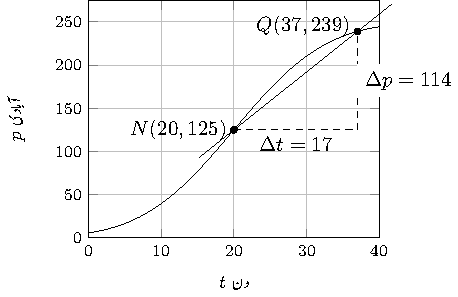
\includegraphics{normalDistributionFlies}
\caption{مکھی کی نمو آبادی}
\label{شکل_حد_مکھی_نمو_آبادی}
\end{minipage}\hfill
\begin{minipage}{0.45\textwidth}
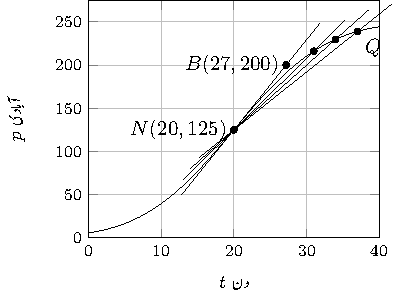
\includegraphics{normalDistributionFliesInstantaneous}
\caption{مکھی کی بیسویں دن نمو آبادی}
\label{شکل_حد_مکھی_نمو_آبادی_بیس}
\end{minipage}%
\end{figure}

حل:\quad
\عددی{20} ویں دن آبادی \عددی{125} تھی جبکہ \عددی{37} ویں دن آبادی \عددی{239} تھی۔ یوں \عددی{37-20=17} دنوں میں آبادی میں \عددی{239-125=114} تبدیل  رونما ہوئی۔یوں شرح تبدیلی درج ذیل ہو گی
\begin{align*}
\frac{\Delta p}{\Delta t}=\frac{114}{17}=6.7 (\text{\RL{مکھیاں فی دن}})
\end{align*}
جو شکل \حوالہ{شکل_حد_مکھی_نمو_آبادی} میں سیکنٹ \عددی{NQ} کی ڈھلوان ہے۔
\انتہا{مثال}
%========================

درج بالا مثال میں \عددی{20} ویں دن سے \عددی{37} ویں دن تک کی اوسط شرح تبدیلی حاصل کی گئی جو ہمیں \عددی{20} ویں دن کی تبدیلی کی شرح کے بارے میں کوئی معلومات فراہم نہیں کرتی ہے۔اس کے لئے ہمیں \عددی{20} ویں دن کے قریب حساب  کرنا ہو گا۔

\ابتدا{مثال}
مثال \حوالہ{مثال_حد_نمو_آبادی_مکھی} میں \عددی{20} ویں دن آبادی میں تبدیلی کی شرح کیا ہے؟\\
حل:\quad
ہمیں نقطہ \عددی{Q} کو نقطہ \عددی{N} کے قریب سے قریب تر کرتے ہوئے شرح حاصل کرنی ہو گی (شکل \حوالہ{شکل_حد_مکھی_نمو_آبادی_بیس})۔یوں درج ذیل حاصل ہوتا ہے۔
\begin{align*}
\begin{array}{ll}
Q&\frac{\Delta p}{\Delta t}\\
\hline
(37,239)&\frac{239-125}{37-20}=6.7\\
(35,230)&\frac{230-125}{35-20}=7\\
(32,216)&\frac{216-125}{32-20}=7.6\\
(27,200)&\frac{200-125}{27-20}=10.7
\end{array}
\end{align*}

جیسے جیسے \عددی{Q} کو بائیں منتقل کیا جائے، خط \عددی{NQ} نقطہ \عددی{N} کے گرد گھڑی کی الٹ رخ گھومتا ہے۔ہم دیکھتے ہیں کہ یہ خط آخر کار \عددی{NB} کو چھوتا ہے۔اس خط کو دیے گئے منحنی کا \اصطلاح{مماس}\فرہنگ{مماس}\حاشیہب{tangent}\فرہنگ{tangent} کہتے ہیں۔اس طرح ہم توقع کرتے ہیں کہ \عددی{20} ویں دن آبادی کی تبدیلی کی شرح \عددی{10.7} مکھیاں فی دن ہو گی۔
\انتہا{مثال}
%=======================

لمحہ \عددی{t=1} اور لمحہ \عددی{t=2} پر گرتے ہوئے پتھر کی رفتار یا \عددی{20} ویں دن شرح تبدیلی کو \اصطلاح{لمحاتی شرح تبدیلی}\فرہنگ{لمحاتی!شرح تبدیلی}\حاشیہب{instantaneous rates of change}\فرہنگ{instantaneous!rate of change} کہتے ہیں۔جیسا آپ نے دیکھا، ہم اوسط شرح تبدیلی کی تحدیدی قیمت سے لمحاتی شرح تبدیلی حاصل کرتے ہیں۔درج بالا مثال میں ہم نے خط مماس کو بطور خط سیکنٹ کی تحدیدی  صورت پیش کیا۔لمحاتی شرح اور مماس کا گہرا تعلق ہے جو دیگر موضوعات میں بھی پیش آتا ہے۔ اس تعلق کو مزید سمجھنے کی خاطر ہمیں  تحدیدی قیمتوں  کا تعین کرنا سیکھنا ہو گا جنہیں ہم \اصطلاح{حد}\فرہنگ{حد}\حاشیہب{limits}\فرہنگ{limits} کہتے ہیں۔ 

\جزوحصہء{تفاعل کی تحدیدی قیمتیں}
تحدیدی قیمت کی تعریف سے پہلی ایک اور مثال دیکھتے ہیں۔

\ابتدا{مثال}\شناخت{مثال_حد_عجیب_تفاعل_الف}
تفاعل \عددی{f(x)=\tfrac{x^2-1}{x-1}} نقطہ \عددی{x=1} کے قریب کیسا رویہ رکھتا ہے؟\\
حل:\quad
چونکہ صفر سے کسی بھی عدد کو تقسیم نہیں کیا جا سکتا ہے لہٰذا ماسوائے \عددی{x=1} کے، یہ کلیہ تمام حقیقی اعداد کے لئے \عددی{f} تعین کرتا ہے۔کسی بھی \عددی{x\ne 1} کے لئے ہم اس کلیہ کی سادہ صورت حاصل کر سکتے ہیں:
\begin{align*}
f(x)=\frac{x^2-1}{x-1}=\frac{(x-1)(x+1)}{x-1}=x+1\quad\quad (x\ne 1)
\end{align*} 
یوں خط \عددی{y=x+1} جس سے نقطہ \عددی{x=1} یعنی \عددی{(1,2)} خارج کیا گیا ہو اس تفاعل کو ظاہر کرتا ہے۔اس نقطہ کو شکل \حوالہ{شکل_مثال_حد_عجیب_تفاعل_الف} میں بطور سوراخ دکھایا گیا ہے۔اگرچہ نقطہ \عددی{f(1)} غیر معین ہے، ہم \عددی{ x} کی قیمت \عددی{1} کے قریب سے قریب لیتے ہوئے \عددی{f(x)} کی قیمت \عددی{2} کے جتنی قریب چاہیں کر سکتے ہیں۔
\begin{figure}
\centering
\begin{tikzpicture}
\draw[-latex](-1.5,0)--(3,0)node[right]{$x$};
\draw[-latex](0,-0.2)--(0,2.5)node[above]{$y$};
\draw[shorten <=-0.5cm,shorten >=-0.5cm](-1,0)--(1,2);
\foreach \x in {-1,1}{\draw(\x,0)node[below]{$\x$}--++(0,0.1);}
\foreach \y in {1,2}{\draw(0,\y)node[left]{$\y$}--++(0.1,0);}
\draw(1,2)node[ocirc]{};
\draw(0.5,1)node[right]{$y=f(x)=\tfrac{x^2-1}{x-1}$};
\end{tikzpicture}
\caption{شکل برائے مثال \حوالہ{مثال_حد_عجیب_تفاعل_الف}}
\label{شکل_مثال_حد_عجیب_تفاعل_الف}
\end{figure}
%
\begin{align*}
\begin{array}{ll}
\multicolumn{1}{c}{x (\ne 1)}&\multicolumn{1}{c}{f(x)=\tfrac{x^2-1}{x-1}=x+1,\,\, (x\ne 1)}\\
\hline
0.9&1.9\\
1.1&2.1\\
0.99&1.99\\
1.01&2.01\\
0.999&1.999\\
1.001&2.001\\
0.999999&1.999999\\
1.000001&2.000001
\end{array}
\end{align*}

ہم کہتے ہیں کہ \عددی{x} کی قیمت \عددی{1} تک پہنچنے سے \عددی{f(x)} کی قیمت \عددی{2} تک پہنچتی ہے یا \عددی{x} ایک تک پہنچنے سے \عددی{f(x)} تحدیدی قیمت \عددی{2} تک پہنچتی ہے یا حد \عددی{2} تک پہنچتی ہے، جس کو درج ذیل لکھا جاتا ہے۔
\begin{align*}
\lim_{x\to 1} f(x)=2 \quad \text{یا}\quad \lim_{x\to 1} \frac{x^2-1}{x-1}=2
\end{align*}
\عددی{x} کی قیمت \عددی{x_0} تک پہنچنے کو \عددی{x\to x_0} لکھا جاتا ہے۔
\انتہا{مثال}
%====================== 

\ابتدا{تعریف}\موٹا{حد کی غیر رسمی تعریف}\\
فرض کریں کہ \عددی{x_0} کی پڑوس میں ایک کھلے وقفہ پر تفاعل \عددی{f(x)} معین ہے۔یہ تفاعل نقطہ \عددی{x_0} پر غیر معین ہو سکتا ہے۔ اگر \عددی{x_0} کے کافی قریب \عددی{x} کی  تمام قیمتوں کے لئے \عددی{f(x)} کی قیمتیں \عددی{L} کے کافی قریب پائی جاتی ہوں تب ہم کہتے ہیں کہ \عددی{x} کی قیمت \عددی{x_0} تک پہنچنے سے \عددی{f} کی قیمت \اصطلاح{حد} \عددی{L} تک پہنچتی ہے۔ اس کو ہم درج ذیل لکھتے ہیں۔
\begin{align*}
\lim_{x\to x_0} f(x)=L
\end{align*}
\انتہا{تعریف}
%========================

اس تعریف کو غیر رسمی اس لئے کہا گیا ہے کہ "کافی قریب" کی طرز کے فقرے بہت ٹھیک نہیں ہیں۔خراد پر کام کرنے والے ماہر کے لئے کافی قریب سے مراد \عددی{\SI{10}{\micro\meter}} ہو سکتا ہے جبکہ ماہر فلکیات کے لئے اس کا مطلب چند ہزار نوری سال ہو سکتا ہے۔البتہ یہ تعریف اتنی درست ضرور ہے کہ ہم حد کو پہچان سکیں اور اس کی قیمت حاصل کر سکیں۔ہم حد کی بالکل ٹھیک تعریف جلد پیش کریں گے۔

\ابتدا{مثال}\شناخت{مثال_حد_عجیب_تفاعل_ب}
\عددی{x\to x_0} کی صورت میں \عددی{f} کی حد کی وجودیت \عددی{x_0} پر \عددی{f} کی تعریف کے تابع نہیں ہے۔ شکل \حوالہ{شکل_مثال_حد_عجیب_تفاعل_ب} میں  \عددی{f} کا \عددی{x\to 1} پر حد \عددی{2} ہے اگرچہ \عددی{x=1} پر \عددی{f} غیر معین ہے۔تفاعل \عددی{g} کا \عددی{x\to 1} پر حد \عددی{2} ہے اگرچہ \عددی{x=1} پر \عددی{g(1)=1} ہے۔یوں \عددی{\lim\limits_{x\to 1}g(x)\ne g(1)} ہو گا۔صرف تفاعل \عددی{h} کا \عددی{x\to 1} پر حد اور قیمت دونوں \عددی{2} کے برابر ہیں یعنی \عددی{\lim\limits_{x\to 1} h(x)=h(1)}۔
\begin{figure}
\centering
\begin{subfigure}{0.33\textwidth}
\centering
\begin{tikzpicture}[x=0.75cm]
\draw[-latex](-1.5,0)--(2,0)node[right]{$x$};
\draw[-latex](0,-0.2)--(0,2.5)node[above]{$y$};
\draw[shorten <=-0.5cm,shorten >=-0.5cm](-1,0)--(1,2);
\foreach \x in {-1,1}{\draw(\x,0)node[below]{$\x$}--++(0,0.1);}
\foreach \y in {1,2}{\draw(0,\y)node[left]{$\y$}--++(0.1,0);}
\draw(1,2)node[ocirc]{};
\draw(0,-1)node[font=\footnotesize]{$\begin{aligned}f(x)=\tfrac{x^2-1}{x-1}\end{aligned}$};
\end{tikzpicture}
\caption{}
\end{subfigure}%
\begin{subfigure}{0.33\textwidth}
\centering
\begin{tikzpicture}[x=0.75cm]
\draw[-latex](-1.5,0)--(2,0)node[right]{$x$};
\draw[-latex](0,-0.2)--(0,2.5)node[above]{$y$};
\draw[shorten <=-0.5cm,shorten >=-0.5cm](-1,0)--(1,2);
\foreach \x in {-1,1}{\draw(\x,0)node[below]{$\x$}--++(0,0.1);}
\foreach \y in {1,2}{\draw(0,\y)node[left]{$\y$}--++(0.1,0);}
\draw(1,2)node[ocirc]{};
\draw(1,1)node[circ]{};
\draw(0,-1)node[font=\footnotesize]{$\begin{aligned}g(x)=\begin{cases}\tfrac{x^2-1}{x-1},&x\ne 1\\ 1,&x=1\end{cases}\end{aligned}$};
\end{tikzpicture}
\caption{}
\end{subfigure}%
\begin{subfigure}{0.33\textwidth}
\centering
\begin{tikzpicture}[x=0.75cm]
\draw[-latex](-1.5,0)--(2,0)node[right]{$x$};
\draw[-latex](0,-0.2)--(0,2.5)node[above]{$y$};
\draw[shorten <=-0.5cm,shorten >=-0.5cm](-1,0)--(1,2);
\foreach \x in {-1,1}{\draw(\x,0)node[below]{$\x$}--++(0,0.1);}
\foreach \y in {1,2}{\draw(0,\y)node[left]{$\y$}--++(0.1,0);}
\draw(1,2)node[circ]{};
\draw(0,-1)node[font=\footnotesize]{$\begin{aligned}h(x)=x+1\end{aligned}$};
\end{tikzpicture}
\caption{}
\end{subfigure}%
\caption{$\lim\limits_{x\to 1} f(x)=\lim\limits_{x\to 1}g(x)=\lim\limits_{x\to 1} h(x)=2\quad $}
\label{شکل_مثال_حد_عجیب_تفاعل_ب}
\end{figure}
\انتہا{مثال}
%============================

بعض اوقات \عددی{\lim\limits_{x\to x_0}f(x)} کی قیمت \عددی{f(x_0)} سے حاصل کی جا سکتی ہے۔اس کی مثال تفاعل \عددی{f(x)} ہے جو کثیر رکنی اور تکونیاتی تفاعل کا الجبرائی مجموعہ  ہے اور جہاں \عددی{x_0} پر \عددی{f(x_0)} معین ہو۔

%===============================
\ابتدا{مثال}\شناخت{مثال_حد_عجیب_تفاعل_پ}
\begin{enumerate}[a.]
\item
$\lim\limits_{x\to 2} (4)=4$
\item
$\lim\limits_{x\to 13}(4)=4$
\item
$\lim\limits_{x\to 3} x=3$
\item
$\lim\limits_{x\to 2} (5x-3)=10-3=7$
\item
$\lim\limits_{x\to -2}\frac{3x+4}{x+5}=\frac{-6+4}{-2+5}=-\frac{2}{3}$
\end{enumerate}
\انتہا{مثال}
%================================
\ابتدا{مثال}\شناخت{مثال_حد_مماثل_تفاعل}
\begin{enumerate}[a.]
\item
اگر \عددی{f} مماثلی تفاعل \عددی{f(x)=x} ہو تب \عددی{x_0} کے کسی بھی قیمت کے لئے  درج ذیل ہو گا (شکل \حوالہ{شکل_مثال_حد_عجیب_تفاعل_پ}-ل)۔
\begin{align*}
\lim\limits_{x\to x_0} f(x)=\lim\limits_{x\to x_0} x=x_0
\end{align*}
\item
اگر \عددی{f} مستقل تفاعل \عددی{f(x)=k} ہو (جہاں \عددی{k} مستقل ہے) تب \عددی{x_0} کے کسی بھی قیمت کے لئے درج ذیل ہو گا (شکل \حوالہ{شکل_مثال_حد_عجیب_تفاعل_پ}-ب)۔
\begin{align*}
\lim\limits_{x\to x_0} f(x)=\lim\limits_{x\to x_0} k=k
\end{align*} 
\end{enumerate}
%
\begin{figure}
\centering
\begin{subfigure}{0.5\textwidth}
\centering
\begin{tikzpicture}
\draw[-latex](-0.25,0)--(3,0)node[right]{$x$};
\draw[-latex](0,-0.2)--(0,2)node[above]{$y$};
\draw[shorten <=-0.5cm](0,0)--(2,2)node[pos=1,left]{$y=x$};
\draw[dashed] (0,1)node[left]{$x_0$}--(1,1)--(1,0)node[below]{$x_0$};
\end{tikzpicture}
\caption{مماثل تفاعل}
\end{subfigure}%
\begin{subfigure}{0.5\textwidth}
\centering
\begin{tikzpicture}
\draw[-latex](-0.25,0)--(3,0)node[right]{$x$};
\draw[-latex](0,-0.2)--(0,2)node[above]{$y$};
\draw(-0.25,1)--(3,1)node[pos=0.9,above]{$y=k$};
\draw(0,1)node[circ]{}node[above left]{$k$};
\draw[dashed](1,0)node[below]{$x_0$}--(1,1)node[circ]{};
\draw(0,0)node[below left]{$M$};
\end{tikzpicture}
\caption{مستقل تفاعل}
\end{subfigure}%
\caption{اشکال برائے مثال \حوالہ{مثال_حد_عجیب_تفاعل_پ}}
\label{شکل_مثال_حد_عجیب_تفاعل_پ}
\end{figure}
\انتہا{مثال}
%==================================
\ابتدا{مثال}\شناخت{مثال_حد_عجیب_تفاعل_ت} \ترچھا{عین ممکن ہے کہ تفاعل کے دائرہ کار میں تفاعل کا حد نہ پایا جاتا ہو۔}\\ 
درج ذیل تفاعل کا \عددی{x\to 0} پر رویہ کیسا ہو گا؟
\begin{enumerate}[a.]
\item
$U(x)=\begin{cases}0,&x<0\\ 1,&x\ge 0  \end{cases}$
\item
$g(x)=\begin{cases} \tfrac{1}{x},&x\ne 0\\ 0,&x=0 \end{cases}$
\item
$f(x)=\begin{cases}0,&x\le 0\\ \sin \tfrac{1}{x},&x>0  \end{cases}$
\end{enumerate}
%

حل:\quad
\begin{enumerate}[a.]
\item
اکائی سیڑھی تفاعل \عددی{U(x)} کا \عددی{x\to 0} پر کوئی حد نہیں پایا جاتا ہے چونکہ اس نقطہ پر تفاعل کی چھلانگ پائی جاتی ہے۔\عددی{0} کے کافی قریب \عددی{x} کی منفی قیمتوں کے لئے \عددی{U} کی قیمت \عددی{0} ہے جبکہ \عددی{0} کے کافی  قریب  \عددی{x}  کی مثبت قیمتوں کے لئے \عددی{U} کی قیمت \عددی{1} ہے۔یوں \عددی{0} کے قریب پہنچنے سے \عددی{U} کی منفرد قیمت نہیں پائی جاتی ہے (شکل \حوالہ{شکل_مثال_حد_عجیب_تفاعل_ت}-ا)۔
\item
\عددی{x=0} کے کافی قریب تفاعل کی قیمت بے قابو بڑھتی ہے اور کسی ایک منفرد قیمت تک پہنچنے کی کوشش نہیں کرتی ہے (شکل \حوالہ{شکل_مثال_حد_عجیب_تفاعل_ت}-ب)۔
\item
\عددی{x=0} کے کافی قریب تفاعل بہت زیادہ ارتعاش کرتا ہے۔اس کی قیمت کسی مخصوص قیمت تک پہنچنے کی کوشش نہیں کرتی ہے (شکل \حوالہ{شکل_مثال_حد_عجیب_تفاعل_ت}-ج)۔ 
\end{enumerate}
%
\begin{figure}
\centering
\begin{subfigure}{0.33\textwidth}
\centering
\begin{tikzpicture}
\begin{axis}[clip=false,small,axis lines=middle,width=4cm,xtick={\empty},ytick={1},xlabel={$x$},ylabel={$y$},xlabel style={at={(current axis.right of origin)},anchor={west}},ylabel style={at={(current axis.above origin)},anchor=south},ymin=-0.5,ymax=2]
\addplot[domain=-2:0]{0};
\addplot[domain=0:2]{1};
\draw(axis cs:0,0)node[ocirc]{};
\draw(axis cs:0,1)node[circ]{};
\draw(axis cs:0,1)node[above right,font=\footnotesize]{$\begin{aligned}y=\begin{cases}0,&x<0\\ 1,&x\ge 1\end{cases}\end{aligned}$};
\end{axis}
\end{tikzpicture}
\caption{اکائی سیڑھی تفاعل $U(x)\,\,$}
\end{subfigure}%
\begin{subfigure}{0.33\textwidth}
\centering
\begin{tikzpicture}
\begin{axis}[clip=false,small,axis lines=middle,width=4cm,xtick={\empty},ytick={\empty},xlabel={$x$},ylabel={$y$},xlabel style={at={(current axis.right of origin)},anchor={west}},ylabel style={at={(current axis.above origin)},anchor=south}]
\addplot[domain=-4:-0.3]{1/x};
\addplot[domain=0.3:4]{1/x};
\draw(axis cs:0,0)node[circ]{}node[below right]{$0$};
\draw(axis cs:0.4,1)node[above right,font=\footnotesize]{$\begin{aligned}y=\begin{cases}\tfrac{1}{x},&x\ne 0\\ 0,&x=0\end{cases}\end{aligned}$};
\end{axis}
\end{tikzpicture}
\caption{$g(x)$}
\end{subfigure}%
\begin{subfigure}{0.33\textwidth}
\centering
\begin{tikzpicture}
\begin{axis}[clip=false,small,axis lines=middle,width=4cm,xtick={\empty},ytick={-1,1},xlabel={$x$},ylabel={$y$},xlabel style={at={(current axis.right of origin)},anchor={west}},ylabel style={at={(current axis.above origin)},anchor=south},ymin=-1.2,ymax=1.2]
\addplot[domain=-0.2:0]{0}node[circ]{};
\addplot[domain=0.052:0.08,samples=100]{sin(180/(pi*x)};
\addplot[domain=0.08:0.5,samples=100]{sin(180/(pi*x)};
\draw(axis cs:0,0)node[circ]{}node[below left]{$0$};
\draw(axis cs:0.2,-0.75)node[right,font=\footnotesize]{$\begin{aligned}y=\begin{cases}0 ,&x\le  0\\  \sin \tfrac{1}{x},&x>0\end{cases}\end{aligned}$};
\end{axis}
\end{tikzpicture}
\caption{$f(x)$}
\end{subfigure}%
\caption{اشکال برائے مثال \حوالہ{مثال_حد_عجیب_تفاعل_ت}}
\label{شکل_مثال_حد_عجیب_تفاعل_ت}
\end{figure}
\انتہا{مثال}
%=================================

\حصہء{سوالات \حوالہ{حصہ_حد_تبدیلی_کی_شرح_اور_حد}}

\موٹا{ترسیم سے حد}

\ابتدا{سوال}\شناخت{سوال_حد_ترسیم_سے_حد_الف}
شکل \حوالہ{شکل_سوال_حد_ترسیم_سے_حد_الف}-ا میں دی گئی ترسیم سے درج ذیل حد تلاش کریں یا حد نا ہونے کی وجہ بیان کریں۔
\begin{multicols}{3}
\begin{enumerate}[a.]
\item
$\lim\limits_{x\to 1} g(x)$
\item
$\lim\limits_{x\to 2} g(x)$
\item
$\lim\limits_{x\to 3}g(x)$
\end{enumerate}
\end{multicols}
%
\begin{figure}
\centering
\begin{subfigure}{0.5\textwidth}
\centering
\begin{tikzpicture}
\draw[-latex](-0.25,0)--(4,0)node[right]{$x$};
\draw[-latex](0,-0.2)--(0,1.5)node[above]{$y$};
\draw[dashed](0,1)node[left]{$1$}--(3,1)node[solid,circ]{};
\draw(-0.2,-0.2)--(1,1)node[ocirc]{};
\draw(1,0)node[circ]{}--(2,1)node[circ]{}node[above,yshift={2mm}]{$y=g(x)$}--(3,0)node[ocirc]{}--(3.9,0.9);
\foreach \x in {1,2,3}{\draw(\x,0)node[below]{$\x$}--++(0,0.1);}
\end{tikzpicture}
\caption{}
\end{subfigure}%
\begin{subfigure}{0.5\textwidth}
\centering
\begin{tikzpicture}
\draw[-latex](-3,0)--(2,0)node[right]{$t$};
\draw[-latex](0,-1.25)--(0,1.5)node[above]{$s$};
\draw(-3,-1)--(-2,0)node[ocirc]{}node[above,yshift={2mm}]{$s=f(t)$}--(-1,-1)node[circ]{}--(0,-1)node[ocirc]{}node[right]{$-1$};
\foreach \x in {-2,-1,1}{\draw(\x,0)node[below]{$\x$}--++(0,0.1);}
\draw(0,0)node[circ]{}node[below left]{$0$};
\draw(0,1)node[ocirc]{}node[left]{$1$}--(2,1);
\end{tikzpicture}
\caption{}
\end{subfigure}%
\caption{اشکال برائے سوال \حوالہ{سوال_حد_ترسیم_سے_حد_الف} اور سوال \حوالہ{سوال_حد_ترسیم_سے_حد_ب}}
\label{شکل_سوال_حد_ترسیم_سے_حد_الف}
\end{figure}
\انتہا{سوال}
%=====================
\ابتدا{سوال}\شناخت{سوال_حد_ترسیم_سے_حد_ب}
شکل \حوالہ{شکل_سوال_حد_ترسیم_سے_حد_الف}-ب میں دی گئی ترسیم سے درج ذیل حد تلاش کریں یا حد نا ہونے کی وجہ بیان کریں۔
\begin{multicols}{3}
\begin{enumerate}[a.]
\item
$\lim\limits_{t\to -2}f(t)$
\item
$\lim\limits_{t\to -1}f(t)$
\item
$\lim\limits_{t\to 0}f(t)$
\end{enumerate}
\end{multicols}
\انتہا{سوال}
%======================
\ابتدا{سوال}\شناخت{سوال_حد_ترسیم_سے_حد_پ}
تفاعل \عددی{y=f(x)}  (شکل \حوالہ{سوال_حد_ترسیم_سے_حد_پ}-ا) کے لئے درج ذیل فقروں میں سے کون سے درست ہیں؟
\begin{multicols}{3}
\begin{enumerate}[a.]
\item
$\lim\limits_{x\to 0}f(x)$ موجود ہے\\
\item
$\lim\limits_{x\to 0}f(x)=0$
\item
$\lim\limits_{x\to 0}f(x)=1$
\item
$\lim\limits_{x\to 1}f(x)=1$
\item
$\lim\limits_{x\to 1}f(x)=0$
\item
$\lim\limits_{x\to x_ 0}f(x)$
وقفہ \عددی{(-1,1)} میں ہر نقطہ \عددی{x_0} پر موجود ہے
\end{enumerate}
\end{multicols}
%
\begin{figure}
\centering
\begin{subfigure}{0.5\textwidth}
\centering
\begin{tikzpicture}
\draw[-latex](-1.2,0)--(3,0)node[right]{$x$};
\draw[-latex](0,-1.2)--(0,1.5)node[above]{$y$};
\draw(-1,-1)node[circ]{}--(0,0)node[ocirc]{}--(1,-1)node[ocirc]{} (1,0)node[circ]{}--(2,1)node[circ]{};
\draw(0,1)node[circ]{}node[left]{$1$}--++(0.1,0);
\foreach \x in {-1,1,2}{\draw(\x,0)node[below]{$\x$}--++(0,0.1);} 
\draw(0,-1)node[left]{$-1$}--++(0.1,0);
\draw(0.5,1.25)node[right]{$y=f(x)$};
\end{tikzpicture}
\caption{}
\end{subfigure}%
\begin{subfigure}{0.5\textwidth}
\centering
\begin{tikzpicture}[]
\draw[-latex](-1.2,0)--(3.5,0)node[right]{$x$};
\draw[-latex](0,-2.2)--(0,1.5)node[above]{$y$};
\foreach \x in {-1,1,2,3}{\draw(\x,0)node[below]{$\x$}--++(0,0.1);} 
\foreach \y in {-2,-1,1}{\draw(0,\y)node[left]{$\y$}--++(0.1,0);}
\draw(-1,-1)node[circ]{}--(0,0)node[circ]{};
\draw[domain=0:1] plot ({\x},{-2*\x*\x});
\draw([shift={(0:1)}]2,0) arc (0:180:1);
\draw(1,0)node[circ]{} (2,0)node[circ]{} (3,0)node[circ]{} (2,1)node[ocirc]{}node[above]{$y=f(x)$};
\end{tikzpicture}
\caption{}
\end{subfigure}%
\caption{اشکال برائے سوال \حوالہ{سوال_حد_ترسیم_سے_حد_پ} اور سوال \حوالہ{سوال_حد_ترسیم_سے_حد_ت}}
\label{شکل_سوال_حد_ترسیم_سے_حد_پ}
\end{figure}
\انتہا{سوال}
%============================
\ابتدا{سوال}\شناخت{سوال_حد_ترسیم_سے_حد_ت}
تفاعل \عددی{y=f(x)} (شکل \حوالہ{سوال_حد_ترسیم_سے_حد_پ}-ب)  کے لئے درج ذیل فقروں میں سے کون سے درست ہیں؟
\begin{multicols}{3}
\begin{enumerate}[a.]
\item
$\lim\limits_{x\to 2} f(x)$
موجود نہیں ہے
\item
$\lim\limits_{x\to 2}f(x)=2$
\item
$\lim\limits_{x\to 1}f(x)$
موجود نہیں ہے
\item
$\lim\limits_{x\to x_0}f(x)$
وقفہ \عددی{(-1,1)} میں ہر نقطہ \عددی{x_0} پر موجود ہے۔
\item
$\lim\limits_{x\to x_0}f(x)$
وقفہ \عددی{(1,3)} میں ہر نقطہ \عددی{x_0} پر موجود ہے۔
\end{enumerate}
\end{multicols}
\انتہا{سوال}
%======================

\موٹا{وجودیت اور حد}

سوال \حوالہ{سوال_حد_غیر_موجود_الف} اور سوال \حوالہ{سوال_حد_غیر_موجود_ب} میں حد کی غیر موجودگی کی وجہ بیان کریں۔

\ابتدا{سوال}\شناخت{سوال_حد_غیر_موجود_الف}
$\lim\limits_{x \to 0}\tfrac{x}{\abs{x}}$
\انتہا{سوال}
%======================
\ابتدا{سوال}\شناخت{سوال_حد_غیر_موجود_ب}
$\lim\limits_{x \to 1}\tfrac{1}{x-1}$
\انتہا{سوال}
%======================
\ابتدا{سوال}
فرض کریں کہ ماسوائے نقطہ \عددی{x=x_0} تفاعل \عددی{f(x)} تمام حقیقی \عددی{x} کے لئے معین ہے۔کیا \عددی{\lim\limits_{x\to x_0}f(x)} کی وجودیت کی وجودیت کے بارے میں کچھ کہنا ممکن ہے؟ اپنے جواب کی وجہ بیان کریں۔ 
\انتہا{سوال}
%======================
\ابتدا{سوال}
فرض کریں کہ  تفاعل \عددی{f(x)} وقفہ \عددی{[-1,1]} میں تمام  \عددی{x} کے لئے معین ہے۔کیا \عددی{\lim\limits_{x\to 0}f(x)} کے بارے میں کچھ کہنا ممکن ہے؟ اپنے جواب کی وجہ بیان کریں۔ 
\انتہا{سوال}
%======================
\ابتدا{سوال}
اگر \عددی{\lim\limits_{x\to 1}f(x)=5} ہو تب کیا \عددی{x=1} پر \عددی{f} کا معین ہونا لازم ہے؟اگر معین ہونا لازم ہو تب کیا \عددی{f(1)=5} ہونا لازم ہے؟ کیا \عددی{x=1} پر ہم \عددی{f} کی قیمت کے بارے میں کچھ کہہ سکتے ہیں؟ وضاحت کریں۔
\انتہا{سوال}
%======================
\ابتدا{سوال}
اگر \عددی{f(1)=5} ہو تب کیا \عددی{\lim\limits_{x\to 1}f(x)} لازماً موجود ہو گا؟ اگر ایسا ہو تب کیا \عددی{\lim\limits_{x\to 1}f(x)=5} لازماً ہو گا؟ کیا ہم  \عددی{\lim\limits_{x\to 1}f(x)} کے بارے میں کوئی نتیجہ اخذ کر سکتے ہیں؟ وضاحت کریں۔
\انتہا{سوال}
%======================

\موٹا{کیلکولیٹر اور کمپیوٹر کا استعمال}

\ابتدا{سوال}
\عددی{f(x)=\tfrac{x^2-9}{x+3}} لیں۔
\begin{enumerate}[a.]
\item
\عددی{f} کی قیمتوں کا جدول نقاط \عددی{x=-3.1,-3.01,-3.001,\cdots} پر وہاں تک تلاش کریں جہاں تک آپ کا کیلکولیٹر جواب حاصل کر سکتا ہو۔اس جدول سے \عددی{\lim\limits_{x\to -3}f(x)} کی اندازاً قیمت حاصل کریں۔اس کے برعکس نقاط \عددی{x=-2.9,-2.99,\cdots} پر \عددی{f} کی قیمتیں استعمال کرتے ہوئے نتیجہ کیا ہو گا؟
\item
تفاعل کو \عددی{x_0=-3} کے قریب ترسیم کریں۔ ترسیم پر \عددی{x\to -3} کے لئے \عددی{y} کی قیمت دیکھ کر  گزشتہ جزو کے نتائج کی تصدیق کریں۔ 
\item
\عددی{\lim\limits_{x\to -3}f(x)} کو الجبرائی طریقہ سے اخذ کریں۔
\end{enumerate}
\انتہا{سوال}
%=========================
\ابتدا{سوال}
\عددی{g(x)=\tfrac{x^2-2}{x-\sqrt{2}}} لیں۔
\begin{enumerate}[a.]
\item
\عددی{\sqrt{2}} کی تخمینی قیمتوں \عددی{x=1.4,1.41,1.414,\cdots} پر تفاعل کی قیمتوں کے جدول سے \عددی{\lim\limits_{x\to \sqrt{2}}g(x)}  کی اندازاً قیمت حاصل کریں۔
\item
نقطہ \عددی{x_0=\sqrt{2}} کے قریب تفاعل ترسیم کریں۔\عددی{x\to \sqrt{2}} کے لئے ترسیم سے \عددی{y} کی قیمت دیکھ کر گزشتہ جزو کی جواب کا تصدیق کریں۔
\item
\عددی{\lim\limits_{x\to\sqrt{2}}g(x)} کو الجبرائی طور پر حاصل کریں۔
\end{enumerate}
\انتہا{سوال}
%====================
\ابتدا{سوال}
\عددی{G(x)=\tfrac{x+6}{x^2+4x-12}} لیں۔
\begin{enumerate}[a.]
\item
نقاط \عددی{x=-5.9,-5.99,-5.999,\cdots} پر \عددی{G} کی قیمتوں کا جدول بنا کر \عددی{\lim\limits_{x\to -6}G(x)} کی اندازاً قیمت حاصل کریں۔ اس کے برعکس \عددی{x=-6.1,-6.01,-6.001,\cdots} پر \عددی{G} کی قیمتیں استعمال کرتے ہوئے کیا نتیجہ حاصل ہو گا؟
\item
\عددی{G} کو \عددی{x_0=6} کے قریبی نقطوں پر تقسیم کرتے ہوئے \عددی{x\to -6} کے لئے \عددی{G} کی قیمت دیکھ کر گزشتہ جزو کے نتائج کی تصدیق کریں۔
\item
\عددی{\lim\limits_{x\to -6}G(x)} کو الجبرائی طریقہ سے حاصل کریں۔
\end{enumerate}
\انتہا{سوال}
%======================
\ابتدا{سوال}
\عددی{h(x)=\tfrac{x^2-2x-3}{x^2-4x+3}} لیں۔
\begin{enumerate}[a.]
\item
نقاط \عددی{x=2.9, 2.99, 2.999,\cdots} پر \عددی{h} کی قیمتوں کے جدول سے \عددی{\lim\limits_{x\to 3}h(x)} کی اندازاً قیمت تلاش کریں۔اس کے برعکس \عددی{x=3.1,3.01,3.001,\cdots} پر \عددی{h} کی قیمتیں لیتے ہوئے نتیجہ کیا ہو گا؟
\item
\عددی{x_0=3} کے قریب \عددی{h} ترسیم کر کے \عددی{x\to 3} کے لئے \عددی{h(x)} کی قیمت دیکھ کر گزشتہ جزو کے نتائج کی تصدیق کریں۔
\item
\عددی{\lim\limits_{x\to 3}h(x)} کو الجبرائی طریقہ سے حاصل کریں۔
\end{enumerate}
\انتہا{سوال}
%=====================
\ابتدا{سوال}
\عددی{f(x)=\tfrac{x^2-1}{\abs{x}-1}} لیں۔
\begin{enumerate}[a.]
\item
\عددی{f} کی قیمتوں کا جدول \عددی{x} کی ان قیمتوں کے لئے بنائیں جو \عددی{x_0=-1} تک نیچے سے اور اوپر سے پہنچنے کی کوشش کرتی ہیں۔اس جدول سے \عددی{\lim\limits_{x\to-1}f(x)} کی اندازاً قیمت تلاش کریں۔  
\item
\عددی{x_0=-1} کے قریب \عددی{f} ترسیم کریں۔ترسیم سے \عددی{x\to -1} کے لئے \عددی{y} کی قیمتیں دیکھ کر گزشتہ جزو کے نتائج کی تصدیق کریں۔
\item
\عددی{\lim\limits_{x\to -1}f(x)} کو الجبرائی طریقہ سے حاصل کریں۔
\end{enumerate}
\انتہا{سوال}
%========================
\ابتدا{سوال}
\عددی{F(x)=\tfrac{x^2+3x+2}{2-\abs{x}}} لیں۔
\begin{enumerate}[a.]
\item
\عددی{F} کی قیمتوں کا جدول \عددی{x} کی ان قیمتوں کے لئے بنائیں جو \عددی{x_0=-2} تک نیچے سے اور اوپر سے پہنچنے کی کوشش کرتی ہیں۔اس جدول سے
 \عددی{\lim\limits_{x\to-2}F(x)} کی اندازاً قیمت تلاش کریں۔  
\item
\عددی{x_0=-2} کے قریب \عددی{F} ترسیم کریں۔ترسیم سے \عددی{x\to -2} کے لئے \عددی{y} کی قیمتیں دیکھ کر گزشتہ جزو کے نتائج کی تصدیق کریں۔
\item
\عددی{\lim\limits_{x\to -2}F(x)} کو الجبرائی طریقہ سے حاصل کریں۔
\end{enumerate}
\انتہا{سوال}
%========================
\ابتدا{سوال}
\عددی{g(\theta)=\tfrac{\sin\theta}{\theta}} لیں۔
\begin{enumerate}[a.]
\item
\عددی{g} کی قیمتوں کا جدول \عددی{\theta} کی ان قیمتوں کے لئے بنائیں جو \عددی{\theta_0=0} تک نیچے سے اور اوپر سے پہنچنے کی کوشش کرتی ہیں۔اس جدول سے
 \عددی{\lim\limits_{x\to 0}g(\theta)} کی اندازاً قیمت تلاش کریں۔  
\item
\عددی{\theta_0=0} کے قریب \عددی{g} ترسیم کریں۔ترسیم سے گزشتہ جزو کے نتائج کی تصدیق کریں۔
\end{enumerate}
\انتہا{سوال}
%========================
\ابتدا{سوال}
\عددی{G(t)=\tfrac{1-\cos t}{t^2}} لیں۔
\begin{enumerate}[a.]
\item
\عددی{G} کی قیمتوں کا جدول \عددی{t} کی ان قیمتوں کے لئے بنائیں جو \عددی{t_0=0} تک نیچے سے اور اوپر سے پہنچنے کی کوشش کرتی ہیں۔اس جدول سے
 \عددی{\lim\limits_{t\to 0}G(t)} کی اندازاً قیمت تلاش کریں۔  
\item
\عددی{t_0=0} کے قریب \عددی{G} ترسیم کریں۔ترسیم سے گزشتہ جزو کے نتائج کی تصدیق کریں۔
\end{enumerate}
\انتہا{سوال}
%===================
\ابتدا{سوال}
\عددی{f(x)=x^{\tfrac{1}{1-x}}} لیں۔
\begin{enumerate}[a.]
\item
\عددی{f} کی قیمتوں کا جدول \عددی{x} کی ان قیمتوں کے لئے بنائیں جو \عددی{x_0=1} تک نیچے سے اور اوپر سے پہنچنے کی کوشش کرتی ہیں۔کیا \عددی{x} کی قیمت \عددی{x\to 1} تک پہنچنے سے \عددی{f} کا تحدیدی نقطہ پایا جاتا ہے؟ اگر تحدیدی نقطہ پایا جاتا ہو، اس کا تلاش کریں۔اگر نہیں پایا جاتا ہو تب وجہ بیان کریں۔
\item
\عددی{x_0=1} کے قریب \عددی{f} ترسیم کریں۔ترسیم سے گزشتہ جزو کے نتائج کی تصدیق کریں۔
\end{enumerate}
\انتہا{سوال}
%=============================
\ابتدا{سوال}
\عددی{f(x)=\tfrac{3^x-1}{x}} لیں۔
\begin{enumerate}[a.]
\item
\عددی{f} کی قیمتوں کا جدول \عددی{x} کی ان قیمتوں کے لئے بنائیں جو \عددی{x_0=0} تک نیچے سے اور اوپر سے پہنچنے کی کوشش کرتی ہیں۔کیا
 \عددی{x} کی قیمت \عددی{x\to 0} تک پہنچنے سے \عددی{f} کا تحدیدی نقطہ پایا جاتا ہے؟ اگر تحدیدی نقطہ پایا جاتا ہو، اس کا تلاش کریں۔اگر نہیں پایا جاتا ہو تب وجہ بیان کریں۔
\item
\عددی{x_0=0} کے قریب \عددی{f} ترسیم کریں۔ترسیم سے گزشتہ جزو کے نتائج کی تصدیق کریں۔
\end{enumerate}
\انتہا{سوال}
%=============================
\موٹا{متغیر کی تحدیدی قیمت پر کرتے ہوئے حد کا تعین}

سوال \حوالہ{سوال_حد_پر_الف} تا سوال \حوالہ{سوال_حد_پر_ب} میں متغیر \عددی{x} کی تحدیدی قیمت کو تفاعل میں پر کرتے ہوئے تفاعل کی حد تلاش کریں۔

\ابتدا{سوال}\شناخت{سوال_حد_پر_الف}
$\lim\limits_{x\to 2} 2x$
\انتہا{سوال}
%========================
\ابتدا{سوال}
$\lim\limits_{x\to 0} 2x$
\انتہا{سوال}
%========================
\ابتدا{سوال}
$\lim\limits_{x\to \tfrac{1}{3}} (3x-1)$
\انتہا{سوال}
%========================
\ابتدا{سوال}
$\lim\limits_{x\to 1} -\tfrac{1}{3x-1}$
\انتہا{سوال}
%========================
\ابتدا{سوال}
$\lim\limits_{x\to -1} 3x(2x-1)$
\انتہا{سوال}
%========================
\ابتدا{سوال}
$\lim\limits_{x\to -1} \tfrac{3x^2}{2x-1}$
\انتہا{سوال}
%========================
\ابتدا{سوال}
$\lim\limits_{x\to \tfrac{\pi}{2}} x\sin x$
\انتہا{سوال}
%========================
\ابتدا{سوال}\شناخت{سوال_حد_پر_ب}
$\lim\limits_{x\to \pi} \tfrac{\cos x}{1-\pi}$
\انتہا{سوال}
%========================

\موٹا{اوسط شرح تبدیلی}

سوال \حوالہ{سوال_حد_اوسط_تبدیلی_شرح_الف} تا سوال \حوالہ{سوال_حد_اوسط_تبدیلی_شرح_ب} میں دیے وقفہ پر تفاعل کی اوسط شرح تبدیلی تلاش کریں۔

\ابتدا{سوال}\شناخت{سوال_حد_اوسط_تبدیلی_شرح_الف}
\عددی{f(x)=x^3+1}؛ (الف) \عددی{[2,3]}، (ب) \عددی{[-1,1]}
\انتہا{سوال}
%======================
\ابتدا{سوال}
\عددی{g(x)=x^2}؛ (الف) \عددی{[-1,1]}، (ب) \عددی{[-2,0]}
\انتہا{سوال}
%======================
\ابتدا{سوال}
\عددی{h(t)=\cos t}؛ (الف) \عددی{[\tfrac{\pi}{4},\tfrac{3\pi}{4}]}، (ب) \عددی{[\tfrac{\pi}{6},\tfrac{\pi}{2}]}
\انتہا{سوال}
%======================
\ابتدا{سوال}
\عددی{g(t)=2+\cos t}؛ (الف) \عددی{[0,\pi]}، (ب) \عددی{[-\pi,\pi]}
\انتہا{سوال}
%======================
\ابتدا{سوال}
\عددی{R(\theta)=\sqrt{4\theta+1}}؛  \عددی{[0,2]}
\انتہا{سوال}
%======================
\ابتدا{سوال}\شناخت{سوال_حد_اوسط_تبدیلی_شرح_ب}
\عددی{P(\theta)=\theta^3-4\theta^2+5\theta}؛  \عددی{[1,2]}
\انتہا{سوال}
%======================
\ابتدا{سوال}\شناخت{سوال_حد_چاند_الف}
چاند پر ساکن حالت سے گرنے والی چیز کا فاصلہ بالمقابل وقت ترسیم شکل \حوالہ{شکل_سوال_حد_چاند_الف} میں دکھایا گیا ہے۔ (الف) سیکنٹ \عددی{NQ_1}، \عددی{NQ_2}، \نقطے \عددی{NQ_6} کی اندازاً ڈھلوان تلاش کر کے جدول میں لکھیں۔ (ب) اس جدول سے \عددی{t=\SI{10}{\second}} پر رفتار کی اندازاً قیمت حاصل کریں۔
\begin{figure}
\centering
\begin{tikzpicture}
\begin{axis}[clip=false,small,axis lines=middle,grid=both,xlabel={ (سیکنڈ)$t$},ylabel={(میٹر)$y$}]
\addplot[domain=0:10]{1/2*1.6*x^2}node[circ]{}node[right]{$N$};
\draw(axis cs:5,20)node[circ]{}node[right]{$Q_1$};
\draw(axis cs:6,28.8)node[circ]{}node[right]{$Q_2$};
\draw(axis cs:7.07,40)node[circ]{}node[right]{$Q_3$};
\draw(axis cs:8,51.2)node[circ]{}node[right]{$Q_4$};
\draw(axis cs:8.66,60)node[circ]{}node[right]{$Q_5$};
\draw(axis cs:9.35,70)node[circ]{}node[right]{$Q_6$};
\end{axis}
\end{tikzpicture}
\caption{چاند پر ساکن حالت سے گرنے والی چیز کا فاصلہ بالمقابل وقت ترسیم}
\label{شکل_سوال_حد_چاند_الف}
\end{figure}
\انتہا{سوال}
%==================
\ابتدا{سوال}
ایک چھوٹی کمپنی کے پہلے چار سال کا منافع درج ذیل ہے۔(الف) منافع بالمقابل سال کو بطور نقطے ترسیم کرتے ہوئے انہیں ہموار ترین لکیر سے ملائیں۔ (ب)  \عددی{1992} اور \عددی{1994} کے بیچ منافع بڑھنے کی اوسط شرح تلاش کریں۔ (پ) ترسیم استعمال کرتے ہوئے \عددی{1992} کے دوران منافع بڑھنے کی شرح تلاش کریں۔
\begin{align*}
\begin{array}{rr}
\multicolumn{1}{c}{\text{سال}}&\multicolumn{1}{c}{\text{\RL{منافع (لاکھ)}}}\\
\hline
1990&6\\
1991&27\\
1992&62\\
1993&111\\
1994&174
\end{array}
\end{align*}
\انتہا{سوال}
%==========================
\ابتدا{سوال}
تفاعل \عددی{F(x)=\tfrac{x+2}{x-2}} کی قیمتیں نقطہ \عددی{x=2}، \عددی{\tfrac{11}{10}}، \عددی{\tfrac{101}{100}}، \عددی{\tfrac{1001}{1000}}، \عددی{\tfrac{10001}{10000}} اور \عددی{x=1} پر  حاصل کر کے جدول میں لکھیں۔(الف) جدول میں پائے جانے والے ہر \عددی{x\ne 1} کے لئے وقفہ \عددی{[1,x]} پر تفاعل کی اوسط شرح تبدیلی حاصل کریں۔ (ب) \عددی{x=1} پر \عددی{F(x)} کی شرح تبدیلی تلاش کریں۔اگر جدول بڑھانے کی ضرورت ہو تو جدول بڑھائیں۔ 
\انتہا{سوال}
%===========================
\ابتدا{سوال}
\عددی{x\ge 0} کے لئے \عددی{g(x)=\sqrt{x}} لیں۔
\begin{enumerate}[a.]
\item
وقفہ \عددی{[1,2]}، \عددی{[1,1.5]} اور \عددی{[1,1+h]} پر \عددی{x} کے  لحاظ سے \عددی{g(x)} کی اوسط شرح تبدیلی تلاش کریں۔
\item
صفر کے قریب \عددی{h} کی قیمتوں، مثلاً \عددی{h=0.1,0.01,0.001,0.0001,0.00001} کے لئے \عددی{x} کے لحاظ سے وقفہ \عددی{[1,1+h]} پر \عددی{g(x)} کی اوسط شرح تبدیلی تلاش کریں۔
\item
جدول سے \عددی{x=1} پر \عددی{g(x)} کی تبدیلی کی شرح کیا ہے؟
\item
\عددی{h\to 0} کے لئے \عددی{g(x)} کی تبدیلی کی شرح الجبرائی طریقہ سے حاصل کریں۔
\end{enumerate}
\انتہا{سوال}
%======================
\ابتدا{سوال}
\عددی{t\ne 0} کے لئے \عددی{f(t)=\tfrac{1}{t}} لیں۔
\begin{enumerate}[a.]
\item
(الف) وقفہ \عددی{t=2} تا \عددی{t=3} اور  (ب) وقفہ \عددی{t=2} تا \عددی{t=T} پر \عددی{t} کے لحاظ سے \عددی{g(t)} کی اوسط شرح تبدیلی تلاش کریں۔ 
\item
\عددی{2} تک پہنچنے والی \عددی{T} کی قیمتوں، مثلاً \عددی{T=2.1}، \عددی{T=2.01}، \عددی{T=2.001}، \عددی{T=2.0001}، \عددی{T=2.00001} اور \عددی{T=2.000001}، کے لئے وقفہ \عددی{[2,T]} پر \عددی{t} کے لحاظ سے \عددی{f(t)} کی اوسط شرح تبدیلی تلاش کر کر جدول میں لکھیں۔
\item
اس جدول سے \عددی{t=2} پر \عددی{t} کے لحاظ سے \عددی{f} کی شرح تبدیلی کیا ہے۔
\item
وقفہ \عددی{[2,T]} پر \عددی{t} کے لحاظ سے \عددی{f} کی شرح تبدیلی کی حد \عددی{T\to 2} کے لئے  تلاش کریں۔(\عددی{T=2} پر کرنے سے پہلے آپ کو کچھ الجبرا کرنا ہو گا۔)
\end{enumerate}
\انتہا{سوال}
%======================
سوال \حوالہ{سوال_حد_الجبرا_الف} تا سوال \حوالہ{سوال_حد_الجبرا_ب} کو کمپیوٹر کی مدد سے حل کریں۔(الف) نقطہ \عددی{x_0} کے قریب تفاعل ترسیم کریں۔ (ب) ترسیم کو دیکھ کر تفاعل کی حد کی اندازاً قیمت تلاش کریں۔ (پ) حد کو الجبرائی طور پر حاصل کریں۔

\ابتدا{سوال}\شناخت{سوال_حد_الجبرا_الف}
$\lim\limits_{x\to 2} \tfrac{x^4-16}{x-2}$
\انتہا{سوال}
%=========================
\ابتدا{سوال}
$\lim\limits_{x\to -1} \tfrac{x^3-x^2-5x-3}{(x+1)^2}$
\انتہا{سوال}
%=========================
\ابتدا{سوال}
$\lim\limits_{x\to 0} \tfrac{\sqrt[\leftroot{-2}3]{1+x}-1}{x}$
\انتہا{سوال}
%=========================
\ابتدا{سوال}
$\lim\limits_{x\to 3} \tfrac{x^2-9}{\sqrt{x^2+7}-4}$
\انتہا{سوال}
%=========================
\ابتدا{سوال}
$\lim\limits_{x\to 0} \tfrac{1-\cos x}{x\sin x}$
\انتہا{سوال}
%=========================
\ابتدا{سوال}\شناخت{سوال_حد_الجبرا_ب}
$\lim\limits_{x\to 0} \tfrac{2x^2}{3-3\cos x}$
\انتہا{سوال}
%=========================

\حصہ{حد تلاش کرنے کے قواعد}\شناخت{حصہ_حد_قواعد}
حد تلاش کرنے کے مسئلوں کو اس حصہ میں پیش کیا جائے گا۔پہلے تین مسئلے مثال \حوالہ{مثال_حد_مماثل_تفاعل} کے نتائج کو لے کر کثیر رکنی، ناطق تفاعل اور طاقتوں  کے حد تلاش کرنے میں ہمیں مدد دیتے ہیں۔چوتھا مسئلہ بعد میں استعمال ہونے والی حساب کے لئے ہمیں تیار کرتا ہے۔

\جزوحصہء{طاقتوں اور الجبرائی مجموعوں کے حد}

\ابتدا{مسئلہ}\شناخت{مسئلہ_حد_قواعد-الف}\موٹا{حد کے خواص}\\
اگر \عددی{\lim\limits_{x\to c}f(x)=L} اور \عددی{\lim\limits_{x\to c}g(x)=M} ہوں،جہاں \عددی{L} اور \عددی{M} حقیقی اعداد ہیں،  تب درج ذیل قواعد مطمئن ہوں گے۔
\begin{description}
\item{قاعدہ مجموعہ:}\quad 
$\lim\limits_{x\to c}[f(x)+g(x)]=L+M$
\item{قاعدہ فرق:}\quad
$\lim\limits_{x\to c}[f(x)-g(x)]=L-M$
\item{قاعدہ ضرب:}\quad
$\lim\limits_{x\to c}[f(x)\cdot g(x)]=L\cdot M$
\item{قاعدہ ضرب مستقل:}\quad
$\lim\limits_{x\to c} k f(x)=kL$
\quad
(\عددی{k} مستقل عدد ہے)
\item{قاعدہ حاصل تقسیم:}\quad
$\lim\limits_{x\to c}\tfrac{f(x)}{g(x)}=\tfrac{L}{M}$
\quad
$M\ne 0$
\item{قاعدہ طاقت:}\quad
اگر \عددی{m} اور \عددی{n} عدد صحیح ہوں تب
$\lim\limits_{x\to c}[f(x)]^{\tfrac{m}{n}}=L^{\tfrac{m}{n}}$
 ہو گا بشرطیکہ  \عددی{L^{\tfrac{m}{n}}} حقیقی عدد ہو۔
\end{description}
\انتہا{مسئلہ}
%============================

الفاظ میں درج بالا مسئلہ درج ذیل کہتا ہے۔
\begin{enumerate}
\item
دو تفاعل کے مجموعے کا حد ان تفاعل کے انفرادی حدوں کا مجموعہ ہو گا۔
\item
دو تفاعل کے فرق  کا حد ان تفاعل کے انفرادی حدوں کا فرق ہو گا۔
\item
دو تفاعل کے حاصل ضرب  کا حد ان تفاعل کے انفرادی حدوں کا حاصل ضرب  ہو گا۔
\item
ایک تفاعل ضرب مستقل کا حد اس تفاعل کے حد ضرب مستقل ہو گا۔
\item
دو تفاعل کے حاصل تقسیم کا حد ان تفاعل کے انفرادی حدوں کا حاصل تقسیم ہو گا بشرطیکہ نسب نما تفاعل کا حد غیر صفر ہو۔
\item
تفاعل کے ناطق طاقت کا حد اس تفاعل کے حد کا ناطق طاقت ہو گا بشرطیکہ حد کا ناطق طاقت  حقیقی عدد ہو۔ 
\end{enumerate}

قاعدہ مجموعہ کو حصہ میں جبکہ قاعدہ \عددی{2} تا \عددی{5}  کو ضمیمہ \حوالہ{ضمیمہ_ب} میں ثابت کیا گیا ہے۔قاعدہ \عددی{6} کا ثبوت اعلٰی درجے کی کتابوں میں پایا جائے گا۔

%===================
\ابتدا{مثال}\شناخت{مثال_حد_لمبا_تفاعل_الف}
\عددی{\lim\limits_{x\to c}\tfrac{x^3+4x^2-3}{x^2+5}} تلاش کریں۔\\
حل:\quad
مثال \حوالہ{مثال_حد_مماثل_تفاعل} کے نتائج \عددی{\lim\limits_{x\to c}x=c} اور \عددی{\lim\limits_{x\to c}k=k}  سے شروع کرتے ہوئے
 مسئلہ \حوالہ{مسئلہ_حد_قواعد-الف} کے مختلف شق استعمال کرتے ہوئے درج ذیل ملتا ہے۔

\begin{enumerate}[a.]
\item 
$\lim\limits_{x\to c} x^2=(\lim\limits_{x\to c} x)(\lim\limits_{x\to c}x)=c\cdot c=c^2$ \hfill 
حاصل ضرب یا طاقت
\item
$\lim\limits_{x\to c}(x^2+5)=\lim\limits_{x\to c}x^2+\lim\limits_{x\to c} 5=c^2+5$ \hfill
مجموعہ اور (ا)
\item
$\lim\limits_{x\to c} 4x^2=4\lim\limits_{x\to c}x^2=4c^2$\hfill
ضرب مستقل اور (ا) 
\item
$\lim\limits_{x\to c}(4x^2-3)=\lim\limits_{x\to c}4x^2-\lim\limits_{x\to c} 3=4c^2-3$ \hfill
فرق اور (ج)
\item
$\lim\limits_{x\to c}x^3=(\lim\limits_{x\to c}x^2)(\lim\limits_{x\to c} x)=c^2\cdot c=c^3$\hfill
حاصل ضرب اور (ا) یا طاقت
\item
$\lim\limits_{x\to c}(x^3+4x-3)=\lim\limits_{x\to c}x^3+\lim\limits_{x\to c}(4x^2-3)=c^3+4c^2-3$\hfill
  مجموعہ، (ج) اور (د)
\item
$\lim\limits_{x\to c}\tfrac{x^3+4x^2-3}{x^2+5}=\tfrac{\lim\limits_{x\to c}(x^3+4x^2-3)}{\lim\limits_{x\to c}(x^2+5)}=\tfrac{c^3+4c^2-3}{c^2+5}$\hfill
حاصل تقسیم، (ہ) اور (ب) 
\end{enumerate}
\انتہا{مثال}
%===================
\ابتدا{مثال}
\عددی{\lim\limits_{x\to -2}\sqrt{4x^2-3}} تلاش کریں۔\\
حل:\quad
\begin{align*}
\lim\limits_{x\to -2}\sqrt{4x^2-3}&=\sqrt{4(-2)^2-3}\quad\quad\quad  \text{\RL{مثال \حوالہ{مثال_حد_لمبا_تفاعل_الف}-د اور $n=\tfrac{1}{2}$ کے ساتھ قاعدہ طاقت}}\\
&=\sqrt{16-3}=\sqrt{13}
\end{align*}
\انتہا{مثال}
%=======================

مسئلہ \حوالہ{مسئلہ_حد_قواعد-الف} کے دو نتائج  کثیر رکنی اور ناطق تفاعل کا حد تلاش کرنے کو مزید آسان بناتے ہیں۔ \عددی{x\to c} کے لئے کثیر رکنی کا حد تلاش کرنے کی خاطر محض تفاعل کے کلیہ میں \عددی{x} کی جگہ \عددی{c} پر کریں۔ناطق تفاعل کا حد \عددی{x\to c} پر تلاش کرنے کی خاطر تفاعل کے کلیہ میں \عددی{x} کی جگہ \عددی{c} پر کریں بشرطیکہ نسب نما اس نقطہ پر غیر صفر ہو۔

\ابتدا{مسئلہ}\شناخت{مسئلہ_حد_قواعد_ب}\موٹا{کثیر رکنی کا حد متغیر میں مستقل پر کرنے سے حاصل ہو گا}\\
اگر \عددی{P(x)=a_nx^n+a_{n-1}x^{n-1}+\cdots+a_0} ہو تب درج ذیل ہو گا۔
\begin{align*}
\lim\limits_{x\to c} P(x)=P(c)=a_nc^n+a_{n-1}c^{n-1}+\cdots+a_0
\end{align*}
\انتہا{مسئلہ}
%==============================
\ابتدا{مسئلہ}\شناخت{مسئلہ_حد_قواعد_پ}\موٹا{غیر صفر نسب نما کی صورت میں ناطق تفاعل کا حد کلیہ میں متغیر کی جگہ مستقل پر کرنے سے حاصل ہو گا}\\
فرض کریں کہ \عددی{P(x)} اور \عددی{Q(x)} کثیر رکنی ہیں اور \عددی{Q(c)\ne 0} ہے تب درج ذیل ہو گا۔
\begin{align*}
\lim\limits_{x\to c} \frac{P(x)}{Q(x)}=\frac{P(c)}{Q(c)}
\end{align*}
\انتہا{مسئلہ}
%============================

\ابتدا{مثال}
\begin{align*}
\lim_{x\to -1}\frac{x^3+4x^2-3}{x^2+5}=\frac{(-1)^3+4(-1)^2-3}{(-1)^2+5}=\frac{0}{6}=0
\end{align*}
یہ ایک ہی قدم میں مثال \حوالہ{مثال_حد_لمبا_تفاعل_الف} کا حل ہے۔
\انتہا{مثال}
%========================

\جزوحصہء{صفر نسب نما کا الجبرائی طریقہ سے اسقاط}
مسئلہ \حوالہ{مسئلہ_حد_قواعد_پ} ناطق تفاعل پر صرف اس صورت قابل اطلاق ہے جب تحدیدی نقطہ  \عددی{c} پر تفاعل کا نسب نما غیر صفر ہو۔صفر نسب نما کی صورت میں بعض اوقات نسب نما اور شمار کنندہ کے مشترک اجزاء ضربی   کاٹتے ہوئے  \عددی{c} پر غیر صفر نسب نما حاصل کیا جا سکتا ہے۔اگر ایسا ممکن ہو تب مشترک اجزاء ضربی کاٹ کر \عددی{x} کی جگہ \عددی{c} پر کرنے سے حد حاصل کیا جا سکتا ہے۔درج ذیل مثال میں نسب نما اور شمار کنندہ دونوں \عددی{x=1} پر صفر ہیں۔یوں \عددی{(x-1)} ان کا مشترک جزو ضربی ہے جس کو کاٹا جا سکتا ہے۔

\ابتدا{مثال}\شناخت{مثال_حد_اجزاء_منسوخ_الف}\ترچھا{یکساں جزو کی منسوخی}\\
\عددی{\lim\limits_{x\to 1}\tfrac{x^2+x-2}{x^2-x}} تلاش کریں۔\\
حل:\quad
ہم \عددی{x=1} پر نہیں کر سکتے ہیں چونکہ ایسا کرنے سے صفر نسب نما حاصل ہو گا اور صفر سے کسی بھی عدد کو تقسیم نہیں کیا جا سکتا ہے۔البتہ ہم نسب نما اور شمار کنندہ کو اجزاء ضربی کی صورت میں لکھ کر ان کے مشترک اجزاء ضربی  کو آپس میں کاٹ سکتے ہیں۔
\begin{align*}
\frac{x^2+x-2}{x^2-x}&=\frac{(x+2)(x-1)}{x(x-1)}=\frac{x+2}{x}
\end{align*}
اب \عددی{x\ne 0} کی صورت میں  درج بالا کو حد تلاش کرنے کے لئے  استعمال کیا جا سکتا ہے۔یوں درج ذیل حاصل ہوتا ہے۔
\begin{align*}
\lim_{x \to 1} \frac{x^2+x-2}{x^2-x}=\lim_{x\to 1}\frac{x+2}{x}=\frac{1+2}{1}=3
\end{align*}
شکل \حوالہ{شکل_مثال_حد_اجزاء_منسوخ_الف} میں \عددی{y=\tfrac{x^2+x-2}{x^2-x}} اور \عددی{y=\tfrac{x+2}{x}} کے ترسیم دکھائے گئے ہیں۔یہ ترسیم صرف نقطہ \عددی{(1,3)} پر ایک دوسرے سے مختلف ہیں۔البتہ اس نقطہ پر دونوں تفاعل کا حد ایک جیسا ہے۔ 
%
\begin{figure}
\centering
\begin{subfigure}{0.5\textwidth}
\centering
\begin{tikzpicture}
\begin{axis}[small,axis lines=middle,xtick={-2,1},ytick={3},xlabel={$x$},ylabel={$y$},ylabel style={at={(current axis.above origin)},anchor=south}]
\addplot[domain=-4:-0.5]{(x+2)/x};
\addplot[domain=0.5:4]{(x+2)/x}node[pos=0.1,right]{$y=\frac{x^2+x-2}{x^2-x}$};
\draw(axis cs:1,3)node[ocirc]{}node[right]{$(1,3)$};
\end{axis}
\end{tikzpicture}
\caption{}
\end{subfigure}%
\begin{subfigure}{0.5\textwidth}
\centering
\begin{tikzpicture}
\begin{axis}[small,axis lines=middle,xtick={-2,1},ytick={3},xlabel={$x$},ylabel={$y$},ylabel style={at={(current axis.above origin)},anchor=south}]
\addplot[domain=-4:-0.5]{(x+2)/x};
\addplot[domain=0.5:4]{(x+2)/x}node[pos=0.1,right]{$y=\frac{x+2}{x}$};
\draw(axis cs:1,3)node[circ]{}node[right]{$(1,3)$};
\end{axis}
\end{tikzpicture}
\caption{}
\end{subfigure}%
\caption{ماسوائے نقطہ $(1,3)$ کے دونوں ترسیم یکساں ہیں}
\label{شکل_مثال_حد_اجزاء_منسوخ_الف}
\end{figure}
\انتہا{مثال}
%=====================
\ابتدا{مثال}\شناخت{مثال_حد_پیدا_مشترک_جزو_ضربی}\موٹا{ایک جیسے اجزاء پیدا کرتے ہوئے انہیں آپس میں منسوخ کرنا}\\
\عددی{\lim\limits_{h\to 0}\tfrac{\sqrt{2+h}-\sqrt{2}}{h}} تلاش کریں۔\\
حل:\quad
ہم \عددی{h=0} پر کرتے ہوئے حد تلاش نہیں کر سکتے ہیں اور نسب نم اور شمار کنندہ کے مشترک جزو ضربی نہیں پائے جاتے ہیں۔البتہ ہم نسب نما (اور شمار کنندہ) کو \ترچھا{جوڑی دار تعلق}\فرہنگ{جوڑی دار تعلق}\حاشیہب{conjugate expression}\فرہنگ{conjugate expression} \عددی{\sqrt{2+h}+\sqrt{2}} سے ضرب دیتے ہوئے  مشترک جزو ضربی پیدا کر سکتے ہیں۔نسب نما میں جذروں  کے بیچ علامت تبدیل کرتے ہوئے جوڑی دار تعلق حاصل ہوتا ہے۔
\begin{align*}
\frac{\sqrt{2+h}-\sqrt{2}}{h}&=\frac{\sqrt{2+h}-\sqrt{2}}{h}\cdot \frac{\sqrt{2+h}+\sqrt{2}}{\sqrt{2+h}+\sqrt{2}}\\
&=\frac{2+h-2}{h(\sqrt{2+h}+\sqrt{2})}\\
&=\frac{h}{h(\sqrt{2+h}+\sqrt{2})}&& \text{\RL{مشترک جزو ضربی پیدا کیا گیا ہے}}\\
&=\frac{1}{\sqrt{2+h}+\sqrt{2}}&& \text{\RL{جس کو ہم کاٹتے ہیں}}
\end{align*}
یوں درج ذیل ہو گا۔
\begin{align*}
\lim_{h\to 0}\frac{\sqrt{2+h}-\sqrt{2}}{h}&=\lim_{h\to 0}\frac{1}{\sqrt{2+h}+\sqrt{2}}\\
&=\frac{1}{\sqrt{2+0}+\sqrt{2}}\quad\quad \text{\RL{نسب نما اب $h=0$ پر صفر نہیں ہے}}\\
&=\frac{1}{2\sqrt{2}}
\end{align*}
%
\begin{figure}
\centering
\begin{tikzpicture}
\begin{axis}[clip=false,small,axis lines=middle,xtick={1,2,3.2},xticklabels={$1$,$2$,$2+h$},ytick={\empty},xlabel={$x$},ylabel={$y$}]
\addplot[domain=0:0.3]{sqrt(x)};
\addplot[domain=0.3:4]{sqrt(x)}node[below]{$y=\sqrt{x}$};
\draw[shorten >=-1cm, shorten <=-1cm](axis cs:2,1.4142)node[circ]{}node[left,yshift={2mm}]{$N(2,\sqrt{2})$}--(axis cs:3.2,1.7888)node[circ]{}node[left,yshift={2mm}]{$Q(2+h,\sqrt{2+h})$};
\draw[dashed](axis cs:2,0)--(axis cs:2,1.4142);
\draw[dashed](axis cs:3.2,0)--(axis cs:3.2,1.7888);
\end{axis}
\end{tikzpicture}
\caption{$Q\to N$ کرنے سے سیکنٹ $NQ$ کی ڈھلوان کا حد $\tfrac{1}{2\sqrt{2}}$ ہے}
\label{شکل_مثال_حد_پیدا_مشترک_جزو_ضربی}
\end{figure}

دھیان رہے کہ تفاعل \عددی{\tfrac{\sqrt{2+h}-\sqrt{2}}{h}} درحقیقت تفاعل \عددی{y=\sqrt{x}} پر نقطہ \عددی{N(2,\sqrt{2})} اور نقطہ \عددی{Q(2+h,\sqrt{2+h})} کے بیچ سیکنٹ کی ڈھلوان ہے اور \عددی{h\to 0} کرنے سے مراد \عددی{Q\to N} ہے۔نقطہ \عددی{Q} ترسیم پر \عددی{N} کے بائیں ہاتھ بھی ہو سکتا ہے۔ہم نے دیکھا کہ اس سیکنٹ کی تحدیدی قیمت \عددی{\tfrac{1}{2\sqrt{2}}} ہے۔ 
\انتہا{مثال}
%=====================

\جزوحصہء{مسئلہ بیچ}
درج ذیل مسئلہ ہمیں بعد میں آنے والے ابواب میں کئی قسم کے حد حاصل کرنے میں مدد دیگا۔اس کو مسئلہ بیچ اس لئے کہتے ہیں کہ اس کا تعلق ایسے تفاعل \عددی{f} سے ہے جس کی قیمتیں  تفاعل \عددی{g} اور تفاعل \عددی{h} کی قیمتوں کے بیچ  ہو اور جن کا نقطہ \عددی{c} پر ایک ہی حد \عددی{L} ہو۔ظاہر ہے کہ نقطہ \عددی{c} پر دونوں تفاعل کے بیچ  پھنسے ہوئے تفاعل کی  قیمت  \عددی{L} ہو گی (شکل \حوالہ{شکل_حد_بیچ})۔اس کا ثبوت ضمیمہ \حوالہ{ضمیمہ_ب} میں دیا گیا ہے۔  
\begin{figure}
\centering
\begin{minipage}{0.45\textwidth}
\centering
\begin{tikzpicture}
\draw[-latex](-0.25,0)--(4.5,0)node[right]{$x$};
\draw[-latex](0,-0.2)--(0,2)node[left]{$y$};
\draw(0.5,2) to [out=0,in=180](2,1) to [out=0,in=180] (2.5,1.3) to [out=0,in=-135](4,2)node[right]{$h$};
\draw(0.25,0.25) to [out=0,in=180](1,0.5) to [out=0,in=180](1.5,0.75) to [out=0,in=180](2,1) to [out=0,in=180](2.5,0.75) to [out=0,in=180] (4,0.25)node[right]{$g$};
\draw[](2,1) to [out=0,in=180](2.5,1.1) to [out=0,in=180]++(0.25,-0.25) to [out=0,in=180]++(0.25,0.4)to [out=0,in=180]++(0.25,-0.6)to [out=0,in=180](4,1.6)node[right]{$f$};
\draw(2,1) to [out=180,in=0] ++(-0.2,0) to [out=180,in=0] ++(-0.4,-0.2)to [out=180,in=0] ++(-0.4,0.2)to [out=180,in=0] ++(-0.4,0.2)to [out=180,in=0] ++(-0.4,-0.3);
\draw[dashed](2,1)--(0,1)node[ocirc,solid]{}node[left]{$L$};
\draw[dashed](2,1)node[ocirc,solid]{}--(2,0)node[ocirc,solid]{}node[below]{$c$};
\end{tikzpicture}
\caption{$f$ کی ترسیم $h$ اور $g$ کی ترسیم کے بیچ ہے۔}
\label{شکل_حد_بیچ}
\end{minipage}\hfill
\begin{minipage}{0.45\textwidth}
\centering
\begin{tikzpicture}
\draw[-latex](-1.5,0)--(3.5,0)node[right]{$x$};
\draw[-latex](0,-0.2)--(0,2.2)node[right]{$y$};
\draw[domain=-1.25:1.25] plot ({\x},{1+\x*\x/2})node[right]{$y=1+\tfrac{x^2}{2}$};
\draw[domain=-1.25:1.25] plot ({\x},{1-\x*\x/2})node[right,yshift={1mm}]{$y=1-\tfrac{x^2}{2}$};
\draw(0,1) to [out=0,in=180]++(0.6,0.03) to [out=0,in=180]++(0.6,0.35) to [out=0,in=145]++(0.2,-0.3)node[right]{$y=u(x)$};
\draw(0,1) to [out=180,in=0]++(-0.6,-0.03) to [out=180,in=0]++(-0.6,-0.35);
\foreach \x in {-1,1}{\draw(\x,0)node[below]{$\x$}--++(0,0.1);}
\draw(0,1)node[below left]{$1$};
\draw(0,2)node[left]{$2$}--++(0.1,0);
\end{tikzpicture}
\caption{شکل برائے مثال \حوالہ{مثال_حد_بیچ_الف}}
\label{شکل_مثال_حد_بیچ_الف}
\end{minipage}%
\end{figure}

%========================
\ابتدا{مسئلہ}\موٹا{مسئلہ بیچ}\\
فرض کریں کسی کھلے وقفہ جس میں \عددی{c} پایا جاتا ہو، میں (ممکن ہے کہ) ماسوائے \عددی{x=c} پر تمام \عددی{x} کے لئے
\begin{align*}
g(x)\le f(x)\le h(x)
\end{align*}
ہے۔مزید فرض کریں کہ 
\begin{align*}
\lim_{x\to c} g(x)=\lim_{x\to c}h(x)=L
\end{align*}
ہے۔تب \عددی{\lim\limits_{x\to c} f(x)=L} ہو گا۔
\انتہا{مسئلہ}
%=====================

\ابتدا{مثال}\شناخت{مثال_حد_بیچ_الف}
اگر تمام \عددی{x\ne 0} کے لئے \عددی{1-\tfrac{x^2}{4}\le u(x)\le 1+\tfrac{x^2}{2}} ہو تب \عددی{\lim\limits_{x\to0}u(x)} تلاش کریں۔\\
حل:\quad
چونکہ
\begin{align*}
\lim_{x\to 0} (1-\tfrac{x^2}{2})=1\quad \text{اور}\quad \lim_{x\to 0} (1+\tfrac{x^2}{2})=1
\end{align*}
ہیں لہٰذا مسئلہ بیچ کے تحت \عددی{\lim\limits_{x\to 0}u(x)=1} ہو گا (شکل \حوالہ{شکل_مثال_حد_بیچ_الف})۔
\انتہا{مثال}
%========================
\ابتدا{مثال}
دکھائیں کہ اگر \عددی{\lim\limits_{x\to c} \abs{f(x)}=0} ہو تب \عددی{\lim\limits_{x\to c} f(x)=0} ہو گا۔\\
حل:\quad
چونکہ \عددی{-\abs{f(x)}\le f(x)\le \abs{f(x)}} ہے، اور \عددی{-\abs{f(x)}} اور \عددی{\abs{f(x)}} کا حد \عددی{0} ہے لہٰذا مسئلہ بیچ کے تحت \عددی{f(x)} کا حد بھی \عددی{0} ہو گا۔ 
\انتہا{مثال}
%============================

\جزوحصہء{سوالات \حوالہ{حصہ_حد_قواعد}}
\موٹا{حد کا حساب}

سوال \حوالہ{سوال_حد_تلاش_الف} تا سوال \حوالہ{سوال_حد_تلاش_ب} میں حد تلاش کریں۔

\ابتدا{سوال}\شناخت{سوال_حد_تلاش_الف}
$\lim\limits_{x\to -7} (2x+5)$
\انتہا{سوال}
%===================
\ابتدا{سوال}
$\lim\limits_{x\to 12} (10-3x)$
\انتہا{سوال}
%===================
\ابتدا{سوال}
$\lim\limits_{x\to 2} (-x^2+5x-2)$
\انتہا{سوال}
%===================
\ابتدا{سوال}
$\lim\limits_{x\to -2} (x^3-2x^2+4x+8)$
\انتہا{سوال}
%===================
\ابتدا{سوال}
$\lim\limits_{t\to 6} 8(t-5)(t-7)$
\انتہا{سوال}
%===================
\ابتدا{سوال}
$\lim\limits_{s\to \tfrac{2}{3}} 3s(2s-1)$
\انتہا{سوال}
%===================
\ابتدا{سوال}
$\lim\limits_{x\to 2} \tfrac{x+3}{x+6}$
\انتہا{سوال}
%===================
\ابتدا{سوال}
$\lim\limits_{x\to 5} \tfrac{4}{x-7}$
\انتہا{سوال}
%===================
\ابتدا{سوال}
$\lim\limits_{y\to -5} \tfrac{y^2}{5-y}$
\انتہا{سوال}
%===================
\ابتدا{سوال}
$\lim\limits_{y\to 2} \tfrac{y+2}{y^2+5y+6}$
\انتہا{سوال}
%===================
\ابتدا{سوال}
$\lim\limits_{x\to -1} 3(2x-1)^2$
\انتہا{سوال}
%===================
\ابتدا{سوال}
$\lim\limits_{x\to -4} (x+3)^{1984}$
\انتہا{سوال}
%===================
\ابتدا{سوال}
$\lim\limits_{y\to -3} (5-y)^{\tfrac{4}{3}}$
\انتہا{سوال}
%===================
\ابتدا{سوال}
$\lim\limits_{z\to 0} (2z-8)^{\tfrac{1}{3}}$
\انتہا{سوال}
%===================
\ابتدا{سوال}
$\lim\limits_{x\to 0} \tfrac{3}{\sqrt{3h+1}+1}$
\انتہا{سوال}
%===================
\ابتدا{سوال}\شناخت{سوال_حد_تلاش_ب}
$\lim\limits_{h\to 0} \tfrac{5}{\sqrt{5h+4}+2}$
\انتہا{سوال}
%===================
سوال \حوالہ{سوال_حد_حساب_الف} تا سوال \حوالہ{سوال_حد_حساب_ب} میں حد تلاش کریں۔

\ابتدا{سوال}\شناخت{سوال_حد_حساب_الف}
$\lim\limits_{x\to 5} \tfrac{x-5}{x^2-25}$
\انتہا{سوال}
%===================
\ابتدا{سوال}
$\lim\limits_{x\to -3} \tfrac{x+3}{x^2+4x+3}$
\انتہا{سوال}
%===================
\ابتدا{سوال}
$\lim\limits_{x\to -5} \tfrac{x^2+3x-10}{x+5}$
\انتہا{سوال}
%===================
\ابتدا{سوال}
$\lim\limits_{x\to 2} \tfrac{x^2-7x+10}{x-2}$
\انتہا{سوال}
%===================
\ابتدا{سوال}
$\lim\limits_{t\to 1} \tfrac{t^2+t-2}{t^2-1}$
\انتہا{سوال}
%===================
\ابتدا{سوال}
$\lim\limits_{t\to -1} \tfrac{t^2+3t+2}{t^2-t-2}$
\انتہا{سوال}
%===================
\ابتدا{سوال}
$\lim\limits_{x\to -2} \tfrac{-2x-4}{x^3+2x^2}$
\انتہا{سوال}
%===================
\ابتدا{سوال}
$\lim\limits_{y\to 0} \tfrac{5y^3+8y^2}{3y^4-16y^2}$
\انتہا{سوال}
%===================
\ابتدا{سوال}
$\lim\limits_{u\to 1} \tfrac{u^4-1}{u^3-1}$
\انتہا{سوال}
%===================
\ابتدا{سوال}
$\lim\limits_{v\to 2} \tfrac{v^3-8}{v^4-16}$
\انتہا{سوال}
%===================
\ابتدا{سوال}
$\lim\limits_{x\to 9} \tfrac{\sqrt{x}-3}{x-9}$
\انتہا{سوال}
%===================
\ابتدا{سوال}
$\lim\limits_{x\to 4} \tfrac{4x-x^2}{2-\sqrt{x}}$
\انتہا{سوال}
%===================
\ابتدا{سوال}
$\lim\limits_{x\to 1} \tfrac{x-1}{\sqrt{x+3}-2}$
\انتہا{سوال}
%===================
\ابتدا{سوال}\شناخت{سوال_حد_حساب_ب}
$\lim\limits_{x\to -1} \tfrac{\sqrt{x^2+8}-3}{x+1}$
\انتہا{سوال}
%===================

\موٹا{قواعد حد کا استعمال}

\ابتدا{سوال}
فرض کریں کہ \عددی{\lim_{x\to 0}f(x)=1} اور \عددی{\lim_{x\to 0}g(x)=5} ہیں۔مسئلہ \حوالہ{مسئلہ_حد_قواعد-الف} کے کون سے اجزاء درج ذیل قدم الف، ب اور پ میں استعمال کیے گئے ہیں؟
\begin{align*}
\lim_{x\to 0}\frac{2f(x)-g(x)}{(f(x)+7)^{\tfrac{2}{3}}}&=\frac{\lim_{x\to 0}(2f(x)-g(x))}{\lim_{x\to 0}(f(x)+7)^{\tfrac{2}{3}}}&& \text{(الف)}\\
&=\frac{\lim_{x\to 0} 2f(x)-\lim_{x\to 0} g(x)}{(\lim_{x\to 0} (f(x)+7))^{\tfrac{2}{3}}}&&\text{(ب)}\\
&=\frac{2\lim_{x\to 0} f(x)-\lim_{x\to 0} g(x)}{(\lim_{x\to 0} f(x)+\lim_{x\to 0} 7)^{\tfrac{2}{3}}}&&\text{(پ)}\\
&=\frac{(2)(1)-(-5)}{(1+7)^{\tfrac{2}{3}}}=\frac{7}{4}
\end{align*}
\انتہا{سوال}
%======================
\ابتدا{سوال}
فرض کریں کہ \عددی{\lim_{x\to 1}h(x)=5}، \عددی{\lim_{x\to 1}p(x)=1} اور \عددی{\lim_{x\to 1}r(x)=2} ہیں۔مسئلہ \حوالہ{مسئلہ_حد_قواعد-الف} کے کون سے اجزاء درج ذیل قدم الف، ب اور پ میں استعمال کیے گئے ہیں؟
\begin{align*}
\lim_{x\to 1}\frac{\sqrt{5h(x)}}{p(x)(4-r(x))}&=\frac{\lim_{x\to 1} \sqrt{5h(x)}}{\lim_{x\to 1}(p(x)(4-r(x)))}&&\text{(الف)}\\
&=\frac{\sqrt{\lim_{x\to 1} 5h(x)}}{(\lim_{x\to 1} p(x))(\lim_{x\to 1}(4-r(x)))}&&\text{(ب)}\\
&=\frac{\sqrt{5\lim_{x\to 1}h(x)}}{(\lim_{x\to 1} p(x))(\lim_{x\to 1}4-\lim_{x\to 1} r(x))}&&\text{(پ)}\\
&=\frac{\sqrt{(5)(5)}}{(1)(4-2)}=\frac{5}{2}
\end{align*}
\انتہا{سوال}
%=======================
\ابتدا{سوال}
\عددی{\lim_{x\to c}f(x)=5} اور \عددی{\lim_{x\to c}g(x)=-2} لیتے ہوئے درج ذیل حاصل کریں۔
\begin{multicols}{2}
\begin{enumerate}[a.]
\item
$\lim_{x\to c} f(x)g(x)$
\item
$\lim_{x\to c} 2f(x)g(x)$
\item
$\lim_{x\to c} (f(x)+3g(x))$
\item
$\lim_{x\to c}\tfrac{f(x)}{f(x)-g(x)}$
\end{enumerate}
\end{multicols}
\انتہا{سوال}
%========================
\ابتدا{سوال}
\عددی{\lim_{x\to 4}f(x)=0} اور \عددی{\lim_{x\to 4}g(x)=-3} لیتے ہوئے درج ذیل حاصل کریں۔
\begin{multicols}{2}
\begin{enumerate}[a.]
\item
$\lim_{x\to 4} (g(x)+3)$
\item
$\lim_{x\to 4} xf(x)$
\item
$\lim_{x\to 4} (g(x))^2$
\item
$\lim_{x\to 4} \tfrac{g(x)}{f(x)-1}$
\end{enumerate}
\end{multicols}

\انتہا{سوال}
%=======================
\ابتدا{سوال}
\عددی{\lim_{x\to b}f(x)=7} اور \عددی{\lim_{x\to b}g(x)=-3} لیتے ہوئے درج ذیل حاصل کریں۔
\begin{multicols}{2}
\begin{enumerate}[a.]
\item
$\lim_{x\to b} (f(x)+g(x))$
\item
$\lim_{x\to b} f(x)\cdot g(x)$
\item
$\lim_{x\to b} 4g(x)$
\item
$\lim_{x\to b} \tfrac{f(x)}{g(x)}$
\end{enumerate}
\end{multicols}

\انتہا{سوال}
%=====================
\ابتدا{سوال}
\عددی{\lim_{x\to -2}p(x)=4}، \عددی{\lim_{x\to -2}r(x)=0} اور \عددی{\lim_{x\to -2}s(x)=-3} لیتے ہوئے درج ذیل حاصل کریں۔
\begin{multicols}{2}
\begin{enumerate}[a.]
\item
$\lim_{x\to -2} (p(x)+r(x)+s(x))$
\item
$\lim_{x\to -2} p(x)\cdot r(x)\cdot s(x)$
\item
$\lim_{x\to -2} \tfrac{-4p(x)+5r(x)}{s(x)}$
\end{enumerate}
\end{multicols}
\انتہا{سوال}
%=========================
\موٹا{اوسط تبدیلی شرح کے حد}

درج ذیل صورت کے حد کا سیکنٹ خطوط، مماس اور لمحاتی شرح کے ساتھ گہرا تعلق ہونے کی بنا یہ احصاء میں عموماً درپیش ہوتا ہے۔
\begin{align*}
\lim_{h\to 0}\frac{f(x+h)-f(x)}{h}
\end{align*}
سوال \حوالہ{سوال_حد_سیکنٹ_الف} تا سوال \حوالہ{سوال_حد_سیکنٹ_ب} میں اس حد کو دیے گئے \عددی{x} پر تفاعل \عددی{f(x)} کے لئے تلاش کریں۔

\ابتدا{سوال}\شناخت{سوال_حد_سیکنٹ_الف}
$f(x)=x^2,\quad x=1$
\انتہا{سوال}
%======================
\ابتدا{سوال}
$f(x)=x^2,\quad x=-2$
\انتہا{سوال}
%======================
\ابتدا{سوال}
$f(x)=3x-4,\quad x=2$
\انتہا{سوال}
%======================
\ابتدا{سوال}
$f(x)=\tfrac{1}{x},\quad x=-2$
\انتہا{سوال}
%======================
\ابتدا{سوال}
$f(x)=\sqrt{x},\quad x=7$
\انتہا{سوال}
%======================
\ابتدا{سوال}\شناخت{سوال_حد_سیکنٹ_ب}
$f(x)=\sqrt{3x+1},\quad x=0$
\انتہا{سوال}
%======================

\موٹا{مسئلہ بیچ کا استعمال}

\ابتدا{سوال}
اگر \عددی{-1\le x\le 1} کے لئے \عددی{\sqrt{5-2x}\le f(x)\le \sqrt{5-x^2}} ہو تب \عددی{\lim_{x\to 0}f(x)} تلاش کریں۔
\انتہا{سوال}
%========================
\ابتدا{سوال}
اگر تمام \عددی{x} کے لئے \عددی{2-x^2\le g(x)\le 2\cos x} ہو تب \عددی{\lim_{x\to 0}g(x)} تلاش کریں۔
\انتہا{سوال}
%===================
\ابتدا{سوال}
(الف) \quad
یہ دکھایا جا سکتا ہے کہ \عددی{0} کے قریب تمام \عددی{x} کے لئے درج ذیل عدم مساوات مطمئن ہوتا ہے۔
\begin{align*}
1-\frac{x^2}{6}<\frac{x\sin x}{2-2\cos x}<1
\end{align*}
اس سے درج ذیل کے بارے میں کیا معلومات فراہم ہوتی ہیں؟اپنے جواب کی وجہ پیش کریں۔
\begin{align*}
\lim_{x\to 0} \frac{x\sin x}{2-2\cos x}
\end{align*}
(ب)\quad
\عددی{-2\le x\le 2} کے لئے \عددی{y=1-\tfrac{x^2}{6}}، \عددی{y=\tfrac{x\sin x}{2-2\cos x}} اور \عددی{y=1} ترسیم کریں۔ \عددی{x\to 0} کرتے ہوئے ان  ترسیم کے رویہ پر تبصرہ کریں۔
\انتہا{سوال}
%=====================
\ابتدا{سوال}
(الف) \quad
درج ذیل عدم مساوات \عددی{0} کے قریب تمام \عددی{x} کے لئے مطمئن ہوتی ہے۔
\begin{align*}
\frac{1}{2}-\frac{x^2}{24}<\frac{1-\cos x}{x^2}<\frac{1}{2}
\end{align*} 
اس سے درج ذیل کے بارے میں کیا معلومات فراہم ہوتی ہیں۔اپنے جواب کی وجہ پیش کریں۔
\begin{align*}
\lim_{x\to 0}\frac{1-\cos x}{x^2}
\end{align*}
(ب)\quad
\عددی{-2\le x\le 2} کے لئے \عددی{y=\tfrac{1}{2}-\tfrac{x^2}{24}}، \عددی{y=\tfrac{1-\cos x}{x^2}} اور \عددی{y=\tfrac{1}{2}} ترسیم کریں۔ان ترسیم کا رویہ  \عددی{x\to 0} کرتے ہوئے کیسا ہے؟
\انتہا{سوال}
%==============

\موٹا{نظریہ اور مثالیں}

\ابتدا{سوال}
اگر \عددی{[-1,1]} میں \عددی{x} کے لئے \عددی{x^4\le f(x)\le x^2} اور \عددی{x<-1} اور \عددی{x>1} کے لئے \عددی{x^2\le f(x)\le x^4} ہو تب کن نقطوں \عددی{c} پر آپ کو \عددی{\lim_{x\to c}f(x)} خود بخود معلوم ہو گا؟ ان نقطوں پر حد کیا ہو گا؟
\انتہا{سوال}
%===============
\ابتدا{سوال}
فرض کریں کہ تمام \عددی{x\ne 2} کے لئے \عددی{g(x)\le f(x)\le h(x)} ہے اور مزید فرض کریں کہ \عددی{\lim_{x\to 2}g(x)=\lim_{x\to 2}h(x)=-5} ہے۔کیا \عددی{2} پر \عددی{f}، \عددی{g} اور \عددی{h} کی قیمتوں کے بارے میں کچھ کہا جا سکتا ہے؟ کیا \عددی{f(2)=0} ہو سکتا ہے؟ کیا \عددی{\lim_{x\to 2}f(2)=0} ہو سکتا ہے؟ اپنے جوابات کی وجہات پیش کریں۔
\انتہا{سوال}
%=================
\ابتدا{سوال}
اگر \عددی{\lim_{x\to 4}\tfrac{f(x)-5}{x-2}=1} ہو تب \عددی{\lim_{x\to 4}f(x)} کیا ہو گا؟
\انتہا{سوال}
%=========================
\ابتدا{سوال}
اگر \عددی{\lim_{x\to -2}\tfrac{f(x)}{x^2}=1} ہو تب (الف) \عددی{\lim_{x\to -2}f(x)} (ب) \عددی{\lim_{x\to -2}\tfrac{f(x)}{x}} تلاش کریں۔
\انتہا{سوال}
%====================
\ابتدا{سوال}
(الف) \quad
اگر \عددی{\lim_{x\to 2}\tfrac{f(x)-5}{x-2}=3} ہو تب \عددی{\lim_{x\to 2}f(x)} کیا ہو گا؟\\
(ب) \quad
اگر \عددی{\lim_{x\to 2} \tfrac{f(x)-5}{x-2}=4} ہو تب \عددی{\lim_{x\to 2}f(x)} کیا ہو گا؟
\انتہا{سوال}
%===================
\ابتدا{سوال}
اگر \عددی{\lim_{x\to 0}\tfrac{f(x)}{x^2}=1} ہو تب (الف) \عددی{\lim_{x\to 0} f(x)} اور (ب) \عددی{\lim_{x\to 0}\tfrac{f(x)}{x}} کیا ہوں گے؟
\انتہا{سوال}
%=======================

\موٹا{کمپیوٹر}

\ابتدا{سوال}
(الف)\quad
\عددی{\lim_{x\to 0}g(x)} حاصل کرنے کی خاطر \عددی{g(x)=x\sin\tfrac{1}{x}} ترسیم کریں۔ \عددی{x} کے قریب ترسیم کو بڑا کرتے ہوئے نتیجہ حاصل کریں۔\\
(ب)\quad
جزو (الف) کے جواب کو الجبرائی طریقہ سے حاصل کریں۔ 
\انتہا{سوال}
%======================
\ابتدا{سوال}
(الف)\quad
\عددی{h(x)=x^2\cos \tfrac{1}{x^3}} ترسیم کرتے ہوئے \عددی{x} کے قریب ترسیم کو بڑا کرتے ہوئے \عددی{\lim_{x\to 0}h(x)} تلاش کریں۔ \\
(ب)\quad
جزو (الف) کے نتیجہ کو الجبرا سے حاصل کریں۔
\انتہا{سوال}
%==========================

\حصہ{مطلوبہ قیمتیں اور حد کی تعریف}\شناخت{حصہ_حد_مطلوبہ_قیمتیں_اور_حد}
اس حصہ میں ہم حد کی با ضابطہ تعریف پیش کرتے ہیں۔یہ تعریف کسی بھی مثال کے لئے قابل استعمال ہو گی۔ اس سے پہلے ہم تفاعل کی خارجی قیمت کو مقررہ حدود کے اندر رکھنے کی خاطر اس کے داخلی قیمتوں پر غور کرتے ہیں۔

\جزوحصہء{خارجی قیمتوں کو مطلوبہ قیمتوں کے قریب رکھنا}
ہم بعض اوقات جاننا چاہتے ہیں کہ \عددی{x} کی کون سی قیمتیں  تفاعل \عددی{y=f(x)} کی قیمتوں کو کسی مخصوص مطلوبہ قیمت کے قریب رکھے گی۔کتنا قریب کا دارومدار درپیش مسئلہ پر ہو گا۔مثلاً پٹرول پمپ پر ہم آخری قطرہ حاصل کرنا چاہیں گے۔مرمت کے دوران  مستری انجن  کی  نلی کا قطر \عددی{\SI{50}{\micro\meter}} درستگی کے اندر رکھنا چاہے گا اور دوا ساز اجزاء کو قریبی ملی گرام تک ناپے گا۔

\ابتدا{مثال}\شناخت{مثال_حد_قابو_الف}\ترچھا{خطی تفاعل قابو کرنا}\\
تفاعل \عددی{y=2x-1} کے خارجی قیمت کو \عددی{y_0=7} کے \عددی{2} اکائی قریب رکھنے کی خاطر \عددی{x} کو \عددی{x_0=4} کے کتنا قریب رکھنا ضروری ہے؟\\
حل:\quad
ہم سے پوچھا گیا ہے کہ \عددی{x} کی کن قیمتوں کے لئے \عددی{\abs{y-7}<2} ہے۔جواب حاصل کرنے سے پہلے ہم  \عددی{\abs{y-7}} کو \عددی{x} کی صورت میں لکھتے ہیں۔
\begin{align*}
\abs{y-7}=\abs{(2x-1)-7}=\abs{2x-8}
\end{align*}
یوں ہم \عددی{x} کی وہ قیمتیں جاننا چاہتے ہیں جو عدم مساوات \عددی{\abs{2x-8}<2} کو مطمئن کرتے ہوں۔اس عدم مساوات کو حل کرتے ہیں۔
\begin{align*}
\abs{2x-8}&<2\\
-2<2x-8&<2\\
6<2x&<10\\
3<x&<5\\
-1<x-4&<1
\end{align*}
\عددی{x} کو \عددی{x_0=4} کے \عددی{1} اکائی کے اندر  رکھتے ہوئے \عددی{y} کی قیمت \عددی{y_0=7} کے \عددی{2} اکائیوں کے اندر رہے گی (شکل \حوالہ{شکل_مثال_حد_قابو_الف})۔
\begin{figure}
\centering
\begin{minipage}{0.45\textwidth}
\centering
\begin{tikzpicture}[x={0.25cm},y={0.25cm}]
\draw[-latex](-1,0)--(12,0)node[right]{$x$};
\draw[-latex](0,-2.5)--(0,12)node[above]{$y$};
\draw[dashed,name path=kA](0,9)node[left]{$9$}--++(12,0)node[pos=0.75,above]{\RL{بالائی سطح}}node[right]{$y=9$};
\draw[dashed,name path=kB](0,5)node[left]{$5$}--++(12,0)node[pos=0.75,above]{\RL{نچلی سطح}}node[right]{$y=5$};
\draw(0,7)node[circ]{}node[left]{$7$};
\draw[name path=kC](-0.5,-2)--(7,13)node[right]{$y=2x-1$};
\draw[dashed](3,0)node[below]{$3$}--(3,12);
\draw[dashed](5,0)node[below]{$5$}--(5,12);
\draw(4,0)node[circ]{}node[below]{$4$};
\draw [decorate,decoration={brace,amplitude=2pt},yshift=0pt](5,-2) -- (3,-2)node [black,midway,yshift=-9pt] {\footnotesize
\RL{یہ قابو کرتے ہوئے}};
\draw [decorate,decoration={brace,amplitude=2pt},xshift=-9pt,yshift=0pt](-1,5) -- (-1,9)node [black,midway,left,xshift=0pt] {\footnotesize
\RL{اس کو قابو کریں}};
\draw(4,7)node[circ]{};
\end{tikzpicture}
\caption{$x$ کی قیمت قابو کرتے ہوئے $y$ کی قیمت قابو کی جاتی ہے (مثال \حوالہ{مثال_حد_قابو_الف})}
\label{شکل_مثال_حد_قابو_الف}
\end{minipage}\hfill
\begin{minipage}{0.45\textwidth}
\centering
\begin{tikzpicture}
\begin{axis}[small,axis lines=middle,xlabel={$x$},ylabel={$y$},xtick={1.75,2.28},ytick={1.8,2.2}]
\addplot[domain=0.6667:0.8] {sqrt(3*x-2)};
\addplot[domain=0.8:3.2] {sqrt(3*x-2)}node[pos=0.9,left,xshift={-1mm}]{$y=\sqrt{3x-2}$};
\addplot[dashed] plot coordinates {(1.75,0) (1.75,1.8)};
\addplot[dashed]plot coordinates {(2.28,0) (2.28,2.2)};
\addplot[dashed] plot coordinates {(0,1.8) (4,1.8)};
\addplot[dashed]plot coordinates {(0,2.2) (4,2.2)};
\end{axis}
\end{tikzpicture}
\caption{$y$ کو $1.8$ اور $2.2$ کے اندر رکھنے کی خاطر $x$ کو $1.75$ اور $2.28$ کے اندر رکھنا ہو گا۔}
\label{شکل_مثال_حد_قابو_ب}
\end{minipage}
\end{figure}
\انتہا{مثال}
%==========================

\جزوحصہء{ٹیکنالوجی}
\ترچھا{مطلوبہ قیمتیں:}\quad
کمپیوٹر پر ترسیم کھینچ کر مطلوبہ قیمتوں پر تجربے کیے جا سکتے ہیں۔درکار تفاعل کی ترسیم پر بالائی اور نچلی مطلوبہ سطحوں کو افقی لکیروں سے ظاہر کریں۔ترسیم کو اتنا بڑا کریں کہ مطلوبہ وقفہ صاف نظر آئے۔یوں مطلوبہ وقفہ میں تفاعل کا رویہ دیکھا جا سکتا ہے۔

مثال کے طور پر \عددی{f(x)=\sqrt{3x-2}} کے ترسیم پر \عددی{y} محور کے مطلوبہ وقفہ \عددی{(1.8,2.2)} پر غور کریں۔یوں \عددی{y_1=f(x)}، \عددی{y_2=1.8} اور \عددی{y_3=2.2} ترسیم کریں (شکل \حوالہ{شکل_مثال_حد_قابو_ب})۔اسی طرح مطلوبہ وقفہ \عددی{(1.98,2.02)} اور \عددی{(1.9998,2.0002)} پر بھی تفاعل کا رویہ دیکھیں۔

\ابتدا{مثال}
\عددی{\SI{6}{\centi\meter}} اندرونی قطر کے ایک لڑر پیمائشی پیالے پر \عددی{\SI{1}{\milli\meter}} وقفہ پر افقی لکیریں کیوں کھینچی گئی ہوتی ہیں۔\\
پیالے میں مائع کا حجم \عددی{H=\pi r^2 h=36\pi h} ہو گا جہاں پیالے کا اندرونی رداس \عددی{r} اور مائع کی گہرائی \عددی{h} ہے۔ ایک لٹر \عددی{(\SI{1000}{\centi\meter\cubed})} پانی ناپنے کی خاطر \عددی{h} کتنا ہو گا؟ ناپ میں خلل \عددی{\SI{1}{\percent}} سے کم ہونا چاہیے۔\\
حل:\quad
ہم \عددی{h} کا ایسا وقفہ تلاش کرنا چاہتے ہیں کہ درج ذیل مطمئن ہوتا ہو۔
\begin{align*}
\abs{H-1000}=\abs{36\pi h-1000}\le 10
\end{align*}
یوں ہمیں درج ذیل عدم مساوات حل کرنی ہو گی۔
\begin{align*}
\abs{36\pi h-1000}&\le 10\\
-10\le 36\pi h-1000&\le 10\\
990\le 36\pi h&\le 1010\\
\tfrac{990}{36\pi}\le h &\le \tfrac{1010}{36\pi}\\
8.8\le h &\le 8.9
\end{align*}
یوں \عددی{\SI{1}{\percent}} درستگی کی خاطر درکار وقفہ گہرائی \عددی{8.9-8.8=\SI{0.1}{\centi\meter}} یعنی \عددی{\SI{1}{\milli\meter}} ہے۔پیالے پر ایک ملی میٹر فاصلے پر افقی لکیریں ہمیں ایک فی صد درستگی تک مائع ناپنے میں مدد دیتی ہیں جو کھانا تیار کرنے کے لئے کافی درستگی ہے۔
\انتہا{مثال}
%================

\جزوحصہء{حد کی با ضابطہ تعریف}
مطلوبہ قیمت مسئلے میں ہم جاننا چاہتے ہیں کہ متغیر \عددی{x} کو کسی مخصوص قیمت \عددی{x_0} کے کتنے قریب رکھتے ہوئے تفاعل \عددی{f(x)} کی قیمت کو مطلوبہ قیمت \عددی{y_0} کے قریب مخصوص وقفہ میں رکھنا ممکن ہو گا۔یہ دکھانے کی خاطر کہ \عددی{x\to x_0} کرنے سے \عددی{f(x)} کا حد \عددی{L} حاصل ہوتا ہے، ہمیں دکھانا ہو گا کہ ہم 
\عددی{x} کو \عددی{x_0} کے بہت قریب کرتے ہوئے  \عددی{f(x)} اور \عددی{L} میں فرق کو \ترچھا{کسی بھی معینہ خلل} سے کم کر سکتے ہیں۔

فرض کریں ہم  \عددی{f(x)} کی قیمت کو دیکھتے ہوئے \عددی{x} کو \عددی{x_0} کے قریب لاتے ہیں (تاہم  ہم \عددی{x} کی قیمت کو کبھی بھی \عددی{x_0} کے برابر نہیں کرتے ہیں)۔ہم چاہیں گے کہ ہم کہہ سکیں کہ \عددی{x_0} سے \عددی{x} کا فاصلہ \عددی{\delta} سے کم رکھنے سے \عددی{f(x)} اور \عددی{L} کی قیمت میں فرق \عددی{L} کی اکائی کے دسویں حصے  سے کم ہو گی (شکل \حوالہ{شکل_حد_تعریف_ایک_قدم})۔البتہ اتنا کافی نہیں ہے چونکہ \عددی{x} کو \عددی{x_0} کے مزید قریب کرنے سے کیا معلوم کہ وقفہ \عددی{L-\tfrac{1}{10}} تا \عددی{L+\tfrac{1}{10}} کے بیچ \عددی{f(x)} کی قیمت  \عددی{L} کے مزید قریب ہونے کی بجائے تھر تھراتی ہو۔
\begin{figure}
\centering
\begin{tikzpicture}
\draw[-latex](-0.25,0)--(4,0)node[right]{$x$};
\draw[-latex](0,-0.2)--(0,3.2)node[above]{$y$};
\draw(2,0)node[ocirc]{}node[below]{$x_0$};
\draw(1,0)node[]{$($}node[below]{$x_0-\delta$};
\draw(3,0)node[]{$)$}node[below]{$x_0+\delta$};
\draw(2.4,0)node[circ]{}node[above]{$x$};
\draw(0,1.5)node[left]{$L$}--++(0.1,0);
\draw(0,0.5)node[rotate=90]{$($}node[left,xshift={-1mm}]{$L-\tfrac{1}{10}$};
\draw(0,2.5)node[rotate=90]{$)$}node[left,xshift={-1mm}]{$L+\tfrac{1}{10}$};
\draw(0,2.1)node[circ]{}node[right]{$f(x)$};
\draw [decorate,decoration={brace,amplitude=10pt},yshift=10pt](1,0) -- (3,0)node [black,midway,yshift=15pt] {\footnotesize
\RL{یہاں تمام $x\ne x_0$ کے لئے}};
\draw [decorate,decoration={brace,amplitude=10pt},xshift=20pt](0,2.5) -- (0,0.5)node [black,midway,right,xshift=9pt] {\footnotesize
\RL{$f(x)$ یہاں رہے گا}};
\end{tikzpicture}
\caption{حد کی تعریف میں ایک قدم}
\label{شکل_حد_تعریف_ایک_قدم}
\end{figure}

ہمیں بتلایا جا سکتا ہے کہ  \عددی{\tfrac{L}{100}} یا \عددی{\tfrac{L}{1000}} یا \عددی{\tfrac{L}{100,000}} سے کم خلل کو برداشت کیا جا سکتا ہے۔ہر مرتبہ ہم \عددی {x_0} کے قریب  ایسا نیا وقفہ \عددی{\delta} تلاش کرتے ہیں جس کے اندر \عددی{x} رکھتے ہوئے قابل برداشت خلل کے اندر رہا جا سکتا ہے۔البتہ ہر مرتبہ اس امکان کو رد نہیں کیا جا سکتا ہے کہ \عددی{x_0} کے مزید قریب جانے سے  \عددی{f(x)} کی قیمت تھر تھراتے ہوئے \عددی{L} سے دور ہو جاتی ہو۔

شکل \حوالہ{شکل_حد_شکی_اور_عالم} میں اس مسئلے کی وضاحت کی گئی ہے جسے آپ ایک شکی انسان اور ایک عالم کے مابین بحث تصور کر سکتے ہیں۔شکی انسان قابل قبول خلل \عددی{\epsilon}  پیش کرتا ہے جس کے مقابلے میں عالم درکار \عددی{\delta} پیش کرتا ہے۔
\begin{figure}
\centering
\begin{subfigure}{0.5\textwidth}
\centering
\begin{tikzpicture}
\pgfmathsetmacro{\dY}{0.75}
\draw[-latex](0,0)--(4,0)node[right]{$x$};
\draw[-latex](0,0)--(0,2)node[above]{$y$};
\draw[name path=kC](0,0.10) to [out=45,in=-170] (2,1) to [out=10,in=-135](4,2);
\draw[dashed,name path=kA] (0,1+\dY)node[left]{$L+\tfrac{1}{10}$}--++(4,0);
\draw[dashed,name path=kB] (0,1-\dY)node[left]{$L-\tfrac{1}{10}$}--++(4,0);
\path[dashed,name path=kL](0,1)--++(4,0);
\draw[dashed,name intersections={of={kC and kL}}](0,1)--(intersection-1)node[circ]{}--($(0,0)!(intersection-1)!(4,0)$)node[below]{$x_0$};
\end{tikzpicture}
\caption{پہلا مقابلہ: $\abs{f(x)-L}< \epsilon=\tfrac{1}{10}$ کریں}
\end{subfigure}%
\begin{subfigure}{0.5\textwidth}
\centering
\begin{tikzpicture}
\pgfmathsetmacro{\dY}{0.75}
\draw[-latex](0,0)--(4,0)node[right]{$x$};
\draw[-latex](0,0)--(0,2)node[above]{$y$};
\draw[name path=kC](0,0.10) to [out=45,in=-170] (2,1) to [out=10,in=-135](4,2);
\draw[dashed,name path=kA] (0,1+\dY)node[left]{$L+\tfrac{1}{10}$}--++(4,0);
\draw[dashed,name path=kB] (0,1-\dY)node[left]{$L-\tfrac{1}{10}$}--++(4,0);
\path[dashed,name path=kL](0,1)--++(4,0);
\draw[dashed,name intersections={of={kC and kL}}](0,1)--(intersection-1)node[circ]{}--($(0,0)!(intersection-1)!(4,0)$)node[below]{$x_0$};
\draw[dashed,name intersections={of={kC and kA}}](0,1+\dY)--(intersection-1)--($(0,0)!(intersection-1)!(4,0)$)node[below]{$x_0-\delta_1$};
\draw[dashed,name intersections={of={kC and kB}}](0,1-\dY)--(intersection-1)--($(0,0)!(intersection-1)!(4,0)$)node[below]{$x_0+\delta_1$};
\end{tikzpicture}
\caption{پہلے جواب: $\abs{x-x_0}<\delta_1$ رکھیں}
\end{subfigure}
\begin{subfigure}{0.5\textwidth}
\centering
\begin{tikzpicture}
\pgfmathsetmacro{\dY}{0.35}
\draw[-latex](0,0)--(4,0)node[right]{$x$};
\draw[-latex](0,0)--(0,2)node[above]{$y$};
\draw[name path=kC](0,0.10) to [out=45,in=-170] (2,1) to [out=10,in=-135](4,2);
\draw[dashed,name path=kA] (0,1+\dY)node[left]{$L+\tfrac{1}{100}$}--++(4,0);
\draw[dashed,name path=kB] (0,1-\dY)node[left]{$L-\tfrac{1}{100}$}--++(4,0);
\path[dashed,name path=kL](0,1)--++(4,0);
\draw[dashed,name intersections={of={kC and kL}}](0,1)--(intersection-1)node[circ]{}--($(0,0)!(intersection-1)!(4,0)$)node[below]{$x_0$};
\end{tikzpicture}
\caption{دوسرا مقابلہ: $\abs{f(x)-L}< \epsilon=\tfrac{1}{100}$ کریں}
\end{subfigure}%
\begin{subfigure}{0.5\textwidth}
\centering
\begin{tikzpicture}
\pgfmathsetmacro{\dY}{0.35}
\draw[-latex](0,0)--(4,0)node[right]{$x$};
\draw[-latex](0,0)--(0,2)node[above]{$y$};
\draw[name path=kC](0,0.10) to [out=45,in=-170] (2,1) to [out=10,in=-135](4,2);
\draw[dashed,name path=kA] (0,1+\dY)node[left]{$L+\tfrac{1}{100}$}--++(4,0);
\draw[dashed,name path=kB] (0,1-\dY)node[left]{$L-\tfrac{1}{100}$}--++(4,0);
\path[dashed,name path=kL](0,1)--++(4,0);
\draw[dashed,name intersections={of={kC and kL}}](0,1)--(intersection-1)node[circ]{}--($(0,0)!(intersection-1)!(4,0)$)node[below]{$x_0$};
\draw[dashed,name intersections={of={kC and kA}}](0,1+\dY)--(intersection-1)--($(0,0)!(intersection-1)!(4,0)$)node[below]{$x_0-\delta_2$};
\draw[dashed,name intersections={of={kC and kB}}](0,1-\dY)--(intersection-1)--($(0,0)!(intersection-1)!(4,0)$)node[below]{$x_0+\delta_2$};
\end{tikzpicture}
\caption{دوسرا جواب: $\abs{x-x_0}<\delta_2$ رکھیں}
\end{subfigure}
\begin{subfigure}{0.5\textwidth}
\centering
\begin{tikzpicture}
\pgfmathsetmacro{\dY}{0.175}
\draw[-latex](0,0)--(4,0)node[right]{$x$};
\draw[-latex](0,0)--(0,2)node[above]{$y$};
\draw[name path=kC](0,0.10) to [out=45,in=-170] (2,1) to [out=10,in=-135](4,2);
\draw[dashed,name path=kA] (0,1+\dY)node[above left,solid]{$L+\tfrac{1}{1000}$}--++(4,0);
\draw[dashed,name path=kB] (0,1-\dY)node[below left,solid]{$L-\tfrac{1}{1000}$}--++(4,0);
\path[dashed,name path=kL](0,1)node[left]{$L$}--++(4,0);
\draw[dashed,name intersections={of={kC and kL}}](0,1)--(intersection-1)node[circ]{}--($(0,0)!(intersection-1)!(4,0)$)node[below]{$x_0$};
\end{tikzpicture}
\caption{تیسرا مقابلہ: $\abs{f(x)-L}< \epsilon=\tfrac{1}{1000}$ کریں}
\end{subfigure}%
\begin{subfigure}{0.5\textwidth}
\centering
\begin{tikzpicture}
\pgfmathsetmacro{\dY}{0.175}
\draw[-latex](0,0)--(4,0)node[right]{$x$};
\draw[-latex](0,0)--(0,2)node[above]{$y$};
\draw[name path=kC](0,0.10) to [out=45,in=-170] (2,1) to [out=10,in=-135](4,2);
\draw[dashed,name path=kA] (0,1+\dY)node[above left,solid]{$L+\tfrac{1}{1000}$}--++(4,0);
\draw[dashed,name path=kB] (0,1-\dY)node[below left,solid]{$L-\tfrac{1}{1000}$}--++(4,0);
\path[dashed,name path=kL](0,1)node[left]{$L$}--++(4,0);
\draw[dashed,name intersections={of={kC and kL}}](0,1)--(intersection-1)node[circ]{}--($(0,0)!(intersection-1)!(4,0)$)node[below]{$x_0$};
\draw[dashed,name intersections={of={kC and kA}}](0,1+\dY)--(intersection-1)--($(0,0)!(intersection-1)!(4,0)$)node[below,xshift={3mm}]{$x_0+\delta_3$};
\draw[dashed,name intersections={of={kC and kB}}](0,1-\dY)--(intersection-1)--($(0,0)!(intersection-1)!(4,0)$)node[below,xshift={-3mm}]{$x_0-\delta_3$};
\end{tikzpicture}
\caption{تیسرا جواب: $\abs{x-x_0}<\delta_3$ رکھیں}
\end{subfigure}%
\caption{شکی شخص اور عالم کا مقابلہ}
\label{شکل_حد_شکی_اور_عالم}
\end{figure}

اس نا ختم ہونے والی بحث کو ہم یوں ختم کر سکتے ہیں کہ ہم ثابت کریں کہ ہر \عددی{\sigma} کے لئے ایسا \عددی{\delta} تلاش کرنا ممکن ہے جو \عددی{f(x)} کو \عددی{L} کے  قریب قابل قبول فاصلہ \عددی{\epsilon} کے اندر رکھتا ہو (شکل \حوالہ{شکل_حد_تعریف})۔
\begin{figure}
\centering
\begin{tikzpicture}
\draw[-latex](-0.25,0)--(4,0)node[right]{$x$};
\draw[-latex](0,-0.2)--(0,3.2)node[above]{$y$};
\draw(2,0)node[ocirc]{}node[below]{$x_0$};
\draw(1,0)node[]{$($}node[below]{$x_0-\delta$};
\draw(3,0)node[]{$)$}node[below]{$x_0+\delta$};
\draw(2.4,0)node[circ]{}node[above]{$x$};
\draw(0,1.5)node[left]{$L$}--++(0.1,0);
\draw(0,0.5)node[rotate=90]{$($}node[left,xshift={-1mm}]{$L-\epsilon$};
\draw(0,2.5)node[rotate=90]{$)$}node[left,xshift={-1mm}]{$L+\epsilon$};
\draw(0,2.1)node[circ]{}node[right]{$f(x)$};
\draw [decorate,decoration={brace,amplitude=10pt},yshift=10pt](1,0) -- (3,0)node [black,midway,yshift=15pt] {\footnotesize
\RL{یہاں تمام $x\ne x_0$ کے لئے}};
\draw [decorate,decoration={brace,amplitude=10pt},xshift=20pt](0,2.5) -- (0,0.5)node [black,midway,right,xshift=9pt] {\footnotesize
\RL{$f(x)$ یہاں رہے گا}};
\end{tikzpicture}
\caption{حد کی تعریف میں $\delta$ اور $\epsilon$ کا تعلق۔}
\label{شکل_حد_تعریف}
\end{figure}

یوں آخر کار ہم ریاضی کی زبان میں یہ کہہ سکتے ہیں کہ \عددی{x} کو \عددی{x_0} کے جتنا زیادہ قریب کیا جائے، \عددی{f(x)} کی قیمت \عددی{L} کے اتنی قریب ہو گی۔

\ابتدا{تعریف}\موٹا{حد کی با ضابطہ تعریف}\\
فرض کریں کہ  \عددی{x_0} پر ایک کھلے وقفہ میں،  ممکنہ طور پر ماسوائے نقطہ \عددی{x_0} پر، \عددی{f(x)} معین ہے۔اگر ہر عدد \عددی{\epsilon>0} کے لئے ایسا مطابقتی عدد \عددی{\delta>0} پایا جاتا ہو کہ تمام \عددی{x} کے لئے درج ذیل مطمئن ہوتے ہوں  
\begin{align*}
0<\abs{x-x_0}<\delta,\quad \abs{f(x)-L}<\epsilon
\end{align*}
تب ہم کہتے ہیں کہ جیسے جیسے \عددی{x} کی قیمت \عددی{x_0} تک پہنچتی ہو ویسے ویسے \عددی{f(x)} کی قیمت حد \عددی{L} تک پہنچتی ہے جس کو الجبرائی طور پر درج ذیل لکھا جاتا ہے۔
\begin{align*}
\lim_{x\to x_0} f(x)=L
\end{align*} 
\انتہا{تعریف}
%=========================





%=========================================================
%\addcontentsline{toc}{chapter}{حوالہ}     %it is standard not to include References in toc. 
%\renewcommand*{\bibname}{حوالہ}      %this command has to be placed right here
%\begin{thebibliography}{99}\label{حوالہ_بیرونی_مواد}
%\begin{otherlanguage}{english}
%%\cite{حوالہ_کریزگ_الف_گیارہ}         this is how it is referenced in the text
%\bibitem{حوالہ_کریزگ_الف_سات}
 %Coddington, E. A. and N. Levinson, Theory of
%Ordinary Differential Equations. Malabar, FL: Krieger,
%1984.
%\bibitem{حوالہ_کریزگ_الف_گیارہ}
%Ince, E. L., Ordinary Differential Equations. New
%York: Dover, 1956.
%\bibitem{حوالہ_کریزگ_ب_اٹھارہ}
%Watson, G. N., A Treatise on the Theory of Bessel Functions. 2nd ed. Cambridge: University Press, 1944.
%\end{otherlanguage}
%\end{thebibliography}
%============================================================
\appendix
\باب{ضمیمہ دوم}\شناخت{ضمیمہ_ب}


%

%\include{./tex/emtEndOfBookTableDivergenceCurlGradientLaplacian}
%\include{./tex/toDoList}
%\include{./tex/emtQuestions}
\backmatter

\cleardoublepage
%\include{./tex/emtDataTables}        %appendices
%\include{./tex/emtLinearAlgebra}
%\include{./tex/emtCoordinatesRelations}
%================


%=================

\renewcommand*{\indexname}{فرہنگ}      %this command has to be placed right here just before printindex command
\cleardoublepage
\addcontentsline{toc}{chapter}{فرہنگ}
%\printindex


\end{urdufont}
\end{document}
